%%%%%%%%%%%%%%%%%%%%%%%%%%%%%%%%%%%%%%%%%
% Masters/Doctoral Thesis 
% LaTeX Template
% Version 2.2 (21/11/15)
%
% This template has been downloaded from:
% http://www.LaTeXTemplates.com
%
% Version 2.x major modifications by:
% Vel (vel@latextemplates.com)
%
% This template is based on a template by:
% Steve Gunn (http://users.ecs.soton.ac.uk/srg/softwaretools/document/templates/)
% Sunil Patel (http://www.sunilpatel.co.uk/thesis-template/)
%
% Template license:
% CC BY-NC-SA 3.0 (http://creativecommons.org/licenses/by-nc-sa/3.0/)
%
%%%%%%%%%%%%%%%%%%%%%%%%%%%%%%%%%%%%%%%%%

%----------------------------------------------------------------------------------------
%	PACKAGES AND OTHER DOCUMENT CONFIGURATIONS
%----------------------------------------------------------------------------------------

\documentclass[
12pt, % The default document font size, options: 10pt, 11pt, 12pt
%oneside, % Two side (alternating margins) for binding by default, uncomment to switch to one side
english, % ngerman for German
singlespacing %singlespacing, % Single line spacing, alternatives: onehalfspacing or doublespacing
%draft, % Uncomment to enable draft mode (no pictures, no links, overfull hboxes indicated)
%nolistspacing, % If the document is onehalfspacing or doublespacing, uncomment this to set spacing in lists to single
%liststotoc, % Uncomment to add the list of figures/tables/etc to the table of contents
%toctotoc, % Uncomment to add the main table of contents to the table of contents
%parskip, % Uncomment to add space between paragraphs
%nohyperref, % Uncomment to not load the hyperref package
headsepline, % Uncomment to get a line under the header
]{MastersDoctoralThesis} % The class file specifying the document structure

\usepackage[utf8]{inputenc} % Required for inputting international characters
\DeclareUnicodeCharacter{2113}{-}% support older LaTeX versions
\usepackage[T1]{fontenc} % Output font encoding for international characters

\usepackage{palatino} % Use the Palatino font by default
\usepackage{etoc}

\usepackage[backend=bibtex,style=alphabetic]{biblatex} % User the bibtex backend with the authoryear citation style (which resembles APA)

\usepackage{setspace}
\renewcommand{\baselinestretch}{1.1}
%\setstretch{baselinestretch}

\addbibresource{biblio.bib} % The filename of the bibliography

\usepackage[autostyle=true]{csquotes} % Required to generate language-dependent quotes in the bibliography

\usepackage[export]{adjustbox}

%\usepackage{cite}
\def\RR{\mathbb{R}}
\usepackage{amssymb}
\usepackage[cmex10]{amsmath}
%\usepackage{algorithm}
\usepackage{algorithmic}
\usepackage[titlenumbered,ruled,noend,english,onelanguage]{algorithm2e}

\newtheorem{lemma}{Lemma}
%\newcommand{\prox}{\mathrm{prox}}
%\DeclareMathOperator*{\argmin}{arg\,min}

%----------------------------------------------------------------------------------------
%	MARGIN SETTINGS
%----------------------------------------------------------------------------------------

\geometry{
	paper=a4paper, % Change to letterpaper for US letter
	inner=1.2cm, % Inner margin
	outer=2.5cm, % Outer margin
	bindingoffset=2cm, % Binding offset
	top=1.cm, % Top margin
	bottom=1.5cm, % Bottom margin
	%showframe,% show how the type block is set on the page
}
\usepackage{subcaption}
\usepackage{LpHypermodels}

%----------------------------------------------------------------------------------------
%	THESIS INFORMATION
%----------------------------------------------------------------------------------------

\thesistitle{Source localization for functional brain imaging with M/EEG} % Your thesis title, this is used in the title and abstract, print it elsewhere with \ttitle
\supervisor{Alexandre Gramfort \\ Roland Badeau} % Your supervisor's name, this is used in the title page, print it elsewhere with \supname
\examiner{Slim Essid} % Your examiner's name, this is not currently used anywhere in the template, print it elsewhere with \examname
\degree{Doctor of Philosophy} % Your degree name, this is used in the title page and abstract, print it elsewhere with \degreename
\author{Yousra Bekhti} % Your name, this is used in the title page and abstract, print it elsewhere with \authorname
\addresses{} % Your address, this is not currently used anywhere in the template, print it elsewhere with \addressname

\subject{Computer Science} % Your subject area, this is not currently used anywhere in the template, print it elsewhere with \subjectname
\keywords{} % Keywords for your thesis, this is not currently used anywhere in the template, print it elsewhere with \keywordnames
\university{%\href{http://www.telecom-paristech.fr/eng}
{T\'el\'ecom ParisTech}} % Your university's name and URL, this is used in the title page and abstract, print it elsewhere with \univname
\department{\href{http://www.tsi.telecom-paristech.fr/en/}{LTCI, TSI}} % Your department's name and URL, this is used in the title page and abstract, print it elsewhere with \deptname
\group{\href{http://www.tsi.telecom-paristech.fr/aao/en/}{AAO group}} % Your research group's name and URL, this is used in the title page, print it elsewhere with \groupname
\faculty{\href{http://faculty.university.com}{Faculty Name}} % Your faculty's name and URL, this is used in the title page and abstract, print it elsewhere with \facname

\hypersetup{pdftitle=\ttitle} % Set the PDF's title to your title
\hypersetup{pdfauthor=\authorname} % Set the PDF's author to your name
\hypersetup{pdfkeywords=\keywordnames} % Set the PDF's keywords to your keywords

\let\cleardoublepage\clearpage
\begin{document}

\frontmatter % Use roman page numbering style (i, ii, iii, iv...) for the pre-content pages

\pagestyle{plain} % Default to the plain heading style until the thesis style is called for the body content

%----------------------------------------------------------------------------------------
%	TITLE PAGE
%----------------------------------------------------------------------------------------

\begin{titlepage}
\begin{center}

\vspace*{0.05\textheight}
\textsc{\LARGE \univname}\\[1.cm] % University name
\textsc{\Large Mid-term Doctoral Thesis}\\[0.5cm] % Thesis type

\vspace{1.cm}

\HRule \\[0.4cm] % Horizontal line
{\huge \bfseries \ttitle}\\[0.4cm] % Thesis title
\HRule \\[1.5cm] % Horizontal line
 
\begin{minipage}{0.4\textwidth}
\begin{flushleft} \Large
\emph{Author:}\\
%\href{https://sites.google.com/site/yousrabekhti/}
{\authorname} % Author name - remove the \href bracket to remove the link
\end{flushleft}
\end{minipage}
\begin{minipage}{0.4\textwidth}
\begin{flushright} \Large
\emph{Supervisors:}\\%\href{http://alexandre.gramfort.net}
{\supname} % Supervisor name - remove the \href bracket to remove the link  
\end{flushright}
\end{minipage}\\[2cm]

\begin{minipage}{0.8\textwidth}
\begin{center} \large
Mid-term defense expected on May 18$^{th}$, 2016 with the \emph{Jury:}\\ \vspace{0.4cm}
Slim Essid: CNRS LTCI, T\'el\'ecom ParisTech\\ \vspace{0.2cm}
Matthieu Kowalski: Universit\'e Paris-Sud, L2S, Supélec\\ \vspace{2.cm}

\end{center}

\end{minipage}%\\[2cm]

\begin{figure}
%\centering
\begin{subfigure}[b]{5cm}          

\includegraphics[scale=0.5, left]{Figures/TelecomParisTech}
\end{subfigure}
%
\hspace{6.5cm}
%
\begin{subfigure}[b]{5cm}
%\centering

\includegraphics[scale=0.65]{CNRSfr}
\end{subfigure}
\end{figure}

\vfill
\end{center}
\end{titlepage}
\leavevmode\thispagestyle{empty}\newpage
% %----------------------------------------------------------------------------------------
%	QUOTATION PAGE
%----------------------------------------------------------------------------------------

\vspace*{0.2\textheight}

\noindent\enquote{\itshape Thanks to my solid academic training, today I can write hundreds of words on virtually any topic without possessing a shred of information, which is how I got a good job in journalism.}\bigbreak

\hfill Dave Barry
%----------------------------------------------------------------------------------------
%	ABSTRACT PAGE
%----------------------------------------------------------------------------------------
\leavevmode\thispagestyle{empty}\newpage

\begin{abstract}
\addchaptertocentry{\abstractname} % Add the abstract to the table of contents
\Ac{meg} and \ac{eeg} are non-invasive techniques for investigating human brain activity. They allow the measurement of ongoing brain activation on a millisecond-by-millisecond basis, which makes them very attractive to study the brain dynamics. Since the neuronal activity is measured at a sensor-level distributed over the head, the main question is how a brain region can be identified as the one producing the measured activity with reasonable accuracy? This is the so called bio-electromagnetic inverse problem which is ill-posed, meaning there is not a unique solution to the problem. The main goal of this thesis is the development of novel methods able to localize in space and time the origin of the observed head surface signals. \\

To do so, very challenging mathematical and computational problems need to be tackled. First of all, since the solution to the ill-posed inverse problem is not unique, constraints need to be set in order to identify an appropriate solution among the multiple possible candidates. The constraints are chosen depending on the assumptions or a priori knowledge based on the characteristics of the source distributions. Common priors are based on the Frobenius norm and lead to a family of methods generally referred to as minimum norm estimates (MNE). While these methods have some benefits like simple implementation and robustness to noise, they do not take into account the natural assumption that only a few brain regions are typically active during a specific cognitive task. Interestingly, several source reconstruction techniques have then been proposed, which are based on that assumption to promote focal or \textit{sparse} solutions. These techniques, which are partly used in clinical routine, are suitable, \textit{e.g.} for analyzing evoked responses or epileptic spike activity.\\

%Sparse source reconstruction has been investigated in both standard and time-frequency domains. Source localization in the standard domain implicitly assumes that the active sources are the same ones during the whole time interval of interest, \textit{i.e.} stationary sources. This also implies that if a source is detected as active at one time point, its activation will be non-zero over the entire time window. These solvers in the standard domain promote spatial sparsity only without modeling the dynamics and the non-stationarity of the brain signal. Therefore, they fail to recover realistic source estimates by mixing between time courses of different sources. %the true null activation during baseline (before the onset).
%In the other hand the source localization in the time-frequency domain addresses the problem of having non-stationary focal source activations. Using appropriate sparsity constraints, these solvers promote both spatial and temporal sparsity, which makes them recover better the non-stationary sources and the temporal smoothness. They have been investigated using a tight Gabor dictionary. However, the choice of an optimal dictionary for decomposing the brain signals remains unsolved.  Due to a mixture of signals, \textit{i.e.} short transient signals (right after the stimulus onset) and slower brain waves, the choice of a single dictionary explaining simultaneously both signals' types in a sparse way is difficult.\\

This thesis focuses first on the development of source solvers in the time-frequency domain to promote non-stationary focal source activation. %to overcome the problem of choosing the dictionary.
It introduces a novel method for improving the source estimation relying on a multi-scale dictionary, \textit{i.e.} multiple dictionaries with different scales concatenated to fit short transients and slow waves at the same time. We do not address the problem of learning the dictionary as doing so would make the cost function non-convex, which would deteriorate the speed of convergence, and also make the solver dependent on the initialization. \\%Our novel method was shown to outperform the basic solver in the time-frequency domain in terms of reduced leakage, temporal smoothness and in detection of both signal types.

A second project of this thesis is to investigate the hyperparameter estimation involved in the penalized regression way to formulate the problem. In the MEG/EEG community, the compromise between the data fit and the regularization controlled by $\lambda$ is often tuned by hand. This can be a tedious task very quickly, once you have to set it for several solvers and different datasets. This thesis introduces a new way to estimate this hyperparameter automatically when having a synthesis prior. This work has been based on a former paper of Marcelo Pereyra.\\

Since source estimates obtained with convex MEG/EEG sparse source imaging are biased in amplitude and often suboptimal in terms of sparsity, iterative reweighted mixed-norm solvers were applied which makes use of non-convex penalties in the time or the time-frequency domain. Also known as Majorization-minimization (MM), which is a standard iterative optimization technique which consists in minimizing a sequence of convex surrogate functionals. MM approaches have been particularly successful to tackle inverse problems and statistical machine learning problems where the regularization term is a sparsity-promoting concave function. However, due to non-convexity, the solution found by MM depends on its initialization. Uniform initialization is the most natural and often employed strategy as it boils down to penalizing all coefficients equally in the first MM iteration. Yet, this arbitrary choice can lead to unsatisfactory results in severely under-determined inverse problems such as MEG/EEG source imaging. The framework of hierarchical Bayesian modeling (HBM) is a seemingly unrelated approach to encode sparsity. This thesis shows that for certain hierarchical models, a simple alternating scheme to compute fully Bayesian MAP estimates leads to the exact same sequence of updates as a standard MM strategy (cf. the Adaptive \ac{lasso}). \\

Using simulation and various MEG/EEG datasets, this thesis provides empirical evidence that the novel methods presented here allow a promising estimation of MEG/EEG source reconstruction. A validation of these methods and a comparison with the widely used solvers is also presented using the phantom dataset (\textit{i.e.} a realistic dataset with groundtruth).\\

\textbf{keywords}--- Neuroimaging, magneto/electroencephalography (M/EEG), inverse problem, convex/non-convex optimization, sparse regression, multi-scale dictionaries, Gabor transform, hierarchical Bayesian models


\end{abstract}
\leavevmode\thispagestyle{empty}\newpage
%----------------------------------------------------------------------------------------
%	ACKNOWLEDGEMENTS
%----------------------------------------------------------------------------------------

\begin{acknowledgements}
\addchaptertocentry{\acknowledgementname} % Add the acknowledgements to the table of contents

First and formost I want to express my sincere gratitude to my advisor, Alexandre Gramfort, PhD., for his valuable guidance, support, encouragements and availability during these 3 short years of my PhD. I also want to thank him for introducing me to such a great multidisciplinary world, it was a great pleasure working on sophisticated problem modeling applied to Neuroscience. Your joy and enthusiasm was motivational for me and thanks for all the funding you made available for going all around the world for sake of Science. I would also like to thank, Roland Badeau, PhD., for accepting me in his team, and for our valuable discussions trying to reduce the gap between signal processing communities in both Music and Neuroscience research.\\

Thanks to Daniel Strohmeier, PhD., for his valuable advices at the beginning and all along my PhD, and for his time answering all my questions. I also want to thank Felix Lucka and Joseph Salmon for the awesome project we have got together, it was a great pleasure working with you, where I learned a lot. Also thanks to Virginie van Wassenhove for having me as an external collaborator at Neurospin - CEA Saclay where we have done great work together. I am also grateful for everyone in the MNE development team for their feedbacks of my work and reviewing my code to be integrated.
\\

Thanks to all my colleagues at the "Image, Data, Signal" department at Télécom ParisTech for the awesome working environment. Thanks to my closest colleagues, Mainak Jas, Tom Dupré la Tour, Stanislas Chambon for our several discussions about my work and your valuable feedbacks. It has been a pleasure working and sharing the B412 with you. I also want to thank Thierry Guillemot for introducing the Monday cake, everyone had the chance to discover their cooking skills, and we loved having your lemon pie.\\

Thanks to my music team "Les Airs Andalous" for their support all along my PhD, handling between work and concerts. You are my second family in Paris far away from my home. Thank you.\\

Finally, my family: \\
My parents: Fatima Zohra Benmansour and Mokhtar Bekhti. They gave me my name, they gave me my life, and the motivation of pursuing a PhD. I am so grateful for all your support and for always being here when needed. My siblings: SidiMohamed, Nihel, Abderrahmane and Amina, thank you for the awesome moments living together far from Tlemcen. I miss you already. I am not forgetting the latest Bekhti: Hadi, my nephew who is still 2 years old but still giving me all the inspiration when looking at him. To finish, a big thanks to my beloved, Sami Meziane for his priceless encouragement and patience, you are the best.\\

My final thoughts go to Raghav RV, it was nice having you with us, may you rest in peace.

{\raggedleft Yousra Bekhti\\}
{\raggedleft Paris, November 2017\\}
\end{acknowledgements}
%----------------------------------------------------------------------------------------
%	DEDICATION
%----------------------------------------------------------------------------------------

\dedicatory{\small{To my parents.}}
\leavevmode\thispagestyle{empty}\newpage
%----------------------------------------------------------------------------------------
%	LIST OF CONTENTS/FIGURES/TABLES PAGES
%----------------------------------------------------------------------------------------

\tableofcontents % Prints the main table of contents
\etocsettocstyle{}{} % from now on only local tocs
% \listoffigures % Prints the list of figures

% \listoftables % Prints the list of tables
%%----------------------------------------------------------------------------------------
%	SYMBOLS
%----------------------------------------------------------------------------------------

\begin{symbols}{lll} % Include a list of Symbols (a three column table)

$a$ & distance & \si{\meter} \\
$P$ & power & \si{\watt} (\si{\joule\per\second}) \\
%Symbol & Name & Unit \\

\addlinespace % Gap to separate the Roman symbols from the Greek

$\omega$ & angular frequency & \si{\radian} \\

\end{symbols}
%----------------------------------------------------------------------------------------
%	Introduction PAGE
%----------------------------------------------------------------------------------------

\addchaptertocentry{Introduction}

\newpage

{\huge\textbf{Introduction}\par}
\HRule \\[0.4cm] % Horizontal line
\section*{Context of the thesis}
%\textbf{Keywords:} Brain Imaging, Neuroscience Neurons, cells, Clinical work, cognitive science\\
%=> Non-invasive techniques/scanning - fMRI, M/EEG (functional)\\
%=> Why it is important to get back (inverse problem) to the brain? Ex: Epilepsy for clinical case or more how the brain works for a cognitive task.

Understanding the full complexity of the brain has been a challenging research project for decades, yet there are many mysteries that remain unsolved.
Being able to model how the brain represents, analyzes, processes, and transforms information of millions of different tasks in a record time is primordial for both a cognitive and clinical studies. These tasks can go from language, perception, memory, attention, emotion to reasoning and creativity. Studying the behavior of the brain at each task and extracting information to define its involved network will result in a better understanding of its functions. This has been widely used in other fields such as Artificial Intelligence where scientists and engineers try to implement aspects they learned from the human brain in computers. Unlike the cognitive science questions, in the clinical diagnostic, understanding how a pathology is affecting the brain, helps to find a cure or a way to improve patients' life. For example, being able to detect autism in early age of childhood, helps the parents to have a specific education and a better future.\\

To make this brain scanning possible, several cutting-edge technologies are used  depending on the question one is asking. These techniques differ from their degree of invasiveness, and their spatial and temporal resolution as it can be seen in the Figure~\ref{fig:brain_imaging_techniques}.
For the different tasks I mentioned above, one very important aspect is time. The brain is able to process most of the tasks in a fraction of a second, for example to recognize an emotion, to perceive a familiar face, etc. In this thesis, to study this high temporal resolution of the brain, I was interested in two direct brain imaging techniques.\\

\begin{figure}
	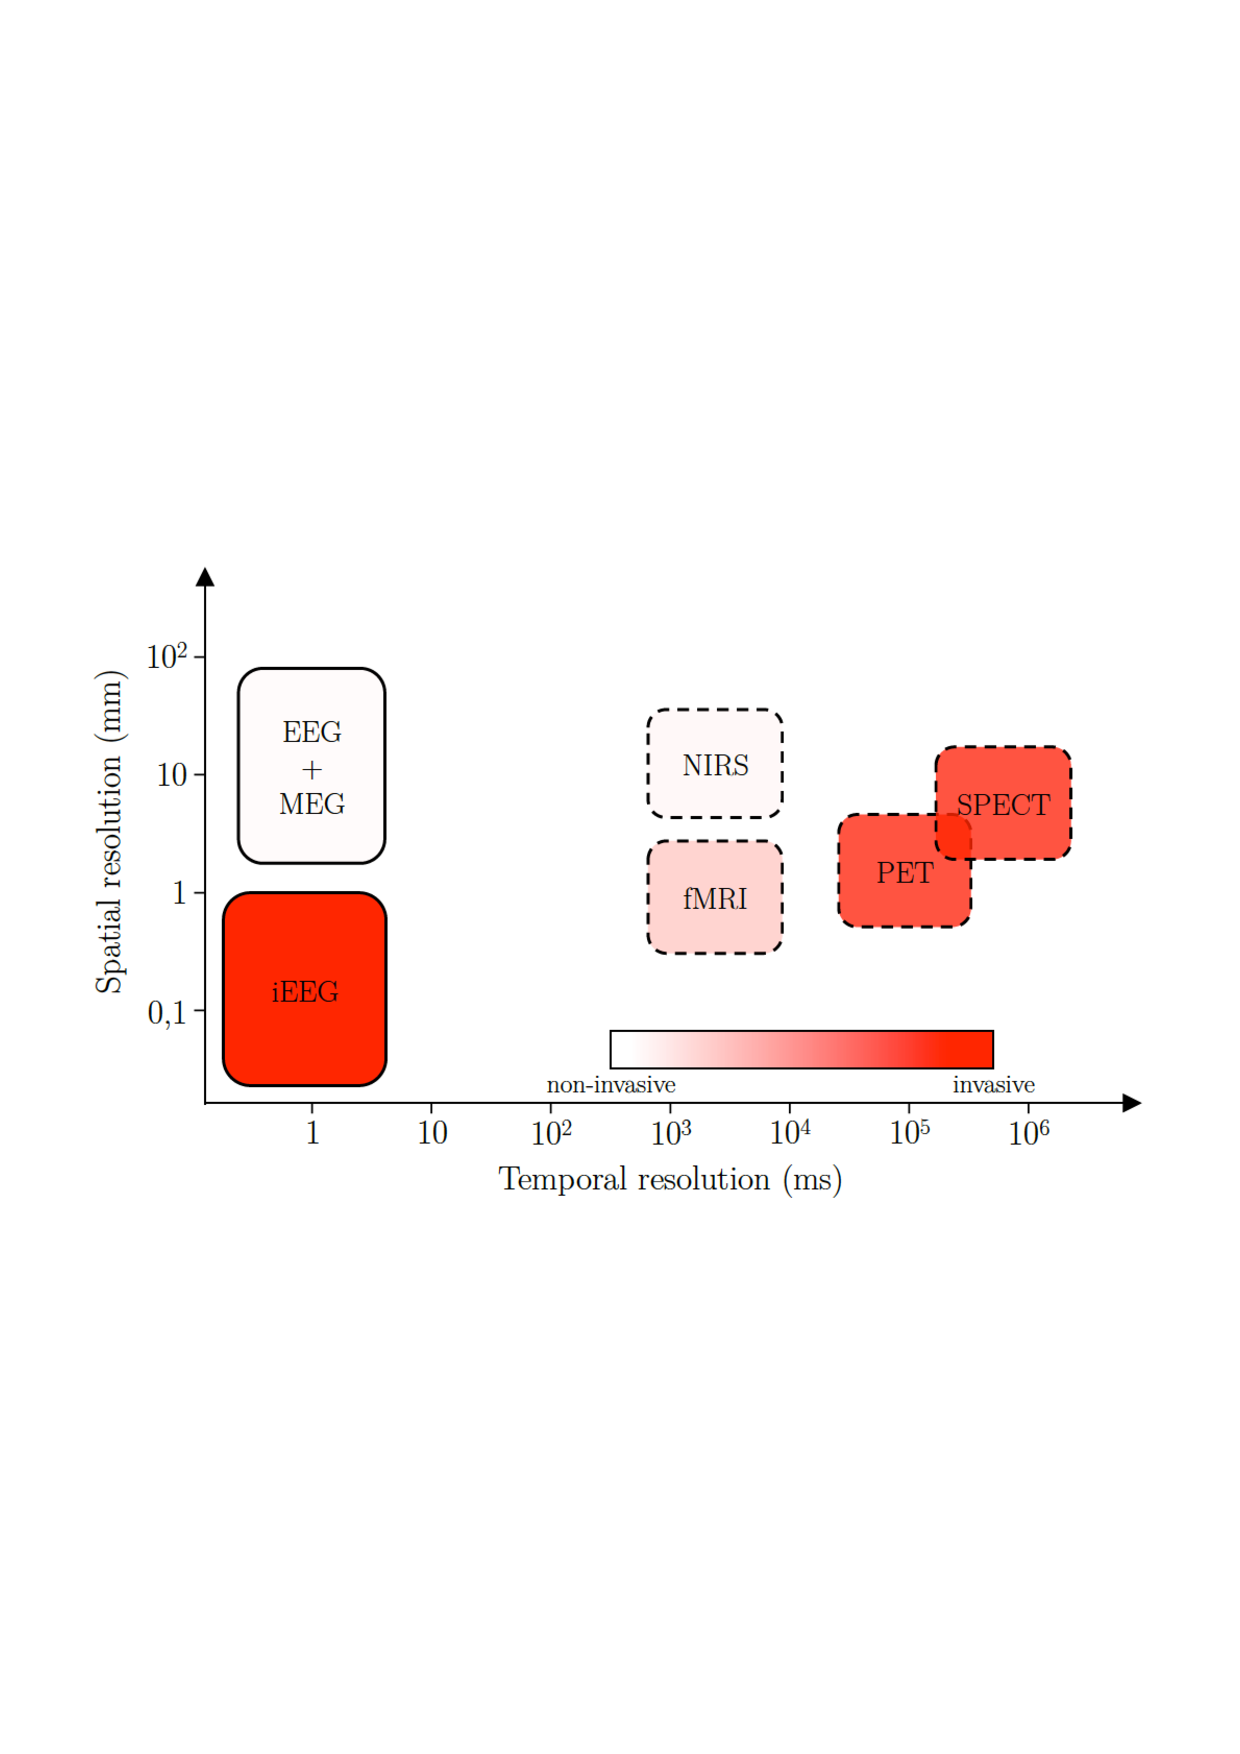
\includegraphics[trim={1cm 8cm 2cm 10cm},width=0.95\textwidth]{introduction/brain_imaging_techniques}
    \caption{Oveview on spatial and temporal resolutions of different functional neuroimaging methods. Direct approaches (EEG, iEEG, MEG) are indicated by solid boxes and indirect approaches (fMRI, NIRS, PET, and SPECT) by dashed boxes. The color of the boxes indicates the degree of invasiveness.
    }
    \label{fig:brain_imaging_techniques}
\end{figure}
 
Magnetoencephalography (MEG) and electroencephalography (EEG) are functional neuro-imaging techniques for mapping the brain activity. They respectively record the magnetic and electric fields produced by electrical currents naturally occurring in the brain within the neurons. They use an array of sensors positioned over the scalp that are extremely sensitive to minuscule changes in the magnetic field (measured by MEG) produced by small changes in the electrical activity (measured by EEG) within the brain. It is, therefore, a direct measurement of neural activity. MEG/EEG as a technique for investigating the neural function in the brain is not new but was originally pioneered in the late 1960s. However, it is only since the early 1990s, with the introduction of high density detector grids covering the whole head, that the full potential of MEG has begun to be realized. The biggest advantage of MEG and EEG compared to fMRI which is much more established in the neuroscience research is the time resolution. In fMRI, neural activation is indirectly measured via local changes in the level of blood oxygenation, a long time window is typically compressed in one measured brain volume. The other techniques mentioned in Figure~\ref{fig:brain_imaging_techniques} are also indirect functional brain imaging techniques.\\

Using very sensitive magnetometers/electrodes (sensors), MEG and EEG deliver insight into the brain activity with high temporal and good spatial resolution. They allow the measurements of the ongoing activity which describe the active brain sources' state at each millisecond. This problem of estimating the result of the measurements is called \textit{forward problem}. The bioelectromagnetic forward problem describes the relationship between a given neural activity in the brain and the observable MEG and EEG signals. Its solution models mathematically the neural activity, the volume conductor, and the measurement setup. It allows to link the scalp potentials and external fields given an internal current distribution by a stable and unique solution, which is thus a well-posed problem. \\

Its counterpart, the bioelectromagnetic \textit{inverse problem} consists in using the actual measurements to infer the parameters (locations, amplitude, orientations) giving the distribution of the neural generators. It is an ill-posed problem in the sense of Hadamard due to its non-uniqueness and high sensitivity to noise, which makes its solution unstable. The inverse problem is the so called $n \ll p$ problem in machine learning, where you have much more unknowns to estimate than the number of observations or variables. This problem has an infinite solution not only due to the small number of sensors (obervations $n$) present in the MEG and EEG. Actually, even if the MEG and EEG were measured simultaneously at infinitely many points over the head, the information will still be insufficient to uniquely compute the brain source distribution that generated the measured brain signals. This is due to the fact that there are different combinations of sources able to cause \textit{exactly} the same potential fields on the head. Thus, to infer the neural activity generating the data at the sensor level, different source reconstruction techniques can be applied, which typically employ a priori knowledge on the state of the brain activity in order to reduce the set of solutions to be a unique one.\\

In the past twenty years, several lines of research have emerged to tackle the problem. The most common approach widely used in clinical application is the equivalent current dipole (ECD), which assumes the underlying neural sources to be focal, as for epileptic study. The limitation of the dipole fitting technique is its non-linearity, which makes the reconstruction challenging. Also, difficulties to accurately estimating the correct number of dipoles in advance. \\

Unlike dipole fitting method, distributed source models divide the source space into a grid containing a large number of possible dipoles (ECDs). The reconstruction of the source space is done simultaneously over all ECDs, which is less challenging when having correlated sources. However due to the large number of dipoles, the corresponding regression problem is undertermined, and then requires regularization. The regularization will define the type of a priori one needs to put on the solution, such as structural information, spatio-temporal characteristics of the source estimate. The disadvantage of these models compared to dipole fitting is that the solution is smeared, meaning it is not focal so harder for interpretation.\\

Nevertheless, the sparsity in the solution can be promoted with a specific type of regularization to the regression model. The sparse models are actually the main interest of this thesis. They have been proposed in other fields of research and are widely used. In the signal processing literature, various signals can be defined as the linear combination of basis vectors, called \textit{atoms}. This technique is also known as compressed sensing. These atoms are defined in a fix overcomplete dictionary, the underlying motivation is that even though the observed signal is lying in a high-dimensional space, the actual signal is organized in a lower-dimensional space. This was used in the audio domain, specifically in the analysis of speech, sounds, and music, e.g. in order to classify a sound sample. The idea of sparse decomposition is also behind the JPEG2000 compression, which aims to keep only a few atoms best approximating the image. More in the image processing literature, the sparse models were used for denoising and image reconstruction (MRI,...). They are also linked to the dictionary learning literature, where one tries to learn a redundant and overcomplete dictionary, which is able to reconstruct a signal/image using a sparse setting.\\

\section*{Objective and scope}
%\textbf{Keywords:} Not only solve the IP but improve methods from the start to the end of the problem of source localization\\
%=> Sparse solutions (references), what people have been doing and how do we choosed to handle the problem\\
%=> Hyperparameter estimatio, to improve the tuning of the parameters which is important for solving the problem accurately.

In this thesis, I have been interested into the sparse models to reconstruct the source estimate for the MEG and EEG applications. Obtaining acceptable solutions, easy to interpret does not depend only on the a priori knownledge we impose, but several questions might be asked:
\begin{itemize}
\item How do we best fix the regularization to promote sparsity, in such a way to obtain interpretable source estimates?
\item How do we set the hyperparameters of the regression problem?
\item How do we quantify the uncertainty of these models?
\item How do we objectively compare the different state of the art solvers?
\end{itemize}
These points define the scope of this thesis. It tries to tackle firstly the problem of non-stationary sources, \textit{i.e.}, how to estimate a source that has a neuroscientific explanation as being active during a short time window only, when studying a longer window. This involves the formulation of the problem in the time-frequency domain, which needs to explicit the dictionary of the decomposition. Second, this thesis tries to find a way to automatically estimate the hyperparameter of the regression model to make comparison between solvers easier. Next step was to rewrite the problem as done by other communities: Bayesian formulation. This gave a way to bridge the gap between the variational and the Bayesian world by writing down their equivalence under a specific parametrization of the same problem. The advantage of the Bayesian formulation is the ability to investigate the posterior distribution, making a study of solution's uncertainty possible. This involves the presentation of Markov Chain Monte Carlo algorithms to sample from the posterior distribution. A third and last project of this thesis was to put together all the actual knowledge of source localization in MEG/EEG and have a complete study of their reconstruction on phantom dataset.

\section*{Contribution of the author}
This thesis presents novel approaches for source reconstruction in MEG/EEG. It can be divided into four main projects:
\begin{itemize}
\item The implementation of a widely known algorithm for MEG/EEG inverse problem, called Recursively Applied and projected (RAP) Music~\cite{mosher-leahy:1999}. The aim was to have a comparison with a state of the art sparse solver based on a non-convex regularization which promotes more sparsity by getting ride of all spurious sources. This work has been published in the \textbf{IEEE journal Transactions on Medical Imaging (TMI)}~\cite{strohmeier-etal:16}.

\item The improvement of a previous work of Daniel Strohmeier on source reconstruction in the time frequency domain, which resulted in the introduction of the TF-MxNE algorithm (Time-Frequency mixed-norm). The contribution tackles the problem of the choice of the dictionary where to decompose the data when working in the time-frequency domain. This consists on enabling the possibility to use combined dictionaries to make the algorithm able to find both transient and longer waveforms present in the brain signal. This work has been published in the IEEE conference \textbf{Pattern Recognition in NeuroImaging (PRNI)}~\cite{bekhti2016m}.

\item Different lines of research to solve the MEG/EEG inverse problem gave different formulations. The mostly used formulation in this thesis is a regularized regression model as done in most machine learning problems. With this type of models, one needs to find a good compromise between the term that tries to fit the data called the data fit and the term regularizing the problem which takes into account any assumption one has onto the problem. This compromise is controlled by an external parameter usually called hyperparameter. For a practical example, when using sparse regularization, if this hyperparameter is fixed to a small value, \textit{i.e.}, the regularization term is not as important as the data fit, so the resulting solution will not be sparse enough and vice versa. Thus, the second contribution of this thesis was then to find an automated way to estimate this hypermarameter under some conditions of the model. This work has been published in the \textbf{European Signal Processing Conference (EUSIPCO)}~\cite{bekhti_eusipco}.

\item The biggest drawback of the sparse solvers is the fact that it gives one solution without any estimation of variance or any kind of confidence intervals. Some other application areas make use of Bayesian inference, mainly because it allows the estimation of uncertainty and its quantification is paramount. Therefore, the third contribution of this thesis is to rewrite to problem as done by in a Bayesian world, and tries to bridge this formulation with what has been presented so far. This project shows that under some conditions, the Bayesian formulation and the variational one are equivalent. Then, it shows how we can get take advantage of the posterior distribution to extract uncertainty maps. This work has been submitted and is under review in the \textbf{journal Physics in Medicine \& Biology (PMB)}~\cite{bekhti_arxiv_pmb}.

\item The final project of this thesis is to test and validate our solvers and several other ones that are the mainly used at this day for neuroscience application. This is done on phantom dataset which is a simulated dataset with realistic environment as for a real humain brain. This work should be submitted soon to a journal paper.

\item An extra project on brain decoding is presented at the end of this thesis. This work presents a novel approach based on a ridge regression with a specific metric that takes into account ordered target. The approach is novel in terms of application to MEG data. This work has been submitted and is under review in the journal \textbf{Plos One}~\cite{Bekhti_bioarxiv}.

\item The implementation of some of the contribution is already on the MNE-Python package~\cite{MNE}, the others should also be integrated soon. Another minor contribution with a coworker's project is published in both \textbf{Pattern Recognition in NeuroImaging}~\cite{jas_autoreject_prni} and \textbf{Neuroimage}~\cite{jas_neuroimage}.
\end{itemize}

\section*{Structure of the thesis}
\begin{itemize}
\item \textbf{Chapter 1: Background and related work to the
M/EEG inverse problem}\\
This chapter defines the basics and the background needed for what will be presented in the rest of this thesis. It starts by giving the origin of the MEG and EEG recordings, \textit{i.e.}, what do the techniques really measure? It gives then more insight on the forward operator and how it is computed efficiently. At this stage, I present a full state of the art of inverse problems defining the three main approaches: beamforming or scanning techniques, image-based methods with distributed models, and sparse source models. Afterwards, I present some basics of time-frequency decomposition, and compare several dictionaries by giving their advantages. I finish this chapter by an optimization section, defining different ways to regularize the ill-posed problem and then how do we solve them. It also gives a comparison between several solvers.\\

\item \textbf{Chapter 2: Source localization with multi-scale dictionaries}\\
This chapter is dedicated to our first contribution, \textit{i.e.} solving the inverse problem in the time-frequency domain using a multi-scale dictionary. 
Source localization in the time-frequency domain has already been investigated using Gabor dictionary in a convex~\cite{Gramfort_Strohmeier_Haueisen_Hamalainen_Kowalski13} and a non-convex way~\cite{irTF-MxNE}. However, the choice of an optimal dictionary remains unsolved. Due to a mixture of signals, i.e. short transient signals (right after the stimulus onset) and slower brain waves, the choice of a single dictionary explaining simultaneously both signals types in a sparse way is difficult. This chapter introduces a method to improve the source estimation relying on a multi-scale dictionary, i.e. multiple dictionaries with different scales concatenated to fit short transients and slow waves at the same time. The benefits of this approach is shown in terms of reduced leakage (time courses mixture), temporal smoothness and detection of both signals types.

%Finally, the last chapter shows the experimental results obtained on simulated and on real MEG data. Then we discuss the achievements of this thesis and future work. 
%http://imaging.mrc-cbu.cam.ac.uk/meg/IntroEEGMEG

\item \textbf{Chapter 3: The Bayesian approach: Hierarchical Bayesian modeling}\\
This chapter gives the basic concepts of the Bayesian formulation of the MEG/EEG inverse problem. It also aims to explain the different jargon to link the variational and the Bayesian definitions. This ends up at defining an equivalence between the two communities under some conditions, while taking advantage of the Bayesian formulation which enables to study the multiple modes of the posterior distribution. The modes of the posterior will define several possible solutions to the inverse problem, allowing then the obtention of uncertainty maps of the source estimates. 

\item \textbf{Chapter 4: Benchmarking on phantom datasets}\\
This chapter is a validation chapter on phantom dataset. Phantom data is a dataset obtained by measuring the MEG/EEG activity with a humain skull phantom head. All real aspects of a head are simulated to generate the same conductivity which is due with a real skull. The dataset shown in this chapter has 4 simulated dipoles at different depth. With the knownledge of the groundtruth, this chapter investigates the efficiency of each solver in terms of source localization, orientation and amplitudes.

\item \textbf{Chapter 5: Decoding visual motion from MEG}\\
This chapter illustrates an extra project outside of the inverse problem topic. It is based on an application of machine learning to neuroscience. The aim was to develop an efficient approach to decode brain activity recorded with MEG while participants discriminated the coherence of two intermingled clouds of dots.
\end{itemize}

\newpage
\section*{Publications of the author}
\textbf{Peer-reviewed journal papers:}
\begin{itemize}
\item \textbf{Y. bekhti}, and A. Gramfort, "Validation of dipole localization using phantom data in MEG source imaging," in preparation.
\item \textbf{Y. Bekhti}, F. Lucka, J. Salmon, and A. Gramfort, "A hierarchical Bayesian perspective on majorization-minimization for non-convex sparse regression: application to M/EEG source imaging," ArXiv preprint, (submitted).
\item \textbf{Y. Bekhti}, A. Gramfort, N. Zilber, and V. van Wassenhove, "Decoding the categorization of visual motion with magnetoencephalography," Plos One, (submitted).
\item D. Strohmeier, \textbf{Y. Bekhti}, J. Haueisen, and A. Gramfort, "The iterative reweighted Mixed-Norm Estimate for spatio-temporal MEG/EEG source reconstruction," IEEE Transactions on Medical Imaging, vol. 35, no. 10, pp. 2218-2228, 2016.
\item M. Jas, D.A. Engemann, \textbf{Y. Bekhti}, F. Raimondo, and A. Gramfort, "Autoreject: Automated artifact rejection for MEG and EEG data," NeuroImage, vol. 159, pp. 417-429, 2016.
\end{itemize}

\textbf{Peer-reviewed conference papers:}
\begin{itemize}
\item \textbf{Y. Bekhti}, R. Badeau, and A. Gramfort, "Hyperparameter estimation in maximum a posteriori regression using group sparsity with an application to brain imaging," Signal Processing Conference (EUSIPCO), pp. 246-250, 2017.
\item \textbf{Y. Bekhti}, D. Strohmeiery, M. Jas, R. Badeau, and A. Gramfort, "M/EEG source localization with multi-scale time-frequency dictionaries," International workshop on Pattern Recognition in NeuroImaging (PRNI), pp. 1-4, 2016.
\item M. Jas, D.A. Engemann, F. Raimondo, \textbf{Y. Bekhti}, and A Gramfort, "Automated rejection and repair of bad trials in MEG/EEG", International workshop on Pattern Recognition in NeuroImaging (PRNI), pp. 1-4, 2016.
\end{itemize}


%----------------------------------------------------------------------------------------
%	THESIS CONTENT - CHAPTERS
%----------------------------------------------------------------------------------------

\mainmatter % Begin numeric (1,2,3...) page numbering

\pagestyle{thesis} % Return the page headers back to the "thesis" style

% Include the chapters of the thesis as separate files from the Chapters folder
% Uncomment the lines as you write the chapters
\numberwithin{figure}{section}

% Chapter 1

\chapter{Background and work related to the M/EEG inverse problem} % Main chapter title
\label{chapter:background} % For referencing the chapter elsewhere, use \ref{Chapter1} 
\noindent\makebox[\linewidth]{\rule{0.75\paperwidth}{0.4pt}}
\noindent\makebox[\linewidth]{\rule{0.75\paperwidth}{0.4pt}}

\localtableofcontents % local toc

\noindent\makebox[\linewidth]{\rule{0.75\paperwidth}{0.4pt}}
\noindent\makebox[\linewidth]{\rule{0.75\paperwidth}{0.4pt}}

\newpage
%----------------------------------------------------------------------------------------

% Define some commands to keep the formatting separated from the content 
\newcommand{\keyword}[1]{\textbf{#1}}
\newcommand{\tabhead}[1]{\textbf{#1}}
\newcommand{\code}[1]{\texttt{#1}}
\newcommand{\file}[1]{\texttt{\bfseries#1}}
\newcommand{\option}[1]{\texttt{\itshape#1}}


%--------- Signal sources of MEEG recording-----------------------------------------------
\section{Signal sources of MEG and EEG recordings}
%Measuring weak MEG/EEG signals in the background of strong environmental noise, having a noise level of several orders of magnitude larger than the MEG/EEG signals, is a challenging task. 
At the cellular level of the brain, its nervous system is defined by the presence of a special type of neural cells. Despite the apparent simplicity in the structure of the neural cell, the biophysics of the neural current flow relies on a complex network of billions of cells, neurons and glial cells~\cite{baillet2001electromagnetic, hodgkin1964conduction}. Neurons are nerve cells that transmit nerve signals to and from the brain. They are about 100 billions neurons. The neuron consists of a cell body (or soma) with branching dentrites (signal receivers). They send these signals in the form of electrochemical waves traveling along thin fibers called axons, which cause chemicals called neurotransmitters to be released at junctions called synapses. A cell that receives a synaptic signal from a neuron may be excited, inhibited, or otherwise modulated. At a synapse, the cell that sends signals is called presynaptic, and the cell that receives signals is called postsynaptic.\\

Every neuron maintains a voltage gradient across its membrane, due to metabolically driven differences in ions of sodium, potassium, chloride and calcium within the cell, each of which has a different charge. If the voltage changes significantly, an electro-chemical pulse called an action potential (or nerve impulse) is generated. This electrical activity can be measured and displayed as a waveform called brain wave or brain rhythm. This pulse travels rapidly along the cell's axon, and is transferred across a synapse to a neighbouring neuron, which receives it through its feathery dendrites. Each individual neuron can form thousands of links with other neurons in this way, giving a typical brain well over 100 trillion synapses (up to 1,000 trillion, by some estimates).\\

Roughly, when a neuron is excited by other —and possibly remotely located— neurons via an afferent volley of action potentials, \ac{EPSP}s are generated at its apical dendritic tree. The apical dendritic membrane becomes transiently depolarized and consequently extracellularly electronegative with respect to the cell soma and the basal dendrites. This potential difference causes a current to flow through the volume conductor from the nonexcited membrane of the soma and basal dendrites to the apical dendritic tree sustaining the EPSPs~\cite{gloor1985neuronal}.
Some of the current takes the shortest route between the source and the sink by traveling within the dendritic trunk. Conservation of electric charges imposes that the current loop be closed with extracellular currents flowing even through the most distant part of the volume conductor. Intracellular currents are commonly called primary currents, while extracellular currents are known as secondary, return, or volume currents.\\

Both primary and secondary currents contribute to magnetic fields outside the head and to electric scalp potentials, but spatially structured arrangements of cells are of crucial importance to the superposition of neural currents such that they produce measurable fields. Tens of thousands of synchronously activated large pyramidal cortical neurons are thus believed to be the main MEG and EEG generators because of the coherent distribution of their large dendritic trunks locally oriented in parallel, and pointing perpendicularly to the cortical surface~\cite{nunez2000relationship}. The currents associated with the EPSPs generated among their dendrites are believed to be at the source of most of the signals detected in MEG and EEG because they typically last longer than the rapidly firing action potentials traveling along the axons of excited neurons~\cite{nunez2006electric}. %Indeed, calculations such as those shown in~\cite{hamalainen1993magnetoencephalography} suggest each synapse along a dendrite may contribute as little as a 20 fA-m current source, probably too small to measure in MEG/EEG. Empirical observations instead suggest we are seeing sources on the order of 10 nA-m, and hence the cumulative summation of millions of synaptic junctions in a relatively small region. Nominal calculations of neuronal density and cortical thickness suggest that the cortex has a macro-cellular current density on the order of 100 nA/mm2.\\

\begin{figure}
	\centering
	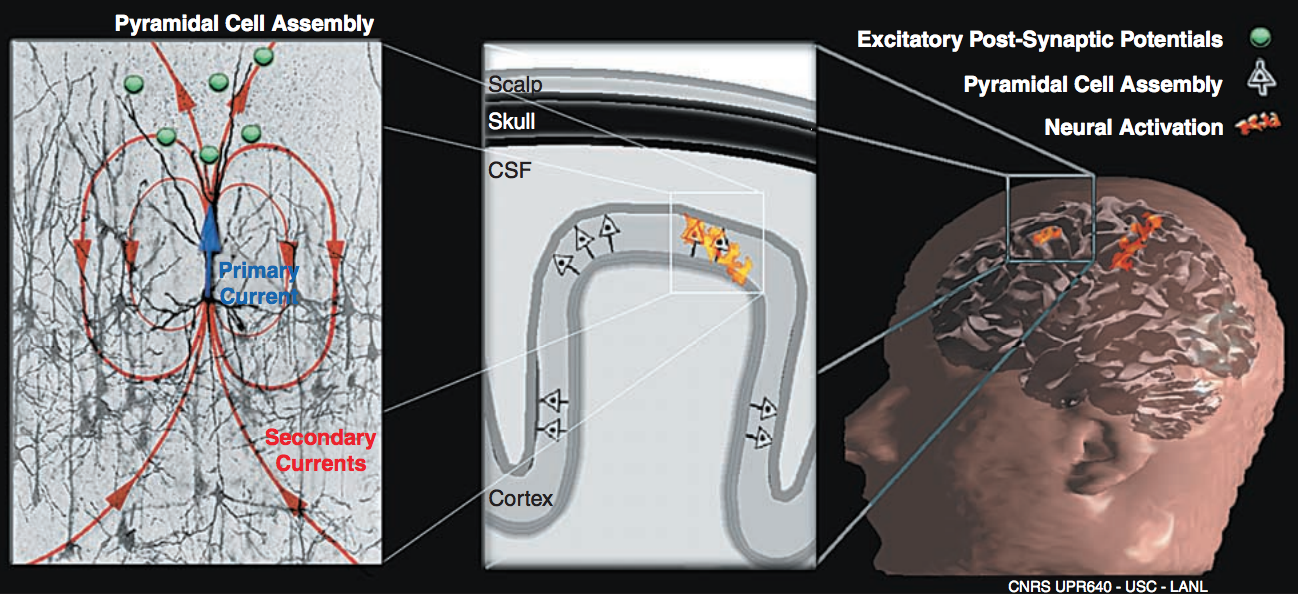
\includegraphics[width=0.95\textwidth]{background/network_cortical_neural_cells}
    \caption{Networks of cortical neural cell assemblies are the main generators of MEG/EEG signals. Left: Excitatory postsynaptic potentials (EPSPs) are generated at the apical dendritic tree of a cortical pyramidal cell and trigger the generation of a current that flows through the volume conductor from the non-excited membrane of the soma and basal dendrites to the apical dendritic tree sustaining the EPSPs. Center:  Large cortical pyramidal nerve cells are organized in macro-assemblies with their dendrites normally oriented to the local cortical surface. This spatial arrangement
and the simultaneous activation of a large population of these cells contribute to the spatio-temporal superposition of the elemental activity of every cell, resulting in a current flow that generates detectable EEG and MEG signals. Right: Functional networks made of these cortical cell assemblies and distributed at possibly mutliple brain locations are thus the putative main generators of MEG and EEG signals. The origin of this image is~\cite{baillet2001electromagnetic}.
    }
    \label{fig:network_cortical_neural_cells}
\end{figure}

MEG and EEG are non-invasive functional imaging techniques for analyzing the neuronal activity on a macroscopic scale. In contrast to indirect neuroimaging modalities, MEG and EEG signals derive from the net effect of ionic currents flowing in the dendrites of neurons during synaptic transmission. In accordance with Maxwell's equations, any electrical current will produce a magnetic field, and it is this field that is measured. The measurement principle of MEG and EEG is illustrated in Figure~\ref{fig:meg_eeg_principle}.\\

The neuronal activity captured by MEG is not, as perhaps expected, generated by the (too brief) axonal action potentials of pyramidal cells, but rather by the net contributions of excitatory and inhibitory dendritic postsynaptic potentials. This current flow through the apical dendrites (represented as a ‘dipole’) generates a magnetic field that projects radially; thus, MEG excels at detecting dipoles arranged in a tangential orientation to the skull. Fortunately, the extensively folded sulci of the human cortex promote that orientation for the majority of cortical microcolumns. However, MEG is less sensitive to deeper (including subcortical) sources, as the magnetic field change decreases rapidly with distance.\\

\begin{figure}
	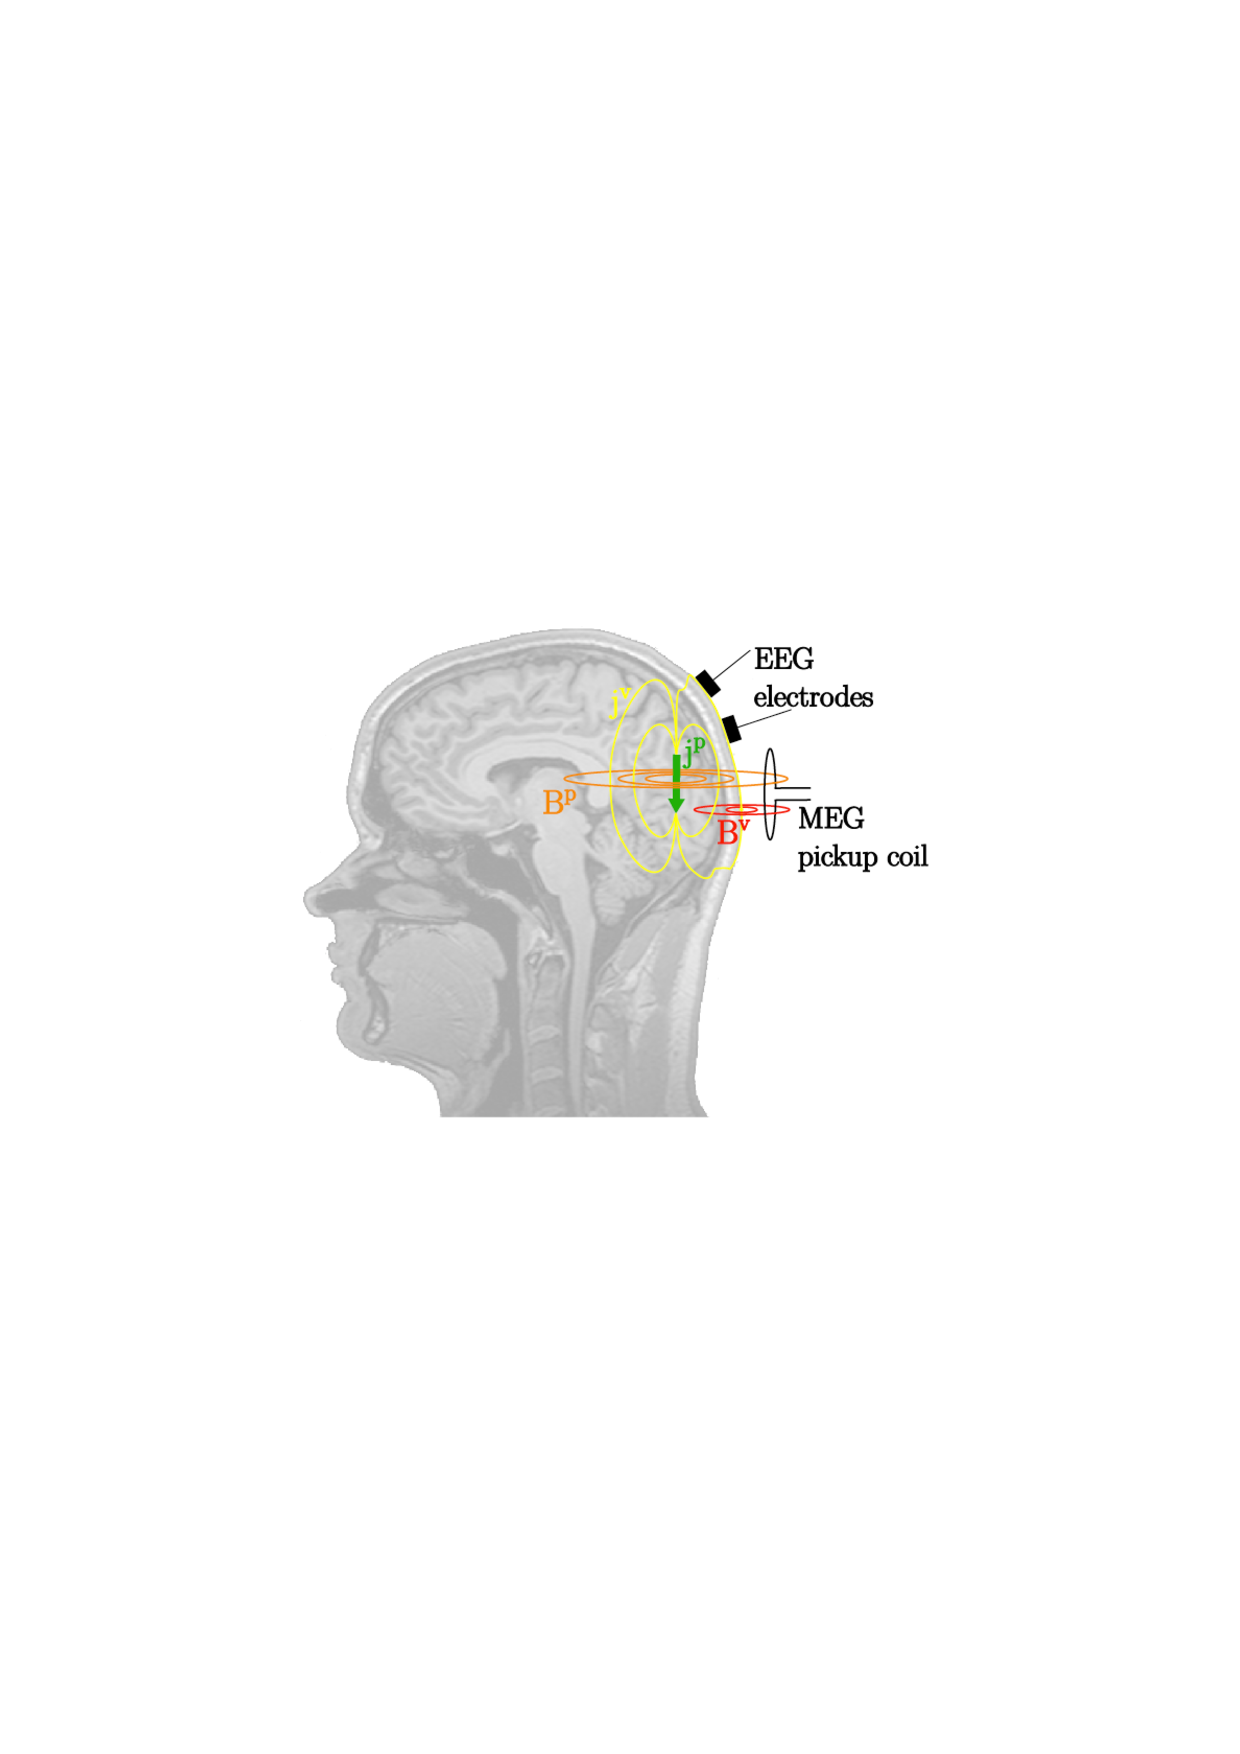
\includegraphics[trim={1cm 10cm 2cm 10cm},width=0.95\textwidth]{background/meg_eeg_principle}
    \caption{Simplified model of the measuring principle of MEG and EEG. The EEG measures the difference of the electric potential between the EEG electrode and a reference due to volume currents generated by primary currents in the brain. The
MEG captures the magnetic field generated by both primary and volume currents.
    }
    \label{fig:meg_eeg_principle}
\end{figure}

In 1969, the journey to understand the electrical potentials of the brain took an interesting and fruitful detour when David Cohen, a physicist working at MIT, became the first to confidently measure the incredibly tiny magnetic fields produced by the heart's electrical signals. To do this, he constructed a shielded room, blocking interference from the overwhelming magnetic fields generated by earth itself and by other electrical devices in the vicinity, effectively closing the door on a cacophony of voices to carefully listen to a slight whisper. His shielding technique became central to the advent of MEG, which measures the yet even quieter magnetic fields generated by the brain's electrical activity.\\ % XXX add ref

This approach to record the brain's magnetic fields, rather than the electrical potentials themselves, was advanced even further by James Zimmerman and others working at the Ford Motor Company, where they developed the SQUID, a Superconducting QUantum Interference Device. A SQUID is an extremely sensitive magnetometer, operating on the principles of quantum physics, which is able to detect precisely those very tiny magnetic fields produced by the brain. To appreciate the contributions of magnetic shielding and SQUIDs to magnetoencephalography, consider that the earth's magnetic field, the one acting on your compass needle, is at least 200 million times the strength of the fields generated by your brain trying to read that very same compass.\\

On the other hand, the EEG measures the electric potential difference between the EEG electrode and a reference on the scalp associated with primary currents in the brain. These electric potential differences, which are in the range of a few microvolts, are recorded using amplifiers with high open-loop gain, common-mode rejection ratio, and input impedance. The first human EEG recording was done by Hans Berger in 1924.\\

MEG and EEG can be recorded simultaneously and reveal complementary properties of the electrical fields. Although the signals of EEG and MEG are generated by the same sources (electrical currents in the brain), they are both sensitive to different aspects of these sources. This could be compared to viewing the shadows of the same object from two different angles; combining the two recordings usually leads to better source estimation~\cite{malmivuo2012comparison,sharon2007advantage,aydin2015combined}.

%--------- Forward model -------------------------------------------------------------------
\section{The forward model}
The bioelectromagnetic forward problem describes the relationship between a given neural activity in the brain and the observable MEG and EEG signals. We assume the electric current (denoted by $\vec{j}_t(\vec{r})$) at any position (denoted by $\vec{r}$ in the head is known at arbitrary time $t$. The magnetic field or the scalp voltage detected by one sensor can be modeled as an integration or a linearly weighted combination of the currents at all positions, using Maxwell's equations under a reasonable head model that describes the shape, the electrical conductivity and the permeability of various tissues~\cite{hamalainen1993magnetoencephalography,mosher1999eeg}.

\subsection*{Maxwell's equations}
We consider the head as a finite three-dimensional volume conductor, non magnetic. The quasi-static approximation of Maxwell's equations are a set of partial differential equations forming the foundation of classical electromagnetism. We denote by $\mathbf{E}$ the electric field, $\mathbf{B}$ the magnetic field, $\mathbf{J}$ the current density, and $\rho$ the charge density.

\begin{center}
$\left\{
\begin{array}{l}
  \nabla . \mathbf{E} = \frac{\rho}{\epsilon} \\
  \nabla \times \mathbf{E} = \frac{-\partial \mathbf{B}}{\partial t} \\
  \nabla \cdot \mathbf{B} = 0 \\
  \nabla \times \mathbf{B} = \mu_0 (\mathbf{J} + \epsilon\frac{\partial \mathbf{E}}{\partial t})
\end{array}
\right.$
\end{center}

For the biological signals of interest in MEG/EEG, the time-derivatives of the associated electric and magnetic fields are sufficiently small to be ignored in Maxwell’s equations. Recent discussions and details of this quasi-static approximation can be found in\cite{hamalainen1993magnetoencephalography,tripp1983physical,heller1992brain}.\\

The propagation of the electric potentials and magnetic field measured by EEG and MEG suffers from no temporal delay, meaning that the recording is instantaneous. Let us note $\mathbf{M}\in\RR^{N\times T}$ the measurement matrix of MEG/EEG, $\mathbf{G}\in\RR^{N\times SO}$ the design matrix (leadfield or gain matrix~\cite{h1994}) with $S$ source locations in the brain and $O$ number of orientations (1 or 3). One has:
\begin{equation}
\mathbf{M} = \mathbf{GX}+\mathbf{E}
\end{equation} \label{eq:meeg_ip}
\noindent From now on, $\mathbf{E}$ denotes an additive white Gaussian noise. Equation~\eqref{eq:meeg_ip} is linear not by assumption but by guarantee from Maxwell's equations.\\

If the source orientation is set a priori, \textit{e.g.}, by using the cortical constraint assuming sources to be oriented perpendicularly to the cortical surface~\cite{Dale:1993} (O = 1), a single dipole with unit norm per source location is used to compute the gain matrix $\mathbf{G}\in\RR^{S\times T}$. To allow for arbitrary dipole orientations, the dipole moment per location is represented by a linear combination of O perpendicular unit dipoles. An orthogonal dipole triplet is commonly applied (O = 3). Due to the low sensitivity of MEG to radial sources, the radial component per source location is sometimes neglected (O = 2). The gain matrix $\mathbf{G}$ is generated by solving the MEG/EEG forward problem for each dipole separately and by appending the results column-wise. Hence, each column of the gain matrix provides information on the topography in the sensor space generated by the activity of a specific unit dipole, while each row reflects the sensitivity of a specific sensor to all unit dipoles in the model.

\subsection*{Spherical head models}
A very common approximation in the forward modeling consists in assuming that the head is a set of nested concentric spheres, each corresponding to a layer with homogeneous and isotropic conductivity (Figure~\ref{fig:sphere_align}). Typically, the head is represented by three to five regions, \textit{e.g.}, scalp, skull, cerebrospinal fluid, gray matter, and white matter, and that the conductivity is constant and isotropic within these regions. The gradient of the conductivity is therefore zero except at the surfaces between regions. Computable analytic solutions exist for both MEG and EEG forward problems.\\

A very practical formulation of the EEG and MEG field kernels has been presented by Mosher~\cite{mosher1999eeg}, that only requires vectors expressed in their Cartesian form. For MEG, since the magnetic permeability does not change across layers (and does not change much from the vacuum) and no current exists outside the head (where the sensors are located), the full magnetic field outside a set of concentric spheres can be calculated without explicit consideration of the volume currents. Therefore, the MEG spherical model does not require specifying (or assuming) the number of and the radius ratios between the spherical layers.\\

\begin{figure}
\centering
	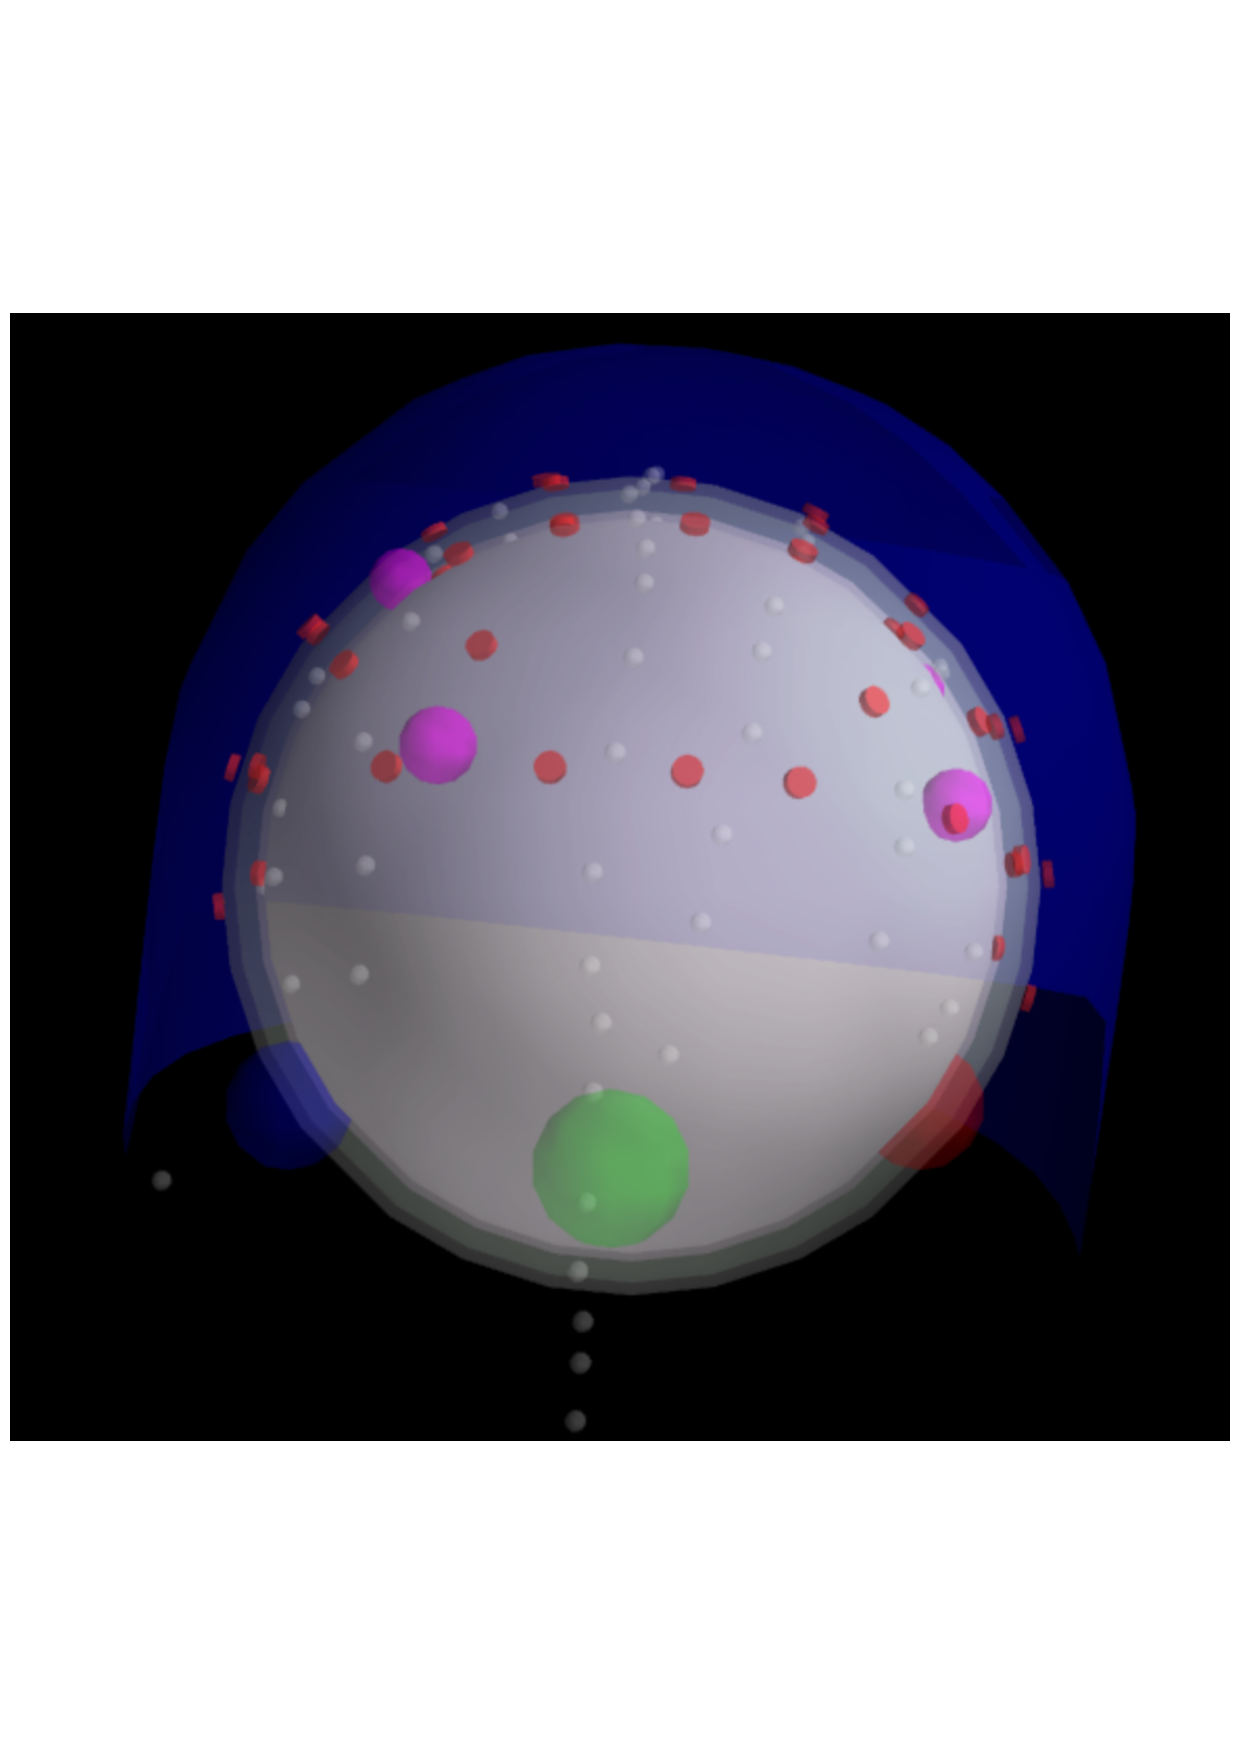
\includegraphics[trim={0cm 5cm 0cm 5cm},width=0.6\textwidth]{background/sphere_align}
    \caption{The alignment of a spherical model with three layers and the sensors. The spheres are shown in grey, the sensors space in blue, and the dots to align in order to put the spheres modeling the head and the sensors in a common coordinate system.}
	\label{fig:sphere_align}
\end{figure}

For EEG, the number and radii of the spherical layers are to be specified. Nonetheless, previous empirical work on closed-form approximations by Berg and Scherg~\cite{berg1994fast} and related theoretical studies by Zhang~\cite{zhang1995fast} have gathered a valid and convenient method for approximating an EEG field kernel from a multi-layer spherical model as the weighted sum of three kernels from a single-layer spherical model applied to a modified source configuration. The optimal values of the "Berg parameters" (Eccentricity and Magnitude) in this approximation depend on the layer radii and conductivities.

\subsection*{Realistic head models}
A more realistic head model requires that the real geometry and conductivity of the head layers be taken into account as much as possible (Figure~\ref{fig:head_model}). For real (non-spherical) geometry and conductivity fields, numerical solutions for Maxwell's equations are to be computed.\\
\begin{figure}
\centering
	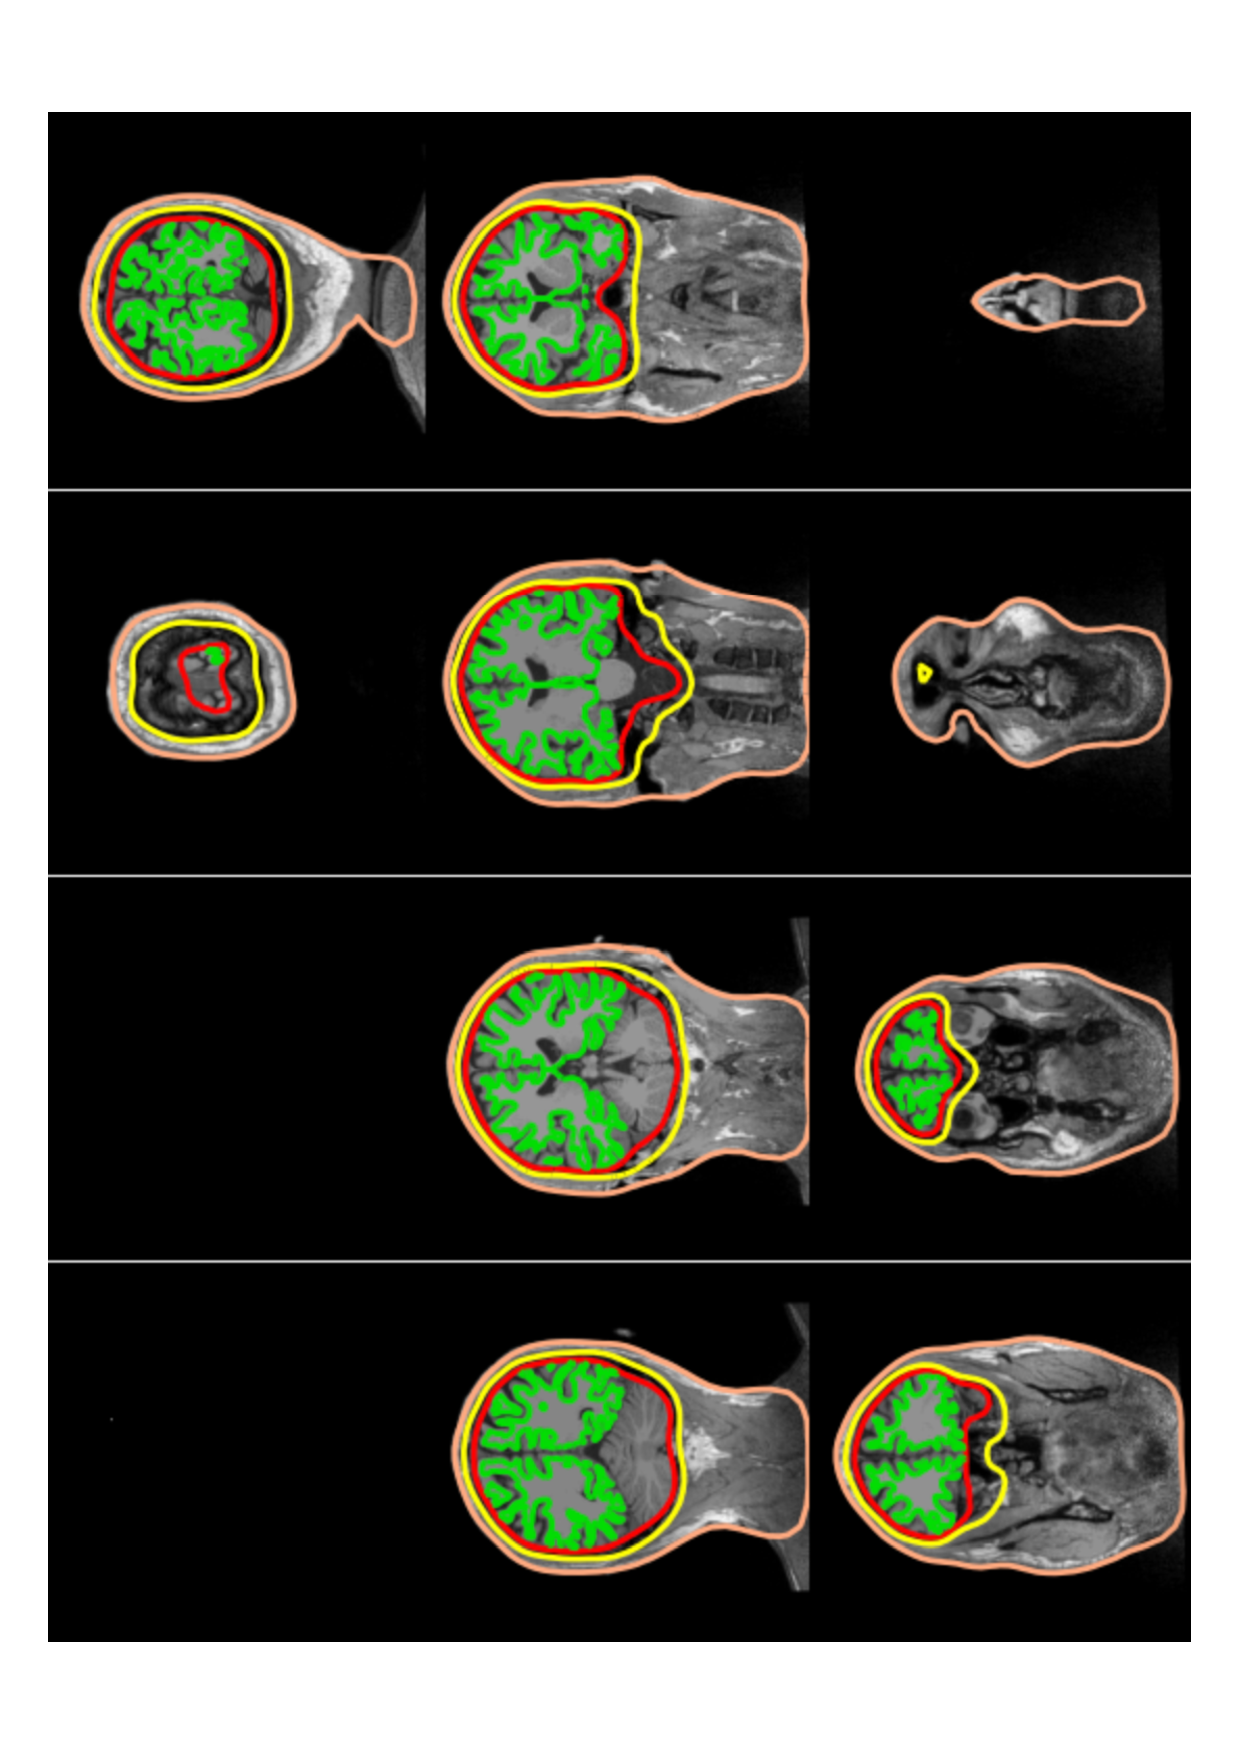
\includegraphics[angle=270,width=0.95\textwidth]{background/head_model}
    \caption{The head model: the BEM surfaces containing the three layers (inner skull, outer skull, and skin).}
	\label{fig:head_model}
\end{figure}
Assuming a piecewise constant distribution of the conductivity field, approximate, yet efficient and accurate, numeric solutions can be obtained for a realistically shaped head model using the so-called \ac{bem}. For BEM solutions, an MRI-based simplified description of the geometry is needed for computing the lead fields, and this can be provided in terms of (strictly) nested and closed surfaces corresponding to the boundaries separating the main tissue compartments (also called layers).
In practice, BEM solutions will only require to set a few conductivity parameters (one per tissue), and to specify a few triangular meshes, as can be obtained, \textit{e.g.}, with 3D volume segmentation tools from anatomical MRI data, each representing a separate interface between layers. \\

% http://leonidzhukov.net/content/eeg_meg_physics/node1.html
% http://www.brainvoyager.com/bvqx/doc/UsersGuide/EMEGSuite/EEGAndMEGForwardModels.html

%--------- MEEG inverse problem ------------------------------------------------------------
\section{The MEG/EEG Inverse problem}
An important question in the MEG/EEG community since the neuronal activity is measured at a sensor-level distributed over the head, is "how to recover the brain region(s) involved in producing the measured activity?". This is the so-called bio-electromagnetic inverse problem which is ill-posed in contrast to the forward problem. The uniqueness of the inverse problem solution is due to the fact that MEG/EEG signals can be produced by an infinite number of source configurations. Thus, to identify a stable and a unique solution among all of these infinite configurations, constraints need to be set. The constraints are chosen depending on the assumptions or a priori knowledge based on the characteristics of the source distributions, \textit{e.g.}, spatial and/or temporal characteristics of the neural activity. The source reconstruction techniques can be in general categorized as parametric (Section~\ref{section_dipfit}), scanning (Section~\ref{section_scanning}), and probabilistic methods (Section~\ref{section_distributed}).

\subsection{Parametric models: \textit{dipole fitting}} \label{section_dipfit}
Parametric methods model the problem as a small number of sources defined by their location, orientation and the strengths of the current sources that generate the MEG/EEG measurements.\\
The most common parametric method is the dipole fitting approaches \cite{scherg1985two,mosher1992multiple,scherg1990fundamentals}. It assumes that the measured data have been produced by a small number of active brain regions that can each be modeled using an equivalent current dipole (ECD). These algorithms minimize a data-fit cost function such as the Frobenius norm of the residual, and they estimate five non-linear parameters per dipole: the 3D $(x,y,z)$ position, and the two angles to define the dipole orientation. The main limitation of these methods is that they cannot be used when complex cognitive tasks are performed. This is due to the fact that the optimization problem to be solved is not linear, which implies that it gets easily trapped in local minima as soon as one tries to localize more than two dipoles. Furthermore, the number of dipoles to be estimated is not known and then needs to be set in advance. 

\subsection{Scanning methods: \textit{beamforming \& MUSIC}} \label{section_scanning}
Scanning methods, \textit{a.k.a.} beamforming, use a discrete grid to search for optimal dipole positions throughout the source space~\cite{hillebrand2005new,mosher99mulsigclassif,scherg1985two}. An estimator of the contribution of each source location to the data can be derived either via spatial filtering or signal classification settings. The simplest spatial filter is \textit{a matched filter} which uses the normalized columns of the gain matrix for spatial filtering, but the most common one is the linearly constrained minimum variance (LCMV) beamformer \cite{van1997localization}.\\
%and multiple signal classification (MUSIC) methods and their variants.\\
LCMV performs a spatial filtering on data to discriminate between signals originating from a location of interest and those coming from elsewhere, and limits the influence of the noise. In practice, it implies that the measurement matrix is multiplied by a weighting matrix. The weighting matrix should let pass signals coming from the location of interest, while attenuating signals from elsewhere. LCMV determines the weighting matrix by minimizing the output power of a filter under a constraint that its gain (forward operator) is unity at the location of interest. An attractive feature of beamforming is that it does not require any assumption on the number of the underlying sources. However it makes the strong assumption that the activations of the different sources are uncorrelated, which is not necessarily the case. An alternative to LCMV which integrates some information related to the experimental paradigms is called Synthetic Aperture Magnetometry (SAM) \cite{vrba2001signal}. Beamforming can also be applied in the frequency domain using the Dynamic Imaging of Coherent Sources (DICS) \cite{gross2001dynamic}.
%The difference between beamformers is the constraint for estimating the weighting matrix. LCMV determines the weighting matrix by minimizing the output power of a filter under a constraint that its gain is unity at the location of interest. The limitation of this approach is that signal cancellation may occur, when different sources are correlated (Baillet et al. 2001). Another beamformer often used is Synthetic Aperture Magnetometry (SAM) (Vrba and Robinson, 2001).\\

Alternatives to beamformers are methods based on signal classification using subspace decompositions. The MUltiple SIgnal Classification (MUSIC) is a widely known signal processing technique that was first applied to EEG data by \textit{Mosher} \cite{mosher1992multiple}. The primary assumptions for this method are that the dipolar time series are mutually linearly independent. 
MUSIC is based on a singular value decomposition (SVD) of the measurement data, which results in orthogonal basis vectors and singular values. Any true source localization will have a lead field (forward) vector which lies in the signal subspace computed with the SVD. MUSIC scans the brain space for source locations that satisfy this condition. The lead field vector at every candidate dipole location is systematically projected onto the signal subspace. The dipole source locations with the largest projections on the signal subspace are the active sources \cite{mosher1992multiple,mosher1999source}. However, MUSIC suffers from some problems. Firstly, when the noise present in the data is correlated across channels, MUSIC can produce larger errors in the dipole localization than would have been observed with uncorrelated noise of the same power. Another problem is the detection of multiple MUSIC peaks in a 3D space of the head, each of which may correspond to a different ECD. A related problem is to determine which peaks are truly indicative of a dipolar source rather than a local minimum in the error function \cite{mosher1999source}.

The latter problem is solved in an extended version of MUSIC, Recursively Applied and Projected (RAP)-MUSIC, by recursive estimation of multiple sources \cite{mosher1997source,mosher1999source}. In other words, it consists in applying MUSIC successively after removing the contribution of the previously identified sources. Such as matching pursuit algorithms are used for sparse signal decomposition over dictionary of atoms \cite{mallat1993matching}, the RAP-MUSIC method adopts a greedy strategy to select the relevant dipoles in a dictionary of sources. The implementation of RAP-MUSIC and its comparison with another solver was the first contribution of this thesis \cite{strohmeier-etal:16}.
%Recently, an alternative method was developed called FINES (Xu, et al., 2004). This method is able to localize closely spaced correlated sources.

\subsection{Probabilistic modeling: \textit{distributed sources \& Bayesian approaches}} \label{section_distributed}
Distributed source localization estimates the amplitudes of a dense set of dipoles distributed at fixed locations within the head surface or volume. These methods are based on the reconstruction of the brain electric activity in each point of a 3D grid of solution points, the number of points being much larger that the number of electrodes on the scalp. Each solution point is considered as a possible location of a current source, thus there is no a priori assumption on the number of dipoles in the brain.
When orientations are fixed and only the amplitudes of the sources are estimated, the forward problem results in a regression formulation.

The MEG/EEG inverse problem with distributed source models leads to a regularized regression problem. The widely known method \textit{Minimum Norm Estimate} (MNE) minimizes the $\ell_2$-norm \cite{hamalainen1994interpreting}. %The standard MNE is given in Eq.\ref{eq_thikonov}.
MNE has been very attractive due to the fact that the inverse solution is given by a simple matrix multiplication as $\ell_2$-based methods have closed-form solutions:

\begin{equation}\label{eq_MNE}
\mathbf{X}^\star = \argmin_{\mathbf{X}\in\RR^{SO\times T}} \|\mathbf{M}-\mathbf{GX}\|_{Fro}^2 + \lambda\|\mathbf{X}\|_2^2 \hspace{10pt} \mathrm{with} \hspace{10pt} \lambda > 0
\end{equation}

However, the choice of the $\lambda$ parameter as the trade-off between data fit and regularization is sometimes tricky, because it depends on the data since $\lambda$ is related to the noise level present in the measurement. $\lambda$ is most of the time chosen with a cross-validation strategy to find the optimal value in the machine learning community. While in the MEG/EEG world, it is mostly tuned by hand.

When applying a minimum-norm estimate as in Equation~\eqref{eq_MNE}, all the sources are penalized equivalently. This approach introduces bias over sources which are far from the sensors. Indeed sources which are close to the sensors have a higher forward field. Those sources are called superficial sources, and this bias is often known as the depth bias~\cite{pascual1999review}. This led to the introduction of the Weighted Minimum Norm (WMN) estimate \cite{lin2006assessing}, which downweights the dipoles in the head that are closer to the surface. 

\begin{equation}\label{eq_wMNE}
\mathbf{X}^\star = \argmin_{\mathbf{X}\in\RR^{SO\times T}} \|\mathbf{M}-\mathbf{GX}\|_{Fro}^2 + \lambda\|\mathbf{WX}\|_2^2 \hspace{10pt} \mathrm{with} \hspace{10pt} \lambda > 0
\end{equation}

$\mathbf{W}$ is a weighting matrix, which represents a priori knowledge on the source covariance. Assigning a higher variance to a deep sources is a standard approach to reduce the depth bias in MEG/EEG source imaging~\cite{lin2006assessing, Gramfort_Strohmeier_Haueisen_Hamalainen_Kowalski13,haufe2008combining, haufe2011large,huang2014meg,palmero2007swloreta}. A common practice is to normalize the columns of $\mathbf{G}_s\in\RR^{S\times O}$ of the gain matrix corresponding to the $s^{th}$ source location using its Frobenius norm $\|\mathbf{G}_s\|^\delta_{Fro}$ or spectral norm $\|\mathbf{G}_s\|^\delta$~\cite{gramfort2014mne,Gramfort_Strohmeier_Haueisen_Hamalainen_Kowalski13, kohler2006depth}. The hyperparameter $\delta$ is used to prevent a bias towards very deep sources (often fixed to $\delta=0.9$).\\

However, the current predicted inside the head with WMN as in Equation~\eqref{eq_wMNE} is very blurred. Therefore, an alternative method has been developed called FOCUSS (FOCal Underdetermined System Solution)~\cite{gorodnitsky1995neuromagnetic}. This method changes the weights at each iteration to overcome the problem. The limitation of this method is that it does not take any biophysiological information into account, and might get stuck in local minima.

Another method for the MEG/EEG inverse problem is Low Resolution brain Electromgnetic Tomography (LORETA)~\cite{pascual1994low}. This method applies $\mathbf{W}=\mathbf{L}$, where $\mathbf{L}$ is the Laplacian operator. This choice of the weighting matrix imposes neighboring sources to be correlated and thus tries to find the smoothest possible solution, however it generally provides very blurred (over-smoothed) solutions.

The dSPM~\cite{dale2000dynamic} and sLORETA~\cite{pascual2002standardized} are variants of weighted MNE which apply noise-normalized methods based on an estimate of the variance of the estimated current density. Those methods aim to represent on the cortex not the activity itself, but a \textit{dimensionless} statistical quantity depicting the significance of each source activity. The reason why dSPM has been widely used in the MEG community is the fact that using this statistical quantity reduces the bias towards the superficial sources and makes all kind of thresholding easy on the source estimate.

MNE and its variants solve the MEG/EEG inverse problem for each time point separately. They consider a spatial smoothness prior on the inverse problem, but they do not take the time dimension of the MEG/EEG data into account. Moreover they are dense models, which do not fit the assumption that only a few focal brain regions are involved in a specific cognitive task. MNE or dSPM for example will both have nonzero sources for every time instant.
For this aim, several methods favoring sparse focal source configurations have been proposed based on a relaxation of the $\ell_0$-norm. A popular approximation is $\ell_p$-norms with $0<p\leq 1$:

\begin{equation} 
\|\mathbf{X}\|_p = \Big(\sum_{s=1}^S\sum_{t=1}^T|\mathbf{X}[s,t]|^p\Big)^{\frac{1}{p}}
\end{equation} \label{eq:lp_norms}

Assuming spatially whitened MEG/EEG data, a sparse source estimate can be obtained by solving the regularized problem:

\begin{equation}
\mathbf{X}^\star = \argmin_{\mathbf{X}\in\RR^{SO\times T}} \frac{1}{2}\|\mathbf{M}-\mathbf{GX}\|_2^2 + \lambda\|\mathbf{X}\|p \hspace{10pt} \mathrm{with} \hspace{10pt} \lambda > 0.
\end{equation} \label{eq:regularized_problem}

The optimization problem is non-differentiable, and has no a closed-form solution. Hence iterative approaches need to be applied to solve the problem in Equation~\eqref{eq:regularized_problem}. Fixing $p=1$ in Equation~\eqref{eq:regularized_problem}, the problem is known as \ac{lasso}~\cite{Tibshirani96} in statistics, Basis Pursuit Denoising (BPDN)~\cite{Chen_Donoho_Saunders98} in signal processing, and Selective Minimum Norm (SMN)~\cite{matsuura1995selective} in MEG/EEG. However applying the $\ell_1$-norm for the free or the loose orientation ($O=3$) promotes sparsity even within the orientation at each source location. To overcome this issue, Minimum Current Estimate (MCE) has been proposed by~\cite{Uutela-etal:1999} solving SMN by fixing the orientation priori by computing first a MNE solution. \\

Several other approaches can be cited that investigate the same idea of having focal source estimates. Sparse Bayesian Learning (SBL)~\cite{wipf2006bayesian}, Spatio-Temporal TOmographic NonNegative Independent Component Analysis (STTONNICA)\cite{valdes2009eeg}, mixed-norms~\cite{ou2009distributed}, Champagne~\cite{owen2012performance}, hierarchical Bayesian inference\cite{lucka2012hierarchical}, or the Mixed-Norm estimates (MxNE)~\cite{gramfort2012mixed}. Those methods are called spatio-temporal because they work in a predefined time window, however they completely ignore the temporal correlation. This can be verified by shifting the columns of the source estimate: it will have no effect on the source estimate itself. \\

To introduce a "true" spatio-temporal constraint in the model, \cite{zhang2011sparse,zhang2011iterative} incorporated the temporal correlation to improve the source estimates, the vector-based spatio-temporal minimum $\ell_1$-norm solver (VESTAL)~\cite{huang2006vector} applies a temporal projection to reduce the sensitivity to noise after using the $\ell_1$-norm. The fast-VESTAL~\cite{huang2014meg} is a sort of postprocessing to the VESTAL method. The Fast-VESTAL technique consists of two steps. First, $\ell_1$-minimum-norm MEG source images were obtained for the dominant spatial modes of sensor-waveform covariance matrix. Next, accurate source time-courses with millisecond temporal resolution were obtained using an inverse operator constructed from the spatial source images of the first step. However this postprocessing step implicitly assumes that the source estimates are stationary. To overcome these issues, Ou et al.~\cite{Ou-etal:2009} proposed an approach to reconstruct multiple time instants simultaneously by applying the $\ell_{2,1}$-mixed-norm to impose group sparsity as a spatio-temporal regularization~\cite{gramfort2012mixed,Ou-etal:2009}.

The Time-Frequency Mixed-Norm Estimate (TF-MxNE) solver~\cite{gramfort2013time} reused the $\ell_{2,1}$-mixed-norm (MxNE) in the time-frequency domain by adding a second regularization over time ($\ell_{2,1} + \ell_1$). It multiplies the gain matrix by a dictionary of spatial basis functions. They obtain a modified gain matrix, which can be used to estimate spatially extented sources with temporally smooth waveforms. This approach was also investigated by~\cite{castano2015solving}, calling the method Spatio-Temporal Unifying Tomography (STOUT).

Although these spatio-temporal methods improve the MEG/EEG source reconstruction, they are based on convex penalties. This allows fast algorithms with guaranteed global convergence. However, the resulting source estimates are biased in amplitude and often suboptimal in terms of support recovery, \textit{i.e.}, active sources \cite{candes2008enhancing}. As shown \textit{e.g.} in the field of compressed sensing, promoting sparsity by applying non-convex penalties, such as logarithmic or  $\ell_p$-quasinorm penalties with $0<p<1$, improves support reconstruction in terms of feature selection, amplitude bias, and stability~\cite{candes2008enhancing,chartrand2007exact,saab2008stable}. Several approaches for solving the resulting non-convex optimization problem have been proposed, including iterative reweighting $\ell_1$ optimization \cite{candes2008enhancing}. \cite{strohmeier2014iterative} used an iterative reweighted approach to solve the composite non-convex penalty in the time-frequency domain.

%\textbf{Local autoregressive average (LAURA)}\\
%\textbf{EPIFOCUS}\\

%\subsection{Minimum norm solutions and its \textit{sparse} variants}
%\subsection{Other methods}
%\textbf{Bayesian method}\\
%\textbf{ELECTRA}\\

%https://books.google.fr/books?id=s1VfR1T3P08C&pg=PA85&lpg=PA85&dq=inverse+problem+meg+book+bird+image&source=bl&ots=dZ-XzI5x7M&sig=1TVAsYPk1t4AD_XzyeGqduIp97s&hl=en&sa=X&ved=0ahUKEwikzKrVi6_MAhWCUBQKHRqQAwwQ6AEIIzAB#v=onepage&q&f=false

%http://www.fil.ion.ucl.ac.uk/~wpenny/publications/spm-book/steeg.pdf

%https://books.google.fr/books?id=YLyGmfVuBsIC&pg=PA192&lpg=PA192&dq=inverse+problem+meg+book&source=bl&ots=q2QE3dxz__&sig=OElFKShtnznrpaCeLHZMbTAOBmw&hl=en&sa=X&ved=0ahUKEwj95bm9iq_MAhWCvxQKHWCeA3MQ6AEIWjAI#v=onepage&q=inverse%20problem%20meg%20book&f=false

\subsection{Conclusion}
This part has presented an overview on the state of the art of the MEG and EEG inverse solvers. Although multiple solvers have been provided, this list is definitely not exhaustive.
We have kept at the end the distributed solvers which are the main interest of this thesis. Here, we will model the problem as a regularized regression with sparse priors. In the next part of the chapter, we discuss all aspects of linear regression, different penalization terms, especially the ones promoting sparsity, and the algorithms for solving those optimization problems.

%-----------------Time-Frequency------------------------------------------------------------
\section{Time-Frequency representation}
\label{section:TF}
% http://www.dafx.ca/slides/keynote1.pdf
In signal processing, time-frequency analysis encompasses those techniques that study a signal in both time and frequency domains simultaneously, using various \ac{TFR}. During the last decades, the signal processing community has provided many new techniques for expanding signals into "elementary" waveforms, such as wavelet bases, \ac{MDCT}, short time Fourier transform (STFT), Gabor wavelets (frames), etc. More often, the key issue is to obtain a sparse representation of the signal, when it is better defined in the frequency domain than the time domain. For example, a sine wave is sparsely represented in the Fourier domain, not in the time domain.\\

A signal representation is sparse when most information is concentrated in a small amount of data or coefficients. Several applications such as denoising make use of the sparse TFR because the noise is not sparse: source separation, signal modeling, etc. A key ingredient is to decompose a signal into a linear combination of "elementary" waveforms $\psi_{i}$:
\begin{equation}\label{eq_signal_decomp}
x(t) = \sum_i\alpha_i\psi_i(t)
\end{equation}
with $\alpha_i$ the coefficients, and $\psi_i$ the waveforms. See \cite{mallat2008wavelet,hlawatsch1992linear,wickerhauser1994adapted} for detailed examples of signal representations.\\

\subsection{Modified Discrete Cosine Transform: MDCT}
The mathematically simplest tool for signal decomposition is based on orthonormal bases. The waveform system $\mathcal{W}=\{\psi_i, i \in\Lambda\}$ is an orthonormal basis of the signal space (assumed to be a Hilbert space with an inner-product) $\mathcal{H}$ is:
\begin{itemize}
\item The atoms are mutually orthogonal and normalized: $\langle\psi_i,\psi_j\rangle = 0$ and $\|\psi_i\|=1$
\item They form a complete set of $\mathcal{H}$: if the signal $x\in\mathcal{H}$ is such that $\langle x,\psi_i\rangle=0$ for all $i\in\Lambda$, then $x=0$.
\end{itemize}
Then, any signal can be written in a unique way as in Equation~\eqref{eq_signal_decomp} with $\alpha_i=\langle x,\psi_i\rangle$.\\

MDCT basis vectors are shift variant and its coefficients are real valued. They cannot be easily interpreted in terms of magnitude and phase.

\subsection{Gabor dictionaries}
Given a signal observed over a time interval, its conventional Fourier transform computes the frequency content but loses the time information. To analyze the evolution of the spectrum over time and hence the non-stationarity of the signal, Gabor introduced windowed Fourier atoms which correspond to a \ac{STFT} with a Gaussian window. In practice, for numerical computation, a challenge is to properly discretize the continuous STFT. The discrete STFT with a Gaussian window is also known as the discrete Gabor Transform \cite{gabor1946theory}.

The setting we consider is the finite-dimensional one. Let $\mathbf{g}\in \RR^{T}$ be a "mother" analysis window. Let $f_0\in \mathbb{N}$ and $k_0\in \mathbb{N}$ be the frequency and time sampling rates in the time-frequency plane generated by the STFT, respectively. The family of the translations and modulations of the mother window generates a family of Gabor atoms $(\mathbf{\phi}_{mf})_{mf}$ forming the dictionary $\mathbf{\Phi}\in \mathbb{C}^{T\times K}$, where $K$ denotes the number of atoms. The atoms can be written as:
\begin{equation} \label{eq_gabor_atoms}
	\mathbf{\phi}_{mf}[n] = \mathbf{g}[n-mk_0]e^{\frac{i2\pi f_0 fn}{T}}, m\in \{0,\dots ,\frac{T}{k_0}-1\}, f\in \{0,\dots ,\frac{T}{f_0}-1\}.
\end{equation}
If the product $f_0k_0$ is small enough, \textit{i.e.}, the time-frequency plane is sufficiently sampled, the family $(\mathbf{\phi}_{mf})_{mf}$ is a frame of $\RR^T$, \textit{i.e.}, one can recover any signal $\mathbf{x}\in \RR^T$ from its Gabor coefficients $(\langle \mathbf{x}, \mathbf{\phi}_{mf}\rangle)=\mathbf{\Phi}^{\mathcal{H}}\mathbf{x}$. More precisely, there exists two constants $A, B > 0$ such that:
\begin{equation} \label{eq_frame}
	A\|x\|_2^2 \leq \sum_{m,f}|\langle \mathbf{x}, \mathbf{\phi}_{mf}\rangle|^2\leq B\|x\|_2^2 \enspace .
\end{equation}
When $A=B$, the frame is \textit{tight}. When the vectors $\mathbf{\phi}_{mf}$ are normalized, the frame is an orthogonal basis if and only if $A=B=1$. The Balian-Low theorem says that it is impossible to construct a Gabor frame which is a basis. Consequently, a Gabor transform is redundant or overcomplete and there exists an infinite number of ways to reconstruct $\mathbf{x}$ from a given family of Gabor atoms. In the following, the considered $\mathbf{\Phi}$ dictionaries are tight frames.

The canonical reconstruction of $\mathbf{x}$ from its Gabor coefficients requires a canonical dual window, denoted by $\mathbf{\tilde{g}}$. Following Equation \eqref{eq_gabor_atoms} to define $(\tilde{\mathbf{\phi}}_{mf})_{mf}$ we have:
\begin{equation} \label{eq_TF_recons}
	\mathbf{x}=\sum_{m,f}\langle\mathbf{x}, \mathbf{\phi}_{mf}\rangle\tilde{\mathbf{\phi}}_{mf}=\mathbf{\Phi}^{\mathcal{H}}\mathbf{x\tilde{\Phi}}=\tilde{\mathbf{\Phi}}^{\mathcal{H}}\mathbf{x\Phi},
\end{equation}
where $\tilde{\mathbf{\Phi}}$ is the Gabor dictionary formed with the dual windows. If the frame is tight, then we have $\tilde{\mathbf{g}}=\mathbf{g}$, and more particularly we have $\mathbf{\Phi\Phi}^{\mathcal{H}}=\|\mathbf{\Phi\Phi}^{\mathcal{H}}\|\mathbf{I}$. The representation being redundant, for any $\mathbf{x}\in\RR^T$ one can find a set of coefficients $z_{mf}$ such that $\mathbf{x}=\sum_{m,f}z_{mf}\mathbf{\phi}_{mf}$, while the $z_{mf}$ verify some suitable properties dictated by the application. For example, it is particularly interesting for MEG/EEG to find a sparse representation of the signal. Indeed, a spectrogram, sometimes simply called TF transform of the data in the MEG literature, generally exhibits a few peaks localized in the time-frequency domain. In other words, MEG/EEG signals can be expressed as linear combinations of a few oscillatory atoms. In order to demonstrate this, Fig. \ref{fig:stft} shows the STFT of a single signal from a MEG channel from a somatosensory experiment, the same STFT restricted to the 50 largest coefficients (approximately only 10\% of the coefficients), and the signal reconstructed with only these coefficients compared to the original signal. We observe that the original signal can be very well approximated by only a few coefficients, \textit{i.e.}, a few Gabor atoms.

\begin{figure}
\centering
	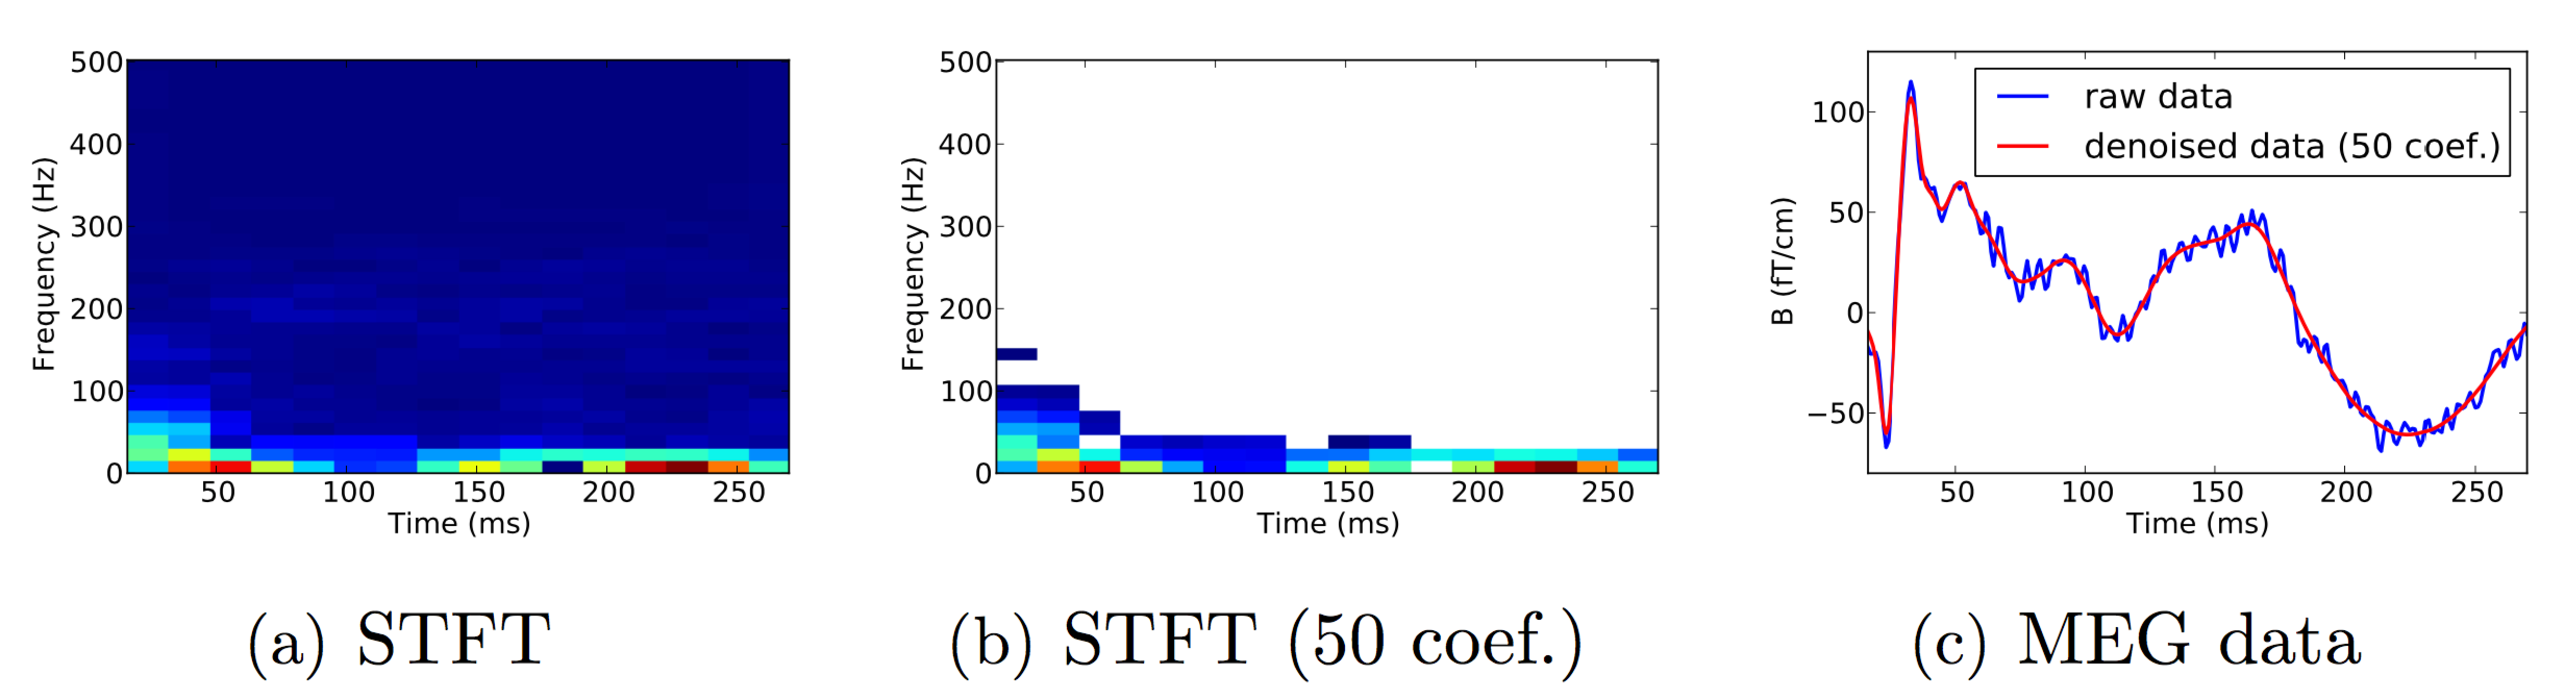
\includegraphics[width=\textwidth]{background/stft}
    \caption{a) STFT of a single channel MEG signal sampled at 1000Hz showing the sparse nature of the transformation (window size 64 time points and time shift $k_0=16$ samples). b) STFT restricted to the 50 largest coefficients. c) Original data and reconstructed data using only the 50 largest coefficients.}
	\label{fig:stft}
\end{figure}

In practice, the Gabor coefficients are computed using the Fast Fourier Transform (FFT) and not by a multiplication by a $\mathbf{\Phi}$ matrix as suggested above. Such operations can be efficiently implemented as in the LTFAT toolbox\footnote{http://ltfat.sourceforge.net} \cite{sondergaard2012linear}. Another practical concern to keep in mind is the trade-off between the size of the window $\mathbf{g}$ and the time shift $k_0$. A long window will have a good frequency resolution and a limited time resolution. The time precision can be improved with a small time shift, leading however to a larger computational cost, both in time and memory. Finally as any computation done with an FFT, the STFT implementations assume circular boundary conditions for the signal. To take this into account and avoid edge artifacts, the signal has to be windowed.\\

For more details about Gabor dictionaries, please refer to \cite{daubechies1992ten}.

\subsection{Conclusion}

This last part briefly introduced some important properties of time-frequency representations. It presented MDCT and Gabor dictionaries. It mainly explained the advantage of using the tight Gabor frames concept. The STFT or Gabor frames are time invariant, contrary to MDCT. Chapter~\ref{chapter:multiscale} will model the inverse problem in the \ac{TF} domain, which is based on the construction of Gabor frames. 

%-----------------Optimization--------------------------------------------------------------
\section{Optimization}
Due to the fact that the MEG/EEG sensors are linear combinations of the electromagnetic fields produced by all current sources, the linear forward operator, called \textit{gain matrix}, or the \textit{mixing matrix}, predicts the MEG/EEG measurements. Here we introduce the linear regression on which the formulation of the MEG/EEG inverse problem is based in this thesis.

\subsection{Linear model and regression}
%\textbf{XXX: intro to convexity...}
In statistics, linear regression consists of modeling the linear relationship between an observation $\textbf{y}$ and some explanatory variables $\mathbf{A}=[A_1,\dots ,A_n]^\top$. This relationship involves the vector of coefficients $\mathbf{x}\in\RR^m$ such that:
\begin{equation} \label{eq_linreg}
	y = Ax	
\end{equation}
% \langle\mathbf{s}, \mathbf{x}\rangle = y \enspace .
This linear model is verified for a set of observations coming from the same event, \textit{i.e.} the linear combination defined by $\mathbf{x}$ is the same for all (variable, observation) couples originating from the same event: $(\mathbf{A}_i, y_i)\in\RR^m\times\RR$ with $i\in [1,\dots ,n]$. We can note $[y_1, \dots ,y_n]^\top=\mathbf{y}\in\RR^n$ and $[\mathbf{A}_1,\dots ,\mathbf{A}_n]\in\RR^{m\times n}$. If all couples $\{(\mathbf{A}_i,y_i)\}_{i\in [1,\dots ,n]}$ verify exactly a linear model, then there exists a vector $\mathbf{x}\in\RR^m$ such that $\mathbf{Ax}=\textbf{y}$.

In a MEG/EEG application, the equivalent of $\mathbf{A}$ is the forward operator $\mathbf{G}$ which describes the linear relationship between the MEG/EEG measurements $\mathbf{M}\in\RR^{N\times T}$ ($N$ number of sensors, $T$ number of time instants) and the source activation $\mathbf{X}\in\RR^{S\times T}$ ($S$ is the number of source locations). The linear model then reads: $\mathbf{M} = \mathbf{GX}$ where $\mathbf{G}\in\RR^{N\times S}$ is the gain or the lead-field matrix (forward operator), a known instantaneous mixing matrix, which links source and sensor signals. 

In practice, the linear model is never exactly verified due to external noise. The aim of linear regression is to additionally assume that an unobserved random variable, \textit{i.e.} error term, is added to the linear relationship between the M/EEG measurements $\mathbf{M}$ and the source activation $\mathbf{X}$. The regression model can then be written similarly to Equation~\eqref{eq:meeg_ip}:
\begin{equation} \label{eq_linmeeg}
	\mathbf{M} = \mathbf{GX} + \mathbf{E}
\end{equation}
with $\mathbf{E}$ is the measurement noise, which is assumed to be additive, white, and Gaussian, \mbox{$\mathbf{E}_{.,j}\sim\mathcal{N}(0,\mathbf{I})$} for all $j$. This assumption is acceptable on the basis of a proper spatial whitening of the data using an estimate of the noise covariance \cite{engemann2015automated}.

Several methods exist to approximate the solution of the regression model. The most widely used is the \ac{OLS} approach \cite{legendre1805nouvelles}, which minimizes the sum of the squares of the errors or residuals as follows:
\begin{equation} \label{eq_ls}
	\mathbf{X^\star} \in \argmin_{\mathbf{X}\in \RR^{S\times T}}\frac{1}{2} \|\mathbf{M}-\mathbf{GX}\|_{Fro}^2
\end{equation}
There exist other types of approaches like the \ac{LAD}, also known as least absolute errors. Instead of minimizing the squares of the errors, \ac{LAD} tries to minimize the sum of the absolute values of the errors/residuals. Its advantage over \ac{OLS} is that it is more robust to outliers in the data. However the LAD is not stable, \textit{i.e.}, a small modification of the observation $\mathbf{M}$ may result in a huge variation of the estimation of $\mathbf{X}$. Moreover it can have multiple solutions, because unlike \ac{OLS}, it does not have an analytical expression but needs to be computed iteratively. This explains why the OLS approach has been the standard one, along with the fact that it has a closed-form solution.

\subsection{Regularization}

Regularization in general can be applied for different reasons. We have seen why the least squares is the standard approach in linear regression. However this approach has some drawbacks: \textit{overfitting} \footnote{Overfitting: when the model fits the training data too well and has bad generalization} and the fact that the closed-form solution is computed using $\mathbf{G}^\top\mathbf{G}$, which might not be invertible, giving rise to infinitely many solutions. This requires to set regularization.\\

In general, the penalization term will be marked $\mathcal{P}(\mathbf{X})$ as in Equation~\eqref{eq_reg} and it can take any dense or sparse form:
\begin{equation} \label{eq_reg}
	\mathbf{X}^\star = \argmin_{X\in\RR^{S\times T}}\frac{1}{2}\|\mathbf{M}-\mathbf{GX}\|_{Fro}^2 + \lambda\mathcal{P}(\mathbf{X})
\end{equation}
In the rest of this section, we list the different regularization terms $\mathcal{P}(\mathbf{X})$ as those using: dense norms, convex sparse norms, non-convex sparse norms, and structured norms.

\subsubsection*{Non-sparsity promoting norms}
Thikonov regularization \cite{tikhonov1977solutions} is the most commonly used penalty, also known as rigde regression \cite{hoerl1970ridge}. It is part of dense norms as the estimated $\mathbf{X}^\star$ is dense, even if most of its values are almost zero. It reads:
\begin{equation} \label{eq_thikonov}
	\mathbf{X}^\star = \argmin_{X\in\RR^{S\times T}}\frac{1}{2}\|\mathbf{M}-\mathbf{GX}\|_{Fro}^2 + \lambda\|\mathbf{X}\|_2^2
\end{equation}

The first term of the minimization is called the data fit, and the second term penalizes the solution by keeping the values of $\mathbf{X}$ small. We always keep the same data fit term $\frac{1}{2}\|\mathbf{M}-\mathbf{GX}\|_{Fro}^2$ and change the second penalization term depending on our priori knowledge. The penalization is controlled by the $\lambda$ parameter. The higher it is, the more penalized the regression is. An explicit solution of Equation~\eqref{eq_thikonov} is given by $\mathbf{X}^\star = (\mathbf{G}^\top\mathbf{G}+\lambda\mathbf{I})^{-1}\mathbf{G}^\top\mathbf{M}$. 

In this thesis, we are interested in sparsity promoting regularizations, which are natural for the MEG/EEG inverse problem. Indeed, it is reasonable to assume that only a few focal regions in the brain are active during a certain cognitive task.

\subsubsection*{Sparse norms: \textit{Convex norms}}
Let $\mathbf{y}\in\RR^n$ a vector. The support of $y$ is defined by the set $\mathcal{S}(y) = \{i=[1,\dots ,n] \mathrm{\ s.t.\ } \\ y[i]\neq 0\}$.
A vector is sparse if its support is small, \textit{i.e.} the cardinal $\# \mathcal{S}(y)$ is small compared to $n$.
The cardinal of $\mathcal{S}(y)$ corresponds to the $\ell_0$ pseudo-norm. The optimization problem implies then to identify $\mathcal{S}(y)$.\\

Coming back to our application, we assume that the signals $\mathbf{M}$ obtained with MEG/EEG are linear combinations of a small number of sources in the brain. This implies that only few sources in $\mathbf{X}$ are active, \textit{i.e.}, $\mathbf{X}$ is sparse. However the minimization of Equation~\eqref{eq_reg} with the $\ell_0$-norm ($\mathcal{P}(\mathbf{X})=\|\mathbf{X}\|_0$) is unfortunately an NP-hard combinatorial problem.
% This problem is difficult as we need to select the the number of sources. Furthermore, the $\ell_0$-norm is not convex \cite{natarajan1995sparse}.

Due to the above undesired properties, we need to consider a convex relaxation of the $\ell_0$-norm. The use of the least squares with the $\ell_1$-norm (i.e. $\mathcal{P}(\mathbf{X})=\|\mathbf{X}\|_1$ in Equation~\eqref{eq_reg}) is the natural approximation, since it is the closest convex norm to the $\ell_0$-norm. The $\ell_1$-norm is known as \textit{\ac{lasso}} in statistics \cite{tibshirani1996regression}, and as Basis Pursuit Denoising~\cite{chen2001atomic} in signal processing literature.

\adjustwidth{1em}{0pt}
\subsubsection*{\ac{lasso}}
\begin{equation} \label{eq_lasso}
	\mathbf{X}^\star = \argmin_{\mathbf{X}\in\RR^{S\times T}}\frac{1}{2}\|\mathbf{M}-\mathbf{GX}\|_{Fro}^2 + \lambda\|\mathbf{X}\|_1
\end{equation}
\endadjustwidth
The use of a convex approximation of the $\ell_0$-norm is convenient, as the method always converges to a globally optimal solution. There exist also very efficient algorithms.

\subsubsection*{Sparser norms: \textit{Non-Convex norms}}
These convex approaches allow for fast algorithms with guaranteed global convergence. However, the resulting source estimates are biased in amplitude and often suboptimal in terms of support recovery~\cite{candes2008enhancing}. This is particularly due to the high spatial correlation of the MEG/EEG forward model. As shown, \textbf{e.g.} in the compressed sensing literature, promoting sparsity by applying non-convex penalties, such as logarithmic or $\ell_p$-quasinorm penalties with $0 < p < 1$, can improve support identification, as well as reduce amplitude bias~\cite{candes2008enhancing,chartrand2007exact,saab2008stable}. Figure~\ref{fig:norms} shows the geometric interpretation of different norms in the 1-dimensional space. The smaller $p$, the closer is this approximation to the exact definition of sparsity. 

\begin{figure}
\centering
	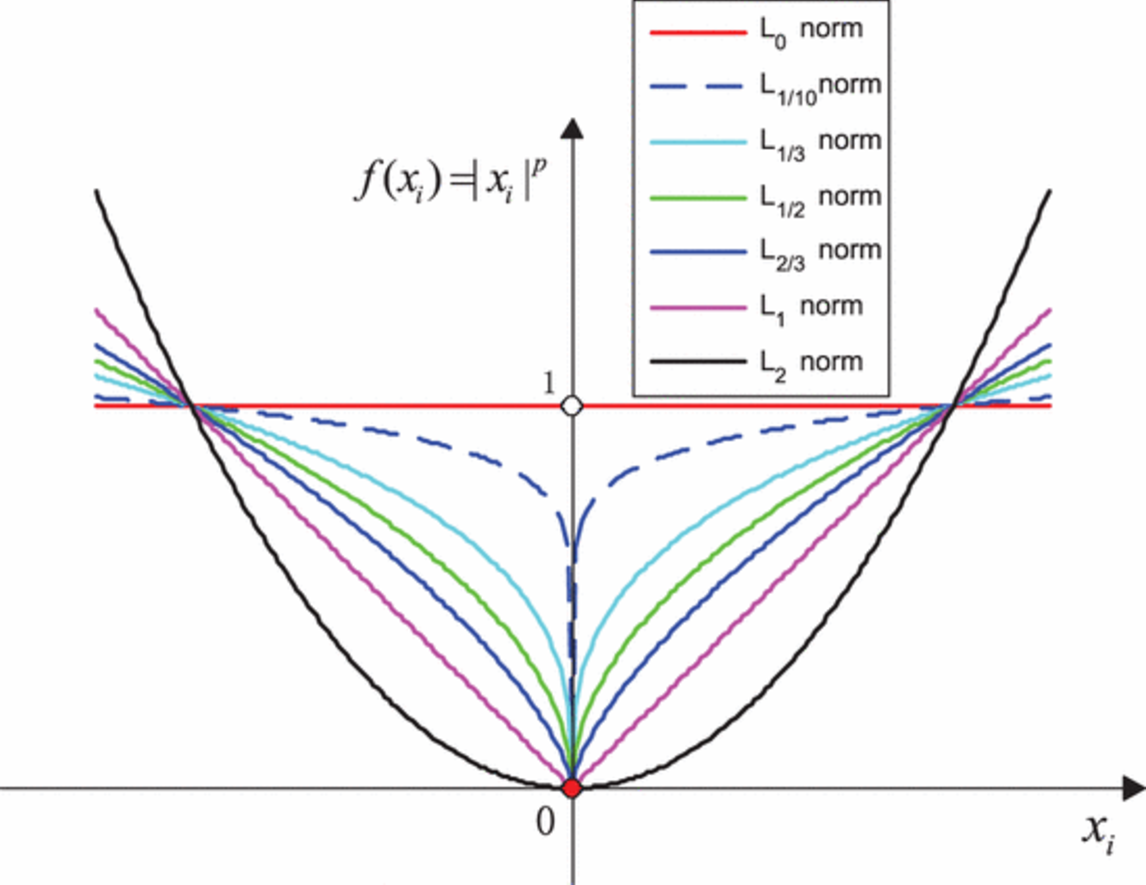
\includegraphics[width=0.7\textwidth]{background/norms}
	%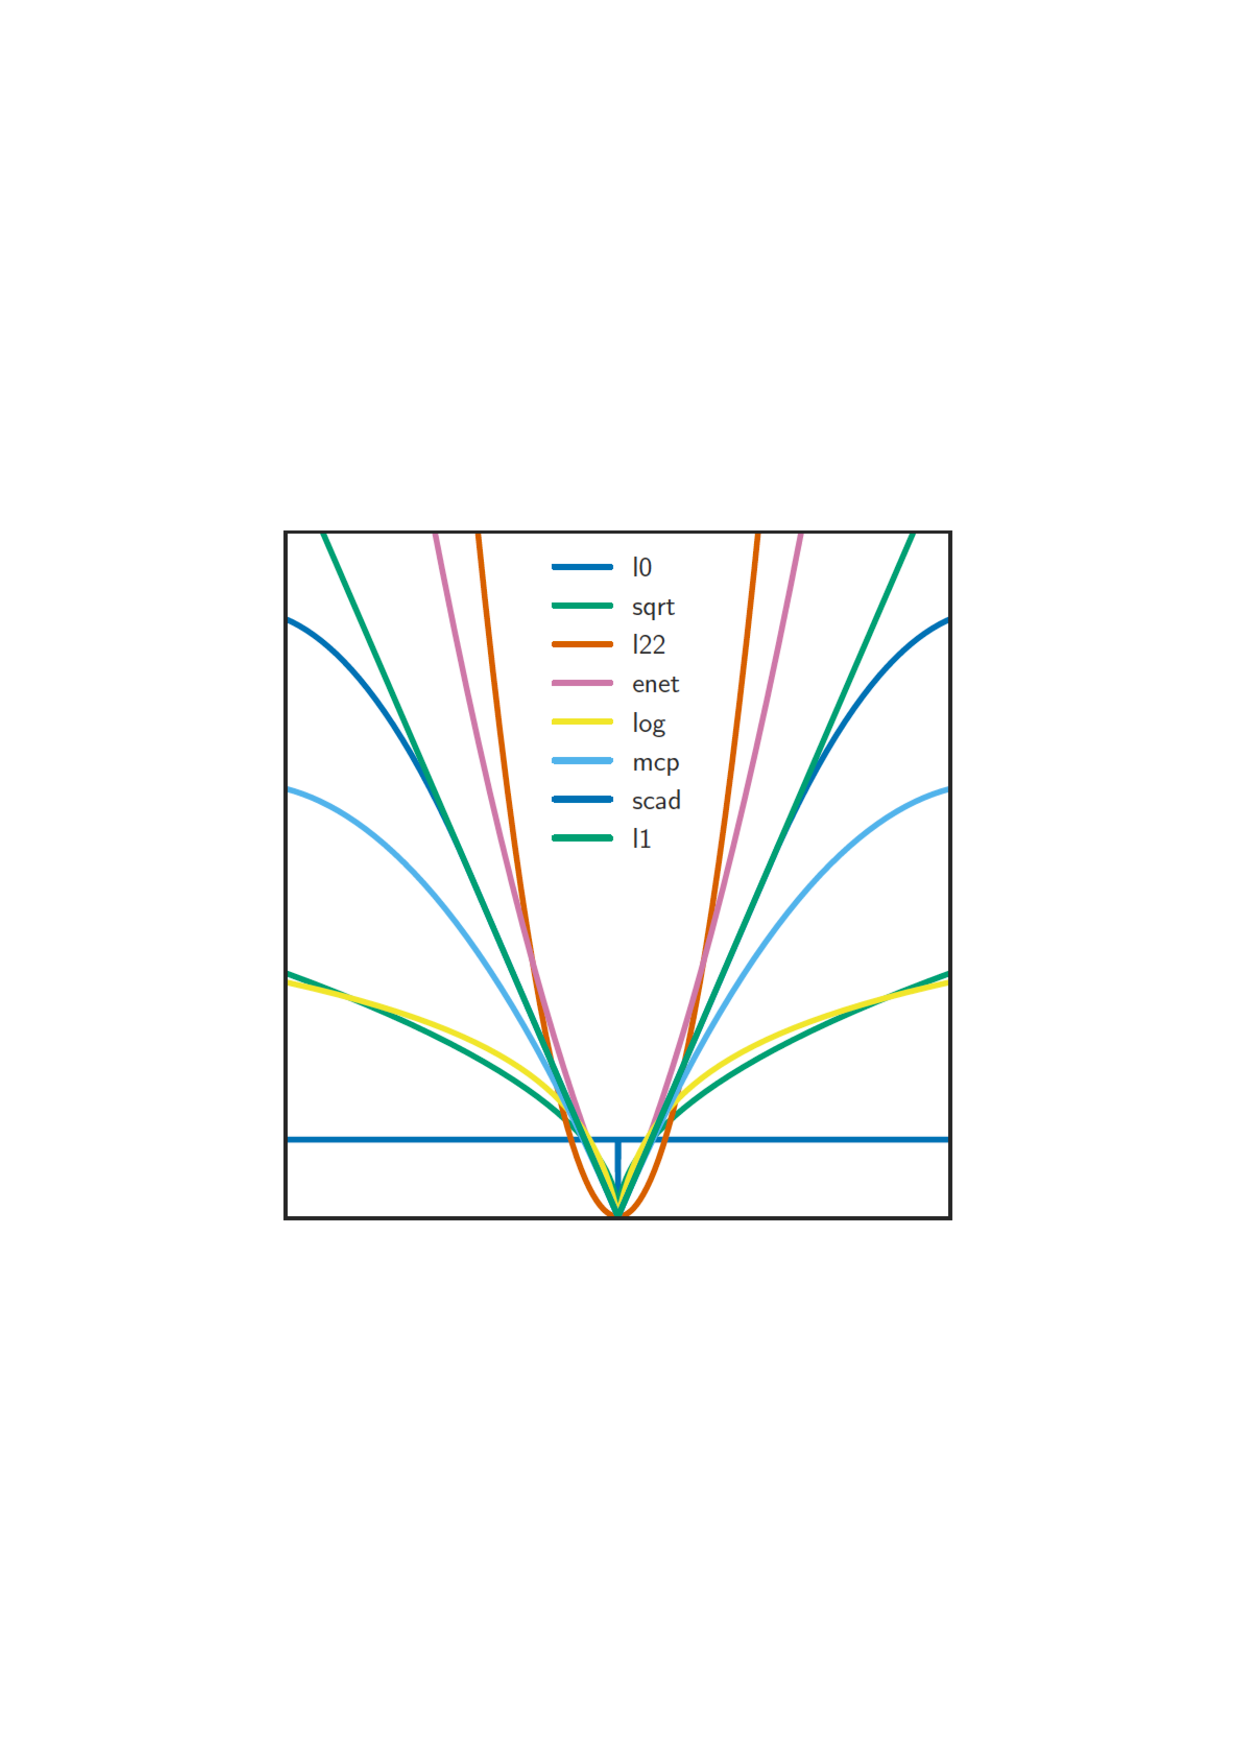
\includegraphics[trim={1cm 8cm 2cm 8cm},width=0.6\textwidth]{background/norms_methods}
    \caption{Geometric interpretation of the different norms in 1D space.}
	\label{fig:norms}
\end{figure}

We investigated the $\ell_{0.5}$-quasinorm as part of the regularization, written as:
\adjustwidth{1em}{0pt}
\subsubsection*{$\ell_{0.5}-quasinorm$}
\begin{equation} \label{eq_quasinorm}
	\mathbf{X}^\star = \argmin_{\mathbf{X}\in\RR^{S\times T}}\frac{1}{2}\|\mathbf{M}-\mathbf{GX}\|_{Fro}^2 + \lambda\|\mathbf{X}\|_{0.5}
\end{equation}
\endadjustwidth

As the $\ell_{0.5}$-quasinorm is non-convex, it cannot be solved in the same way and with the same guarantees as the $\ell_1$-norm. One algorithm for solving Equation~\eqref{eq_reg} using the $\ell_{0.5}$ quasi-norm consists in applying an iterative reweighted approach, where each iteration boils down to a convex problem with a weighted $\ell_1$ regularization.
\adjustwidth{1em}{0pt}

\subsubsection*{Weighted \ac{lasso}}
\begin{equation} \label{eq_wlasso}
	\mathbf{X}^\star = \argmin_{\mathbf{X}\in\RR^{S\times T}}\frac{1}{2}\|\mathbf{M}-\mathbf{GX}\|_{Fro}^2 + \lambda\|\mathbf{X}\|_{\mathbf{W};1}
\end{equation}
with
\begin{equation*}
	\|\mathbf{X}\|_{\mathbf{W};1}=\sum_i\sum_j W[i,j]|X[i,j]|
\end{equation*}
where $\mathbf{W}$ is the weight applied to matrix $\mathbf{X}$ aiming to regularize more the low coefficients, resulting in a higher sparsity. The update of the weight $\mathbf{W}$ will be presented in Chapter \ref{chapter:multiscale}.
\endadjustwidth

\subsubsection*{Structured Norms: \textit{non stationary sources in TF domain}}\label{sec:mixed_norms}
In some applications, like for MEG/EEG, one is not only interested in sparsity, as a-priori knowledge is available on the structure of the support of $\mathbf{X}$. To go beyond the sparsity with the $\ell_p$-norms where $0<p<1$, \cite{yuan2006model} introduced the Group \ac{lasso} in order to take grouped structures  in the data into account. It uses a mixed $\ell_2$ and $\ell_1$-norm on $\mathbf{X}$. The idea is to keep a small number of groups active ($\ell_1$) but once a group is active, then the coefficients of that group will be all nonzero ($\ell_2$).
\adjustwidth{1em}{0pt}
\vspace{-10pt}
\subsubsection*{Group \ac{lasso}}
\vspace{-10pt}
\begin{equation} \label{eq_glasso}
	\mathbf{X}^\star = \argmin_{\mathbf{X}\in\RR^{S\times T}}\frac{1}{2}\|\mathbf{M}-\mathbf{GX}\|_{Fro}^2 + \lambda\|\mathbf{X}\|_{2,1}
\end{equation}
where
\begin{equation*}	\|\mathbf{X}\|_{2,1}=\sum_i\left(\sum_j|X[i,j]|^2\right)^{1/2}
\end{equation*}
\endadjustwidth
While the Group \ac{lasso} gives only a sparse set of groups, sometimes we would like to obtain sparsity in groups and within each group. In our application, a group is basically a source, \textit{i.e.} a position in the brain. The Group \ac{lasso} is definitely convenient to obtain sparse source estimates, however it is not efficient for sources which are active only during small time windows. Toward this end, one can use Sparse Group \ac{lasso}~\cite{simon2013sparse}, which is a convex combination of the \ac{lasso} and the Group \ac{lasso} penalties.
\adjustwidth{1em}{0pt}

\subsubsection*{Sparse Group \ac{lasso}}
\begin{equation} \label{eq_sglasso}
	\mathbf{X}^\star = \argmin_{\mathbf{X}\in\RR^{S\times T}}\frac{1}{2}\|\mathbf{M}-\mathbf{GX}\|_{Fro}^2 + \lambda_1\|\mathbf{X}\|_{2,1} + \lambda_2\|\mathbf{X}\|_1
\end{equation}
If $\lambda_1=0$ then it would be equivalent to the \ac{lasso} penalty, and if $\lambda_2=0$, it results in the Group \ac{lasso} penalty.
\endadjustwidth

%----------Methods for solving sparse inverse problems-------------------------------------
\subsection{Methods for solving sparse inverse problems}
The previous section describes the MEG/EEG inverse problem as a penalized regression model. This section enumerates some methods for solving this inverse problem using sparse priors. The corresponding MEG/EEG inverse solver for the $\ell_1$-norm is the MCE solver (Minimum Current Estimate) introduced by Matsuura and Okabe \cite{matsuura1995selective}. One possible way to solve the $\ell_1$ penalty is to use the Iterative Least Squares (IRLS). IRLS consists in iteratively computing weighted LS by setting appropriate weights. This is based on the fact that a weighted $\ell_2$-norm: $\|\mathbf{x}\|_{\mathbf{w};2}=\sum_i w[i]^k |x[i]|^2$ is equal to the $\ell_1$-norm: $\|x\|_1=\sum_i|x[i]|$, when $w[i]^k=1/|x[i]|$, where $k$ denotes the iteration index. This corresponds to WMN in Section~\ref{section_distributed}. Similar iterative weighted methods are used to solve the (Sparse) Group \ac{lasso} corresponding to mixed-norms in both standard and time-frequency domains presented in Section~\ref{section_distributed}. Other methods based on the proximity operator are used to solve non-differentiable convex optimization problems. The idea is to alternate the minimization over the smooth convex data fit using a small gradient step and the computation of the proximal operator associated with the penalty which is non-smooth.\\

Indeed, the MEG/EEG inverse problem can be written as:
\begin{equation}
\hat{\mathbf{X}} = \argmin_{\mathbf{X}\in\RR^{SO\times T}}f(\mathbf{X}) = \argmin_{\mathbf{X}\in\RR^{SO\times T}}(g(\mathbf{X}) + \lambda\mathcal{P}(\mathbf{X})) \mathrm{\;with\;} \lambda>0 \enspace .
\end{equation}
Here $g(\mathbf{X}):\CC^{SO\times T}\rightarrow\RR$ is a convex differentiable function with Lipschitz-continuous gradient. The regularization function $\mathcal{P}(\mathbf{X}):\CC^{SO\times T}\rightarrow\RR$ is a non-smooth function, typically a combination of norms or quasi-norms, inducing sparsity in the time or time-frequency domain.

\subsubsection*{Proximal operators}
Let $\mathit{h}:\RR^n\rightarrow\RR$ be a convex, non differentiable function. The proximity operator associated with $\mathit{h}$ and $\lambda\in\RR_+$ denoted by
$\prox_{\lambda\mathit{h}}:\RR^n\rightarrow\RR^n$ is given by:

\begin{equation}
\prox_{\lambda\mathit{h}}(\mathbf{y})=\argmin_{\mathbf{x}\in\RR^n}\frac{1}{2}\|\mathbf{y}-\mathbf{x}\|_2^2+\lambda\mathit{h}(\mathbf{x})
\end{equation}

This corresponds to the inverse problem where $\mathbf{G}=\mathbf{I}$. To be able to solve the problem with non-smooth penalties and $\mathbf{G}\neq\mathbf{I}$, one needs to introduce the iterative \textit{forward-backward} algorithm \cite{moreau1965proximite}. Each iteration computes the proximity operator of the penalty as:
\begin{equation}
\mathbf{X}^{(k+1)}[:,j]=\prox_{\mu\lambda\mathcal{P}}(\mathbf{X}^{(k)}[:,j]+\mu\mathbf{G}^\top(\mathbf{M}[:,j]-\mathbf{GX}^{(k)}[:,j]), \forall j\in [1,\dots ,T]
\end{equation}
$\mu$ stands for the step size and has been proved to satisfy $0<\mu<\|\mathbf{G}^\top\mathbf{G}\|_2^{-1}$. In practice, it is fixed to $\mu=\frac{1}{\mathcal{L}}=
 \|\mathbf{G}^\top\mathbf{G}\|_2^{-1}$, where $\mathcal{L}$ denotes the Lipschitz constant. $k$ represents the iteration index. For more details refer to~\cite{moreau1965proximite,combettes2005signal,daubechies2004iterative}.

If the penalty is set to be the $\ell_{2,1}$-norm as in Equation~\eqref{eq_glasso}, the solution is obtained by row-wise soft thresholding. These proximal gradient methods are known as the forward-backward algorithm, thresholded Landweber iterations, or the \ac{ISTA} or \ac{FISTA}~\cite{bach-etal:2012,parikh2014proximal}. FISTA or any proximal gradient method can be applied when the objective function is a sum of two terms, a convex smooth term and non-smooth term for which the proximity operator is available.
% It consists of a forward or gradient step based on $g(\mathbf{X})$ with step size $\mu$, and a backward step based on a proximity operator of $\mathcal{P}(\mathbf{X})$.
A detailed algorithm of FISTA applied to Group \ac{lasso} can be found in Algorithm~\ref{alg:FISTA}. 

{\fontsize{4}{4}\selectfont
\begin{algorithm}[t]
\SetKwInOut{Input}{Input}
\SetKwInOut{Init}{init}
\SetKwInOut{Parameter}{Auxiliary variables}
\caption{\textsc{Group \ac{lasso} with FISTA}}
\Input{$\bfM, \bfG $, $\lambda > 0$}
\Parameter{$\mathbf{Y}$, $\mathbf{X}_0\in\RR^{S\times T}$, $\tau_0\in\RR$}

1. Initialization: $\mathbf{X}\in\RR^{S\times T}$, $\mathbf{Y}=\mathbf{X}$, $\tau=1$, and $0 < \mu < \mathcal{L}^{-1} = \|\mathbf{G}^\top\mathbf{G}\|^{-1}$\\
2. \textbf{repeat}\\
3. \hspace{4pt} $\mathbf{X}_0 = \mathbf{X}$\\
4. \hspace{4pt} $\tau_0 = \tau$\\
5. \hspace{4pt} $\mathbf{X} = \prox_{\mu\lambda\|.\|_{2,1}}(\mathbf{Y}-\mu\nabla g(\mathbf{X}))$ with $\nabla g(\mathbf{X})= -\mathbf{G}^\top(\mathbf{M}-\mathbf{GX})$ \\
6. \hspace{4pt} $\tau = \frac{1+\sqrt{1+4\tau^2_0}}{2}$\\
7. \hspace{4pt} $\mathbf{Y} = \mathbf{X} + \frac{\tau_0 - 1}{\tau}(\mathbf{X}-\mathbf{X}_0)$\\
8. \textbf{until} convergence\\
\Return{$\mathbf{X}$}\\
\label{alg:FISTA}
\end{algorithm}
}

However, as seen before, the $\ell_1$-norm is not very appropriate for M/EEG applications as it does not take the temporal correlation of the data into account. For the spatio-temporal solvers such as TF-MxNE or irTF-MxNE presented in Chapter~\ref{chapter:multiscale}, one needs to introduce the proximity operator for these composite penalties.

\adjustwidth{1em}{0pt}
\subsubsection*{Proximity operator of $\ell_{2,1}+\ell_1$}
Let $\mathbf{Y}\in\RR^{S\times T}$; $\mathbf{X}=\prox_{\lambda_1\|\cdot\|_1+\lambda_2\|\cdot\|_{2,1}}(\mathbf{Y})\in\RR^{S\times T}$ is given for each coordinate $(s,t)$ by:

\begin{equation} \label{prox_mixed}
	X[s,t]=\frac{Y[s,t]}{|Y[s,t]|}(|Y[s,t]|-\lambda_1)_+\left(1-\frac{\lambda_2}{\sqrt{\sum_t(|Y[s,t]|-\lambda_1)_+^{2}}}\right)_+
\end{equation}
where for $z\in\RR, (z)_+ =\max(0,z)$ and by convention $\frac{0}{0}=0$.
\endadjustwidth


%\subsubsection*{Coordinate Gradient Descent}
%Gradient descent is a first-order iterative optimization algorithm for finding the minimum of a function. To find a local minimum of a function using gradient descent, one takes steps proportional to the negative of the gradient (or of the approximate gradient) of the function at the current point.


\subsubsection*{Block Coordinate Descent: BCD} \label{section:BCD}
Other methods for solving the MEG/EEG inverse problem with non-smooth penalties exist. We mention here the block coordinate descent (BCD) scheme \cite{tseng2010approximation}. BCD is an extension of the well known coordinate descent (CD)~\cite{li-osher:2009,nesterov2012efficiency}. CD is based on the idea of decomposing a large optimization problem into a sequence of one-dimensional optimization problems. \\

BCD was used to solve the Group \ac{lasso} in~\cite{rakotomamonjy2011surveying,qin2013efficient}, it is based on the same idea of alternating between a gradient step and the computation of the proximity operator of $\mathcal{P}(\mathbf{X})$ (for instance: $\ell_{2,1}+\ell_1$). BCD is used on block-separable schemes where a block is a set of coordinates and can be defined depending on the data. Here a block maps a location in the brain, \textit{i.e.}, a block is one source. Similarly to the CD method, the order in which the different blocks are processed can be cyclic, random which improves theoretical performance~\cite{tseng2001convergence,wei2012doa}. \\

As both BCD and FISTA are based on the same idea of alternating between the gradient and the proximal operator, their difference is that BCD uses at each step a subproblem specific to one block. The subproblem per block has a closed form solution, which involves applying the group soft-thresholding operator, the proximity operator associated to the $\mathcal{P}(\mathbf{X})$, for instance that defined in Equation~\ref{prox_mixed} when using $\ell_{2,1}+\ell_1$ ($\mathcal{P}(\mathbf{X}) = \|\mathbf{X}\|_{2,1}+\|\mathbf{X}\|_1$. Accordingly, the closed form solution for the BCD subproblems solving the Group \ac{lasso} problem can be derived as:
\begin{equation*} \label{eq_bcd_glasso}
\bar{\mathbf{X}}_s^{(k)} = \mathbf{X}_s^{(k-1)}+\mathbf{\mu}_s\mathbf{G}^\top_s(\mathbf{M} - \mathbf{GX}^{(k-1)})
\end{equation*}
\begin{equation}
\tilde{\mathbf{X}}_s^{(k)} = \tilde{\mathbf{X}}_s^{(k)}\max(1-\frac{\mathbf{\mu[s]\lambda}}{\max(\|\bar{\mathbf{X}}_s^{(k)}\|_{Fro}, \mathbf{\mu}[s]\lambda)}, 0)
\end{equation}
The step length $\mathbf{\mu}[s]$ for each BCD subproblem is determined by $\mathbf{\mu}[s]=\mathcal{L}_s^{-1}$ with $\mathcal{L}_s=\|\mathbf{G}_s^\top\mathbf{G}_s\|$ being the Lipschitz constant of the data-fit restricted to the $s^{th}$ source location. This step length is typically larger than the step length applicable in any proximal gradient method, which is upper-bounded by the inverse of $\mathcal{L} = \|\mathbf{G}^\top\mathbf{G}\|$.

\subsubsection*{Optimality conditions and stopping criterion}\label{section:duality_gap}

\textbf{Stopping criterion:} The standard way is to check if the solution at iteration $k$ has not been improved more than a fixed tolerance threshold $\epsilon$, for either the objective function $|f(\mathbf{X}^{(k-1)})-f(\mathbf{X}^{(k)})|<\epsilon$, or the source estimate itself $\|\mathbf{X}^{(k-1)}-\mathbf{X}^{(k)}\|_{\infty}<\epsilon$. This is an acceptable strategy, although not the best one. A more rigorous criteria would be based on the \textit{duality gap} \cite{boyd2004convex,bach2012optimization}.\\

\textbf{Duality gap:} It is a way to check the optimality criterion when optimizing a cost function $f$. For a subset of convex problems, the Slater's conditions apply, therefore the gap at the optimum is exactly zero~\cite{Boyd_Vandenberghe04}. Computing the gap needs to derive first a dual formulation of the original problem, also called the \textit{primal} problem. For a general minimization problem, the minimum of the primal objective function $f_p(\mathbf{X})$ is bounded below by the maximum of the dual objective function $f_d(\mathbf{X})$. Then, the duality gap is defined as the difference between the minimum of the primal cost function $f_p$ and the maximum of the dual cost $f_d$. For a value of of $\mathbf{X}^{(k)}$ of the primal variable at iteration $k$, if one can exhibit a dual variable $\mathbf{Y}^{(k)}$, the duality gap $\eta{(k)}$ is defined as:

\begin{equation}
\eta^{(k)}=f_p(\mathbf{X}^{(k)})-f_d(\mathbf{Y}^{(k)}) \geq 0
\end{equation}

At the optimum (corresponding to $\hat{\mathbf{X}}$), if the $\mathbf{Y}^{(k)}$ is well chosen, $\eta^{(k)}$ is $0$. By exhibiting a pair $(\mathbf{X}^{(k)}, \mathbf{Y}^{(k)})$, one can guarantee that $\|f_p(\mathbf{X}^{(k)}) - f_p(\hat{\mathbf{X}})\| \leq \|f_p(\mathbf{X}^{(k)})-f_d(\mathbf{Y}^{(k)})\|$. A good stopping criterion is therefore given by a duality gap $\eta^{(k)}<\epsilon$. The solution meeting this condition is called $\epsilon$-optimal. The challenge in practice is to find an expression for $f_d$ and to be able to associate a good $\mathbf{Y}$ with a given $\mathbf{X}$. Experimental studies showed that for whitened data a duality gap lower than $10^{-6}$ does not produce distinguishable solutions~\cite{Gramfort_Kowalski_Hamalainen12}. For more details on how to compute the duality gap in this kind of problems, see~\cite{bach2012optimization,Gramfort_Kowalski_Hamalainen12,strohmeier-etal:16}\\

%Moreover, the Karush-Kuhn-Tucker (KKT) conditions of the Fenchel-Rockafellar duality theorem give a natural mapping from the primal space to the dual space:
%\begin{equation}
%\mathbf{Y}^{(k)}=\mathbf{M}-\mathbf{GX}^{(k)}
%\end{equation}

\subsubsection*{Screening rules and active set} \label{section:active_set}
The regularization term $\mathcal{P}(\mathbf{X})$ used in this thesis promotes spatial sparsity, which makes most of the blocks of $\hat{\mathbf{X}}$ equal to zero. We can thus reduce the computation time by primarily updating blocks that are likely to be non-zero, while keeping the remaining blocks at zero. For this purpose, data-dependent sweep patterns (such as greedy approaches based on steepest descent~\cite{li-osher:2009,wei2012doa}) or active set strategies can be applied~\cite{friedman-etal:2010,roth-etal:08}.\\

The active set strategy can be used for both Group \ac{lasso} and Sparse Group \ac{lasso} based on~\cite{roth2008group,wang2014two}. The main idea is to start with $\mathbf{X}=0$, which corresponds to an empty active set $\Gamma=\{\}$. We estimate an initial active set of sources $\Gamma$ by evaluating the Karush-Kuhn-Tucker (KKT) optimality conditions~\cite{roth2008group,wang2014two}, which states that $\hat{\mathbf{X}}_s=0$ under some conditions depending on the regularization term. We select the $N$ sources that violates the KKT conditions the most (\textit{e.g.} $N=10$). Subsequently, we restrict the source space to the sources in $\Gamma$ and estimate $\hat{\mathbf{X}}^{\Gamma}$ with convergence controlled by the duality gap. After convergence of this restricted optimization problem, we check whether $\hat{\mathbf{X}}^{\Gamma}$ is an $\epsilon$-optimal solution for the original problem (without restricting the source space to $\Gamma$). If $\hat{\mathbf{X}}^{\Gamma}$ is not an $\epsilon$-optimal solution indicated by $\eta \leq \epsilon$, we re-evaluate the KKT optimality conditions and update the active set $\Gamma$ by adding the $N$ sources that violate again these optimality conditions. The same procedure is then repeated with warm start.


\subsubsection*{Comparison of the different solvers}\label{section:comparison_solvers}
In Strohmeier et al.~\cite{strohmeier-etal:16}, the BCD scheme was used for solving the MEG/EEG inverse problem. For the problem at hand, BCD outperforms FISTA proposed in a former work in~\cite{gramfort2012mixed}. BCD converges faster due to the reasons discussed in the BCD subsection~\ref{section:BCD}. Taking bigger step depending on the current block makes the algorithm go faster to the optimal solution.

\begin{figure}
	\centering
	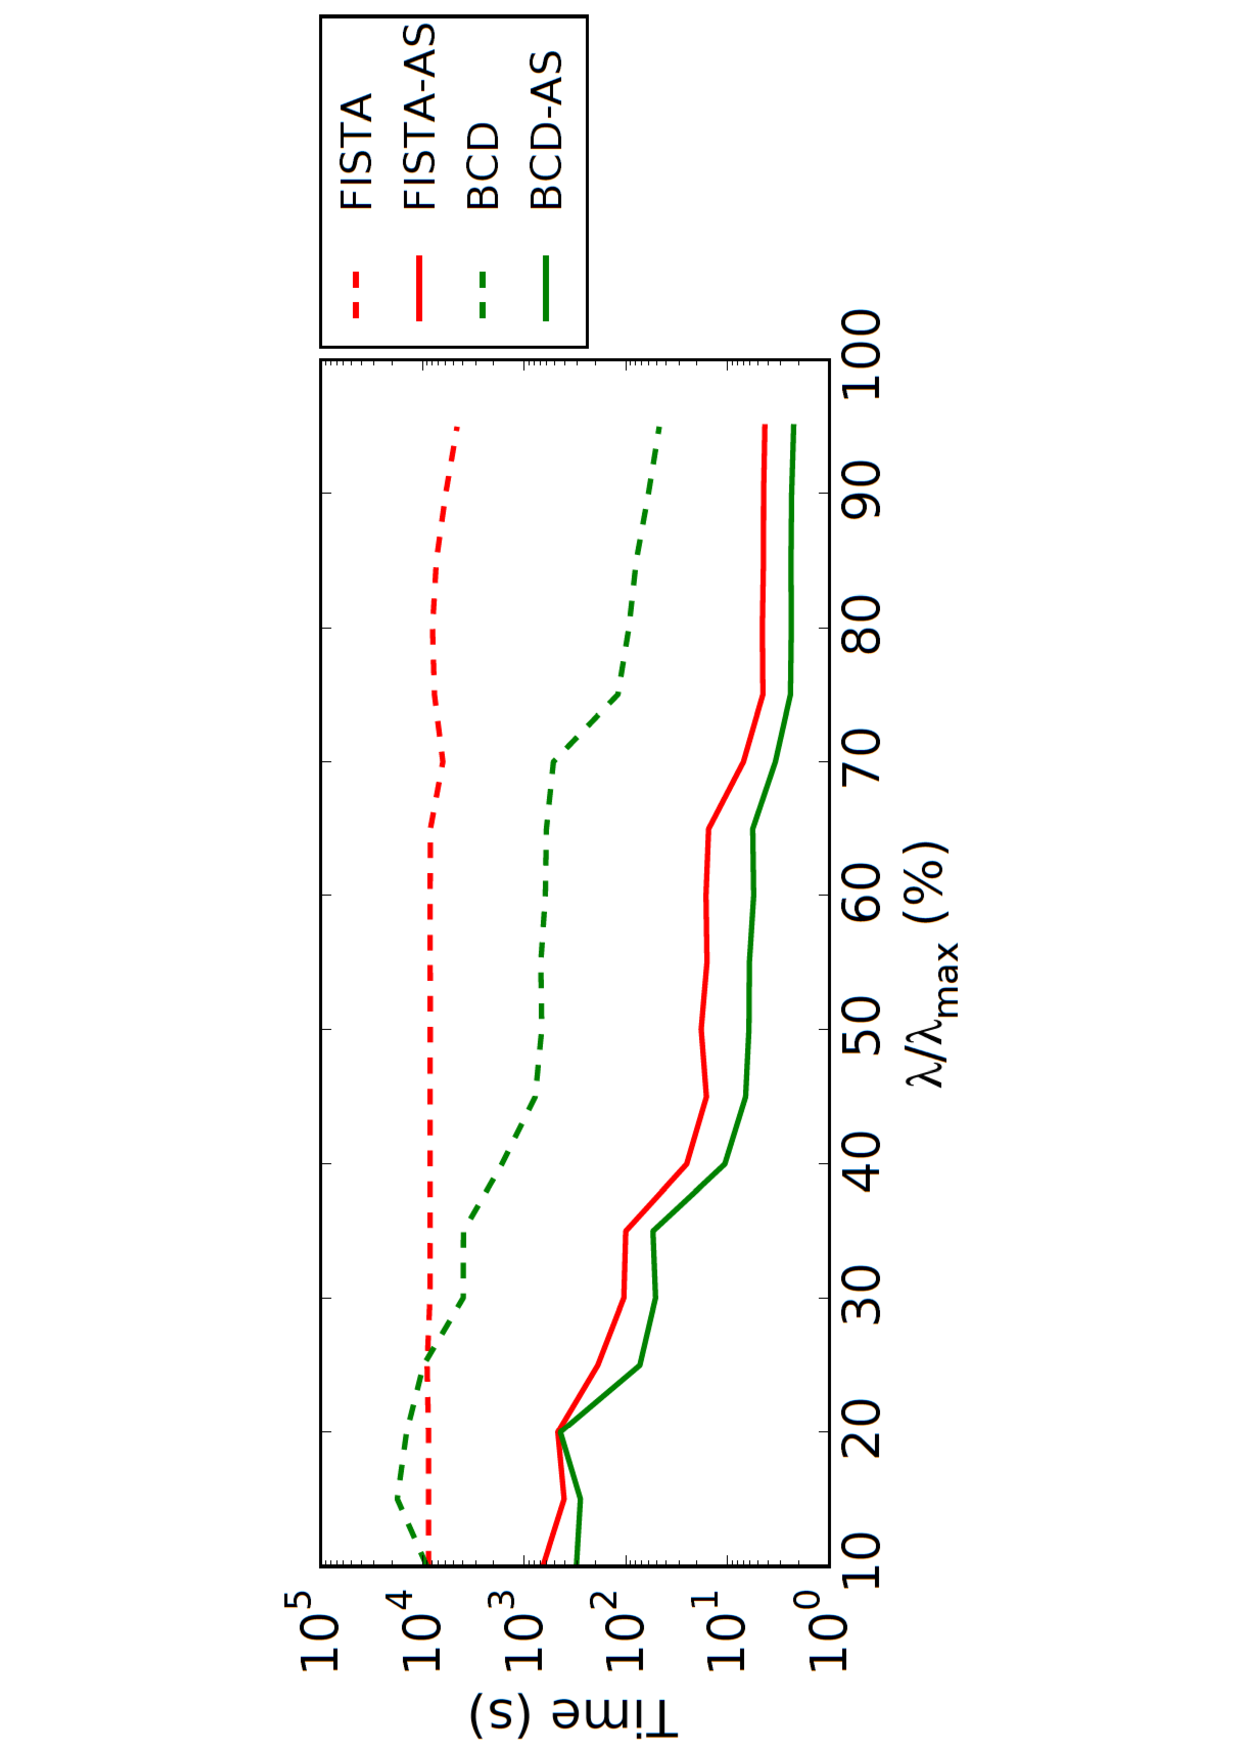
\includegraphics[trim={1cm 0.5cm 2cm 0.5cm},angle=270,width=0.95\textwidth]{background/comparison_fista_bcd}
    \caption{Computation time as a function of $\lambda$ for group \ac{lasso} on real MEG data using BCD and FISTA with (solid) and without (dashed) active set strategy. The size of the data was: 306 sensors, 7498 cortical locations, and free orientation (O=3)}
    \label{fig:comparison_fista_bcd}
\end{figure}
%\textbf{XXX: need to say what is $\lambda_{max}$ somewhere in this chapter}
Combining the BCD and the active set strategy reduces the computation time by a factor of 100 and allows us to compute the group \ac{lasso} on real MEG/EEG data in a few seconds. All the experimental results shown in the rest of this thesis will be obtained by using BCD with active set strategy.

\subsection{Conclusion}
This chapter gives all the needed background which has been used to develop and demonstrate the upcoming results. It demonstrated how to model the inverse problem as a regularized regression problem. It defined the multiple priors that have been used in the literature including the sparse approaches that are of interest in this thesis. Then it introduced some of the methods for solving the different convex optimization problems. This is again not an exhaustive list and not all details have been presented here. 

This chapter also defined the state of the art of the MEG/EEG inverse problem and how research in this field have been evolving. From the penalized regression formulation to the hierarchical Bayesian formulation, I will show in the next chapters how this thesis tries to bridge the gap between those two communities. Especially, the aim is to take advantage of each part, the computationally fast solvers developed so far by one community and the ability to quantify uncertainties of the solution in the second community.
% Chapter 2

\chapter{Source localization with multi-scale dictionaries} % Main chapter title

\label{chapter:multiscale} % For referencing the chapter elsewhere, use \ref{Chapter1} 
\noindent\makebox[\linewidth]{\rule{0.75\paperwidth}{0.4pt}}
\noindent\makebox[\linewidth]{\rule{0.75\paperwidth}{0.4pt}}

\localtableofcontents % local toc

\noindent\makebox[\linewidth]{\rule{0.75\paperwidth}{0.4pt}}
\noindent\makebox[\linewidth]{\rule{0.75\paperwidth}{0.4pt}}
\newpage

%----------------------------------------------------------------------------------------
\section{Introduction}
In chapter~\ref{chapter:background}, we have seen all the background of the inverse problem in the MEG and EEG field. We justified the motivation for having sparse priors as regularization for the regression problem. Sparse priors were presented under different approaches. This chapter considers the variational problem in the Time-Frequency domain by fixing the penalization term as a sparse group LASSO as in Equation~\eqref{eq_sglasso}, with $\lambda_1$ a hyperparmeter over space, and $\lambda_2$, a second hyperparameter over time. Figure~\ref{fig:set_norms} justifies this choice. It shows how $\ell_{21}+\ell_1$ allows for modeling non-stationary sources which cannot be estimated with $\ell_2$ or $\ell_{21}$ due to the non-convexity promoting $\ell_2$-norm, while the $\ell_1$ estimate is completely scattered and unstructured.\\

\begin{figure}
\centering
	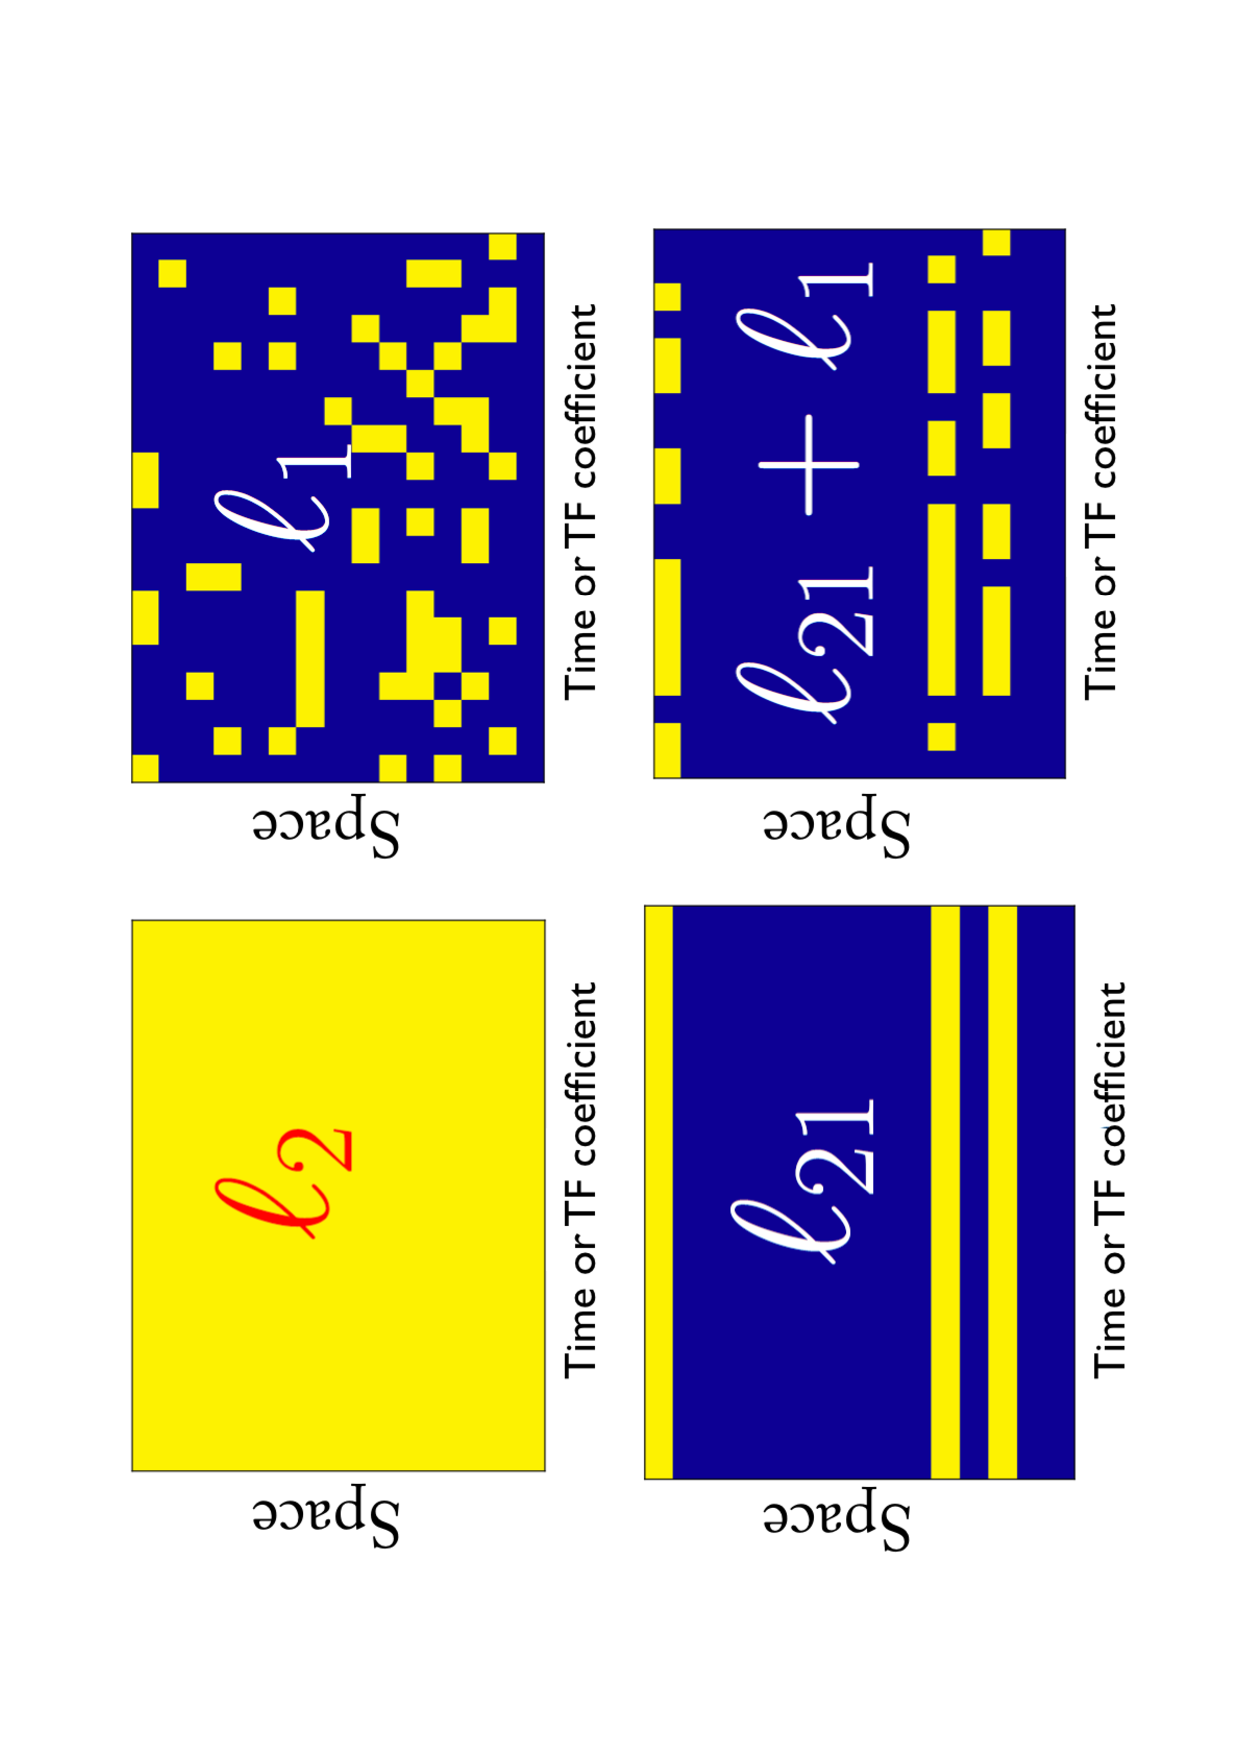
\includegraphics[angle=270,width=0.9\textwidth]{multidict/set_norms}
    \caption{Sparsity patterns promoted by the different regularizations: $\ell_2$ all non-zero, $\ell_1$ scattered and unstructured non-zero, $\ell_{21}$ block row structure, and $\ell_{21} + \ell_1$ (TF domain) block row structure with intra-row sparsity. Yellow color indicates non-zero coefficients.}
    \label{fig:set_norms}
\end{figure}

This chapter describes the source localization in the Time-Frequency (TF) domain. We have showed why localizing the source in the TF domain was a "true" spatio-temporal approach taking the time correlation into account.
The Time-Frequency Mixed Norm Estimate (TF-MxNE) \cite{Alex13}, Spatio-Temporal Unifying Tomography (STOUT) \cite{castano2015solving} and the iterative reweighted TF-MxNE (irTF-MxNE) \cite{daniel15} improve reconstruction of transient and non-stationary sources by promoting structured sparsity in the TF domain. Those methods compute a sparse group lasso on the TF coefficients. TF-MxNE and STOUT apply a composite convex penalty, the sum of an $\ell_{2, 1}$-mixed-norm and an $\ell_{1}$-norm penalty, on the Gabor transform of the source time courses. On the other hand, irTF-MxNE applies a composite \emph{non-convex} penalty, the sum of an $\ell_{2, 0.5}$-quasinorm and an $\ell_{0.5}$-quasinorm penalty on the TF coefficients.
The non-convex penalties have been shown to outperform convex approaches both in terms of source recovery and amplitude bias \cite{candes2008enhancing,daubechies2010iteratively} as explained in Chapter~\ref{chapter:background}. However, the choice of an optimal Gabor dictionary for decomposing the data remains difficult.\\

This issue of the choice of the dictionary is specially encountered when a mixture of signals is available in the data, \textit{e.g.}, short transient signal right after the onset of a stimuli, and slower brain waves afterward. A choice of a unique dictionary describing both signals in a sparse way is hard. We show in this chapter how to incorporate a multi-scale dictionary in the iterative reweighted optimization algorithm, \textit{i.e.} multiple dictionaries with different scales concatenated to fit short transients and slow waves at the same time, while keeping computational efficiency. The optimization problem is solved in the same way as irTF-MxNE \cite{daniel15}, \textit{i.e.}, each iteration is a weighted TF-MxNE, which we solve using block coordinate descent (BCD) and an active set strategy \cite{friedman2010regularization}. %We compare irTF-MxNE with and without a multi-scale dictionary on simulated and real MEG data. %As both solvers are able to recover the active set size,
We demonstrate the benefit of the multi-scale dictionary in terms of reconstructed source time courses and temporal unmixing of activations.

\section{Inverse problem in the Time-Frequency domain} \label{irtfmxne}

Using a dictionary of TF atoms, such as a tight Gabor frame, $\mathbf{\Phi} \in \mathbb{C}^{T \times C}$ ($T$ samples, $C$ atoms), the neuronal activation $\mathbf{X} \in \mathbb{R}^{SO \times T}$ ($S$ sources, $O$ orientation) can be modeled as a linear combination of atoms, $\mathbf{X}=\mathbf{Z\Phi}^{\mathcal{H}}$, where $\mathbf{Z} \in \CC^{SO \times C}$ is the TF coefficients matrix. A Gabor frame $\mathbf{\Phi}$ is tight (section~\ref{section:TF}) when the Euclidean norm of the input signal and the vector of TF coefficients are proportional ($\|\mathbf{Z}\|_2^2 = A_\mathbf{\Phi} \|\mathbf{X}\|_2^2$ where $A_\mathbf{\Phi}>0$). When $A_\mathbf{\Phi}=1$ the frame is said to be normalized. We will use tight frames in the following.

The MEG/EEG measurements $\mathbf{M} \in \mathbb{R}^{N \times T}$ ($N$ sensors) follows the forward model:
\begin{equation} \label{eq:reg_prob_tf}
    \mathbf{M} = \mathbf{GX} + \mathbf{E} = \mathbf{GZ \Phi}^{\mathcal{H}} + \mathbf{E}
\end{equation}

where $\mathbf{G} \in \mathbb{R}^{N \times SO}$ stands for the forward operator. $\mathbf{E} \in \mathbb{R}^{N \times T}$ is the measurement noise, which can be assumed to be additive white noise: $\mathbf{E}[:, j] \sim \mathcal{N}(0, \mathbf{I})$ for all $j$ after spatial whitening \cite{denis}. Estimating the coefficients $\mathbf{Z}$ given the measurement $\mathbf{M}$ is an ill-posed problem and constraints have to be imposed on $\mathbf{Z}$ to obtain a unique source estimate, as described for $\mathbf{X}$ in the last chapter. For analyzing evoked responses, we assume that the neuronal activation is spatially sparse and temporally smooth. This corresponds to a row sparsity~\cite{Alex13}, which we promote by applying a composite non-convex regularization $\mathcal{P}(\mathbf{Z})$ (See Figure~\ref{fig:set_norms}). The associated regularized regression problem is:
\begin{equation} \label{eq:penalized_reg_tf}
    \mathbf{Z}^\star = \argmin_{\mathbf{Z}} \frac{1}{2}\|\mathbf{M - GZ\Phi^\mathcal{H}}\|^2_{Fro} + \mathcal{P}(\mathbf{Z})
\end{equation}
with
\begin{equation}
%\begin{split}
%	\mathcal{P}(\mathbf{Z}) & = \lambda_{space}\mathcal{P}_{1}(\mathbf{Z}) + \lambda_{time}\mathcal{P}_{2}(\mathbf{Z}) \\
%& = \lambda_{space}\|\mathbf{Z}\|_{2,0.5} + \lambda_{time}\|\mathbf{Z}\|_{0.5} \\
%\end{split}
	\mathcal{P}(\mathbf{Z}) = \lambda_{space}\|\mathbf{Z}\|_{2,0.5} + \lambda_{time}\|\mathbf{Z}\|_{0.5}
\end{equation}
where $\lambda_{space} > 0$, $\lambda_{time}>0$. A large regularization parameter $\lambda_{space}$ will lead to a spatially very sparse solution or even an empty solution, while a large $\lambda_{time}$ will promote sources with smooth time series and might loose sharp aspect of the neural activity.

\section{Fast iterative reweighted TF-MxNE with tight frames}
Given a dictionary $\mathbf{\Phi}$, the optimization problem in Equation~\eqref{eq:penalized_reg_tf} can be solved by iteratively minimizing convex surrogate problems~\cite{daniel15}. The regularization term at each iteration $k$ is a weighted convex mixed norm that can be written as:
\begin{equation} \label{eq:weights_optim}
%   \mathcal{P}(\mathbf{Z}) = \lambda_{space}\sum_{s}\sqrt{\|\mathbf{Z}[s,:]\|_2} + \lambda_{time}\sum_{s,c}\sqrt{|\mathbf{Z}[s,c]|}
    \mathcal{P}(\mathbf{Z}) = \lambda_{space}\|\mathbf{Z}\|_{\mathbf{W}_1^{(k)};2,1} + \lambda_{time}\|\mathbf{Z}\|_{\mathbf{W}_2^{(k)};1}
\end{equation}
with $\forall s,c$,
\begin{equation*}
\begin{aligned}
    \mathbf{W}_1^{(k)}[s,c] &= \left(2\sqrt{\|\hat{\mathbf{Z}}^{(k-1)}[s,:]\|_2 + \epsilon^{(k-1)}}\right)^{-2} \\
    \mathbf{W}_2^{(k)}[s,c] &= \left(2\sqrt{|\hat{\mathbf{Z}}^{(k-1)}[s,c]| + \epsilon^{(k-1)}}\right)^{-1}
\end{aligned} \enspace ,
\end{equation*}
%
where $\mathbf{W}_1$ and $\mathbf{W}_2$ are the weights applied to the TF coefficients, and $\mathbf{\hat{Z}}^{(k-1)}$ are the estimated coefficients at iteration $(k-1)$. $\epsilon^{(k-1)} \in \mathbb{R}^+$ is used to prevent infinite weights. To have an intuition about the update rule for the weights, one can prove that updating the weights with $w_i$=$|x_i|^{p-2}$ leads to a solution of the $\ell_p$-norm penalized problem.\\
%Here, $\epsilon$ is set to $0$ and infinite weights are handled as in \cite{daniel15}.

For solving Equation~\eqref{eq:penalized_reg_tf}, we use BCD~\cite{tseng2010approximation}. The algorithm boils down to sequentially computing a gradient step and the proximity operator of the $\ell_{2,1}+\ell_1$ norm for each block $s$ of coefficients (See Section~\ref{section:BCD}). Here a block maps to a location in the brain. One update of a block of coefficients is given by first a gradient step:
\begin{align} \label{eq:block_update}
    \mathbf{R} &= \mathbf{M} - \mathbf{G}\hat{\mathbf{X}} \\
    \bar{\mathbf{X}}[s,:] &= \hat{\mathbf{X}}[s,:] + \mathbf{\mu}[s]\mathbf{G}[:,s]^\top\mathbf{R} \\
    \bar{\mathbf{Z}}[s,:] &= \bar{\mathbf{X}}[s,:]\mathbf{\Phi}
    % \mathbf{R} &= \mathbf{M} - \mathbf{G}\hat{\mathbf{Z}}\mathbf{\Phi}^{\mathcal{H}} \\
    % \bar{\mathbf{Z}}[s,:] &= \hat{\mathbf{Z}}[s,:] + \mathbf{\mu}[s]\mathbf{G}[:,s]^\mathbf{T}\mathbf{R}\mathbf{\Phi} \\
\end{align}
followed by the computation of the proximity operator of the weighted $\ell_{2,1}+\ell_1$ described in Chapter~\ref{chapter:background}-Equation~\ref{prox_mixed}:
\begin{equation} \label{prox_l1}
\begin{aligned}
    \tilde{\mathbf{Z}}[s,c] &= \bar{\mathbf{Z}}[s,c]\left(1 - \frac{\mathbf{\mu}[s]\lambda_{time}\mathbf{W}_2^{(k)}[s,c]}{|\bar{\mathbf{Z}}[s,c]|} \right)_+
\end{aligned}
\end{equation}
\begin{equation} \label{prox_l21}
\begin{aligned}
    \hat{\mathbf{Z}}[s,c] &= \tilde{\mathbf{Z}}[s,c]\left(1 - \frac{\mathbf{\mu}[s]\lambda_{space}\sqrt{\mathbf{W}_1^{(k)}[s,c]}}{\|\tilde{\mathbf{Z}}[s,:]\|_2}\right)_+
\end{aligned}
\end{equation}
When $\mathbf{\Phi}$ is a tight frame, $\mathbf{\mu}[s]$ is the step length for each BCD subproblem and it is given by $\mathbf{\mu}[s]=\sqrt{\mathbf{A}_{\mathbf{\Phi}}}(\|\mathbf{G}[:,s]^T\mathbf{G}[:,s]\|)^{-1}$. This step length, \textit{i.e.} the inverse of the Lipschitz constant restricted to the source $s$ is typically larger than the step length applicable in iterative proximal gradient methods, which is upper bounded by $\|\mathbf{G}^T\mathbf{G}\|^{-1}$. This implies a bigger step to speed up the convergence.
Finally:
\begin{equation}
    \hat{\mathbf{X}}[s,:] = \hat{\mathbf{Z}}[s,:]\mathbf{\Phi}^\mathcal{H}
\end{equation}

Equation~\eqref{prox_l1} and \eqref{prox_l21} are respectively solutions of the proximity operator for the weighted $\ell_1$-norm and for the weighted $\ell_{2,1}$-norm. As the $\ell_1$ proximity operator shrinks coefficients towards zero, if a block of coefficients were set to zero by the $\ell_{2,1}$ proximity operator, it would also be set to zero after the application of the $\ell_1$ proximity operator. As a consequence, it is possible to know just by applying the $\ell_{2,1}$ proximity operator to $\bar{\mathbf{X}}[s,:]$ if the set of coefficients $\tilde{\mathbf{Z}}[s,:]$ will be set to zero. Note that this is just a sufficient condition and we may have to compute all steps to know if the block is set to zero. This is summarized in the following lemma.

\begin{lemma}
    Let $\mathbf{\Phi}$ be a frame with constant $A_{\mathbf{\Phi}}$, if $\|\bar{\mathbf{X}}[s,:]\|_2$ $\leq \mathbf{\mu}[s]\lambda_{space}\sqrt{\mathbf{W}_1^{(k)}[s,c]} / \sqrt{A_{\mathbf{\Phi}}}$ then $\hat{\mathbf{Z}}[s,c] = 0$, $\forall c$.
\end{lemma}

Computing the TF decomposition at each iteration can be costly. The consequence of the lemma is that for a lot of source locations one can avoid computing their TF decomposition during the optimization just by computing the $\ell_{2}$-norm of the time courses after the gradient step.
To speed up the computation even more, we combine the BCD scheme~\ref{section:BCD} with an active set strategy~\ref{section:active_set}~\cite{friedman2010regularization}, which primarily updates sources that are likely to be active, while keeping the remaining sources inactive.

\subsection*{Orientation constraints}
Let $\mathbf{Z}_s\in\CC^{3\times C}$ be the block of the $\mathbf{Z}\in\CC^{3S\times C}$	corresponding to the $s^{th}$ source and $\mathbf{Z}[1,:]$ being the activity of the dipole oriented normal to the cortical surface, and $\mathbf{Z}[2,:]$ and $\mathbf{Z}[2,:]$ the two other orientation tangent to the surface. We modify the $\ell_1$-norm and the $\ell_{2,1}$-norm for the free orientation constraints as follow:
\begin{align*}
\|\mathbf{Z}\|_1 &= \sum_{s,c}\sqrt{|\mathbf{Z}_s[1,c]|^2 + \frac{1}{\kappa^2}|\mathbf{Z}_s[2,c]|^2 + \frac{1}{\kappa^2}\mathbf{Z}_s[3,c]|^2} \\
\|\mathbf{Z}\|_{2,1} &= \sum_s\sqrt{\sum_c |\mathbf{Z}_s[1,c]|^2 + \frac{1}{\kappa^2}|\mathbf{Z}_s[2,c]|^2 + \frac{1}{\kappa^2}\mathbf{Z}_s[3,c]|^2}
\end{align*}
where $s$ indexes the source location and $c$ the TF coefficient. When $\kappa=1$, no orientation contraint is applied and the modified penalties amount to grouping the orientation in a common $\ell_2$-norm.

\section{Inverse problem with multi-scale tight Gabor frames}
A tight Gabor frame is computed by setting two parameters: the length of the window (window size), and an overlap parameter (time shift). The window size defines the time/frequency resolution, if its length is short, it would be more focus on time than frequency, and vice versa, if it is long, it will be more focus on frequency than in time. The time resolution also depends on the time shift parameter. The time shift parameter defines the time step from one window to another (section~\ref{section:TF}). This affects the redundancy of the dictionary. A dense sampling of the TF space, however, increase the complexity on both time and memory.\\

Each source waveform is a sparse linear combination of atoms from this dictionary. Fixing those parameters is then critical for having an optimal dictionary. %This makes the choice of the parameters important when they are fixed and not learned.
Learning the dictionary might be a solution to avoid fixing the parameters, or the need to have an overcomplete dictionary covering a broad range of scales. However, learning both $\mathbf{Z}$ and $\mathbf{\Phi}$ simultaneously is a non-convex optimization problem, for which one needs to alternate between a convex optimization for the two variables~\cite{montoya2014regularized}. \\

%Setting the number of atoms to be learned and the stopping criterion is also challenging.

Let us define a multi-scale TF dictionary, where we concatenate $Q$ tight Gabor frames $\mathbf{\Phi}_q$, $ 1 \leq q \leq Q$, with different resolutions. One can realize that this union of tight frames $\mathbf{\Phi} = [\mathbf{\Phi}_1, \dots, \mathbf{\Phi}_Q]$ is also a tight frame with $A_\mathbf{\Phi} = \sum_q A_{\mathbf{\Phi}_q}$. The strategy presented in the previous section~\ref{irtfmxne} is therefore still relevant for a multi-scale dictionary, where the activation $\mathbf{Z}$ is a concatenation of $\mathbf{Z}_1, \mathbf{Z}_2, ..., \mathbf{Z}_Q$. Algorithm~\ref{alg:multiscale_tfmxne_activeset} describes how to solve the inverse problem in the TF domain with a multi-scale dictionary.

{\fontsize{4}{4}\selectfont
%above is to make smaller fonts in algorithm
\begin{algorithm}[t]
\SetKwInOut{Input}{input}
\SetKwInOut{Init}{init}
\SetKwInOut{Parameter}{param}
\caption{\textsc{multi-scale TF-MxNE with active set strategy}}
\Input{$\bfM, \bfG, \mathbf{\Phi}=[\mathbf{\Phi}_1, \dots, \mathbf{\Phi}_Q], \lambda_{space} > 0, \lambda_{time}$, and $\epsilon>0$}
% \Parameter{ To add }
\Init{$\mathbf{Z}\in\RR^{SO\times C}$, $\Gamma=\{\}$, $\eta=f_p(\mathbf{Z})-f_d(\mathbf{Y})$, $\mathbf{\mu}$ with $\mathbf{\mu}[s]=\mathcal{L}^{-1}_s=\|\mathbf{G}_s^\top\mathbf{G}_s\|^{-1}$}
\While{
		$\eta \geq \epsilon$
	  }
	  {
	  	$\Gamma^\star \subseteq {s \hspace{3pt} | \hspace{3pt} \|Prox_{\lambda_{time}\|.\|_1}(\mathbf{G}_s^\top(\mathbf{M}-\mathbf{GZ\Phi}\mathcal{H})\Phi)\|_{Fro} > \lambda_{space} }$
	  	
	  	$\Gamma = \Gamma \cup \Gamma^\star$
	  	
	  	$\mathbf{Z}^{\star\Gamma}\leftarrow$ Solve Algorithm~\ref{alg:multiscale_tfmxne_bcd} with $\mathbf{\mu}$, and $\Gamma$
	  	
	  	$\mathbf{Z}=\mathbf{Z}^{\star\Gamma}$ for $i\in\Gamma$, else 0

	  	$\eta=f_p(\mathbf{Z})-f_d(\mathbf{Y})$
	  }
\label{alg:multiscale_tfmxne_activeset}
\end{algorithm}
}

{\fontsize{4}{4}\selectfont
%above is to make smaller fonts in algorithm
\begin{algorithm}[t]
\SetKwInOut{Input}{input}
\SetKwInOut{Init}{init}
\SetKwInOut{Parameter}{param}
\caption{\textsc{multi-scale TF-MxNE with BCD}}
\Input{$\bfM, \bfG, \mathbf{\Phi}, \mathbf{\mu}, \lambda_{space} > 0, \lambda_{time} > 0, \epsilon > 0$, and $\Gamma^\star$ }
% \Parameter{ To add }
\Init{$\eta=f_p(\mathbf{X})-f_d(\mathbf{Y})$}
\While{
		$\eta \geq \epsilon$
	  }
	  {
	  	\For{
	  			$s\in\Gamma^\star$
	  		}
	  		{
	  			$\mathbf{Z}_s = Prox_{\mathbf{\mu}[s](\lambda_{space}\|.\|_{2,1}+\lambda_{time}\|.\|_1)}(\mathbf{Z}_s+\mathbf{\mu}[s]\mathbf{G}^\top_s(\mathbf{M}-\mathbf{GZ\Phi}^\mathcal{H})\mathbf{\Phi})$
	  		}
	  	$\eta = f_p(\mathbf{X})-f_d(\mathbf{Y})$
	  }
\label{alg:multiscale_tfmxne_bcd}
\end{algorithm}
}


\section{Experiments with different dictionaries}
%----------------------------------------------------------------------------------------
We first evaluate the accuracy of irTF-MxNE with and without multi-scale on realistic simulations. We then apply our new solver on MEG somatosensory data.

\subsection{Simulation}
We generated a realistic simulation dataset based on a fixed-orientation source model with 7549 cortical locations and 102 magnetometers. Two of these locations were selected to be active in the primary and secondary somatosensory cortex (S1 and S2). The corresponding time courses are shown in Fig. \ref{fig:simulation}-a in blue (S1) and green (S2). We have both a transient source around 40 ms and slow waves afterwards around 70, 100 and 150 ms. The irTF-MxNE solver improves the source recovery \cite{daniel15}. Therefore, we do not compare the solvers presented here over the active set size or an $F_1$ measure, %(based on the Recall and Precision)
as both solvers are already able to recover all the sources. % due to the \textit{non-convex} optimization.
We evaluate our approach by computing  %$RMSE=\|X_{sim}-X_{est}\|_{Fro}$ and
the explained variance between simulated source courses and the source estimation from each solver as follows:
\begin{equation}
	\theta = 1 - \frac{\|GX_{sim}-GX_{est}\|^2_{Fro}}{\|GX_{sim}\|^2_{Fro}} \enspace
\end{equation}

Fig.~\ref{fig:simulation}-b shows the explained variance for the irTF-MxNE with different dictionaries over a logarithmic grid of $\lambda_{space}$. The first Gabor dictionary is constructed with 64 samples (64 ms) window and 4 samples time shift (green), the second Gabor dictionary is constructed with 16 samples window and 2 samples time shift (red) and the third one is the combination of the two dictionaries (blue). We observe that the irTF-MxNE solver using the combination of two dictionaries outperforms the solver with each dictionary separately in terms of explained variance measure over all parameters range. Higher values of $\log(\lambda_{space})>1.2$ impose high penalization on the active set size, resulting in a too sparse source estimate, where the solution does not explain the measurement anymore. The results show on simulation a source reconstruction improvement, where it leads to a larger explained variance.

\begin{figure}
\centering
	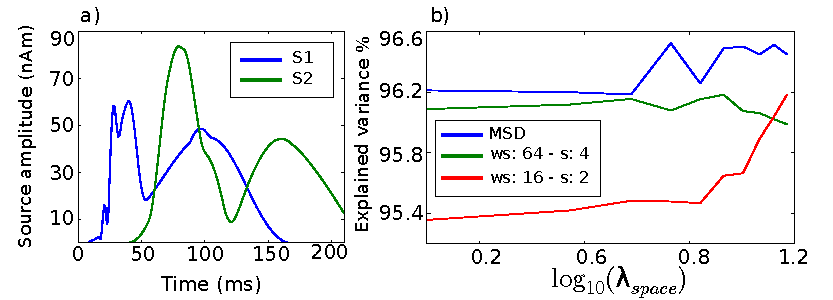
\includegraphics[width=0.85\textwidth]{multidict/fig_sim}
    \caption{(a) Simulated source time courses in S1 (blue) and S2 (green). (b) The explained variance for irTF-MxNE using two different dictionaries: long window size (ws) 64 with time shift (s) 4 (green), and small ws 16 with s 2 (red). The combination of the two dictionaries is shown in blue. This shows how the multi-scale dictionary (MSD) improves the explained variance.}
    \label{fig:simulation}
\end{figure}

\subsection{Experimental results with MEG somatosensory data}
To demonstrate the advantage of irTF-MxNE with a multi-scale dictionary over the basic irTF-MxNE, we tested different parameters for different solvers on a MEG dataset: somatosensory study of the MIND dataset (for details \cite{weisend2007paving}). The evoked is shown in Figure~\ref{fig:evoked_mind}. One can already notice this mixture of brain waves in the evoked. Sharper waves right after the onset in the evoked are due to a nice alignment of the trials which their information is not lost after averaging. This is mainly known as a response of the primary somatosensory area (S1) which answers quickly after a painless electrical stimulation of the median nerve. It is clearly seen from the evoked also this longer wave which comes later around 70ms. This is what makes this data a challenging dataset and a very good one for testing the multi-scale solver.

\begin{figure}
\centering
	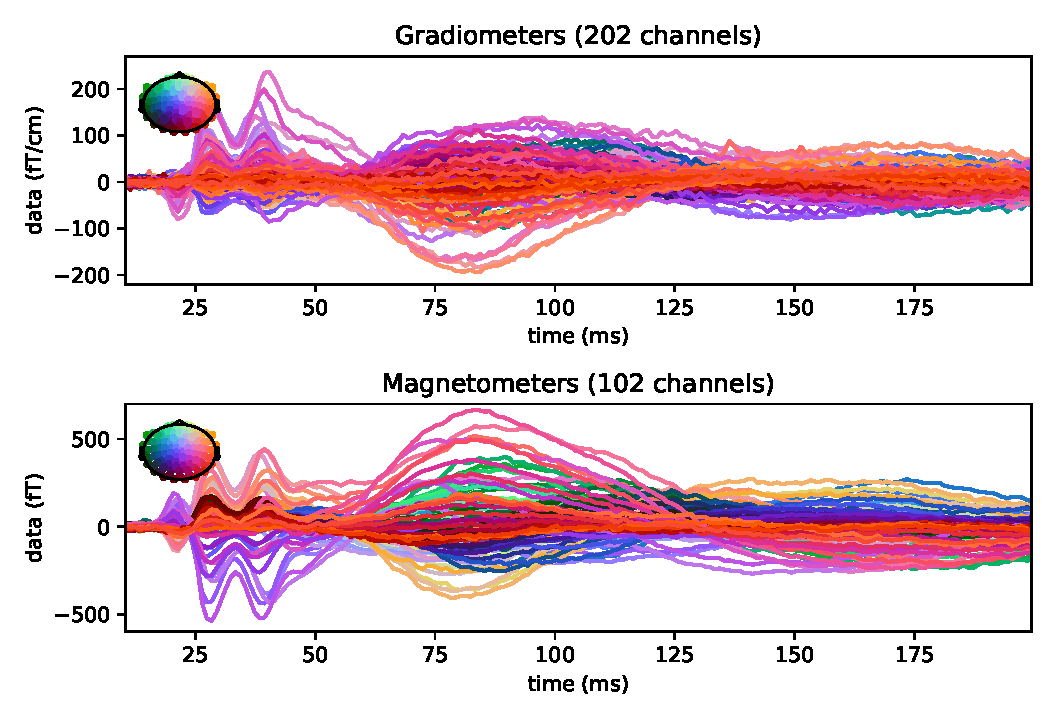
\includegraphics[width=0.9\textwidth]{multidict/evoked_mind_MEG}
    \caption{Somatosensory evoked response after preprocessing and averaging (gradiometers and magnetometers data).}
    \label{fig:evoked_mind}
\end{figure}

Source estimation was first performed using several solvers: irTF-MxNE, irMxNE~\cite{strohmeier2014iterative} and dSPM~\cite{dale2000dynamic}. Regarding irTF-MxNE, two dictionaries were tested (both STFT dictionaries). A dictionary with a 64 samples window and a 4 samples time shift, which leads to smooth source courses; and a dictionary with a 16 samples window and a 2 samples time shift, which helps capture short transient sources. After inspection of the residual in the Figure~\ref{fig:residual_mind}, results showed that at least four sources are necessary to capture all evoked components. 

We have therefore fixed the parameters of the irTF-MxNE solvers so we obtained only four sources while explaining as much variance as possible. After that, we experimented with a set of different parameters and we show two of them $\lambda_{time}=1.5$ and $\lambda_{time}=2.5$ to demonstrate their impact on the smoothness of the different time sources obtained.
The parameters were chosen in such a way to reduce the residual \textit{i.e.} to maximize the explained data by having at least four sources. 
Figure~\ref{fig:MEG_dics} (a-b) demonstrates the four time courses obtained with irTF-MxNE using the short window dictionary for the selected values of $\lambda_{time}$.

\begin{figure}
\centering
	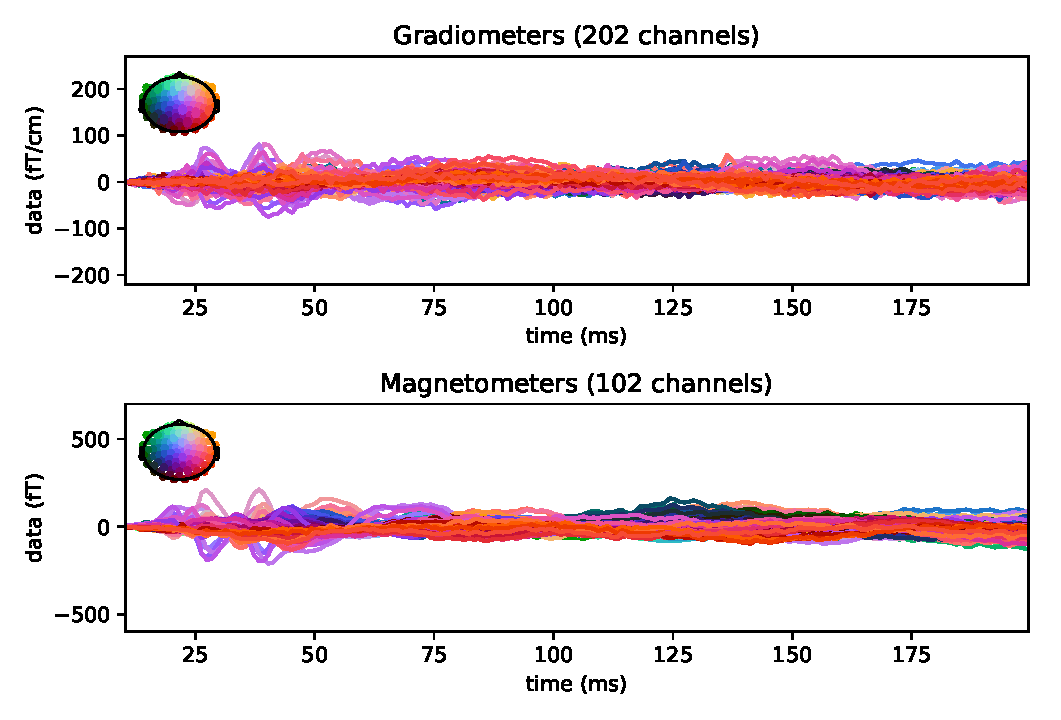
\includegraphics[width=0.9\textwidth]{multidict/residual_mind_MEG}
    \caption{Residual of the somatosensory data after applying the multi-scale irTF-MxNE.}
    \label{fig:residual_mind}
\end{figure}

We show that for high values of $\lambda_{time}$ (b), the solver is not able to capture the short transient component around 30 ms. While for a small value (a), the unmixing is not reliable since the light blue and the green source estimates catch the activity from the red source. Additionally, the time courses are not smooth. On the other hand, Figure~\ref{fig:MEG_dics} (c-d) demonstrate the four time courses obtained with irTF-MxNE using the long window dictionary for the selected $\lambda_{time}$. The figure confirms that both parameters are not able to capture the transient effect after the stimulus, although the time courses are smooth. These four sub-figures reveal that one need a short window to capture the transient effect of the brain signal (See Figure~\ref{fig:residual_long_dic}), while it needs to have a long window to capture the long waves and to have smooth source estimates. This result demonstrates how a combination of the two dictionaries is critical to acquire source estimates with high precision, but the hyperparameters needs to be tuned as well as shown in this Figure~\ref{fig:MEG_dics} that their values change drastically the results.

\begin{figure}
\centering
	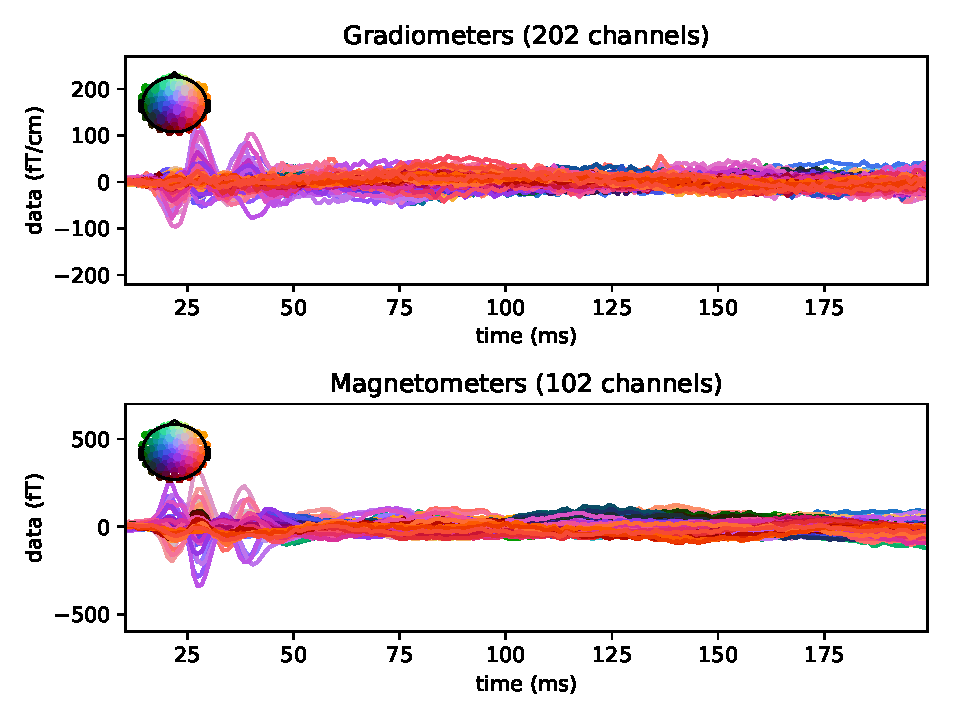
\includegraphics[width=0.9\textwidth]{multidict/residual_mind_MEG_long_dictionary}
    \caption{Residual of the somatosensory data after applying irTF-MxNE with a long window dictionary (window size = 64, time shift = 4). The transient part of the brain signal is left in the residual as it cannot be modeled by the long dictionary.}
    \label{fig:residual_long_dic}
\end{figure}

Moreover, Figure~\ref{fig:MEG_dics} (e) displays the amplitudes obtained with MxNE for five sources, as for MxNE, one is not able to obtain the four relevant sources unmixed (See for more demonstrative figures~\cite{gramfort2012mixed}). We notice that the light blue source in Figure~\ref{fig:MEG_dics} (a) to (d) appears as two separate sources in (e): light blue and purple. If we increase the $\lambda$ parameter, we increase the amplitude bias due to the $l_1$ norm of the solver. If we set it too high ($\lambda=50$) we obtain four sources, but the blue source which is relevant to the study would be removed and the duplicated purple source is kept. The last panel Figure~\ref{fig:MEG_dics} (f) displays the source estimates for dSPM values corresponding to the four locations of the sources obtained with the irTF-MxNE. These sub-figures show that none of MxNE or dSPM solvers are able to obtain smooth sources without any leakage between the time courses.

\begin{figure}
\centering
	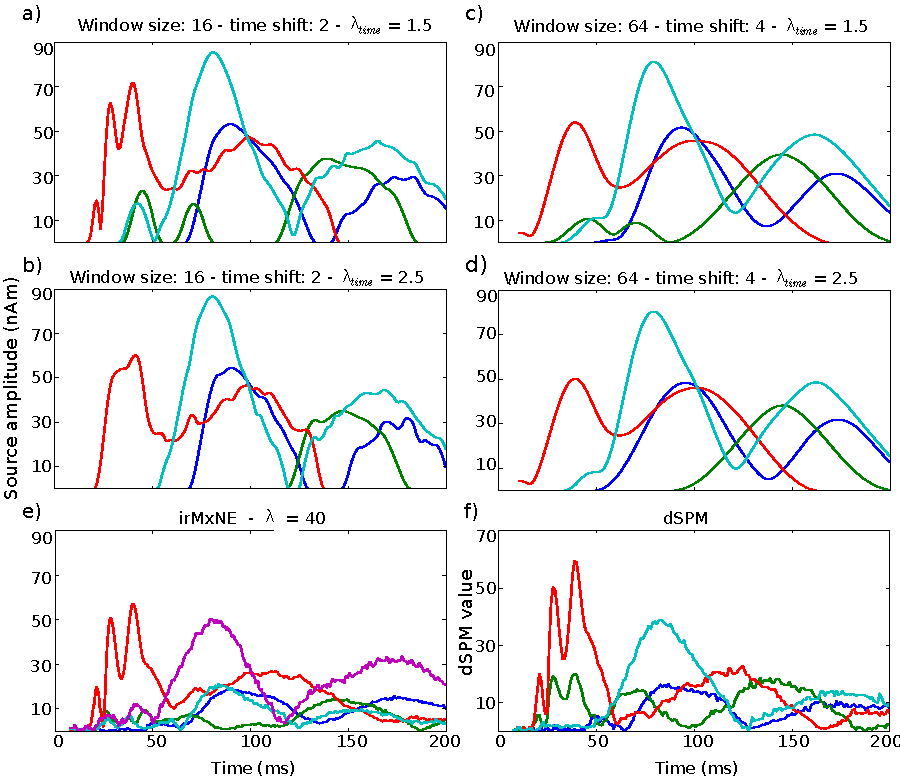
\includegraphics[width=0.95\textwidth]{multidict/fig_dics}
    \caption{Source reconstruction using somatosensory data with different solvers. (a) - (b) irTF-MxNE on a small window dictionary with $\lambda_{time}=1.5$ and $\lambda_{time}=2.5$ respectively. (c) - (d) irTF-MxNE on a long window dictionary with $\lambda_{time}=1.5$ and $\lambda_{time}=2.5$ respectively. From (a) to (d) $\lambda_{space}=28.5$ (e) MxNE for $\lambda=40$ and (f) dSPM activation for the four activated sources.}
    \label{fig:MEG_dics}
\end{figure}

Source estimation was then achieved using irTF-MxNE with the combination of the two dictionaries.
Figure~\ref{fig:MEG} shows source reconstruction using the multi-scale irTF-MxNE for the regularization parameters $\lambda_{space}=28.5$ and $\lambda_{time}=1.5$. Each source's location is marked by a sphere in Figure~\ref{fig:MEG} left, and its amplitude over time is color-coded in the right panel. The results show a suitable succession of the sources. The transient source (red) is the only source explaining the event related field until 48 ms. This red source corresponds to the contralateral primary somatosensory cortex (cS1) located in the postcentral gyrus of the parietal lobe (right hemisphere (rh)). The red sphere on the lateral view coincides with the smeared dSPM activation around 40 ms. The second source (light blue) corresponds to the secondary somatosensory cortex (cS2), and also occurs with dSPM activation around 80 ms. About 100 ms after stimulus, additional cortical sources are activated, such as ipsilateral secondary somatosensory cortex (iS2) (blue-lh), and contralateral medial wall (green-rh). 

\begin{figure}
\centering
	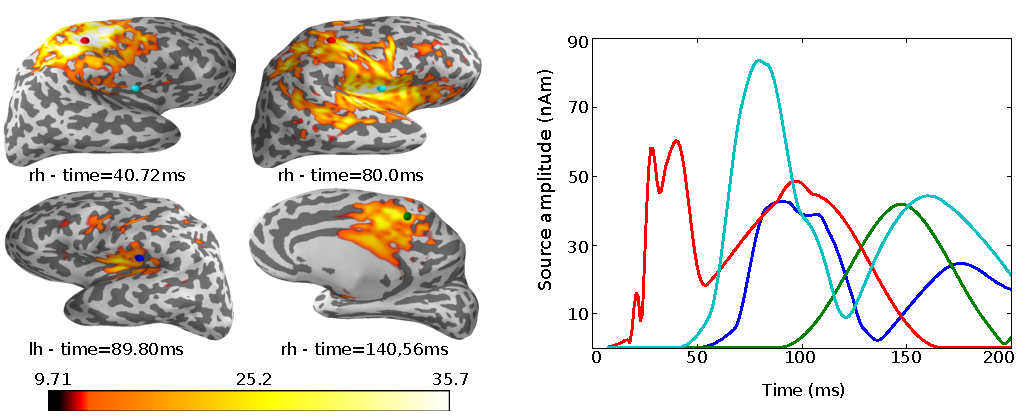
\includegraphics[width=0.95\textwidth]{multidict/fig_MEG}
    \caption{Source reconstruction using somatosensory data with a multi-scale irTF-MxNE. The solver estimates four sources for $\lambda_{space}=28.5$ and $\lambda_{time}=1.3$. The source locations marked with spheres in right (rh) and left (lh) hemisphere, and their corresponding activation are color-coded.}
	\label{fig:MEG}
\end{figure}

The multi-scale version of the MEG/EEG inverse problem in the TF domain does not only allow the capture of mixture of brain signals. An interesting point is the non-stationary aspect of the sources, which can be activated only for a short time window in a longer one. This multi-scale solver is then allowing us to analyze and reconstruct signals with variable characteristics over time. So far, all the results presented have been using a Gabor transform by fixing its window length and the time shift. The Gabor transform is a special case of STFT (the discrete case), and the question is what if this dictionary is not the best choice of where to decompose the data. The choice of the STFT was driven mostly by its flexibility of the choice of the dictionary being redundant or overcomplete. Moreover, its efficient implementation using fast FFT makes the STFT/iSTFT computation possible even with very redundant dictionaries.\\

\begin{figure*}
        \centering
        \begin{subfigure}[b]{0.48\textwidth}
            \centering
            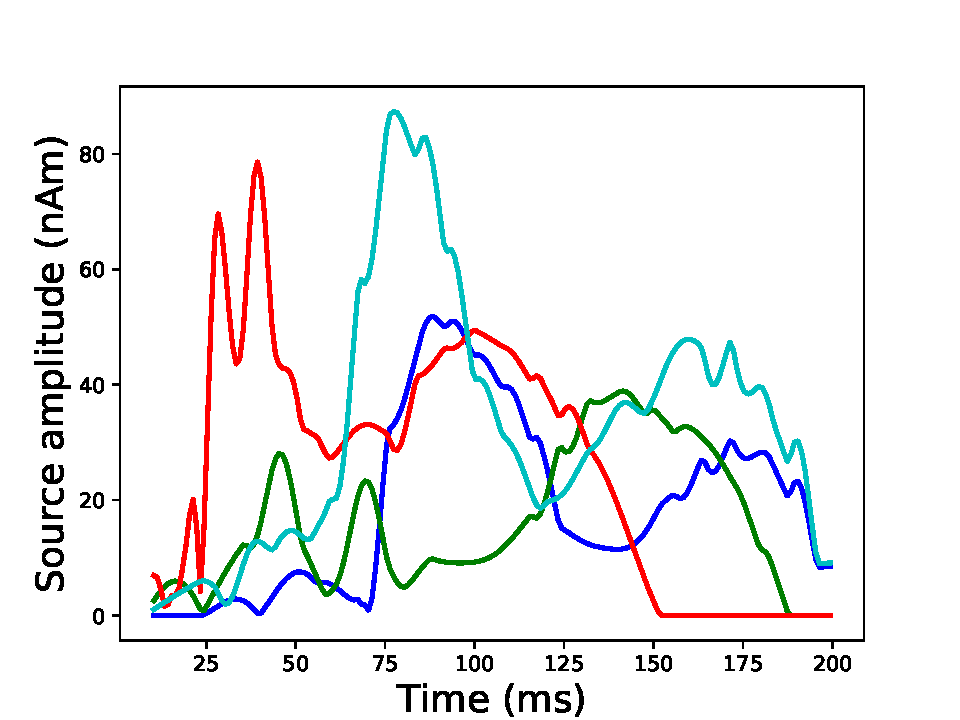
\includegraphics[width=\textwidth]{multidict/mdct_ws_64_16_tshift_32_8}
            \caption{MDCT: window size = 64-16,\\
            		    time shift = 32-8}
            \label{fig:mdct_short}
        \end{subfigure}
        \hfill
        \begin{subfigure}[b]{0.48\textwidth}  
            \centering 
            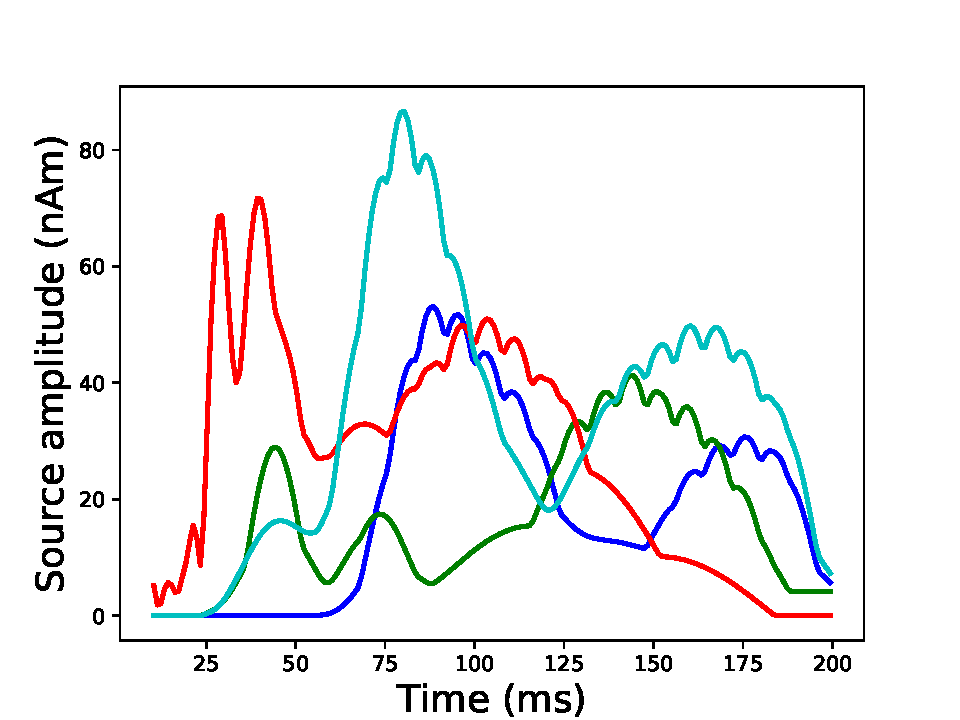
\includegraphics[width=\textwidth]{multidict/stft_ws_64_16_tshift_32_8}
            \caption{STFT: window size = 64-16,\\
            		    time shift = 32-8}
            \label{fig:stft_short}
        \end{subfigure}
        \vskip\baselineskip\vspace{-15pt}
        \begin{subfigure}[b]{0.48\textwidth}   
            \centering 
            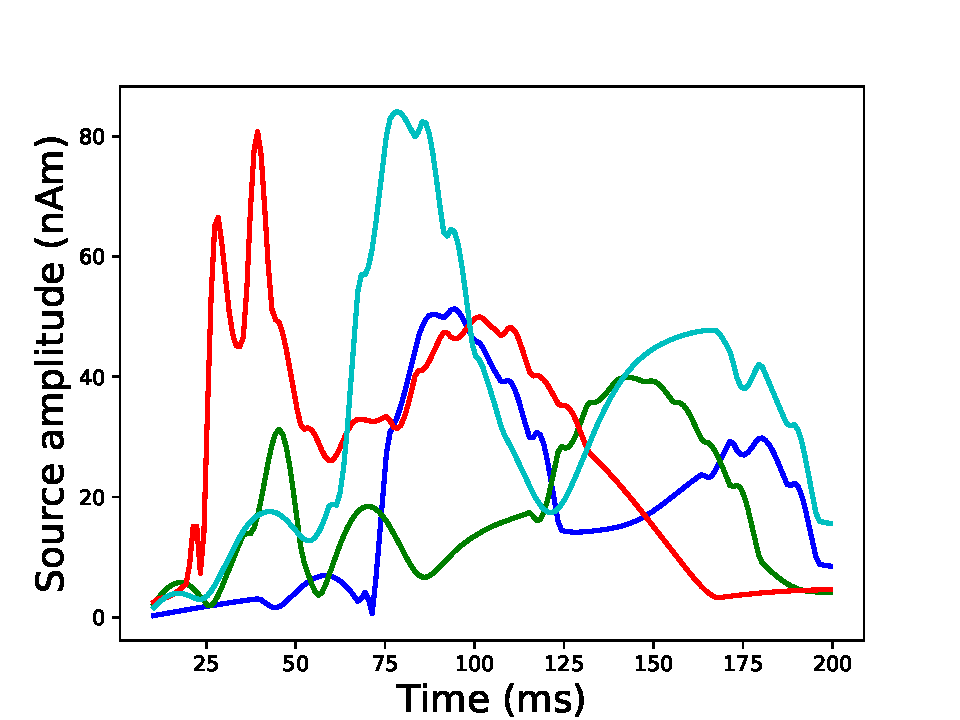
\includegraphics[width=\textwidth]{multidict/mdct_ws_128_16_tshift_64_8}
            \caption{MDCT: window size = 128-16,\\
            		    time shift = 64-8}
            \label{fig:mdct_long}
        \end{subfigure}
        \quad
        \begin{subfigure}[b]{0.48\textwidth}   
            \centering 
            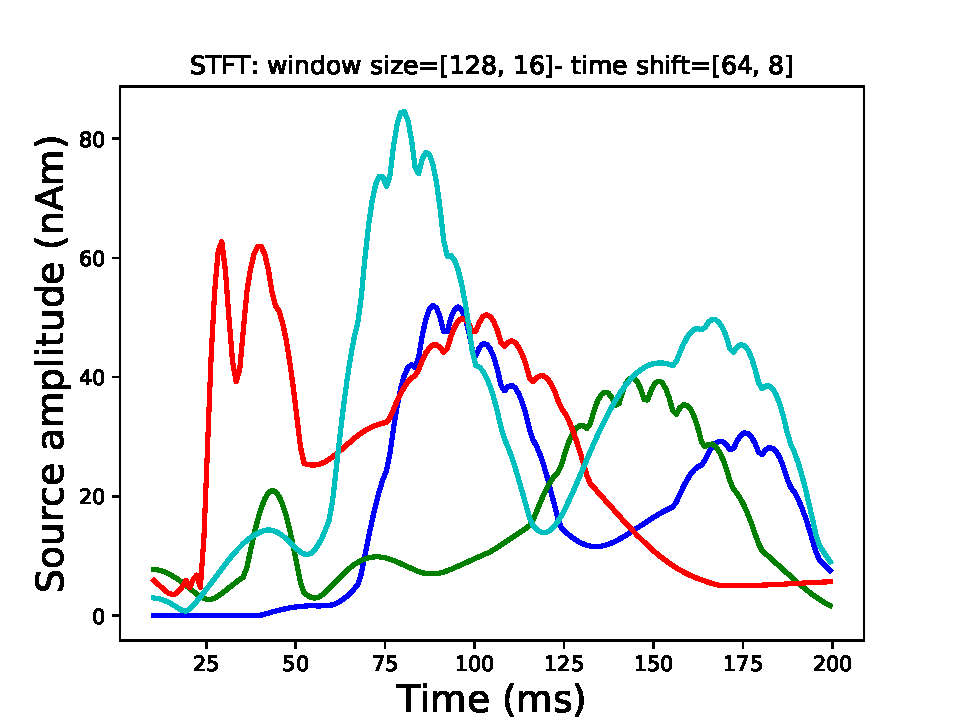
\includegraphics[width=\textwidth]{multidict/stft_ws_128_16_tshift_64_8}
            \caption{STFT: window size = 128-16,\\
            		    time shift = 64-8}
            \label{fig:stft_long}
        \end{subfigure}
        \vskip\baselineskip\vspace{-15pt}
        \begin{subfigure}[b]{0.48\textwidth}   
            \centering 
            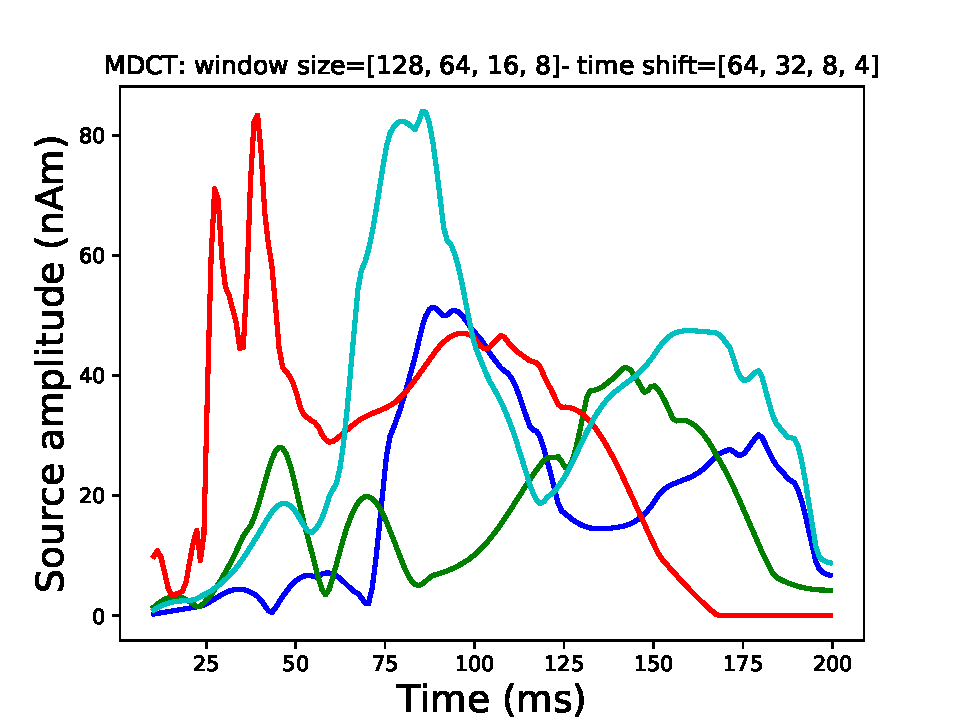
\includegraphics[width=\textwidth]{multidict/mdct_ws_128_64_16_8_tshift_64_32_8_4}
            \caption{MDCT: window size = 128-64-16-8,\\
            		    time shift = 64-32-8-4}
            \label{fig:mdct_all_dict}
        \end{subfigure}
        \quad
        \begin{subfigure}[b]{0.48\textwidth}   
            \centering 
            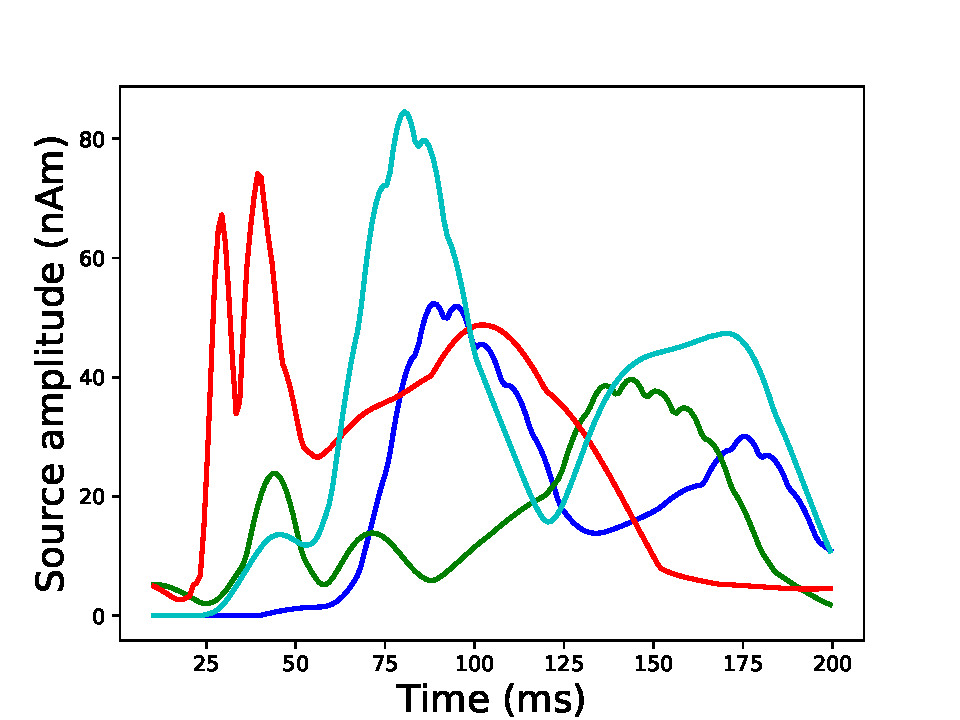
\includegraphics[width=\textwidth]{multidict/stft_ws_128_64_16_8_tshift_64_32_8_4}
            \caption{STFT: window size = 128-64-16-8,\\
            		    time shift = 64-32-8-4}
            \label{fig:stft_all_dict}
        \end{subfigure}
        \caption{Comparison between MDCT and STFT using Somatosensory of the MIND dataset. MDCT is shown in the left column and STFT on the right column.} 
        \label{fig:comparison_mind_mdct_stft}
\end{figure*}

We investigated a second choice: Modified Discrete Cosine Transform (MDCT). The problem found with MDCT is the fact that it is critically sampled. The sliding time windows are overlapping so that the last half of one block coincides with the first half of the next block, \textit{i.e.}, the time shift is equal to the half of the window's length. Figure~\ref{fig:comparison_mind_mdct_stft} shows several mixture of dictionaries for MDCT, but also for STFT if we set the time shift at half the window size. One can directly notice that it is harder to obtain both transient and smooth signals without any leakage between the time sources. MDCT is more sensitive to all the hyperparameters: the dictionary window length and the $\lambda_{space}$/$\lambda_{time}$. Even if we leave in a side the compromise that one needs to keep in mind between the size of multi-scale dictionary and the computation time by having multiple dictionaries concatenated together as in Figure~\ref{fig:comparison_mind_mdct_stft}-\ref{fig:mdct_all_dict}, MDCT is still not able to be comparable to STFT as in Figure~\ref{fig:MEG}.

\section{Conclusion \& Perspective}
In this chapter, the main motivation of the multi-scale dictionary has been presented. The first contribution has been presented which improves the irTF-MxNE solver using a multi-scale dictionary to capture the mixture of the MEG/EEG data. The non-convex optimization problem is solved by iteratively solving the convex weighted TF-MxNE problem using block coordinate descent combined with active set strategy to speed up the convergence.

The benefits of the multi-scale irTF-MxNE have been shown on simulated and MEG somatosensory data. Both experiments confirm that multi-scale irTF-MxNE improves the source estimates, in terms of reduced mixing of the time courses, smoothness and detection of both short transients and slower waves. In contrast, both solvers are efficient regarding active set size and amplitude bias, which is due to the non-convexity of the methods. Hence, the multi-scale irTF-MxNE should be applied to data where a mixture of signals coexist, and when the aim is to acquire focal sources with non-stationary and smooth time courses.

 % (https://www.researchgate.net/publication/301731870_Brain_reading_with_ordered_targets_using_ranking_metric).

Further work related to this chapter can address different points:
\begin{itemize}
%    \item Multi-scale irTF-MxNE investigation in terms of dictionary. So far we have used tight Gabor frames, is it the best choice? Doing some \textit{"exhaustive"} comparison between the STFT used here, Modifed Discrete Cosine Transform (MDCT), and Stockwell transform \textit{a.k.a.} S-Transform will help us better understand the dictionary decomposition of the data.
	\item Multi-scale irTF-MxNE improvement in terms of hyperparameter learning, \textit{i.e.} estimation of the best parameters $\lambda_{space}$ and $\lambda_{time}$. In the standard cases, these parameters are selected by cross-validation or sometimes by using the discrepancy principle. A key contribution in this direction would be to use Bayesian inference techniques to estimate those regularization parameters in a composite norms setting.
    
    \item The source localization in general is computed over an \textit{evoked}, \textit{i.e.} in the MEG/EEG field, the evoked is the mean of several trials of the same experiment. The main purpose is to reduce the noise, \textit{i.e.}, increase the SNR of the signal. At a trial level, \textit{i.e.}, for a lower SNR, how can we improve the source localization? We can constraint the localization with the prior knowledge that all trials are supposed to have the same source estimate.
    
    \item Optimization direction, the idea of incorporating screening techniques presented in a huge amount of papers can help to speed up the convergence, and so the reconstruction time\cite{massias2017safe,massiasgap,fercoq-etal:2015,Ndiaye_Fercoq_Gramfort_Salmon15,ndiaye2016gap,ndiaye2017efficient}.
\end{itemize}


% Chapter 3

\chapter{The Bayesian approach: Hierarchical Bayesian modeling}
\label{chapter:bayesian}
\noindent\makebox[\linewidth]{\rule{0.75\paperwidth}{0.4pt}}
\noindent\makebox[\linewidth]{\rule{0.75\paperwidth}{0.4pt}}

\localtableofcontents % local toc

\noindent\makebox[\linewidth]{\rule{0.75\paperwidth}{0.4pt}}
\noindent\makebox[\linewidth]{\rule{0.75\paperwidth}{0.4pt}}

\newpage

%----------Intro - general concepts --------------------------------------------------------
\section{Introduction - General concepts}
\label{sec:bayes_intro}
%%%%%%%%%%%%%%%%%%%%%%%%%%%%%%%%%%%%%%%%%%%%%%%%%%%%%%%%%%%%%%%%%%%%%%%%%%%%%%%

This chapter presents a novel way to look at the MEG/EEG inverse problem. It tries to gap the bridge between two communities both interested in the sparse models of inverse problems. As mentioned several times so far in this thesis, sparsity has emerged as a key concept to solve inverse problems not onlyt the MEG/EEG inverse problem, but also as tomographic image reconstruction, deconvolution or inpainting. The idea is to regularize high dimensional regression problems in the field of machine learning. There are mainly two routes to introduce sparsity to such problems.

The first route, embraced by the optimization community and frequentist
statisticians, is to promote sparsity using convex optimization theory.
This line of work has led to now mature theoretical guarantees~\cite{FoRa13} when using regularization functions based on $\ell_1$ norm and other convex variants~\cite{Tibshirani96}. In particular, it has been popularized in the signal processing community under the name of compressed sensing~\cite{candes2008introduction} when combined with incoherent measurements.

There are however some limitations of sparsity promoting convex penalties based on the $\ell_1$ norm.
All the features (also called regressors, atoms or sources depending on the terminology of the community) involved in the solution form what is called the support of the solution.
Convex penalties can fail to identify the correct support in the presence of highly noisy data, but also in low noise setups if the forward operator (referred to as design matrix in statistics) is poorly conditioned. Convex regularizations also leads to a systematic underestimation bias in the amplitude of the coefficients~\cite{OsBuGoXuYi06,Candes,chartrand2007exact,saab2008stable,ChHeSa17}.

To address these limitations of $\ell_1$-type models, reweighted schemes have been proposed~\cite{Candes,Gasso,Rakotomamonjy,zhang-rao:2011,strohmeier-etal:16}, of which the Adaptive Lasso~\cite{Zou06} is the most commonly used in the statistics community: Starting from the Lasso estimator, which amounts to regressing with a standard $\ell_1$-norm as a regularizer (this estimator is sometimes referred to as Basis Pursuit Denoising (BPDN)~\cite{Chen_Donoho_Saunders98} in signal processing), the Adaptive Lasso solves a sequence of weighted Lasso problems, where at each iteration the weights are chosen such that the strongest coefficients are less and less penalized.
From the optimization point of view, such an iterative scheme can be derived from so-called majorization-minimization (MM) strategies~\cite{lange2000optimization,schifano2010majorization}.
The idea behind MM is to minimize the objective function by successively minimizing upper bounds that are easier to optimize. Many well-known optimization approaches can be interpreted as instances of MM, \eg simple gradient descent or proximal algorithms~\cite{Combettes2011}, expectation-maximization (EM)~\cite{Dempster77maximumlikelihood}, and difference-of-convex (DC) programming techniques~\cite{Horst:1999}.
%
More recently, re-weighted $\ell_1$-norm schemes based on MM principle have been particularly popular to handle concave, hence non-convex regularizations such as $\ell_{0.5}$-quasi-norms or logarithmic functions. As such, these schemes are prone to converging to a local minimum determined by the initial, uniformly weighted $\ell_1$-norm solution (\ie the Lasso estimator) that constitutes the first iterate. This first route has been defined in more details in Chapter~\ref{chapter:background} and Chapter~\ref{chapter:multiscale}.

The second route to introduce sparsity formulates the regression problem in a Bayesian framework and uses hierarchical Bayesian models (HBM) \cite{mackay2003information} for the inference.
The common way to formulate HBMs is to consider the variance parameters of Gaussian prior models as additional random variables which have to be estimated from the data as well. Their prior distributions are referred to as hyper-priors. Plausible solutions to the regression problem that both fit data and the \emph{a priori} assumption of sparsity are explicitly characterized as multiple distinct modes of the posterior distribution. This characterization is the Bayesian analogue to local minima in variational regression approaches when working with non-convex functionals. Different strategies to infer a point estimate for the parameters of interest from the \emph{a posteriori} distribution then lead to different algorithmic frameworks, for instance Variational Bayesian approaches~\cite{mackay2003information,jordan1999introduction,sato2004hierarchical,FrHaDaKiPhTrHeFlMa08,shervashidze2015learning}, Sparse Bayesian Learning (SBL) approaches (also referred to as type-I or type-II maximum likelihood estimates) \cite{tipping2001sparse,wipf2004sparse,Wipf-Nagarajan:2009,zhang-rao:2011} and fully-Bayesian strategies \cite{CaHaPuSo09,Lucka-etal:2012}.

This chapter focuses on the later one for a non-standard type of HBM examined in \cite{Lu14} that combines a non-Gaussian prior with an $\ell_{1}$-type energy function with a specific Gamma hyper-prior.
For this HBM, a simple alternating scheme to compute full maximum \emph{a posteriori} (MAP) estimates leads to exactly the same sequence of problems solved by MM applied to $\ell_{1/2}$-type regularizations.
With this observation made, it is natural to revisit and improve these MM schemes by leveraging the ability of the Bayesian framework to explore the modes of the posterior distribution by Markov chain Monte-Carlo (MCMC) schemes \cite{RoCa05,KaSo05}. This can not only mitigate the aforementioned initialization-dependence of MM, but more importantly, it offers insights into the structure and importance of potentially multiple plausible sparse solutions. Yet, the benefit comes at the cost of additional computational efforts.

This chapter is organized as follows: First, it presents in a unified
perspective on both routes to sparsity, \ie reweighted $\ell_1$ MM schemes
and specific HBMs. We show that a particular optimization-based inference strategy recovers the MM algorithm. it then describes an HBM inference strategy based upon an MCMC sampling and show on simulated and experimental M/EEG datasets how these stochastic MCMC-based techniques can not only help to improve upon deterministic approaches but also help to reveal multiple plausible solutions to the inverse problem. This analysis leads to an uncertainty quantification (UQ) of the support recovery of non-convex sparse regression problems that provides very useful complementary information, in particular for very ill-conditioned and under-determined applications like MEG/EEG source localization.

%----------Lp hypermodels ------------------------------------------------------------------
\section{Lp hyper-models}

%----------MAP estimation ------------------------------------------------------------------
\section{MAP estimation}

%----------Link between MM & HBM------------------------------------------------------------
\section{Link between MM and special case of HBM}

We start this section by recalling how majorization-minimization works
when addressing variational formulations with concave, hence non-convex, regularization.
It is followed by an introduction to hierarchical Bayesian models with Gamma hyper-priors.
Then, we explain how these seemingly different approaches can lead to the
exact same regression algorithm.
From this, we detail how different Bayesian inference strategies using MCMC
sampling can more precisely explore the landscape of the posterior distribution of the HBM model and provide multiple possible solutions to the sparse regression problem compared to MM.

\subsection{Majorization-Minimization: MM}
\label{section:MM}

Majorization-Minimization (MM) strategies consist in replacing a difficult optimization problem with a series of easier ones that are obtained by upper bounding the objective function, often by a convex majorant.
%
In the context of inverse problems or high-dimensional statistics using sparsity constraints, MM has been successfully applied to address non-convex regularization terms. An example is the regression model with $\ell_{2,p}$-quasi-norms regularization over the groups when $0<p<1$: the desired estimate $\hat{\bfX}$ is defined as one of potentially multiple minimizers of:

\begin{equation} \label{eq:L2pReg}
\hat{\bfX} \in \argmin_{\bfX\in\R^{SO \times T}} \frac{1}{2} \fronormsq{\bfM - \bfG \bfX}  + \lambda \sum_{i=1}^S \fronorm{\bfX{[i]}}^p \enspace,
\end{equation}
where $\lambda > 0$ is the regularization parameter balancing the data fit and the penalty term. One possible MM approach to solve Equation~\eqref{eq:L2pReg} with $p=0.5$ would consist of minimizing a sequence of non-smooth convex surrogate functions where the non-convex regularization (irMXNE solver) is replaced by a weighted $\ell_{2,1}$ norm similar to MxNE solver~\cite{strohmeier-etal:16}. In each iteration, the weights are derived from the current estimate of $\bfX$.

Due to the concavity of the non-decreasing function $\bfX\mapsto\sqrt{\fronorm{\bfX}}$, it is upper bounded by its tangent and a first order Taylor expansion at the current estimate $\bfX{[i]}$ provides an upper bound that can be used to construct the non-smooth convex surrogate problem. By solving this sequence of surrogate problems, the value of the non-convex objective function is guaranteed to decrease. However, due to the non-convexity, only convergence towards a local minimum can be guaranteed.

For the problem in Equation~\eqref{eq:L2pReg} with $p=0.5$, the $k^{th}$ iteration of the MM scheme reads:
\begin{equation}
\label{eq:MM}
\fl \quad \bfX^{(k)} \in \argmin_{\bfX\in\R^{SO \times T}} \frac{1}{2} \fronormsq{\bfM - \bfG \bfX}  + \lambda \sum_{i=1}^S \frac{ \fronorm{\bfX{[i]}} }{ \bfw^{(k-1)}[i]},
\end{equation}
with:
\begin{equation*}
\bfw^{(k-1)}[i] = 2 \sqrt{\fronorm{\bfX^{(k-1)}[i]}} \enspace.
\end{equation*}
As each weight $\bfw^{(k)}[i]$ is a non-decreasing function of $\fronorm{\bfX^{(k)}[i]}$, sources with high amplitudes in one iteration will be less penalized in the next iteration and can better explain the data $\bfM$. Sources for which $\fronorm{\bfX^{(k)}[i]} = 0$ at a certain iteration $k$ are effectively pruned from the model for all following iterations. Using MM therefore leads to a solution that explains the data with fewer active locations $i$ compared to a standard $\ell_{2,1}$ norm regularized solution.\\
Note that a default initialization consists in setting $\bfw^{(0)}[i]=1, \forall i \in [1,\cdots, S]$~\cite{strohmeier-etal:16}.

To exploit existing fast solvers for the $\ell_{2,1}$ regularized problems~\cite{strohmeier-etal:16,Ndiaye_Fercoq_Gramfort_Salmon15}, we reformulate the weighted subproblem and apply the weights by scaling the matrix $\bfG$ with a diagonal matrix $\bfW^{(k)} \in \bbR^{SO \times SO}$ given by:
\begin{eqnarray} \label{eq:weights}
\bfW^{(k)} = \mathrm{diag}(\bfw^{(k)} \otimes \mathbf{1}_{O}) \enspace ,
\end{eqnarray}
where $\bfw^{(k)} \in \bbR^{S}$, $\mathbf{1}_{O}\in\R^O$ is a vector of ones and $\otimes$ is the Kronecker product.
Defining $\tilde{\bfG}^{(k)}=\bfG \bfW^{(k-1)}$, the reformulated problem reads:
\begin{eqnarray}\label{eq:lasso_new_gram}
\tilde{\bfX}^{(k)} \in \argmin_{\bfX\in\R^{SO \times T}} \frac{1}{2}\fronormsq{\bfM - \tilde{\bfG}^{(k)} \bfX}  + \lambda \sum_{i=1}^S \fronorm{\bfX[i]} \enspace .
\end{eqnarray}

The convergence of each weighted $\ell_{2,1}$ (MxNE) is controlled by monitoring the duality gap (see Section~\ref{section:duality_gap}). For more details about convex duality of optimization with sparsity-inducing sparsity, refer to~\cite{bach2012optimization}.\\
As mentioned in Section~\ref{section:duality_gap}, the minimum of the primal objective function $f_p(\mathbf{X})$ is bounded below by the maximum of the dual objective function $f_d(\mathbf{Y})$, \textit{i.e.},\\
$f_d(\mathbf{Y}^\star)\leq f_p(\mathbf{X}^\star)$ where $\mathbf{X}^\star$ and $\mathbf{Y}^\star$ are the optimal solutions of the primal and the dual objective functions respectively. If strong duality holds, the duality gap defined as $\eta=f_p(\mathbf{X})-f_d(\mathbf{Y})$ would be zero at the optimum.\\
Due to Slater's conditions~\cite{Boyd_Vandenberghe04}, strong duality gap holds for MxNE subproblem to check the convergence of Equation~\eqref{MM}. Based on Fenchel-Rockafellar duality theorem~\cite{rockafellar:1997}, the dual objective function associated with the primal objective function:
\begin{equation}
\begin{split}
f_p(\mathbf{X}) & = \frac{1}{2}\|\mathbf{M}-\mathbf{GX}\|_{Fro}^2+\lambda\mathcal{P}(\mathbf{X}) \\
& = \frac{1}{2}\|\mathbf{M}-\mathbf{GX}\|_{Fro}^2+\lambda\sum_{i=1}^S\|\mathbf{X}[i]\|_{Fro}
\end{split}
\end{equation}
is given by:
\begin{equation}
f_d(\mathbf{Y})=-\frac{1}{2}\|\mathbf{Y}\|_{Fro}^2+Tr(\mathbf{Y}^\top\mathbf{M})-\lambda\mathcal{P}^\star(\mathbf{G}^\top\mathbf{Y}/\lambda)
\end{equation}
where $\mathcal{P}^\star$ is the Fenchel conjugate of $\mathcal{P}$, which is the indicator function of the associated dual form. For a full derivation, see~\cite{Gramfort_Kowalski_Hamalainen12}. Moreover, the Karush-Khun-Tucker (KKT) conditions of the Fenchel-Rockafellar duality theorem give a natural from
the primal to the dual space, which is given by a scaling of the residual $\tilde{\mathbf{Y}}=\mathbf{M}-\mathbf{GX}$, as shown in~\cite{Gramfort_Kowalski_Hamalainen12}.\\
In practice, we terminate the optimization scheme for solving MxNE when the estimate at the $k^{th}$ iteration is $epsilon$-optimal with $\epsilon=10^{-6}$~\cite{strohmeier-etal:16}.\\

{\fontsize{4}{4}\selectfont
%above is to make smaller fonts in algorithm
\begin{algorithm}[t]
\SetKwInOut{Input}{input}
\SetKwInOut{Init}{init}
\SetKwInOut{Parameter}{param}
\caption{\textsc{$\ell_{2,p}$ MM algorithm with $p=0.5$ (Adaptive Lasso) - iterative reweighted MxNE}}
\Input{$\bfM, \bfG,\lambda > 0, \bfW^{(0)} \geqslant 0,\epsilon > 0, \tau > 0$ and $K$ }
% \Parameter{ To add }
%\Init{$\bfW^{(1)}=I_{dn\times dn}$ }
\For{
        $k = 1$ to $K$
    }
    {
		$\tilde{\bfG}^{(k)} = \bfG \bfW^{(k-1)}$

		Get $\tilde{\bfX}^{(k)}$ solving Equation~\eqref{eq:lasso_new_gram} at $\epsilon$-precision as done in Algorithm~\ref{alg:mxne_activeset}.

		Update $\hat{\bfX}^{(k)} = \bfW^{(k-1)} \tilde{\bfX}^{(k)}$

	    Update $\bfW^{(k)}=\mathrm{diag}(\bfw^{(k)} \otimes \mathbf{1}_{O})$ where $\bfw^{(k)}[i] = 2 \sqrt{\fronorm{\hat{\bfX}^{(k)}[i]}}$,  $\forall i\in [1, cdots, S]$

		\If{ $\norm{\hat{\bfX}^{(k)}-\hat{\bfX}^{(k-1)}}_{\infty} \leq \tau$}{Break}

     }
%\Return{$\hat{\bfX}^{(k)}$}
\label{alg:adpative_lasso}
\end{algorithm}
}

For solving the weighted MxNE subproblems, a block coordinate descent (BCD) scheme was used~\cite{tseng}, which for the problem at hand converges faster than the Fast Iterative Shrinkage Thresholding Algorithm (FISTA) (See Section~\ref{section:comparison_solvers}). The subproblem per block has a closed form solution, which involves applying the group soft-thresholding operator, the proximity operator associated to the $\ell_{2,1}$-mixed-norm~\cite{gramfort2012mixed,strohmeier-etal:16}.

{\fontsize{4}{4}\selectfont
%above is to make smaller fonts in algorithm
\begin{algorithm}[t]
\SetKwInOut{Input}{input}
\SetKwInOut{Init}{init}
\SetKwInOut{Parameter}{param}
\caption{\textsc{MxNE with BCD and active set strategy}}
\Input{$\bfM, \bfG,\lambda > 0, \epsilon > 0$, and $S$ }
% \Parameter{ To add }
\Init{$\mathbf{X}=0$, $\Gamma=\{\}$, $\eta=f_p(\mathbf{X})-f_d(\mathbf{Y})$}
\For{
        $i = 1$ to $S$
    }
    {
		$\mu[i] = \|\mathbf{G^\top_i\mathbf{G}_i}\|^{-1}$
     }
\While{
		$\eta \geq \epsilon$
	  }
	  {
	  	$\Gamma^\star\subseteq \{i \hspace{3pt} | \hspace{3pt} \|\mathbf{G}_i^\top(\mathbf{M}-\mathbf{GX})\|_{Fro} > \lambda\}$

	  	$\Gamma = \Gamma\cup \Gamma^\star$

	  	Define $\mathbf{G}^\Gamma$ and $\mathbf{X}^\Gamma$ by restricting $\mathbf{G}$ and $\mathbf{X}$ to $\Gamma$

	  	$\mathbf{X}^{\star\Gamma}\leftarrow$ Solve Algorithm~\ref{alg:} with $\mathbf{\mu}, \mathbf{G}^\Gamma$, and $\mathbf{X}_0=\mathbf{X}^\Gamma$

	  	$\mathbf{X}=\mathbf{X}^{\star\Gamma}$ for $i\in\Gamma$, else 0

	  	$\eta=f_p(\mathbf{X})-f_d(\mathbf{Y})$
	  }
%\Return{$\hat{\bfX}^{(k)}$}
\label{alg:mxne_activeset}
\end{algorithm}
}

{\fontsize{4}{4}\selectfont
%above is to make smaller fonts in algorithm
\begin{algorithm}[t]
\SetKwInOut{Input}{input}
\SetKwInOut{Init}{init}
\SetKwInOut{Parameter}{param}
\caption{\textsc{MxNE with BCD}}
\Input{$\bfM, \bfG,\bfX, \mathbf{\mu}, \lambda > 0, \epsilon > 0$, and $S$ }
% \Parameter{ To add }
\Init{$\eta=f_p(\mathbf{X})-f_d(\mathbf{Y})$}
\While{
		$\eta \geq \epsilon$
	  }
	  {
	  	\For{
	  			$i=1 in S$
	  		}
	  		{
	  			$\mathbf{X}[i]\leftarrow$ Solve Equation~\eqref{eq:} with $\mathbf{X}, \mathbf{\mu}$, and $\mathbf{M}$
	  		}
	  	$\eta = f_p(\mathbf{X})-f_d(\mathbf{Y})$
	  }
\label{alg:mxne_bcd}
\end{algorithm}
}

After convergence, we reapply the scaling to $\tilde{\bfX}$ to obtain $\hat{\bfX}$:
\begin{equation}
    \label{eq:MM_weights}
    \bfX^{\star(k)} = \bfW^{(k-1)} \tilde{\bfX}^{(k)} \enspace .
\end{equation}
The reformulation through Equation~\eqref{eq:lasso_new_gram} and Equation~\ref{eq:MM_weights} avoids any division by zero when $\bfX^{(k-1)}=0$. The above procedure, which matches the strategy of the Adaptive Lasso estimator~\cite{Zou06}, is expressed as pseudo-code in Algorithm~\ref{alg:adpative_lasso}.

%%%%%%%%%%%%%%%%%%%%%%%%%%%%%%%%%%%%%%%%%%%%%%%%%%%%%%%%%%%%%%%%%%%%%%%%%%%%%%%
\subsection{Hierarchical Bayesian Modeling}
\label{section:HBM}
%%%%%%%%%%%%%%%%%%%%%%%%%%%%%%%%%%%%%%%%%%%%%%%%%%%%%%%%%%%%%%%%%%%%%%%%%%%%%%%

In this section, we formulate the inference problem given by Equation~\eqref{eq:FwdEq} and the regularization strategy with $\ell_{2,p}$-quasi-norms from a Bayesian perspective~\cite{KaSo05,Lu14}: the Bayesian approach incorporates prior beliefs about the model parameters in terms of probability distributions. Under the additive, white Gaussian noise (AWGN) assumption the likelihood of the model is given by:
\begin{eqnarray} \label{eq:like}
\like &\propto \exp \left( - \frac{1}{2} \fronormsq{\bfM - \bfG \bfX} \right) \enspace.
\end{eqnarray}

From Equation~\eqref{eq:L2pReg} we can construct the $\ell_{2,p}$ group prior as:

\begin{equation} \label{eq:prior}
\prior \propto \exp \left( - \lambda \sum_{i=1}^S \fronorm{\bfX[i]}^p \right)
= \prod_{i=1}^S \exp \left( - \lambda \fronorm{\bfX[i]}^p \right) \enspace,
\end{equation}

which leads to the following posterior probability density using the Bayes rule:

\begin{equation} \label{eq:post}
\post \propto \exp \left( - \frac{1}{2} \fronormsq{\bfM - \bfG \bfX} - \lambda \sum_{i=1}^S \fronorm{\bfX[i]}^p \right) \enspace.
\end{equation}

To extend Equation~\eqref{eq:prior} to a hierarchical prior model~\cite{mackay2003information}, the scalar $\lambda$ has been replaced by a vector of hyperparameters $\mathbf{\gamma} \in \R^{S}_+$ and for any $p \geq 1$ we write the \emph{conditional $\ell_{2,p}$ prior} as:
\begin{equation} \label{eq:condprior}
\fl \hiprior
\propto \exp \left( - \sum_{i=1}^S \left( \frac{\fronorm{\bfX[i]}^p}{\mathbf{\gamma}[i]} + \frac{O T}{p} \log(\mathbf{\gamma}[i])\right)\right) \enspace,
\end{equation}
where the logarithmic term accounts for the terms of the normalization that depend on $\mathbf{\gamma}$~\cite{Lu14}. A common choice for a hyper-prior on each $\gamma[i]$ is given by a \emph{Gamma distribution}~\cite{mackay2003information,KaSo05,CaHaPuSo09,Lucka-etal:2012} with shape and scale parameters $\alpha$ and $\beta$:
\begin{align} \label{eq:hyper}
\fl \hyper & \propto \prod_{i=1}^S \mathbf{\gamma}[i]^{\alpha - 1} \exp \left(- \frac{\mathbf{\gamma}[i]}{\beta} \right) \\
& = \exp \left( - \sum_{i=1}^S \left( - \frac{\mathbf{\gamma}[i]}{\beta} + (\alpha - 1) \log(\mathbf{\gamma}[i]) \right) \right) \enspace.
\end{align}
Then, the full posterior over both $\bfX$ and $\gamma$ becomes:
\begin{eqnarray}
\label{eq:full-post}
\fl \hipost \propto \nonumber \\
\fl \hspace{3em} \exp \left( - \frac{1}{2} \fronormsq{\bfM - \bfG \bfX} - \sum_{i=1}^S \left( \frac{\fronorm{\bfX[i]}^p}{\mathbf{\gamma}[i]} + \frac{\mathbf{\gamma}[i]}{\beta} - (\alpha - 1 - \frac{OT}{p}) \log(\mathbf{\gamma}[i]) \right) \right)\enspace.
\end{eqnarray}
The question of how to best derive parameter estimates, in particular how to treat the two different types of parameters $\bfX$ and $\mathbf{\gamma}$, distinguishes different HBM-based inference strategies. Variational Bayesian approaches~\cite{mackay2003information,jordan1999introduction,sato2004hierarchical,FrHaDaKiPhTrHeFlMa08,shervashidze2015learning} and Sparse Bayesian Learning~\cite{tipping2001sparse,wipf2004sparse,Wipf-Nagarajan:2009,zhang-rao:2011} approaches rely on approximating or marginalizing the full, joint posterior distribution (Equation~\eqref{eq:full-post}). In contrast, fully-Bayesian strategies~\cite{CaHaPuSo09,Lucka-etal:2012} work with it directly. The most popular one is the full maximum-a-posteriori (\emph{full-MAP}) estimate which is defined as:

\begin{eqnarray}
(\xMAP,\gamMAP) & \in \argmax_{(\bfX,\mathbf{\gamma}) \in\R^{SO \times T} \times \R^{n}_+} \left\lbrace \hipost \right\rbrace \enspace.%,\\
\end{eqnarray}
A common strategy  to compute it is to minimize the \emph{negative log posterior} $-\log \hipost$ by alternating  minimization over $\bfX$ and $\mathbf{\gamma}$ (\emph{block coordinate descent} in optimization):

\begin{equation}\label{eq:AO-X}
\fl \qquad  \bfX^{(k)} \in \argmin_{\bfX\in\R^{SO \times T}} \left\lbrace \frac{1}{2} \fronormsq{\bfM - \bfG \bfX} + \sum_{i=1}^S  \frac{\fronorm{\bfX[i]}^p}{\mathbf{\gamma}^{(k-1)}[i]} \right\rbrace \enspace,
\end{equation}
\begin{equation}\label{eq:AO-gamma}
\begin{split}
\fl \qquad \mathbf{\gamma}^{(k)}[i] \in \argmin_{\mathbf{\gamma}[i]\in \R_+} & \left\lbrace\frac{\fronorm{\bfX^{(k)}[i]}^p }{\mathbf{\gamma}[i]} + \frac{\mathbf{\gamma}[i]}{\beta} - (\alpha - 1 - \frac{OT}{p}) \log(\mathbf{\gamma}[i]) \right\rbrace, \\
& \forall i\in [1,\cdots, S] \enspace. 
\end{split}
\end{equation}
Other fully-Bayesian estimates are defined as integrals of functions of $\bfX$ and $\mathbf{\gamma}$ with respect to the posterior distribution, \textit{e.g.} first or second moment estimates. To compute these high dimensional integrals efficiently, only Markov chain Monte-Carlo (MCMC) methods that draw correlated samples from the posterior distribution can be used\cite{RoCa05,KaSo05} . A commonly used MCMC scheme for HBM is given by \emph{blocked Gibbs sampling} which alternates as:
\begin{eqnarray}
\bfX^{(k)} &\sim \: p_{post}(\bfX,\mathbf{\gamma}^{(k-1)}|\bfM) &\propto p_{post}(\bfX|\bfM,\mathbf{\gamma}^{(k-1)}) \enspace, \label{eq:AS-X}\\
\mathbf{\gamma}^{(k)} &\sim \: p_{post}(\bfX^{(k)},\mathbf{\gamma}|\bfM) &\propto p_{post}(\mathbf{\gamma}|\bfM,\bfX^{(k)})\enspace. \label{eq:AS-gamma}
\end{eqnarray}
Depending on the purpose of the study, here the main interest is not sampling the posterior distribution for computing the integral-based estimators but we rather want to explore the different modes of this multi-modal distribution, each of which corresponds to parameters that are both sparse and likely to explain the data.\\
One can notice similar structures in Equation~\eqref{eq:AO-X}-\eqref{eq:AO-gamma} and Equation~\eqref{eq:AS-X}-\eqref{eq:AS-gamma}: in each step, we make use of the conditional structure of the posterior: for $\mathbf{\gamma}$ fixed, we have to solve one $SOT$-dimensional $\ell_{2,p}$ optimization/sampling problem, while for $\bfX$ fixed, we have to solve $S$ 1-dimensional optimization/sampling problems. These two steps will be described in more detail in the sections~\ref{section:hbm_optim} and~ \ref{section:hbm_sampling}.

%----------hyperparam estimation------------------------------------------------------------
\section{Hyperparameter estimation in the variational formulation}
%%% Intro from Hyperparam paper

Before emphasizing the details of a full Bayesian formulation, this chapter also investigates the estimation of the hyperparamter $\lambda$ in the variational formulation. One can notice that hyperparameter setting is a classical statistics problem for which a number of solutions have been proposed. In signal processing, the AIC and BIC criteria are quite popular techniques historically~\cite{schwarz1978estimating}. The SURE-based techniques~\cite{stein1981estimation} have also been quite popular and recently explored for denoising and compressed sensing applications~\cite{luisier2007new, guo2015near}. In a standard supervised machine learning setup with independent and identically distributed (i.i.d.) observations, cross-validation (CV) is the reference approach. 
Also, the Bayesian approach suited for probabilistic models offers a principled way to estimate hyperparameters using hyperpriors that introduce softer constraints than solutions with fixed parameter values. This benefit yet usually comes at a price in terms of computational cost. Finally, in a number of real scenarios, humans end up setting hyperparameters, as they can have some expert knowledge that can correct model mismatch.

In statistical machine learning an hyperparameter typically aims at limiting overfitting by controlling the model complexity. In the particular case of regularized regression, classically a scalar parameter balances between the data fit and the penalty term. When using sparse regression, this parameter affects the sparsity of the solution, \emph{i.e.}, how many covariates or regressors are used.

With CV, some independent observations are left out of the inference and the
hyperparameter values that yield the best prediction performance on this data are selected. A search for the best parameter can be done with a time consuming exhaustive grid-search, smooth optimization (see \cite{pedregosa2016hyperparameter} and references therein), sequential or even random search~\cite{bergstra2011algorithms, bergstra2012random}. The CV approach however needs the i.i.d. assumption to be fulfilled, which is not always the case in practice, e.g. when working with signals or arrays of sensors as in the case of our application to brain imaging.

To keep it as a hierarchical Bayesian model problem and following a recent paper of Pereyra~\cite{Figueiredo}, we consider a HBM and propose to use a maximum-a-posteriori (MAP) estimation for the hyperparameters.

This thesis is particularly interested in the high-dimensional regression setting using group-Lasso-like structured sparsity as seen so far. In the literature a number of approaches have been proposed and MAP estimates that boil down to penalized regression with smooth or non-smooth penalties are the standard approaches employed by neuroscientists~\cite{haufe2008combining,ou2009distributed, bolstad2009space, wipf2009unified,gramfort2012mixed,lucka2012hierarchical,valdes2009eeg}.

In a variational formulation, the value of the hyperparameter $\lambda$ depends on the problem at hand, the noise level, and on the choice of regularization $\mathcal{P}(\mathbf{X})$.
Finding a way to estimate the hyperparameter with minimal user intervention is therefore particularly important, as it makes a comparison between different models and regularization easier.

Recently \textit{Pereyra et al.} \cite{Figueiredo} proposed a strategy for hyperparameter estimation in the context of MAP inference when the prior or the regularizer is a $k$-homogeneous function. The regularizer $\mathcal{P}$ is a $k$-homogeneous function if there exists $k\in\RR^+$ such that:\\
\begin{center}
 $\mathcal{P}(\eta \mathbf{X}) = \eta^k\mathcal{P}(\mathbf{X}),
 \hspace{6pt} \forall \mathbf{X}\in\RR^{S\times T}$  \hspace{4pt} and \hspace{4pt}  $\forall \eta > 0$
 \end{center}

The $k$-homogeneous condition is satisfied for all $\ell_{p,q}$ mixed norms. We focus on the estimation of the hyperparameters for hierarchical Bayesian models yielding convex $\ell_{2,1}$ ($\mathcal{P}(\mathbf{X})=\|\mathbf{X}\|_{2,1}$) or non-convex $\ell_{2,0.5}$ penalties, which are respectively $1$-homogeneous and $0.5$-homogeneous. The non-convex penalization is solved using iterative re-weighted convex optimization schemes, \textit{i.e.}, each iteration is a weighted $\ell_{2,1}$-norm as described in Section~\ref{section:MM}.

In \cite{Figueiredo}, the fixed point strategy proposed is validated on an image denoising problem using an analysis prior, \textit{i.e.} where the solution is not sparse but has a sparse representation in some transformed domain. This sections illustrates and explains why the method from~\cite{Figueiredo} cannot be used out-of-the-box when using a synthesis prior for an under-determined problem.

\subsection{Hierarchical Bayesian modeling and reformulation}

Bayesian modeling imposes hyperpriors, which are priors on the distributions of the hyperparameters. A popular choice of hyperprior is the gamma distribution $\Gamma$ with $\alpha$ and $\beta$ its corresponding parameters:
\begin{equation} \label{eq3}
	p(\lambda) = \frac{\beta^\alpha}{\Gamma(\alpha)}\lambda^{\alpha-1}\exp(-\beta\lambda)\mathbf{1}_{\RR^+}(\lambda), \; \lambda \in \RR
\end{equation}

Following~\cite{Figueiredo} that uses a joint MAP estimator of $\lambda$ and $\mathbf{X}$, one obtains that $\hat{\lambda}$ should satisfy:
\begin{equation} \label{eq4}
	\hat{\lambda} = \frac{ST/k + \alpha - 1}{\mathcal{P}(\mathbf{\hat{X}}_{\hat{\lambda}}) + \beta} \enspace ,
\end{equation}
where $\mathbf{\hat{X}}_{\hat{\lambda}}$ is the solution of Equation~\eqref{eq_reg} for $\lambda = \hat{\lambda}$.

Looking at Equation~ \eqref{eq4}, one can observe that if $ST$ is big, which is the case for high dimensional problems, the numerator can significantly dominate the denominator, especially if the estimate $\hat{X}$ is very sparse.
In practice using Equation~\eqref{eq4} in this scenario results rapidly in huge values of $\lambda$ and empty supports. This issue is much less critical when using an analysis prior for denoising as in~\cite{Figueiredo}, as the size of the unknown coefficients is in this case $NT$, where $NT \ll ST$.\\

As reported earlier, the update of the regularization parameter $\lambda$ as in (Equation~\eqref{eq4}) is not suitable for synthesis prior $\mathcal{P}(\mathbf{X})$. The issue is due to the over-scaled numerator compared to the denominator. When the problem is big (as in~\cite{Figueiredo}) - $ST$ is big, whereas the support in $\mathbf{X}^\star$ is small - the estimated parameter $\lambda$ then exploded resulting in an empty support.

To overcome this problem, we rewrite the objective function in such a way that we obtain the same solution $\mathbf{X}$ but with a $\frac{\lambda}{ST}$. This can be written as:
\begin{equation} \label{eq5}
    \mathbf{\hat{X}} = \argmin_{\mathbf{X}} \frac{ST}{2}\|\mathbf{M - GX}\|^2_{Fro} + \lambda\mathcal{P}(\mathbf{X})
\end{equation}

Note that this is just a reparametrization of Equation~\eqref{eq_reg}. In practice, this boils down to multiplying $\mathbf{M}$ and $\mathbf{G}$ by $\sqrt{ST}$. However this only solves one difficulty in the parameter's update. Another disadvantage is that none of the parameters in Equation~\eqref{eq4} take into account the scale of $\mathbf{G}$. The next section explains how to properly calibrate the hyperprior parameters $\alpha$ and $\beta$ given $\mathbf{M}$, $\mathbf{G}$ and $\mathcal{P}$.

\subsection{Setting hyperpriors with a single hyperparameter}
As in~\cite{Figueiredo} and as described in Section~\ref{section:HBM}, Gamma hyperpriors are used to derive two iterative algorithms that simultaneously estimate a single hyperparameter $\lambda$ and the entries of $\mathbf{X}$, yet the values of $\alpha$ and $\beta$ are still to be defined.
In~\cite{Figueiredo}, it is suggested to set $\alpha$ and $\beta$ to 1, which turns out to be inappropriate for underdetermined inverse (deconvolution) problems as our MEG/EEG brain imaging problem of interest.\\

A first observation is that $\alpha$ and $\beta$ should default to reasonable values and be insensitive to trivial changes in matrix $\mathbf{G}$ such as scaling, i.e., multiplying $\mathbf{G}$ by a scalar. This is the problem we investigate now.

In Equation~\eqref{eq4}, the numerator would not be affected by a rescaling of $\mathbf{G}$. However, the denominator that contains $\mathcal{P}(\mathbf{X}_{\lambda^\star})$ would. To make the estimation robust to changes of $\mathbf{G}$ such as scaling, one therefore needs to modify the numerator, hence make $\alpha$ a function of $\mathbf{G}$. Setting $\alpha$ to 1 independently of the problem, as in~\cite{Figueiredo}, is certainly inadequate.

To set the value of $\alpha$, we propose to take advantage of the fact that if $\mathcal{P}(\mathbf{X})=\|\mathbf{X}\|_{2,1}$ one can analytically compute $\lambda_{max}$, which is defined as the smallest regularization parameter for which the solution is zero~\cite{bach2012optimization}. It is given by:
\begin{equation}
\lambda_{max} = \|\mathbf{G}^\top\mathbf{M}\|_{2,\infty}=\max_i \|(\mathbf{G}^\top\mathbf{M})[i, :]\|_2.
\end{equation}
Parameter $\lambda$ can therefore be parametrized as a fraction, or a percentage, of $\lambda_{max}$.
This allows us to have a good a priori guess on the peak of the gamma distribution. We set the peak, a.k.a. the mode, to $mode=\tau\times\lambda_{max}$, with $\tau\in[0,1]$.
\\

Once the mode is known, it is straightforward to fix the value of $\alpha$: $mode =\frac{\alpha - 1}{\beta}$ for $\alpha \ge 1$. From now on we fix $\alpha$ as:

\begin{equation}
\alpha = mode \times \beta + 1 = \tau\times \lambda_{max} \times \beta + 1 \enspace .
\end{equation}

Concerning the parameter $\beta$, for our specific MEG/EEG problem of interest we fix it so that $99\%$ of the probability density of the gamma distribution is between $20\%$ and $70\%$ of $\lambda_{max}$. This is motivated by the fact that in our case solutions are expected to be extremely sparse, with only a handful of active brain regions. This is of course application specific.
 
\subsection{Estimation of a vector of hyperparameters}

The penalization of the form $\mathcal{P}(\mathbf{X})=\|\mathbf{X}\|_{2,\cdot}$ are separable in $S$ groups of coefficients.
As only a few groups are expected to be active, a natural idea is to penalize less the important groups. To do this, we propose to estimate one parameter per group of coefficients or row of $\mathbf{X}$ using the convex $\ell_{2,1}$ penalization. Rewriting Equation~\eqref{eq_reg} in the MAP framework leads to: 
\begin{equation}
\mathbf{X}^\star = \argmax_{\mathbf{X}}
p(\mathbf{X}, \mathbf{M}|\lambda) = \argmax_{\mathbf{X}} p(\mathbf{M}|\mathbf{X})p(\mathbf{X}|\lambda) 
\end{equation}
where $p(\mathbf{M}|\mathbf{X})$ is the likelihood function corresponding to the first term in Equation~\eqref{eq_reg} and $p(\mathbf{X|\lambda})$ is the regularization corresponding to the second term in Equation~\eqref{eq_reg}. This Bayesian formulation requires to compute the normalization factor $C(\lambda)$ in $p(\mathbf{X}|\lambda)=\exp(-\lambda\mathcal{P}(\mathbf{X}))/C(\lambda)$. Computing this constant $C(\lambda)$ in general is intractable as it involves an integration. Yet~\cite{Figueiredo} showed that it admits an exact closed-form when the penalization is $k$-homogeneous as $C(\lambda)=D\lambda^{-ST/k}$ where $D=C(1)$ is a constant independent of $\lambda$~\cite{Figueiredo}.\\

We now propose a joint-MAP estimation with $\lambda\in\RR^S$.
% A natural extension to \eqref{eq2} to the case of an unknown vector $\lambda$ is to compute a joint MAP estimator as in \cite{Figueiredo}.
We look for $(\mathbf{X}^\star, \lambda^\star) \in\RR^{(S\times T)} \times \RR^{S}$ which maximizes $p(\mathbf{X}, \lambda|\mathbf{M})$. A sufficient condition of optimality is given by:
\begin{equation} \label{eq7}
(0_{(S\times T)}, 0_{S}) \in -\partial_{\mathbf{X},\lambda} \log p(\mathbf{X^\star}, \lambda^\star|\mathbf{M})
\end{equation}

\textit{i.e.}
\begin{equation} \label{eq8}
\begin{aligned}
0_{S\times T} \in -\partial_{\mathbf{X}} \log p(\mathbf{X^\star}, \lambda^\star|\mathbf{M}), \hspace{9mm} \\
%0_{S} \in \partial_{\lambda} -\log p(\mathbf{X^\star}, \lambda^\star|\mathbf{M}),
0 \in -\partial_{\lambda_i} \log p(\mathbf{\mathbf{X}^\star}, \lambda^\star|\mathbf{M}) \hspace{6mm} \forall i,
\end{aligned}
\end{equation}
where $\partial_{\mathbf{X},\mathbf{\lambda}}$ is the set of subgradients (the subdifferential).\\

The optimization over $\mathbf{X}$ at iteration $k$ satisfies Equation~\eqref{eq5}: %if we choose $\lambda=\lambda^\star$.
\begin{equation*}	
\mathbf{X}^{(k)}=\argmin_{\mathbf{X}\in\RR^{S\times T}} \frac{ST}{2}\|\mathbf{M}-\mathbf{GX}\|_{Fro}^2 + \sum_{i} \mathbf{\lambda}[i]^{(k-1)}\|\mathbf{X}[i,:]\|
\end{equation*}
The next step is to optimize over $\lambda_i, \forall i$. Eq.~\eqref{eq8} leads to:
\begin{equation} \label{optimlambda}
0\in -\partial_{\mathbf{\lambda}[i]} \log p(\mathbf{X}^{(k)},\mathbf{M}|\mathbf{\lambda}) -\partial_{\mathbf{\lambda}[i]} \log p(\mathbf{\lambda})
\end{equation} 

Using $p(\mathbf{X}^{(k)},\mathbf{M}|\mathbf{\lambda})=p(\mathbf{M}|\mathbf{X}^{(k)})p(\mathbf{X}^{(k)}|\mathbf{\lambda})$, one has that:
\begin{equation}
-\partial_{\mathbf{\lambda}[i]} \log p(\mathbf{X}^{(k)}, \mathbf{M}|\mathbf{\lambda}) = -\partial_{\mathbf{\lambda}[i]} \log p(\mathbf{X}^{(k)}|\mathbf{\lambda})
\end{equation}

 We then use the normalization factor $C(\mathbf{\lambda})$ which gives:\\
\begin{equation}
 - \partial_{\mathbf{\lambda}[i]} \log p(\mathbf{X}^{(k)}, \mathbf{M}|\mathbf{\lambda})=\|\mathbf{X}[i,:]\| + \partial_{\mathbf{\lambda}[i]} \log C(\mathbf{\lambda})
\end{equation}
 and 
\begin{equation} 
 \partial_{\mathbf{\lambda}[i]} \log C(\mathbf{\lambda})=\frac{-ST}{k\mathbf{\lambda}[i]}
\end{equation} 
  Regarding the second term in Equation.~\eqref{optimlambda}, Equation~\eqref{eq3} yields $-\partial_{\lambda_i} \log p(\lambda) = -\frac{\alpha-1}{\lambda_i} + \beta$.
Completing the derivations, the equation for each $\lambda_i$, $i\in[1\dots S]$, reads:
\begin{equation} \label{eq9}
\lambda^\star_i=\frac{ST/k + \alpha - 1}{\|X_{\lambda^\star}[i,:]\| + \beta} \enspace .
\end{equation}

\subsection{Simulation}

We generated a simulation dataset with $N=302$ sensors, $T=190$ time samples and $S=1500$ sources. Four sources were randomly selected to be active with realistic waveforms obtained from the MIND dataset~\cite{weisend2007paving}. The linear forward operator $\mathbf{G}$ was a random matrix, whose columns were normalized to 1. Two levels of white noise were added to the simulation. We always used $\tau=0.5$.

\begin{figure}
	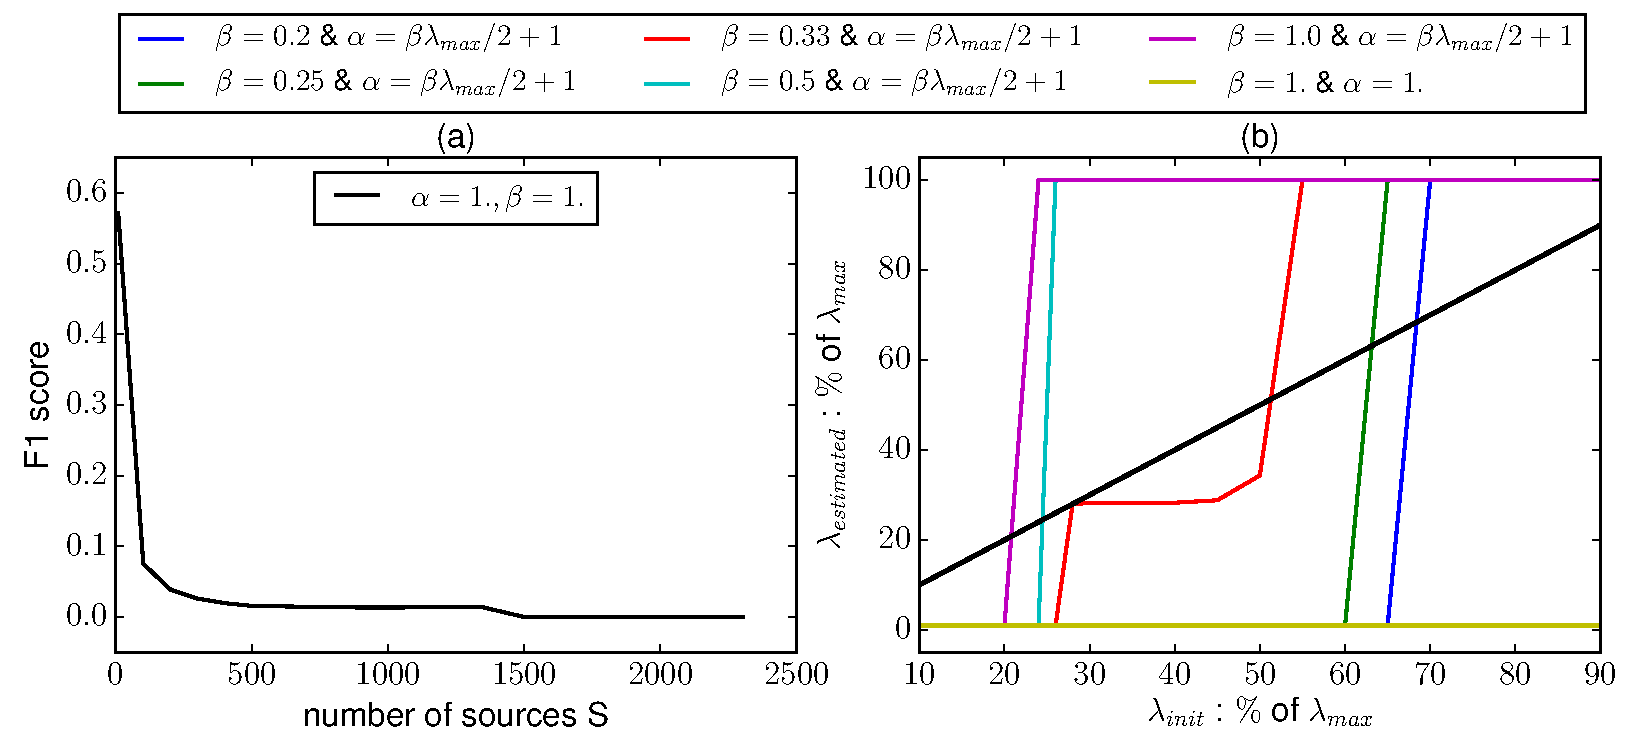
\includegraphics[width=0.95\textwidth]{hyperparam_estim/fig1_eusipco_data_size_and_fix_points_a_b}
    \caption{(a) Source identification results for different number of sources measured with F1 score using $\alpha=1$ and $\beta=1$. The higher the number of regressors the worse is the performance. (b) Estimated $\lambda$ as a function of $\lambda_{init}$ for different values of $a$ and $b$. The red curve for $\beta=0.33$ gives the best plateau, which demonstrates that $(a,b)$ shall be carefully adjusted.
    }
    \label{fig:fig1}
\end{figure}

In order to illustrate the issue when using a synthesis prior for large problems, we run the estimation of the hyperparameter $\lambda$ as suggested in~\cite{Figueiredo} using the $0.5$-homogeneous non-convex prior. Figure~\ref{fig:fig1}-(a) shows the F1 score of the source reconstruction (1 for good reconstruction and 0 for bad). The source estimation is failing for almost all the range of data size. Figure~\ref{fig:fig1}-(b) shows the results after reformulating the problem with different settings of $\alpha$ and $\beta$. One can notice that a setting as in~\cite{Figueiredo} with $\alpha=1$ and $\beta=1$ always gives an estimated $\lambda$ around $1\%$ of $\lambda_{max}$ which is not promoting the sparsity we are looking for in this kind of setting. For this aim, we varied the values of $\beta$ and computed $\alpha$ as defined before. Figure~\ref{fig:fig1}-(b) shows that for most values of $\beta$ we have rather a too low estimation of $\lambda\approx 1\%$ or a too high $\lambda\geq 100\%$ resulting in zero source found active. Interestingly setting $\beta=1/3$ gives a plateau at $\hat{\lambda}$ close to $0.3\lambda_{max}$. This is evidence of a clear fixed point for the iterative process $\lambda^{(t+1)}=f(\lambda^{(t)})$, where $f$ is the update rule of $\lambda$ in Equation~\eqref{eq4}. We use $\beta=1/3$ from now on and its corresponding $\alpha$.

Figure~\ref{fig:mxne_vs_irmxne} represents the simulated sources with stars and the estimated ones with plain lines. Figure~\ref{fig:mxne_vs_irmxne}-(a)-(b) display results with the $\ell_{2,1}$ and $\ell_{2,0.5}$ norms respectively, using one hyperparameter initialized to $\lambda=0.5\lambda_{max}$. One can see that in Figure~\ref{fig:mxne_vs_irmxne}-(a), the $\ell_{2,1}$ norm recovers the four sources with an amplitude bias (the estimated amplitude is lower than the exact one), and that several sources shown in light green are almost flat around zero but still found as active sources. There is no way to reduce the support without losing one of the four simulated sources, \textit{i.e.} the $\ell_{2,1}$ norm with one hyperparameter fails to recover the exact simulated sources.\\
The $\ell_{2,0.5}$ norm in (b) estimates the exact four source amplitudes without amplitude bias thanks to the non-convexity~\cite{irMxNE}. On the other hand, Figure~\ref{fig:mxne_vs_irmxne}-(c) shows the results for the convex penalty using one hyperparameter per source. It can be seen that it is qualitatively equivalent to the non-convex penalty. \\

The advantage of having one hyperparameter per source is to pick up only the sources involved in the measurement $\mathbf{M}$ and drop the extra almost-zero sources visible in Figure~\ref{fig:mxne_vs_irmxne}-(a) (light green). This extension produces sparser results and less amplitude bias without casting the problem as non-convex. % MAP formulation.

\begin{figure}
	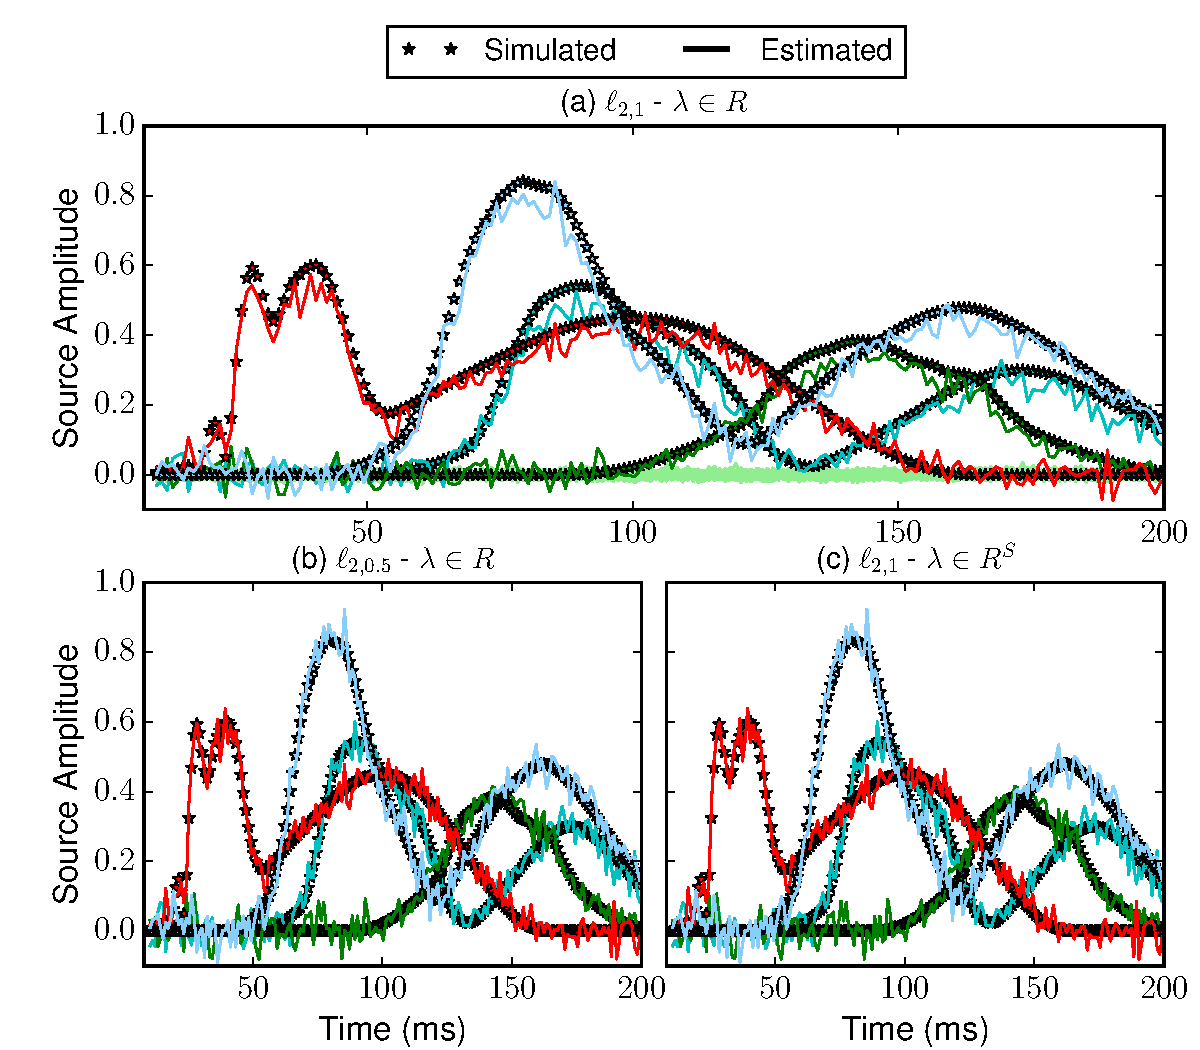
\includegraphics[width=0.95\textwidth]{hyperparam_estim/mxne_vs_irmxne}
    \caption{Source reconstruction on simulated data. (a): Source estimates obtained using $\ell_{2,1}$ with one $\lambda$. The solution is not sparse enough (the zero-sources in light green) and there is an amplitude bias between the exact amplitudes (stars) and the estimated ones (raw lines). (b): Good reconstruction of the four sources using $\ell_{2,0.5}$ and one $\lambda$, which is equivalent to the reconstruction using the $\ell_{2,1}$ norm with $\lambda\in\RR^S$ (c). Each of the four sources is encoded with a color.
    }
    \label{fig:mxne_vs_irmxne}
\end{figure}

\subsection{Experimental results with MEG auditory data}

We applied the estimation of a single hyperparameter and a hyperparameter per source using the convex $\ell_{2,1}$ penalty on a real open dataset (MNE sample dataset~\cite{MNE}). It corresponds to a dataset with $N=305$ sensors, $T=55$ time samples and $S=7498$ sources. 
Figure~\ref{fig:sample_data} shows the source amplitudes of the two auditory sources and their positions in the brain when estimating a hyperparameter per source. When using a single hyperparameter on the convex norm $\ell_{2,1}$, multiple spurious sources are found as active which replicates the simulation on Figure~\ref{fig:mxne_vs_irmxne}-(a). These source estimates in Figure~\ref{fig:sample_data} correspond to the M100 peak (peak around 100 ms) generated in the vicinity of the bilateral auditory cortices in superior temporal gyri (the relevant auditory area).

\begin{figure}
%\begin{center}	
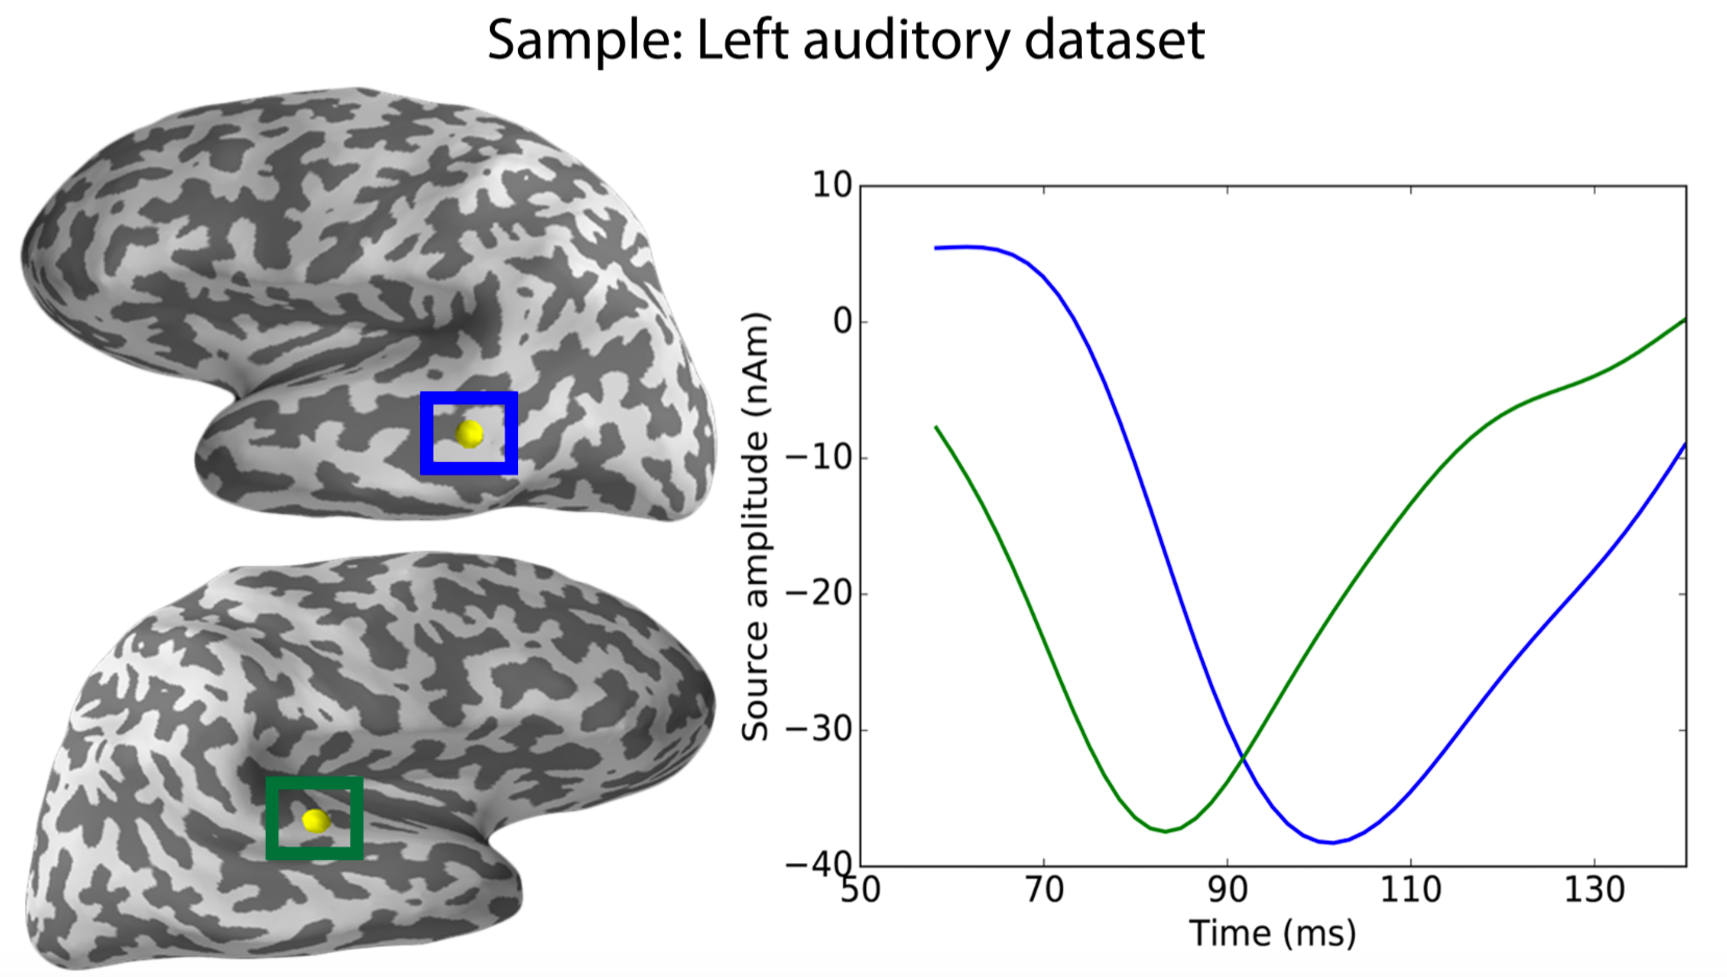
\includegraphics[width=0.95\textwidth]{hyperparam_estim/fig_sample}
    \caption{Source reconstruction on MEG auditory data (sample dataset \cite{MNE}). Source amplitude of two sources (blue and green) in the right and their corresponding positions in the brain on the left. 
    }
%\end{center}
    \label{fig:sample_data}
\end{figure}


%----------------HBM Optim------------------------------------------------------------------
\section{HBM optimization in the Bayesian formulation}
\label{section:hbm_optim}
%%%%%%%%%%%%%%%%%%%%%%%%%%%%%%%%%%%%%%%%%%%%%%%%%%%%%%%%%%%%%%%%%%%%%%%%%%%%%%%

The optimization problem defined in Equation~\eqref{eq:AO-X} reduces to an $\ell_{2,p}$-norm regularized regression problem that can be solved as described in Section~\ref{section:MM}. For solving Equation~\eqref{eq:AO-gamma}, we compute the first order optimality condition for each $i$:
\begin{eqnarray}
\label{eq:OptiGamma}
\qquad - \frac{\fronorm{\bfX^{(k)}[i]}^p}{\mathbf{\gamma}[i]^2} + \frac{1}{\beta} - \frac{( \alpha - 1 - \frac{OT}{p})}{\mathbf{\gamma}[i]} &= 0 \enspace,\label{eq:OptiGammaFirst}% \\
\end{eqnarray}

For $\alpha \geqslant O T/p + 1$, the problem in Equation~\eqref{eq:AO-gamma} is convex, and the positive root of Equation~\eqref{eq:OptiGammaFirst} is given by:

\begin{equation}
\mathbf{\gamma}[i] = \beta \left( \nu + \sqrt{ \nu^2 + \frac{\fronorm{\bfX^{(k)}[i]}^p}{\beta}} \right), \qquad \nu \mydef \frac{\alpha - 1 - OT/p}{2} \enspace.
\end{equation}

Note that similar rules to update the noise level were considered in the Bayesian Lasso~\cite{Park_Casella08,Kyung_Gill_Ghosh_Casella10} and the Scaled Lasso (see for instance~\cite{Stadler_Buhlmann_vandeGeer10,Dalalyan12}). A difference though is that the update we perform here is on the penalty term, whereas in the mentioned references, it was rather performed on the data-fitting term.

If we furthermore choose $\alpha = O T/p + 1$, then $\nu = 0$ and most terms disappear; Equation~\eqref{eq:AO-X} and~\eqref{eq:AO-gamma} hence read:
\begin{eqnarray}
\bfX^{(k)} &= \argmin_{\bfX\in\R^{SO \times T}} \left\lbrace \frac{1}{2} \fronormsq{\bfM -\bfG \bfX} + \sum_{i=1}^S \frac{\fronorm{\bfX[i]}^p}{\mathbf{\gamma}^{(k-1)}[i]} \right\rbrace \enspace, \label{eq:AO-nu0-X}\\
\mathbf{\gamma}^{(k)}[i] &= \sqrt{\beta} \sqrt{\fronorm{\bfX^{(k)}[i]}^p} \, , \quad \forall i=1,\ldots,S \enspace, \label{eq:AO-nu0-gamma}
\end{eqnarray}

which can be combined to the fixed point iteration:
\begin{equation} \label{eq:AO-nu0-2}
\bfX^{(k)} = \argmin_{\bfX\in\RR^{SO \times T}} \left\lbrace \frac{1}{2} \fronormsq{\bfM -\bfG \bfX} + \frac{2}{\sqrt{\beta}} \sum_{i=1}^S  \frac{\fronorm{\bfX[i]}^p}{2 \sqrt{\fronorm{\bfX^{(k-1)}[i]}^p}} \right\rbrace \enspace .
\end{equation}
If we compare Equation~\eqref{eq:AO-nu0-2} with Equation~\eqref{eq:MM}, we see that we re-derived the MM algorithm for $p=1$ as an alternating optimization scheme to compute the \emph{full-MAP} estimate for a specific HBM, namely using a conditional $\ell_{2,1}$ group prior and a Gamma hyper-prior with $\alpha = OT + 1$ and $\beta = 4/\lambda^2$. Using $\bfw^{(0)}[i] := 1$ in the MM scheme corresponds to starting with $\mathbf{\gamma}[i]^{(0)} := 1/\lambda =  2/\sqrt{\beta}$.\\

From previous work~\cite{strohmeier-etal:16} we know that due to the non-convexity, a good initialization of the weights $\bfw^{(0)}[i]$ in the MM algorithm is crucial for its performance, but aside uniform initialization, only heuristic initialization strategies were used, \textit{e.g.} using the same re-weighting as in the sLORETA method~\cite{Pa02}. In this thesis, we leverage the re-interpretation of the MM algorithm through the HBM framework to obtain multiple initializations in a systematic fashion, namely as samples drawn from the full posterior. This way, we can not only reach better local minima but more importantly, we can identify and characterize multiple possible sparse solutions. Such plausible solutions to the sparse regression problem in Equation~\eqref{eq:FwdEq} are the modes of the posterior distribution (Equation~\eqref{eq:full-post}) with different relative probability masses.

%----------------Sampling-------------------------------------------------------------------
\section{Posterior Sampling}
\label{section:hbm_sampling}
%%%%%%%%%%%%%%%%%%%%%%%%%%%%%%%%%%%%%%%%%%%%%%%%%%%%%%%%%%%%%%%%%%%%%%%%%%%%%%%

As outlined in Equation~\eqref{eq:AS-X} and~\eqref{eq:AS-gamma} in Section~\ref{section:HBM}, we sample the full posterior $\hipost$ by blocked Gibbs sampling, \ie we alternate between sampling the conditional distributions $p_{post}(\bfX|\bfM,\mathbf{\gamma}^{(k-1)})$ and $p_{post}(\mathbf{\gamma}|\bfM,\bfX^{(k)})$. The conditional $p_{post}(\bfX|\bfM,\mathbf{\gamma}^{(k-1)})$ is a high dimensional distribution composed of a Gaussian likelihood and an $\ell_{2,p}$ prior, where our main interest here is $p = 1$. It was demonstrated in~\cite{Lu12} that \termabb{single component Gibbs sampling}{SC Gibbs} is an efficient MCMC technique to sample such distributions. For the specific $\ell_{2,p}$ priors used here, \emph{slice sampling} can be used to perform the sub-steps in SC Gibbs sampling, namely the sampling of the one-dimensional single-component conditional densities. The resulting \emph{Slice-Within-Gibbs} sampler was examined in~\cite{Lu16}. For completeness, the details of the implementation are given in~\ref{sec:DetailsGammaSampler}.\\

The conditional $p_{post}(\mathbf{\gamma}|\bfM,\bfX^{(k)})$ factorizes over groups $i$:
\begin{equation}
\fl \qquad p_{post}(\mathbf{\gamma}[i]|\bfM,\bfX^{(k)}) \propto \exp \left( -\frac{\fronorm{\bfX^{(k)}[i]}^p}{\mathbf{\gamma}[i]} - \frac{\mathbf{\gamma}[i]}{\beta} + (\alpha - 1 - O T/p) \log(\mathbf{\gamma}[i]) \right) \enspace. \label{eq:conPostGammai}
\end{equation}
For the case of $\alpha = O T/p + 1$, which is our main interest due to its connection to MM revealed in the previous section, Equation~\eqref{eq:conPostGammai} reduces to:
\begin{equation}
\fl \qquad p_{post}(\mathbf{\gamma}[i] |\bfM, \bfX^{(k)}) \propto \exp \left(- \frac{\fronorm{\bfX^{(k)}[i]}^p}{\mathbf{\gamma}[i]} \right) \exp \left(- \frac{\mathbf{\gamma}[i]}{\beta} \right) \enspace, \label{eq:conPostGammaiRed}
\end{equation}
which can be sampled with a simple accept-reject algorithm as described in Section~\ref{sec:DetailsGammaSampler}. The complete procedure is described in Algorithm~\ref{alg:sampling}. Therein, $K_0$ refers to the burn-in size, \ie the initial samples that are discarded, $K$ to the sample size of the blocked Gibbs sampler and $K_{SC}, K_{SS}$ to the sample sizes of the SC Gibbs and the slice sampler that carry out the sampling in the sub-steps.

{\fontsize{4}{4}\selectfont
%above is to make smaller fonts in algorithm
\begin{algorithm}[t]
\SetKwInOut{Input}{input}
\SetKwInOut{Init}{init}
\SetKwInOut{Parameter}{param}
\caption{\textsc{Block Gibbs Sampling scheme}}
\Input{$\bfM, \bfG $, $\bfX^{(-K_0)}$, $\mathbf{\gamma}^{(-K_0)}$, $K_0$, $K$, $K_{SC}$, $K_{SS}$, $\alpha$, $\beta$}
% \Parameter{}

\For{
        $k = -K_0+1$ to $K$
    }
    {%Sample $(\bfX,\gamma) \sim p_{post}(\bfX,\gamma |\bfM)$ via \textbf{Block Gibbs:}
    Set $\bfX^{(k)} = \bfX^{(k-1)}$.\\
    \For{
    		$k_{SC} = 1$ to $K_{SC}$
    		}
    		{
    		Draw a random permutation $P$ of $\{1,\ldots,S\}$\\
    		\For{
    			$l \in P$
    			}
    			{
			Sample $\bfX^{(k)}[i,j] \sim p_{post}(\bfX[i,j]|\bfX^{(k-1)}[-(i,j)],\bfM,\mathbf{\gamma}^{(k)})$, $\forall (i,j)\in [l]$ - via $K_{SS}$ steps of \textbf{Slice Sampling} Algorithm~\ref{alg:slicesampler}.
			}
		}
	{Sample $\gamma^{(k)}_{i} \sim p_{post}(\gamma_{i}|\bfM,\bfX^{(k)})$, $\forall i =1,\ldots,n$ via \textbf{Accept-Reject} Algorithm~\ref{alg:acceptreject}.}

    }
\Return{$\{\bfX^{(k)},\mathbf{\gamma}^{(k)}\}_{k=1}^K$}
\label{alg:sampling}
\end{algorithm}
}

%----------------uncertainty maps-----------------------------------------------------------
\section{Study of the different modes defining uncertainty maps of inverse problems}

%----------------Experiments-----------------------------------------------------------
\section{Experiments}
We now examine the benefits of our re-interpretation of the MM algorithm described in Section~\ref{section:MM} as a specific way to compute a full-MAP estimate for a specific HBM as described in Sections~\ref{section:HBM} and ~\ref{section:MM}.
In particular, we investigate how using MCMC sampling of the posterior distribution as described in Section~\ref{sub:sampling} can help getting better initializations for the optimization algorithm.
We first present results for a simulated MEG dataset and then for two experimental MEG/EEG datasets.

\subsection{Simulation study}
We generated a realistic simulation based on a free-orientation ($d=3$) source model with $n=7498$ cortical locations and $m=306$ MEG sensors. Two of these locations were selected to be active, one in each hemisphere. One of the sources had a deep ventral location in the inferior occipital gyrus (Figure~\ref{fig:simulated_data}-c), and the second one had a more superficial location in the motor cortex (Figure~\ref{fig:simulated_data}-a). Their corresponding waveforms are shown in Figure~\ref{fig:simulated_data}-b. When passed to the solvers, they are cropped between 40 to 180 ms to keep only the two peaks. This leads to $t=43$ time samples.

\begin{figure}[htp]
	\centering
	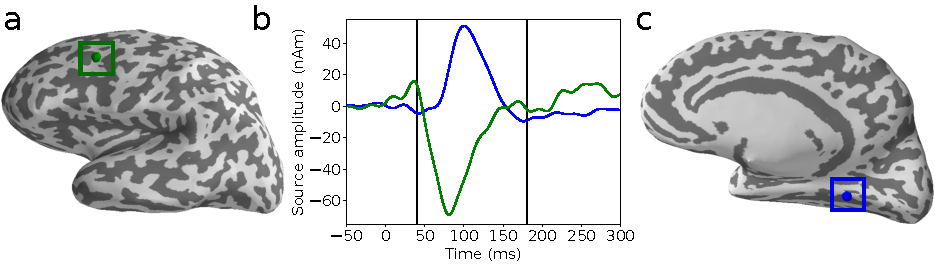
\includegraphics[clip,width=.9\columnwidth]{hbm/simulated_data}%

	\caption{Simulated MEG dataset. a) and c) show superficial and deep source (hidden in the medial view) locations, respectively. b) gives their corresponding waveforms color-coded by location.}
	\label{fig:simulated_data}
\end{figure}

The aim of the simulation is to answer two separate questions. First, we want to know whether we are able to find better source estimates using MCMC-derived initializations than with the uniformly initialized MM Algorithm~\ref{alg:adpative_lasso}.
For this, we first run the MM Algorithm~\ref{alg:adpative_lasso} using a uniform initialization, \ie $\bfw^{(0)}_{i} = 1, \forall i=1\in [1,\cdots,S]$, with $\lambda = 0.05\lambda_{max}$ where $\lambda_{max}= \max_{1 \leq i \leq S} \fronormsq{(G^\top M)[i]}$ is the smallest regularization value for which no source is found as active using an $\ell_{2,1}$ regularization~\cite{Ndiaye_Fercoq_Gramfort_Salmon15,strohmeier-etal:16}. As described above, this corresponds to computing a full-MAP estimate for the HBM with $p=1$, $\alpha = OT +1 $, $\beta = 4/\lambda^2$ using the alternation scheme \label{eq:AO-nu0-X} initialized with $\mathbf{\gamma}^{(0)}[i] = 1/\lambda, \forall i=1\in [1, \cdots, S]$.

Then, we sampled the corresponding posterior distribution given in Equation~\eqref{eq:full-post} using Algorithm~\ref{alg:sampling} with $K_0 = 300$, $K = 900$, $K_{SC} = K_{SS} = 1$. From each $\mathbf{\gamma}^{(k)}$ of the $K = 900$ obtained $\mathbf{\gamma}$ samples, we construct an initialization $\bfW^{(0)}$ for the MM Algorithm~\ref{alg:adpative_lasso} by setting $\bfw^{(0)}[i] = \lambda \mathbf{\gamma}^{(k)}[i], \forall i=[1,\dots,S]$. Figure~\ref{fig:simu_MM_best_MCMC}-c shows the histogram of the objective function values (computed with Equation~\ref{eq:lasso_new_gram}) obtained this way. The vertical black bar shows the value of the objective function of the uniformly initialized MM solver and we can see that some initialization indeed lead to source estimates with a lower objective value. Figure~\ref{fig:simu_MM_best_MCMC}-a and Figure~\ref{fig:simu_MM_best_MCMC}-b show the locations of the estimated sources resulting from uniform and best MCMC-based initialization. For the artificial source in Fig.~\ref{fig:simu_MM_best_MCMC}-a, both results find the exact location, so they are superposed. For the deeper source in Figure~\ref{fig:simu_MM_best_MCMC}-b, neither result finds the exact position, but the MCMC-based initialization is closer. This means that the result did not only improve from an optimization point of view, but also judged by the quality criteria of the given application.

\begin{figure}[htp]
	\centering
	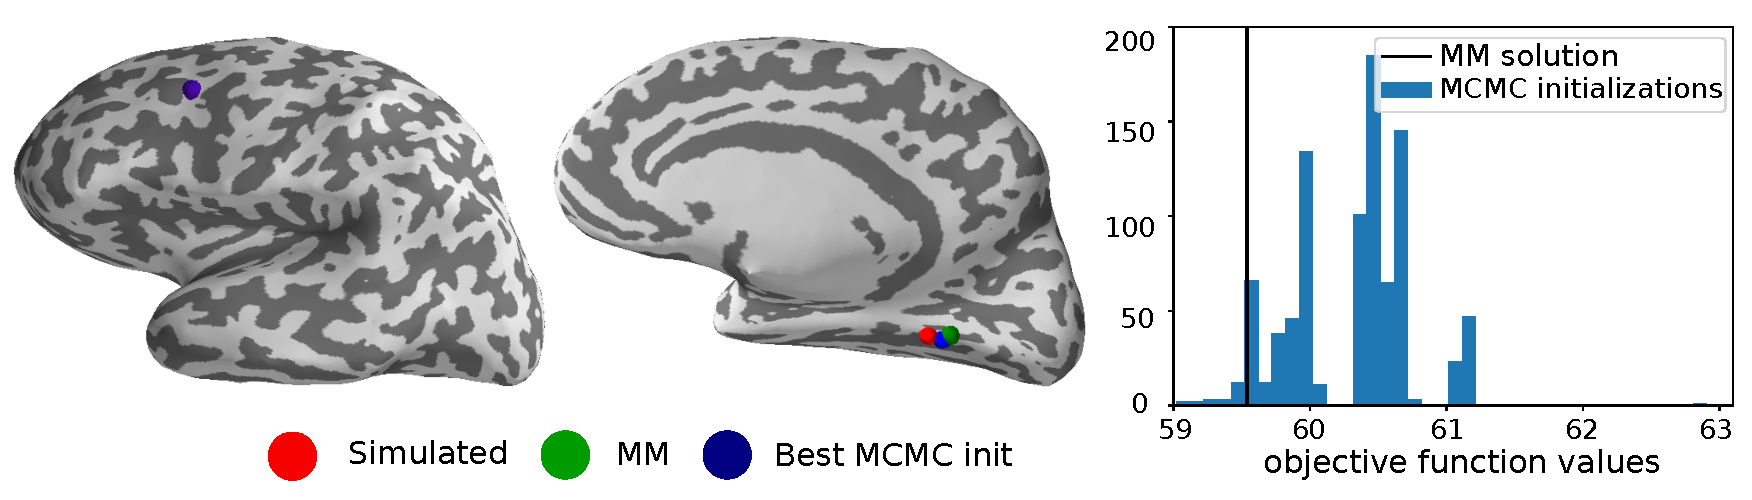
\includegraphics[width=\columnwidth]{hbm/simulated_data_hist_vertices}
	\caption{Location of simulated and estimated sources using the uniformly initialized MM solver (denoted as ``MM'') and best MCMC-based initialization in terms of objective function value. Left: estimation of the artificial source on the left hemisphere. Middle: estimation of the deep source on the right hemisphere. Right: histogram of the objective function value for 900 MCMC initializations. The uniform initialization used for the MM (black vertical line) is not very bad, meaning that the basic MM is able to recover a good source estimates for some configurations. See Figure~\ref{fig:hist_real_datasets} for a case where the basic MM fails.}
	\label{fig:simu_MM_best_MCMC}
\end{figure}

Finding the correct support in a sparse under-determined regression problem like Equation~\eqref{eq:FwdEq} is inherently of combinatorial complexity. In our two approaches, this is reflected in the non-convexity of the objective function (Equation~\eqref{eq:L2pReg}) and the multi-modality of the joint posterior distribution (Equation~\eqref{eq:full-post}), respectively. The second question we want to investigate is whether the methods we developed here can reveal or quantify some of the ambiguity and uncertainty of this sparse support identification problem. Traditional uncertainty quantification (UQ) measures such as variance estimates of $\bfX$ or $\mathbf{\gamma}$ fail to do so as they cannot capture the multi-modality of the posterior in a satisfactory way. In addition, no sample $\bfX^{(k)}$ is exactly sparse: as the posterior distribution is a continuous probability density, the probability of event $\{\bfX^{(k)}[i] = 0\}$ is zero, which means that the whole support of $\bfX^{(k)}$ is active with probability $1$. Even a thresholded average of the support of $\bfX^{(k)}$ will only reveal the average probability of a location being part of the support. In source analysis, it is arguably more interesting which networks of sources from different brain areas have most likely produced a given data set, a question left open by these measures. Here, we propose to tackle this question in a different way.

\begin{figure}[htp]
	\centering
	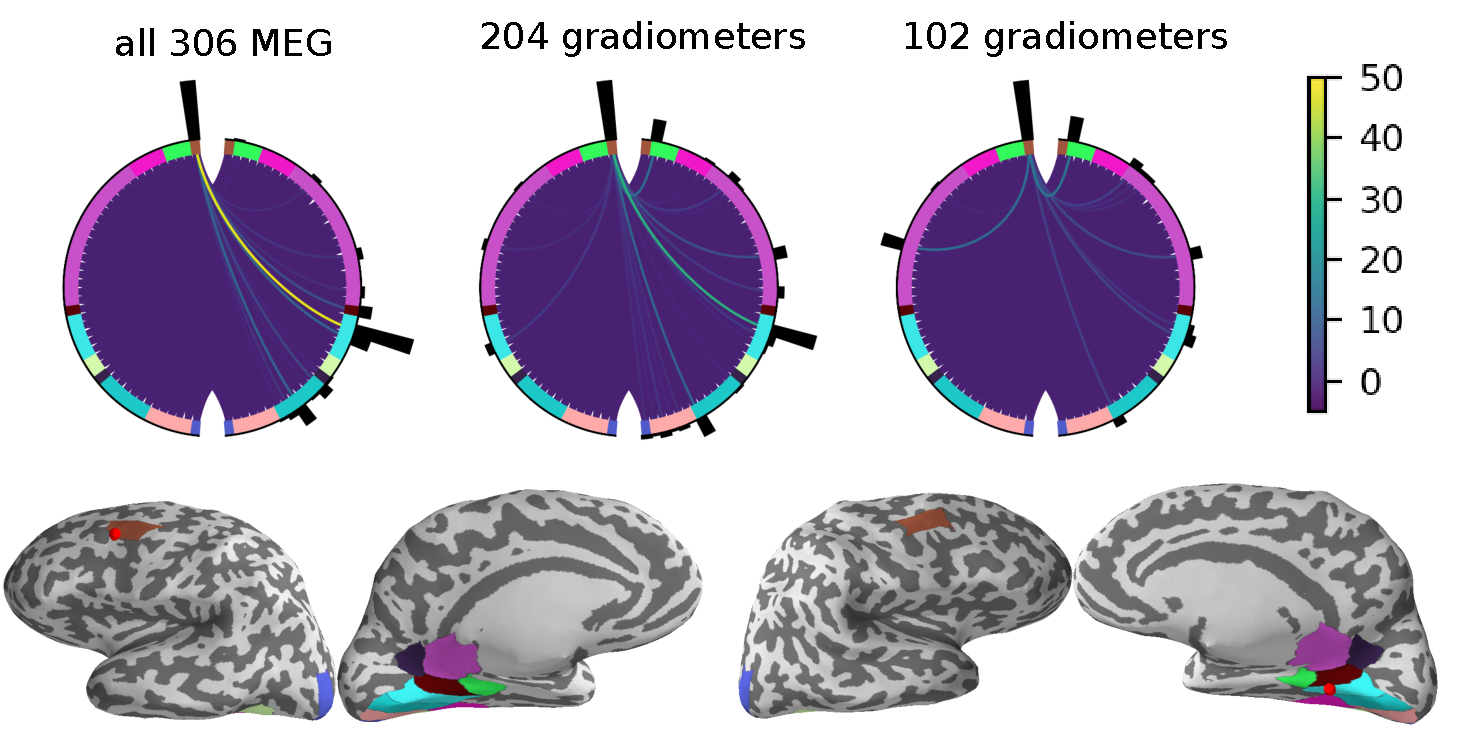
\includegraphics[clip,width=0.98\columnwidth]
{hbm/simulated_circular_plots_new}

	\caption{Source network analysis for simulated data: for a clearer presentation, the set of 900 initializations was thinned to the 100 that gave the lowest objective function (Equation~\eqref{eq:L2pReg}). The first row of sub-figures displays the support of these best local minima in the following way: each position in the circle represents a source location that was part of the support of at least one minima for one sensor configuration. The black bar attached to each position corresponds to the relative frequency with which this source location appeared as part of the support. Two positions are connected by a line if they were simultaneously part of the support and the color of this line corresponds to the relative frequency with which this happened. Note that the background of the circle is white, but densely covered by purple lines indicating rare connections. The positions are placed left or right, depending on which hemisphere they belong to. For symmetry, for each active source location, its counterpart on the other hemisphere was included in the graphic as well. In addition, the positions are grouped and colored based on a parcellation of the brain into anatomical regions (taken from an atlas). The second row of sub figures shows these regions in the brain and the simulated sources.}
	\label{fig:results_simu_circular}
\end{figure}

Our procedure of initializing an MM iteration with a sample from the posterior distribution yields different local minima of Equation~\eqref{eq:L2pReg}, \ie approximate solutions to Equation~\eqref{eq:FwdEq} that fulfill our \emph{a priori} knowledge of a sparse support, but it also yields the relative frequencies with which these minima are found by the MM algorithm. If we assume that the division of $\R^{SO\times T}$ into attractors of the MM algorithm roughly overlaps with the division of $\R^{SO\times T}$ into modes of the marginalized posterior over $\bfX$ within the HBM framework, this relative frequency corresponds to the relative volume of the local minima of Equation~\eqref{eq:L2pReg}. The latter is a better measure to compare different local minima than their depth (a local minimum that is deep but thin corresponds to an unstable source estimate). While a mathematically more profound and detailed analysis of this heuristic is left for future work, we examine here if this approach reacts to changes in the measurement design in the way we would expect. To do so, we switch from using all 306 MEG sensors to using only 204 gradiometers or each other gradiometer (102 sensors). By reducing the number of sensors we increase the under-determinedness of the problem and the intuition is that it should lead to
more variability among the plausible sparse solutions. The graphical analysis presented and described in Figure~\ref{fig:results_simu_circular} and Figure~\ref{fig:results_simu_heat_maps} confirms this. A first observation is the superficial source in the premotor cortex was correctly identified as part of the support of every local minima when using the full 306 MEG sensors. It was however sometimes miss-localized when reducing the number of sensors (Figure~\ref{fig:results_simu_circular}). A second observation is that the spatial spread of these miss-localizations is smaller for this superficial source than it is for the deep source. This deep source in the ventral cortex is more difficult to find even with all sensors. Indeed, none of the 100 best initialization perfectly localized the deep simulated source. In general, we can clearly see how the ambiguity increases when decreasing the number of sensors, and how the distribution of source networks gets more fuzzy. However, our analysis also provides useful local measures of these phenomena.


\begin{figure}[htp]
	\centering
	\begin{minipage}{\linewidth}
		\begin{minipage}{0.9\linewidth}
			\setlength\tabcolsep{0.1pt} % default value: 6pt
			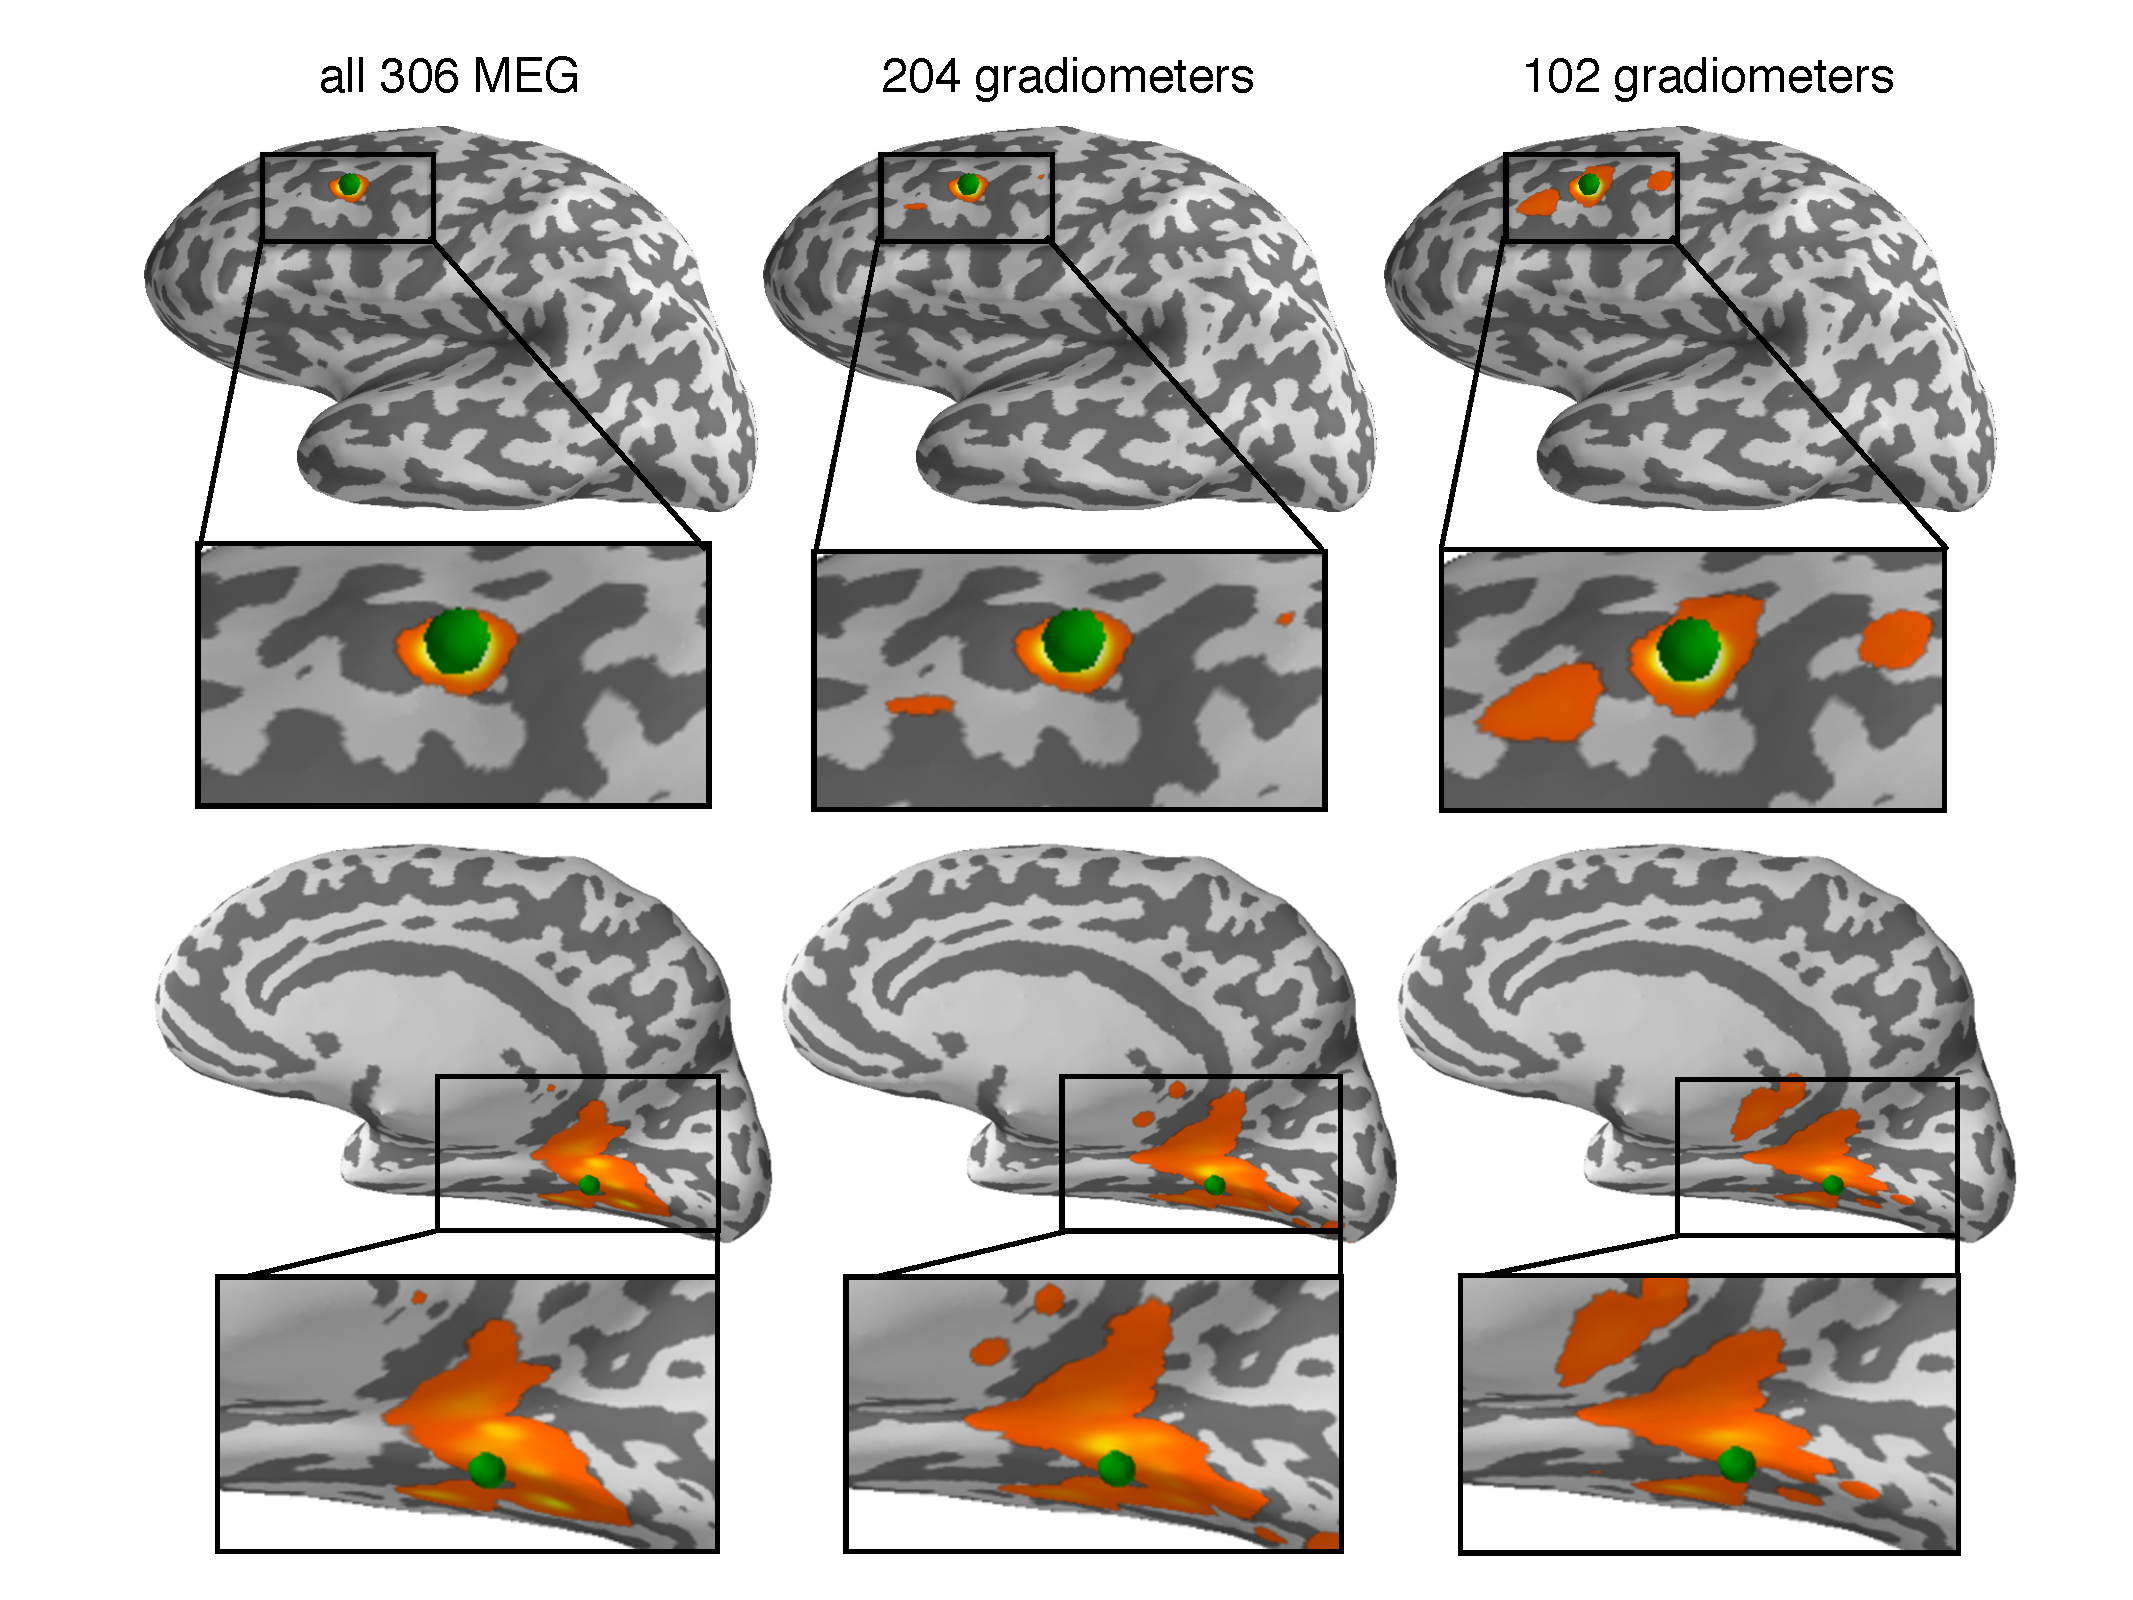
\includegraphics[width=\columnwidth]{hbm/sample_simulated_heat_maps}%
		\end{minipage}
		\begin{minipage}{0.09\linewidth}
				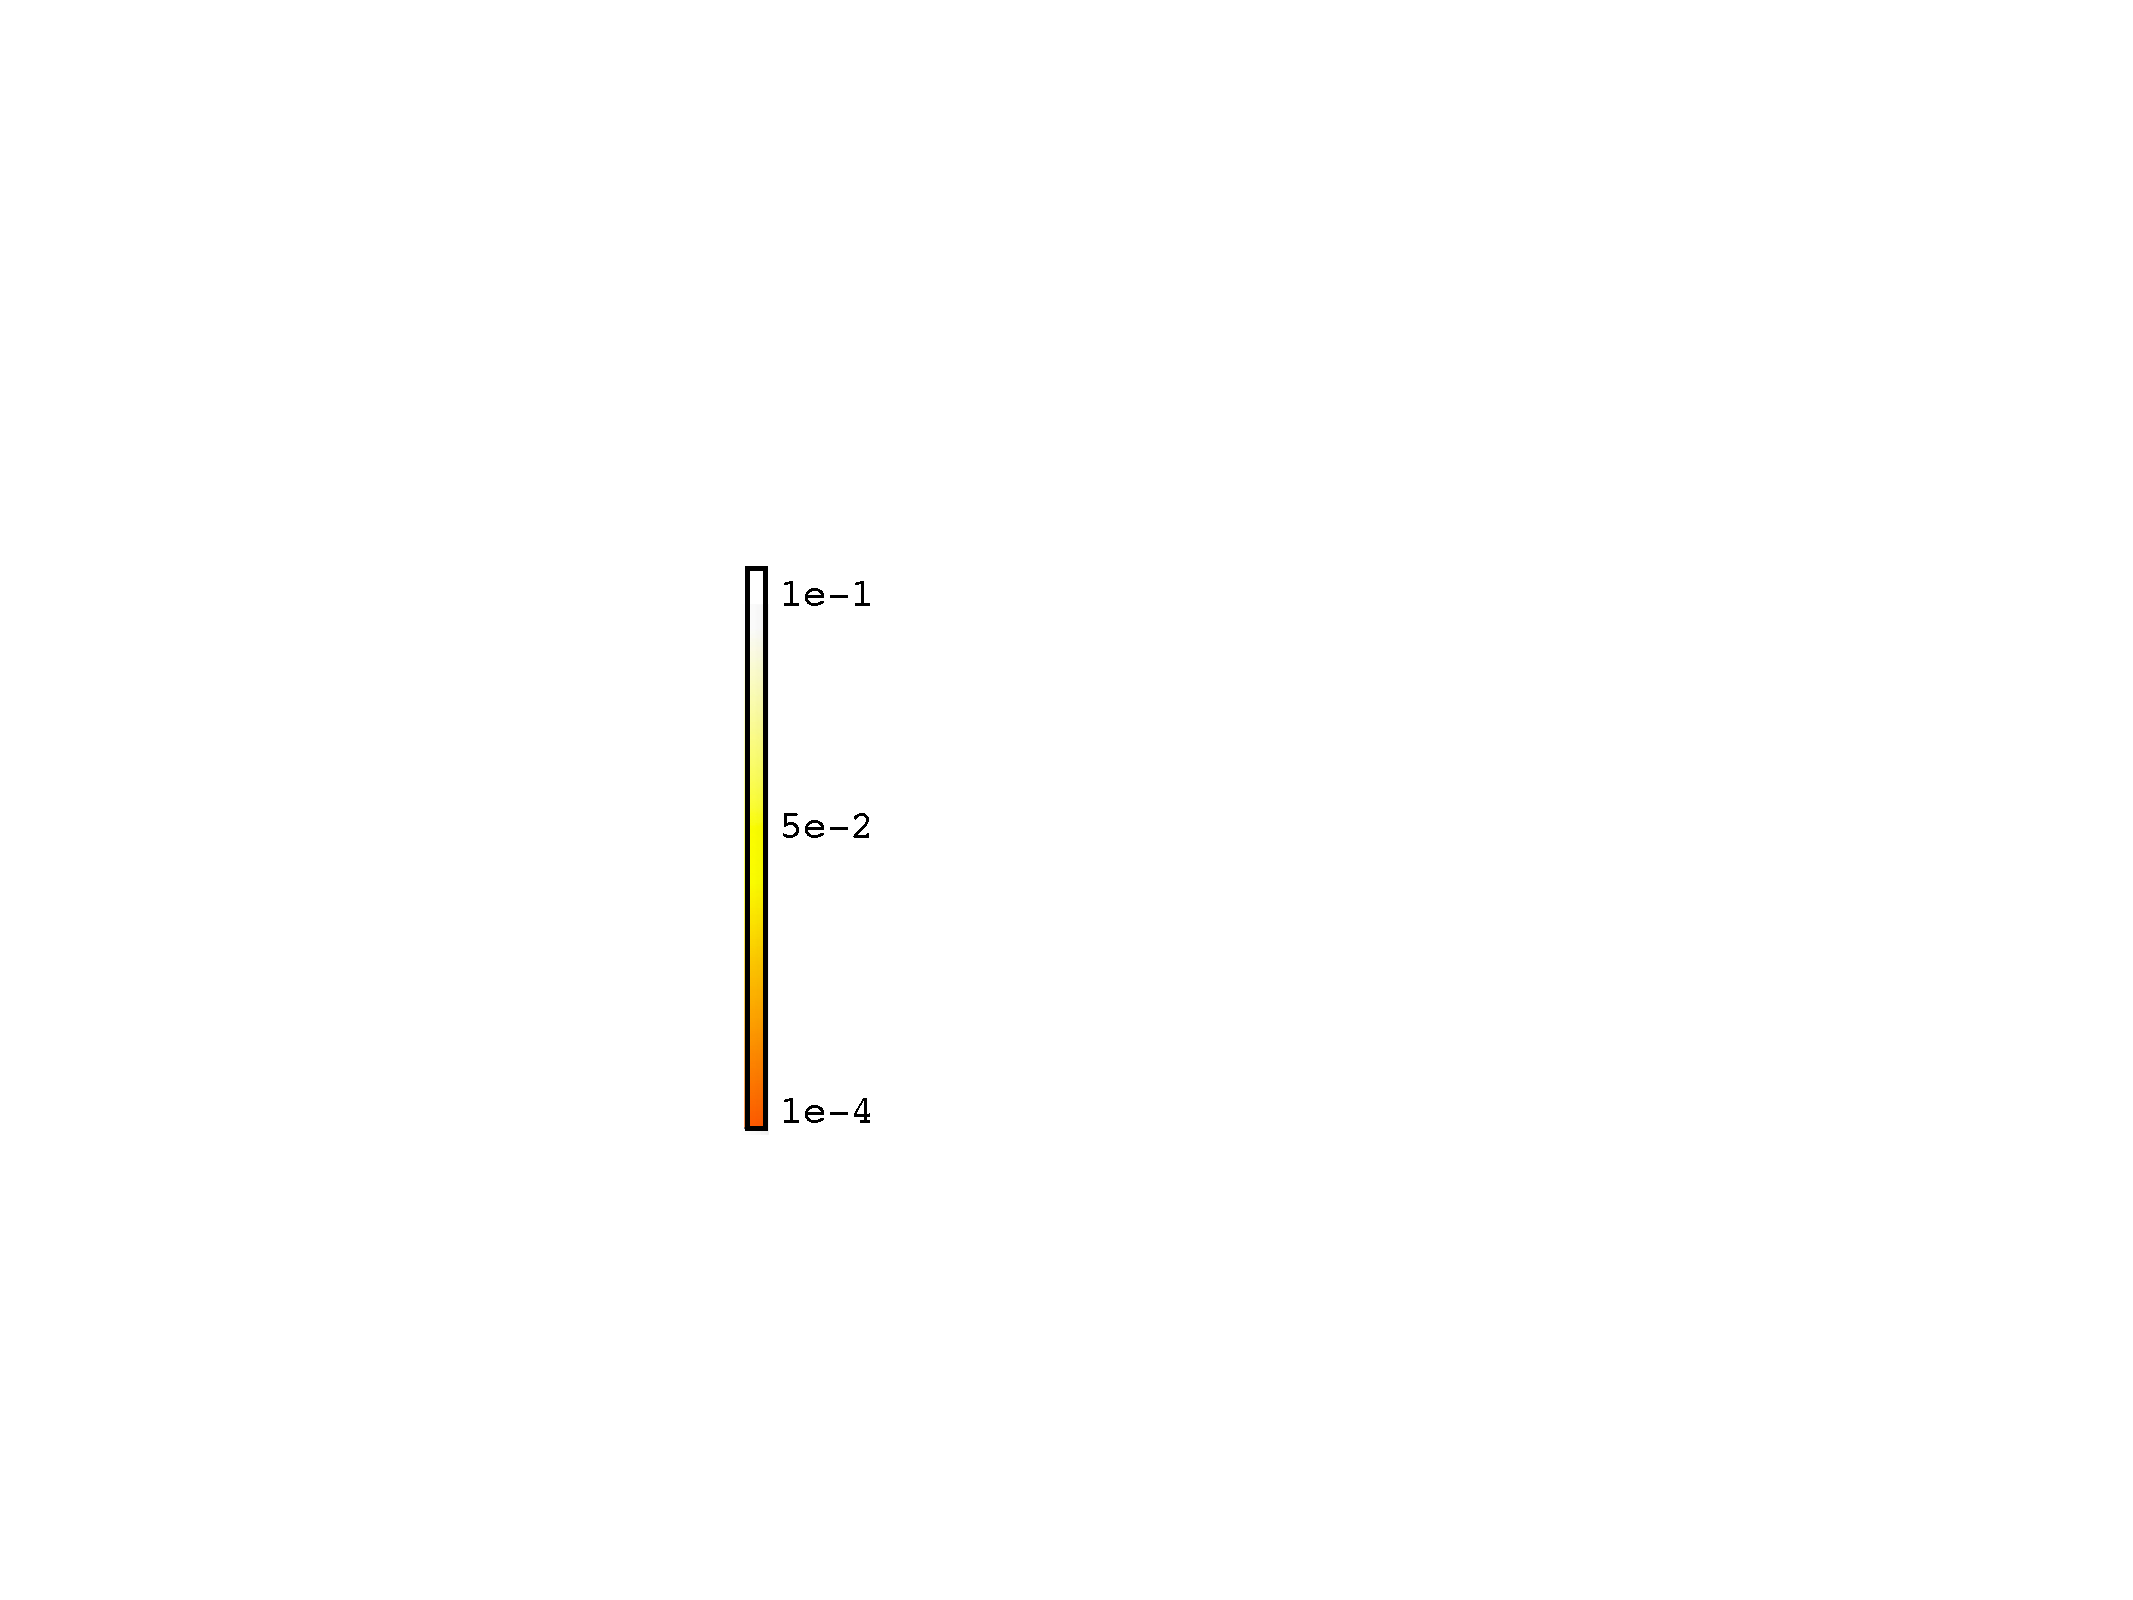
\includegraphics[width=\columnwidth]{hbm/colorbar_heat_maps_key}%
		\end{minipage}
	\end{minipage}
	\caption{The support of the MM results based upon 900 MCMC-based initializations were extracted to build an uncertainty map. The relative frequencies with which each source location was part of the support was computed and plotted on the brain surface together with the two simulated sources (green dots). Each column corresponds to the results for each of the three sensor setups examined. Less the number of sensors and/or more the source is deep, more uncertainty in the brain map.}
	\label{fig:results_simu_heat_maps}
\end{figure}


\subsection{Experimental MEG data}
We now repeat our analysis with two experimental open datasets. The first one is a recording of auditory evoked fields (MNE sample dataset~\cite{mne-python}). The second one contains visual evoked fields (visual condition of MNE sample dataset) for which source localization is a more difficult task due to the proximity between neural sources. The true nature of the underlying source network is also less clear for this second dataset.

Figure~\ref{fig:hist_real_datasets} shows the equivalent to Figure~\ref{fig:simu_MM_best_MCMC} for both datasets. Again, we see that lower objective function value can be obtained using MCMC-based initializations. The auditory sample dataset is commonly assumed to be generated by two bilateral focal sources around the auditory cortices in the superior temporal gyrus of the temporal lobe. Due to the superficial nature of these sources and their large distance, estimation of their position is regarded as a relatively simple task. Indeed, the histogram shows that using MCMC-based initializations does not help a lot to reduce the objective function compared to a uniformly initialized MM solution. In the case of the visual dataset, where several closed-by sources are active, the difference is however quite drastic. The majority of the MCMC-based initializations lead to lower values of the objective function. Looking at the source distribution plots on the brain for both datasets, one can also observe more complex source configurations for the visual data.
% XXX : say here that there is nothing on right hemi for best MCMC?

Next, we repeat the graphical source network analysis from Figure~\ref{fig:results_simu_circular} for the two datasets. Figure~\ref{fig:circular_plots_LAud} shows the results for the auditory dataset and three sensor configurations: all 364 EEG + MEG sensors, all 306 MEG sensors or each other sensor resulting in 182 EEG + MEG sensors. One can see how adding EEG to MEG sensors reduces the ambiguity of the regression problem. The plots show less but more prominent modes, \ie the posterior mass is concentrated on fewer stable source configurations. We also see that the locations of the most prominent modes shift
This is consistent with results of other studies on EEG-MEG combination \cite{MoStBrHa08,Lu14,AyVoKuHeKuGaHaWeKeRaWoHe14} as EEG is sensitive to some sources that MEG is almost blind to, \eg sources with a strong radial component. If we subsample the EEG+MEG sensors by only using every other location, the ambiguity and spatial spread of the recovered support increases. One can see that there is more activity in the dark green label, which corresponds to a brain area commonly not associated with auditory responses.% On the other hand, there is less activity in the light green label, which marks central areas of the auditory system.
%\ag{what green region do you have in mind?}\felix{Good question, that corresponded to the coloring/parcelation in the old figures. In the new ones, I can't really recall what I wanted to say. Maybe we just drop the sentence and not over-interpret our results?}
The connections between source locations show that none of the modes found really stands out, \ie is found much more often compared to the others. Most of the connections do not occur more than 200 times within the 900 samples, so they are part of the purple background of low frequency connections in the plots.\\
Figure~\ref{fig:circular_plots_LVis} shows the same results for the more complex visual dataset. Compared to the auditory dataset, we see that even with all sensors, the ambiguity of the regression problem seems to be a lot higher compared to the auditory dataset: we see that the posterior mass is distributed among many more source configurations. For the other two sensor configurations, we see similar effects as in the auditory data set. Nevertheless, it can be noticed that the large majority of identified sources with all MCMC initializations are on the right hemisphere. This is consistent with the known functional organisation of the visual cortex. Indeed, in this experimental condition the subject was presented with checker board flashes on the left visual hemifield which is known to primarily project onto the right hemisphere of the cortex.


\begin{figure}[htp]
	\centering
	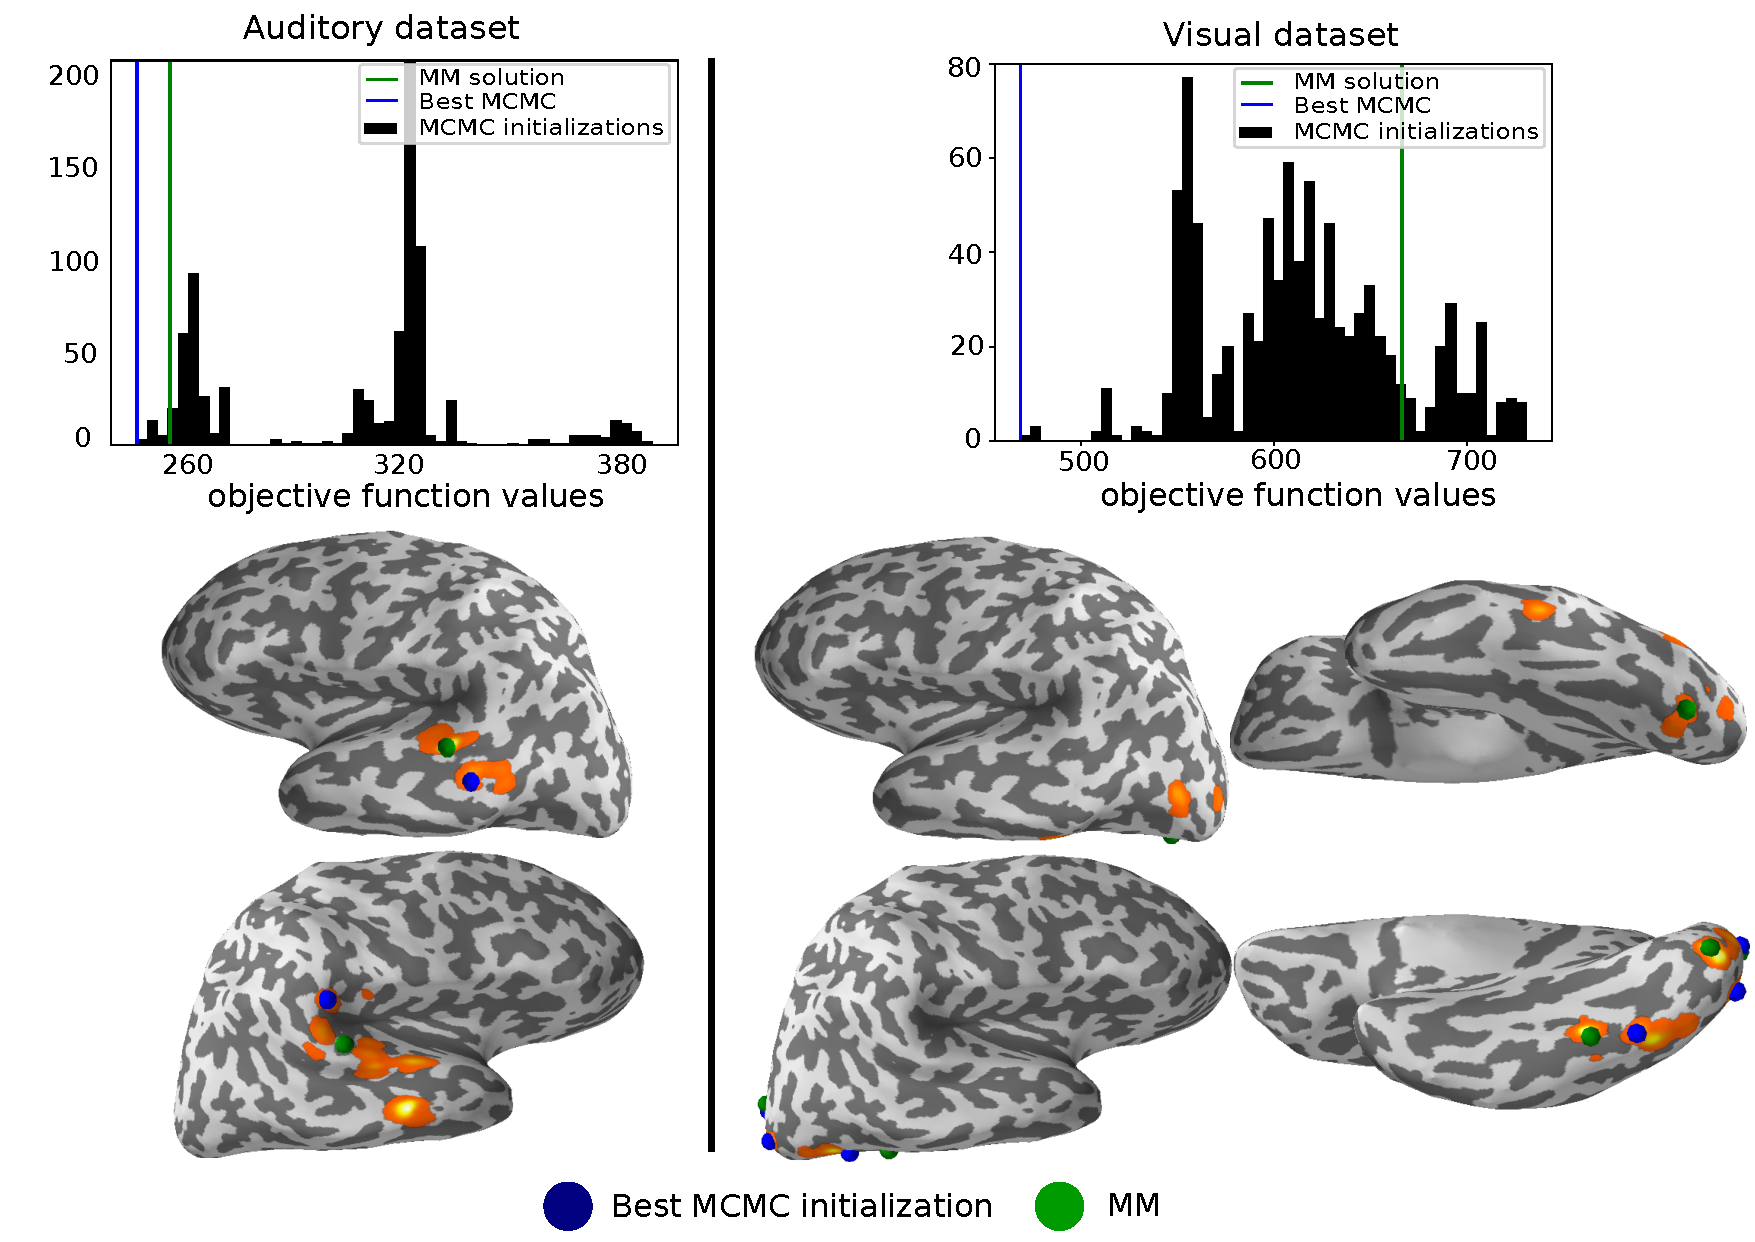
\includegraphics[width=\columnwidth]{hbm/sample_data_hist_vertices}%
	\caption{Histogram of the objective function value for 900 MCMC initializations for auditory and visual datasets (306 MEG sensors). The histogram for visual dataset shows more MCMC initializations that outperform the uniform one in the MM solution. Under each histogram, these source configurations are shown on the left and right hemisphere.
	}
	\label{fig:hist_real_datasets}
\end{figure}



\begin{figure}[htp]
	\centering
	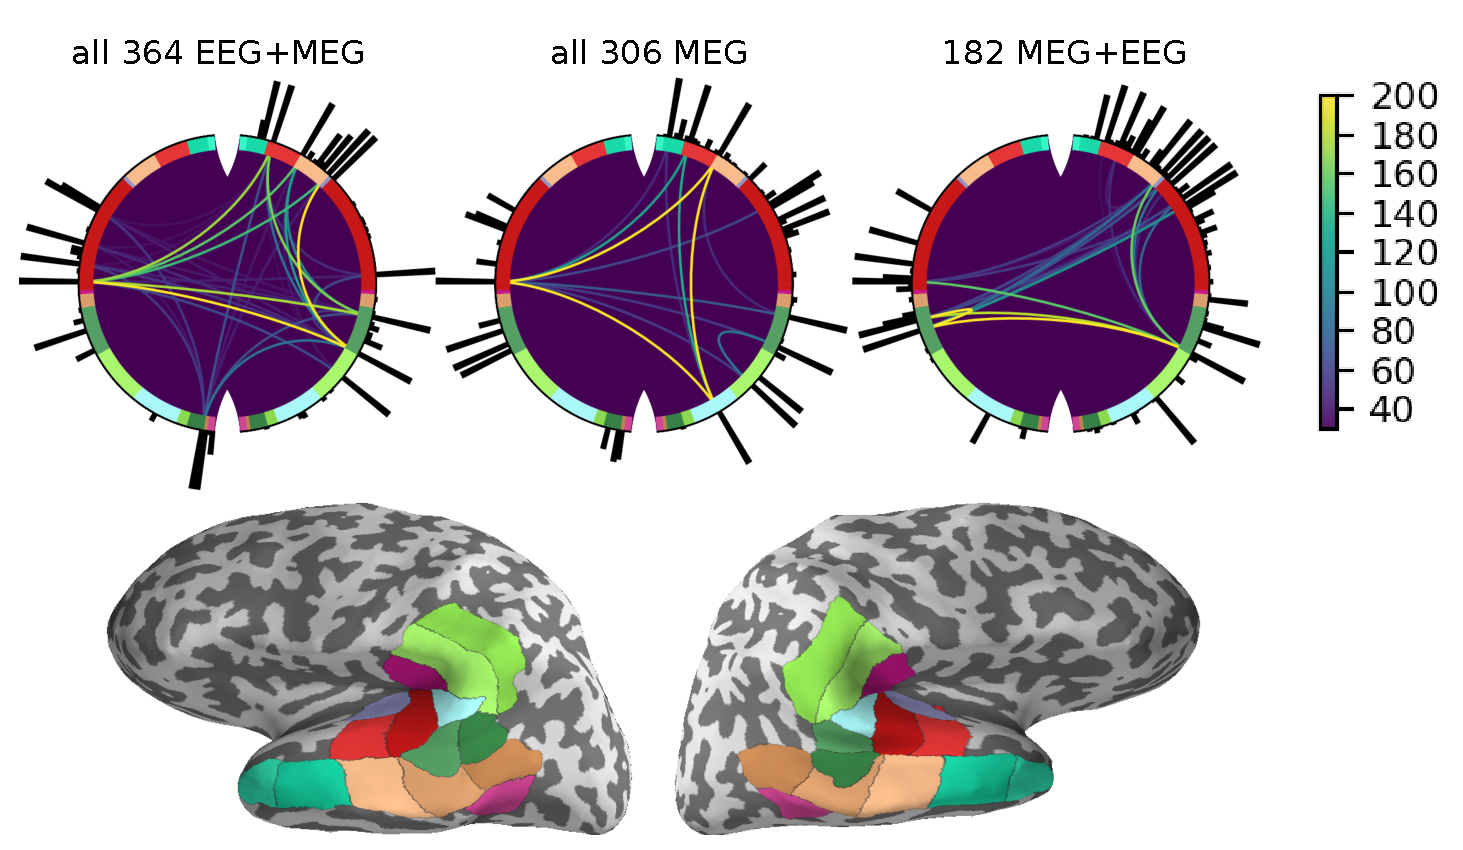
\includegraphics[width=\columnwidth]{hbm/LAud_circular_plots_new}%
	\caption{Source network analysis for auditory data. The figures are constructed in the same way as described in Figure~\ref{fig:results_simu_circular} except that all 900 MCMC initializations are displayed.}
	\label{fig:circular_plots_LAud}
\end{figure}



\begin{figure}[htp]
	\centering
	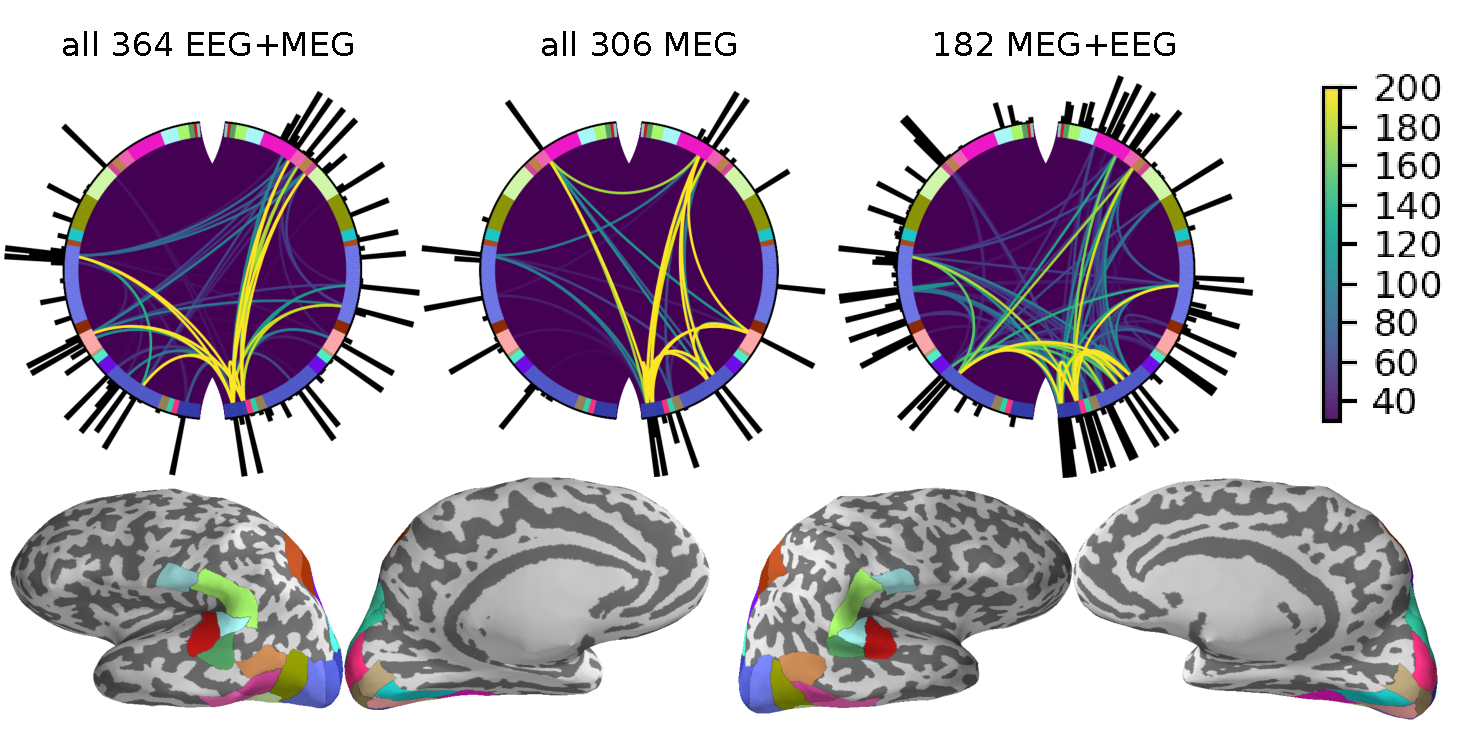
\includegraphics[width=\columnwidth]{hbm/LVis_circular_plots_new}%
	\caption{Source network analysis for visual data. The figures are constructed in the same way as described in Fig.~\ref{fig:results_simu_circular} except that all 900 MCMC initializations are displayed.}
	\label{fig:circular_plots_LVis}
\end{figure}

%----------------Conclusion-----------------------------------------------------------------
\section{Conclusion \& Perspective}
\label{sec:Dis}
%%%%%%%%%%%%%%%%%%%%%%%%%%%%%%%%%%%%%%%%%%%%%%%%%%%%%%%%%%%%%%%%%%%%%%%%%%%%%%%
%%%%%%%%%%%%%%%%%%%%%%%%%%%%%%%%%%%%%%%%%%%%%%%%%%%%%%%%%%%%%%%%%%%%%%%%%%%%%%%

Scientific literatures relying either on frequentist or on Bayesian statistical inference often coexist in many fields ranging from machine learning, inverse problems, signal processing or computational biology.
In this work, we started from an under-determined, ill-conditioned MMV / multi-task regression problem and examined two seemingly unrelated approaches - MM as an optimization technique for tackling non-convex optimization problems arising in frequentist regression, and HBM as a Bayesian prior modeling framework. We showed that one obtains the same algorithms, and therefore the same solutions, when considering some specific choices of models, parameters and inference strategies. In particular the parallel was done between the $\ell_{2,1/2}$-norm regularized regression by MM and the full-MAP estimation for $\ell_{2,1}$ hierarchical priors with specific Gamma hyper-priors. We further showed that this conceptual parallel can be exploited to improve the MM solution by providing well-informed algorithmic initializations.
% , and also to complement the single-point result given by MM - in our case a sparse neuronal source configuration - with a more statistical analysis of the multitude of plausible solutions to the non-convex regression problem.

% For this, we constructed a multi-layered Gibbs sampler for the joint posterior density of our HBM. This sampler has an efficient sub-sampler for $\ell_{2,1}$ priors at its core. We showed that the MCMC scheme is able to quickly jump between the different attractors of the MM scheme by using each sample as an initialization to the MM computation. Each MM computation can then be done with a state-of-the-art convex solver using block coordinate descent techniques and acceleration techniques based on active set strategies.

% As we end up in a different mode with almost every sample, this procedure is well suited to explore different plausible source configurations in more detail. \felix{we don't show this at the moment but it would be easy to add a plot.}
% \textcolor{red}{\textbf{Alternative paragraph:}

For this, we first constructed a multi-layered Gibbs sampler for the joint posterior density of our HBM.
Each sample is then used to initialize the MM step done with a state-of-the-art convex solver using block coordinate
descent techniques and acceleration strategies based on active sets. The sampler used has also an efficient sub-sampler for $\ell_{2,1}$ priors at its core. Despite the multi-modality of the posterior, the MCMC scheme is able to jump rapidely between the different attractors of the MM scheme. Indeed, using each sample as an initialization to the MM computation, one ends up in many different local minima (cf. Fig~\ref{fig:hist_real_datasets}, Fig~\ref{fig:circular_plots_LVis}). 
Therefore, this procedure allows us to reveal and explore different plausible source configurations in more details.
% }
% 

Based on this observation, we showcased how one can use the chain of local minima found by MCMC-initialized MM to analyze the variability of the different sparse solutions. Note that this is different from traditional and generic Bayesian uncertainty quantification techniques that use for example covariance estimates or credible sets derived from posterior samples~\cite{szabo2015frequentist}. It is also different from methods developed specifically for parametric M/EEG source localization based on dipole fitting~\cite{Fuchs20041442,Darvas2005355}. These latter approaches cannot easily be transferred to sparse, non-parametric approaches. Using our developed techniques on simulations and actual data, one could observe that uncertainty in MEG/EEG is location specific and also source configuration specific. This is of course well-known by experts in this field, but here we provide a computational approach to visualize it and quantify it.
This is an important incentive to develop such automated, data-dependent methods to quantify uncertainties in the context of MEG/EEG source imaging. In more conventional imaging methods such as computer tomography (CT) or magnetic resonance imaging (MRI), the signal originates from weak tissue interaction with strong external fields and the forward operator $\bfG$ depends almost exclusively on the physical properties of the scanner. In this situation, uncertainty is usually distributed in a smooth, well-known way over the image domain. Artifacts as well as real anatomical features are also easy to distinguish for a trained radiologist. The situation for M/EEG is very different. The weak signals originate from endogenous activity, and they are very dependent on dataset specific factors such as source orientation, location and attenuation which all depend on the geometry of the head of the analyzed subject. That is also why the forward matrix $\bfG$ needs to be constructed for each individual patient, after fixing the electrical properties of the head issues, which if wrong, increases the uncertainties.

When considering real data, the source to recover is often poorly understood, especially when it comes to pathological brain activity such as ictal or inter-ictal epileptic activity. In such a situation, providing a single source configuration as a result, together with an ad-hoc uncertainty quantification based on previous studies or acquired expertise, might not be an optimal use of the M/EEG data.
Instead, providing multiple hypotheses together, along with a quantification of their uncertainty, can be more useful. Indeed for applications such as pre-surgical epilepsy diagnosis, where M/EEG recordings are one of several diagnostic modalities, each candidate source configuration can provide some evidence for or against a diagnostic hypothesis that could lead to a surgery decision.
We therefore believe that extending the first steps we took here towards developing a consistent framework for interpreting and quantifying the multitude of potential results of sparse MEG/EEG source reconstruction approaches can have a significant impact on clinical settings.

% Chapter 4

\chapter{Benchmarking on Phantom datasets}
\label{chapter:benchmark}
\noindent\makebox[\linewidth]{\rule{0.75\paperwidth}{0.4pt}}
\noindent\makebox[\linewidth]{\rule{0.75\paperwidth}{0.4pt}}

\localtableofcontents % local toc

\noindent\makebox[\linewidth]{\rule{0.75\paperwidth}{0.4pt}}
\noindent\makebox[\linewidth]{\rule{0.75\paperwidth}{0.4pt}}
\newpage

\section{Introduction}
The previous chapters define various ways to solve the inverse problem of MEG/EEG brain imaging techniques. The evaluation of these solvers remain difficult due to the completely unknown ground-truth of the exact localization of the involved sources in each specific task. This limitation is primarily coming from the fact that the recording is done over the scalp and that multiple source configurations can rise to exactly the same measurements over the sensors. So the question stayed unanswered of whether these long list of existing source localization techniques are able to locate the positions and estimate the orientations with a good precision giving appropriate cortex-based source models.

The way of this question is handled is typically by performing simulations. It consists on fixing the number and the location of several dipoles with some additive white Gaussian noise. These simulations are unfortunately rarely realistic, which do not take into account the non-ideal nature of the sensors, a realistic head geometries and the correlation with the noise. Furthermore, one needs to also consider the inaccuracies in the computation of the forward operator. There are mainly due to approximations in the conductivity values in the head and/or the numerical errors associated with either spherical head approximations or \ac{bem} based on more realistic head geometries. 

A more sophisticated simulations might be investigated to overcome these issues, but evaluation using data directly collected from an artificial physical object has the advantage that the results can more closely reflect \textit{in vivo} performance since they include factors that cannot readily be included in simulations, such as environmental noise. 

For this aim, artificial objects that mimic the brain activity called "\textit{phantoms}" are constructed by the manufacturers of MEG systems that we use to evaluate our solvers to the MEG/EEG inverse problem~\cite{hazim2015magnetoencephalography}. They are based on the theoretical description in~\cite{ilmoniemi1985forward} producing realistic data corresponding to complex spatio-temporal current sources including realistic head geometries. From 4 to 32 independent current dipoles were distributed within the "brain" region and MEG data was collected separately for each dipole. The true dipole locations and orientations, and the morphology of the brain, skull layers were extracted from X-ray CT data~\cite{leahy1998study}. Its main limitation is that it is unsuitable for EEG.

This chapter presents a new study to validate dipole localization techniques using different existing phantom datasets. Other work has been done by~\cite{hazim2015magnetoencephalography,leahy1998study,baillet2001evaluation} using also real-skull phantom to investigate the performances of representative methods considering various head models.

The selected approaches are mainly those described here in this thesis, namely: Dipole fitting, Gamma-Map, RAP-MUSIC, MxNE, irMxNE, TF-MxNE, irTF-MxNE. The methods not defined so far, will be briefly described in the next section.

\section{Phantom datasets}
\subsection{Brainstorm phantom-elekta dataset}
The description was taken from the Brainstorm tutorial about the MEG phantom~\cite{tadel2011brainstorm}.\\

A current phantom is provided with Elekta Neuromag for checking the system performance and can be then used for evaluation of the source localization (Figure~\ref{fig:phantom_head}-Figure~\ref{fig:phantom_in_MEG}). It contains 32 artificial dipoles and four fixed head-position indicator coils. The phantom is based on the mathematical fact that an equilateral triangular line current produces equivalent magnetic field distribution to that of a tangential current dipole in a spherical conductor, provided that the vertex of the triangle and the origin of the conducting sphere coincide. For a detailed description of how the phantom works, see~\cite{ilmoniemi1985forward}.\\
\\

\begin{figure}[tb]
   \centering
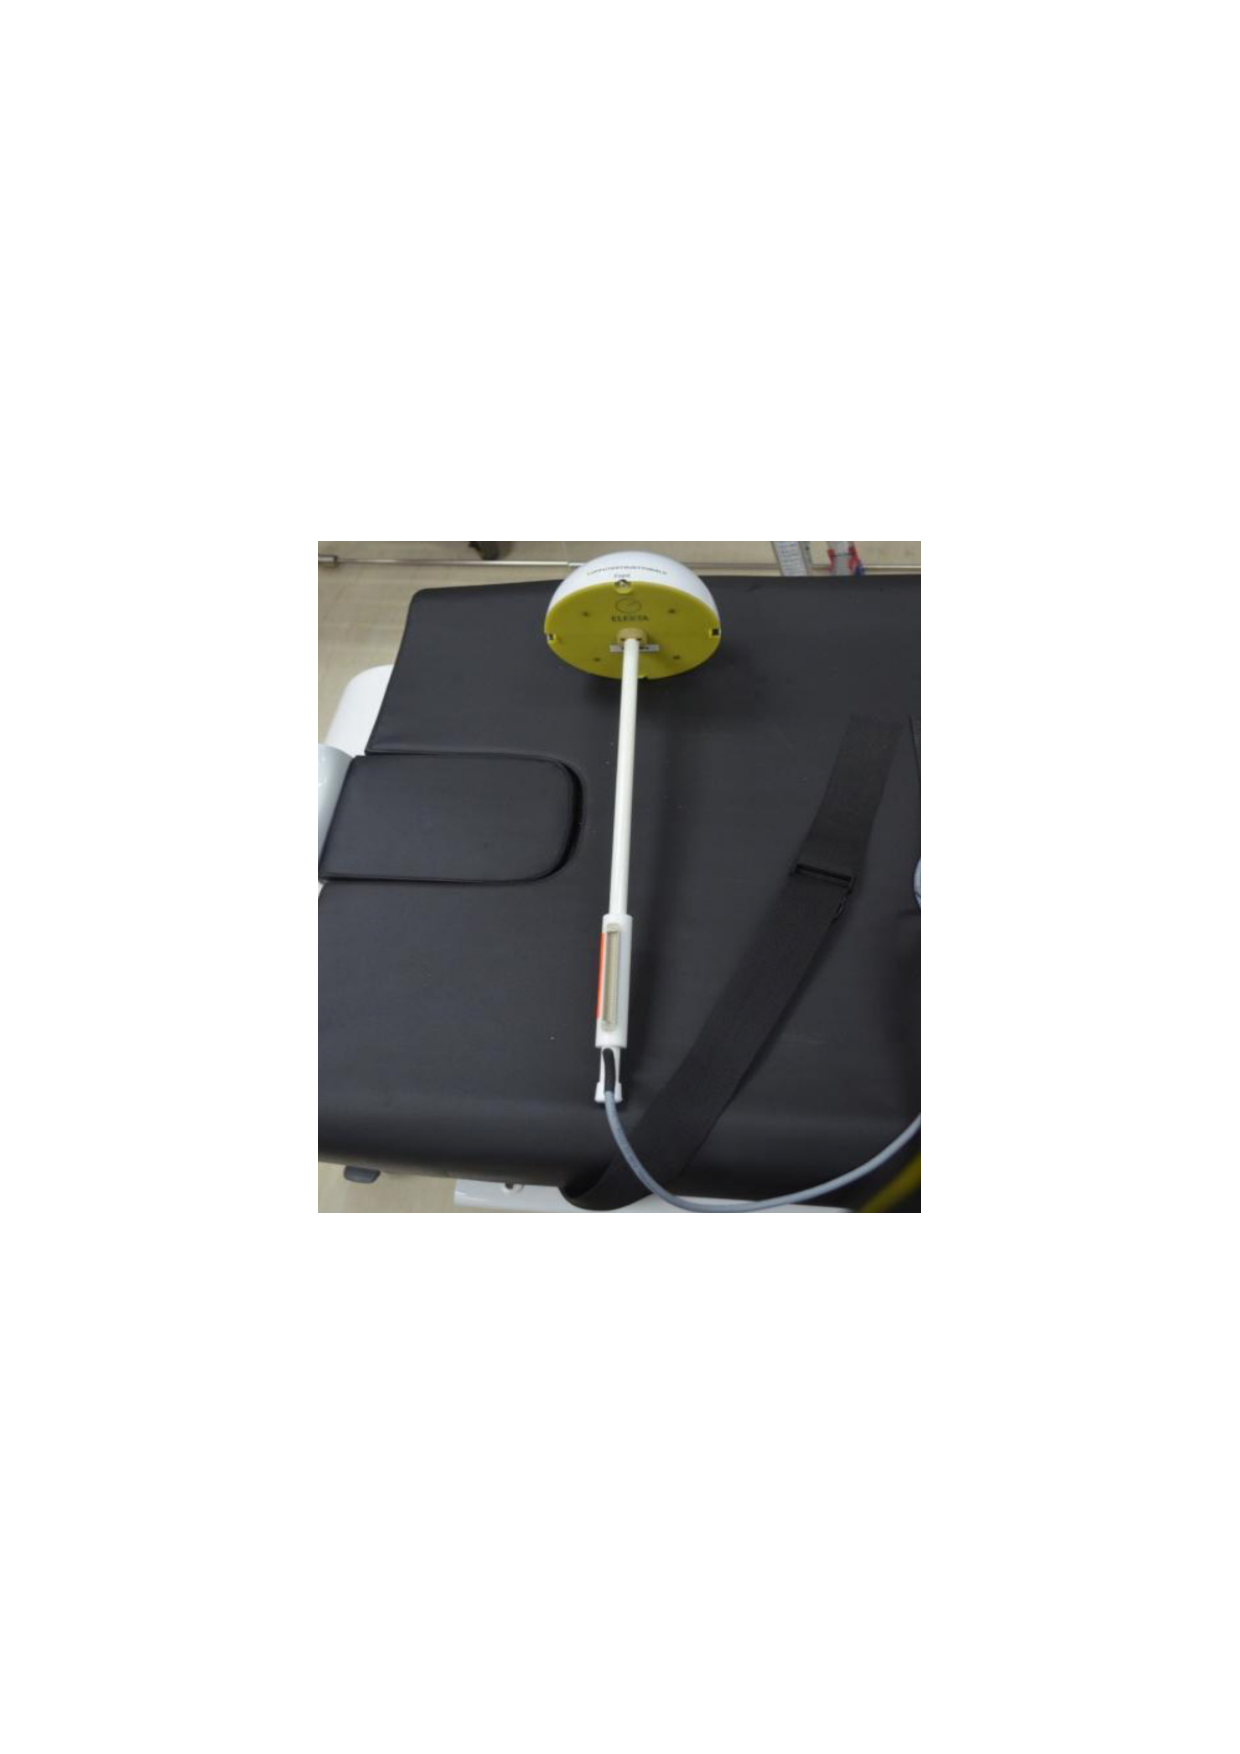
\includegraphics[trim={1cm 8cm 2cm 9cm},width = 0.97\textwidth]{benchmark/phantom_head}
\caption{Reference phantom (RefPhantom) NM24058N (Serial number: 101861) provided by Elekta Oy, Helsinki Finland. 32 built in simulated dipoles and four presetting head position indicator coils (HPI) (Figure taken from~\cite{hazim2015magnetoencephalography}).~\ref{alg:acceptreject}.}
   \label{fig:phantom_head}
\end{figure}

The phantom dipoles are energized using an internal signal generator which also feeds the HPI coils. An external multiplexer box is used to connect the signal to the individual dipoles. Only one dipole can be activated at a time. The location of the dipole is recorded relative to the center of the sphere (0,0,0), where X is positive toward the nasion, Y is positive toward the left ear and Z is positive toward the top of the head.\\

The dataset is sorted into 3 different \ac{SNR}:
\begin{itemize}
\item Source with \textbf{2000 nAm}. This corresponds to an unrealistically strong 1000 nAm (2000 nAm peak-to-peak) dipole that gives the highest SNR of the experimental source.
\item Source with \textbf{200 nAm}. This is a weaker dipole, closer to the range of amplitudes we can expect in raw data.
\item Source with \textbf{20 nAm}. This represents some of the weakest sources we expect in evoked studies which require averaging to detect and estimate (\textit{i.e.} generally cannot be seen in single trial analysis).
\end{itemize}

\subsection{Brainstorm CTF-phantom dataset}

The dataset is sorted into two different SNR:
\begin{itemize}
\item Source with \textbf{200 nAm}. This is a close dipole to the range of amplitudes we can expect in raw data.
\item Source with \textbf{20 nAm}. This represents some of the weakest sources we expect in evoked studies which require averaging to detect and estimate (\textit{i.e.} generally cannot be seen in single trial analysis).
\end{itemize}


\begin{figure}[tb]
   \centering
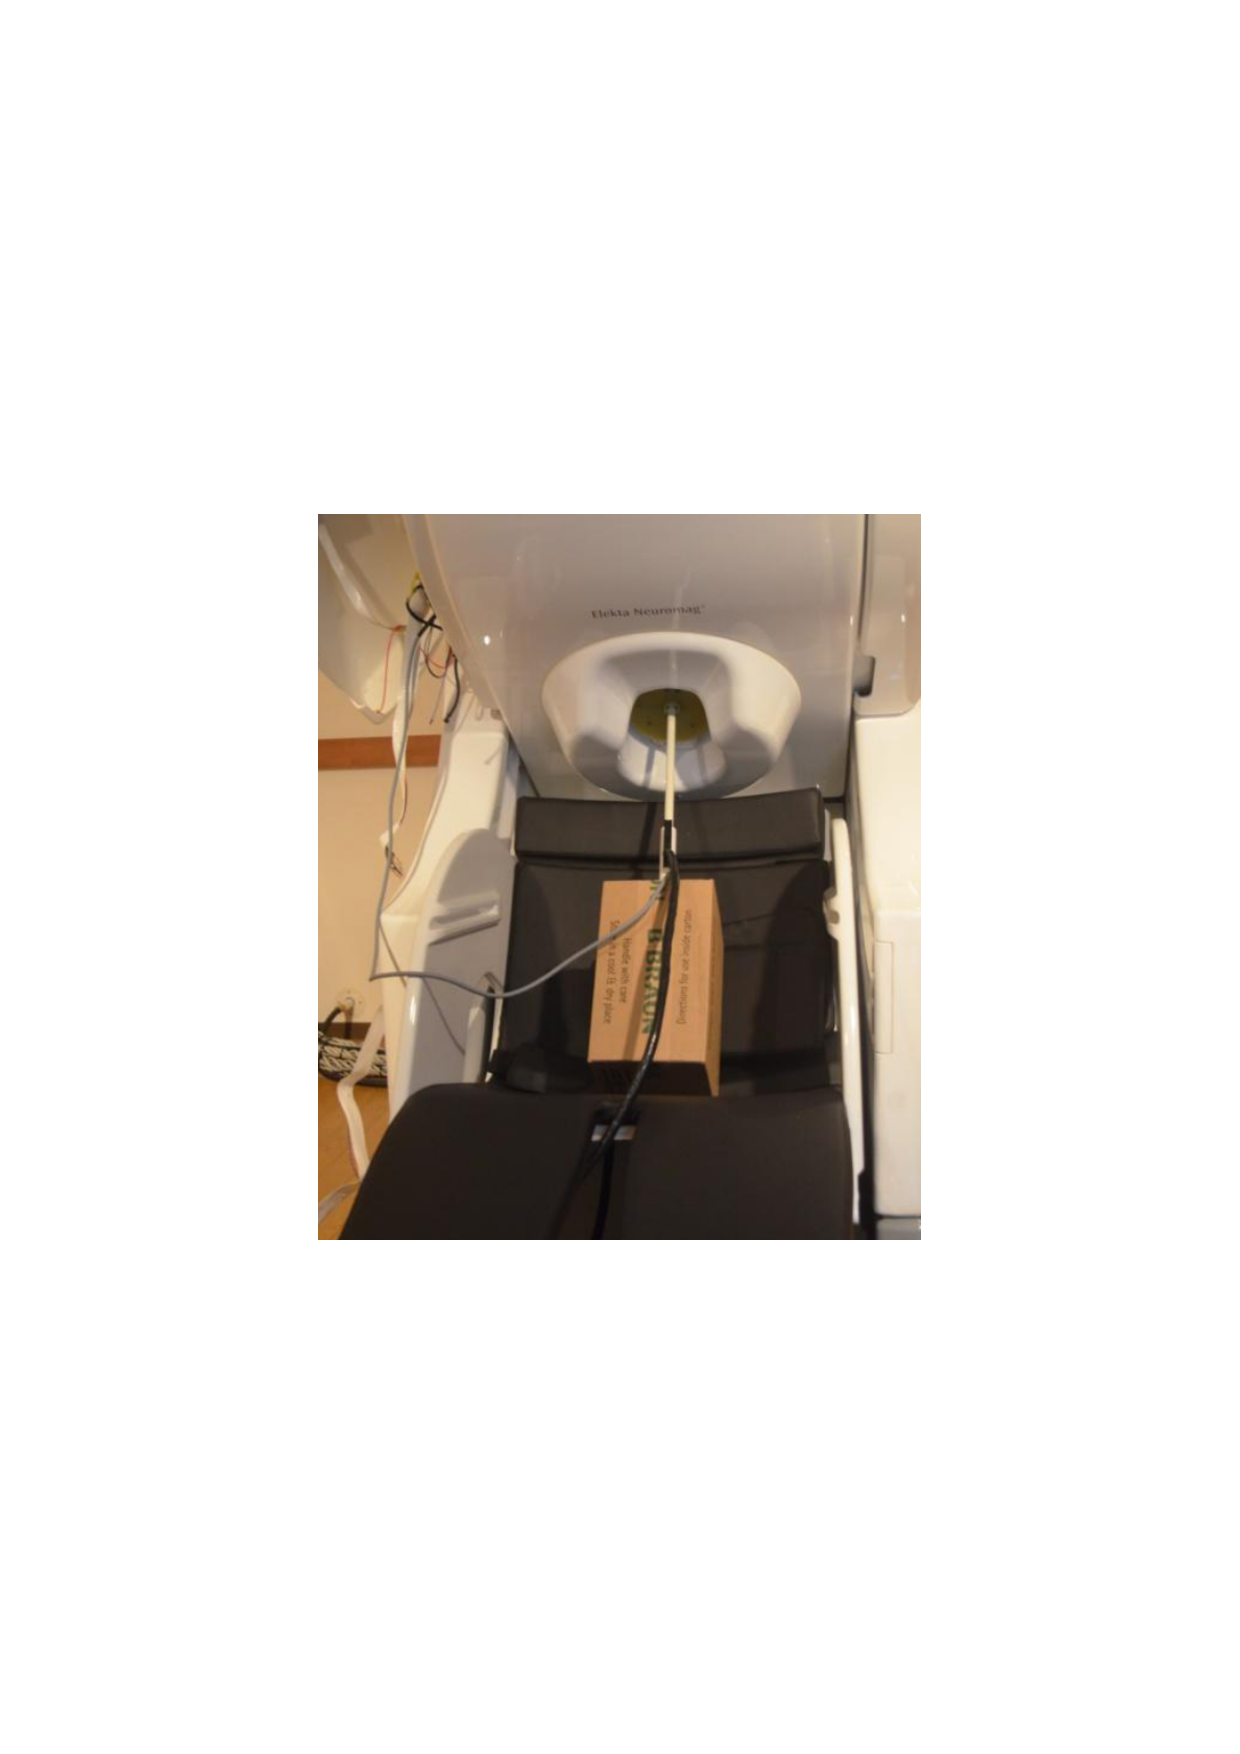
\includegraphics[trim={1cm 8cm 2cm 9cm},width = 0.97\textwidth]{benchmark/phantom_in_MEG}
\caption{Phantom is carefully set into sensor helmet of the probe unit and pushed again helmet. HPI coil is fitted into outlet under right gantry side cover (Figure taken from~\cite{hazim2015magnetoencephalography})~\ref{alg:acceptreject}.}
   \label{fig:phantom_in_MEG}
\end{figure}


\subsection{name? dataset} \label{data:used_data}

The dataset is sorted into four different SNR:
\begin{itemize}
\item Source with \textbf{2000 nAm}. This corresponds to an unrealistically strong 1000 nAm (2000 nAm peak-to-peak) dipole that gives the highest SNR of the experimental source.
\item Source with \textbf{200 nAm}. This is a weaker dipole, closer to the range of amplitudes we can expect in raw data.
\item Source with \textbf{100 nAm}. This is an even weaker dipole and a smaller SNR.
\item Source with \textbf{20 nAm}. This represents some of the weakest sources we expect in evoked studies which require averaging to detect and estimate (\textit{i.e.} generally cannot be seen in single trial analysis).
\end{itemize}

\section{Methodology}

\subsection{Sphere models}
The most commonly used head model assumes that it is made up of a set of nested concentric spheres, each with homogeneous and isotropic conductivity. Under this assumption, both the EEG and MEG problems admit to well known closed form solutions~\cite{mosher1999eeg}.

\subsection{The selected solvers}
\subsubsection{Dipole fitting}
Dipole fitting assumes that a small number of point-like \ac{ECD}s can describe the measured topography. It optimises the location, the orientation and the amplitude of the model dipoles in order to minimise the difference between the model and the measured topography. A good introduction to dipole fitting is provided by~\cite{scherg1990fundamentals}. A full description is done in Chapter~\ref{chapter:background}-Section~\ref{section_dipfit}.

\subsubsection{$\gamma$-Map}
$\gamma$-map offers a unifying view using a Bayesian perspective on some of the solvers presented here. As it was shown in Chapter~\ref{chapter:bayesian}, the Bayesian formulation of the MEG/EEG source localization consists in choosing priors/hyperpriors, estimation and inference procedure where often it boils down to alternating between the estimation of the source estimate and the estimation of the hyperparameter. The hyperparameter in this method is $\gamma$ which represents covariance components. The main idea is to use simple Gaussian mixture model with flexible covariance components, more details are in~\cite{Wipf-Nagarajan:2009}.

\subsubsection{RAP-MUSIC}
\Ac{RAP-MUSIC} is an extension to \ac{MUSIC} by recursively estimating multiple sources~\cite{mosher1997source,mosher1999source}. In other words, it consists in applying MUSIC successively after removing the contribution of the previously identified sources. Such as matching pursuit algorithms are used for sparse signal decomposition over dictionary of atoms, the RAP-MUSIC method adopts a greedy strategy to select the relevant dipoles in a dictionary of sources.

\subsubsection{MxNE | irMxNE}
\Ac{MxNE} and \ac{irMxNE} are the convex and the non-convex version of mixed-norms solvers using $\ell_{2,1}$-norm and $\ell_{2,0.5}$-quasinorm as regularizations. For more details, see Chapter~\ref{chapter:background}-Section~\ref{sec:mixed_norms} and~\cite{gramfort2012mixed,strohmeier-etal:16}.

\subsubsection{TF-MxNE | irTF-MxNE}
\Ac{TF-MxNE} and \ac{irTF-MxNE} are the convex and the non-convex version of the Time-Frequency mixed-norms using $\ell_{2,1}+\ell_1$-norm and $\ell_{2,0.5}+\ell_{0.5}$-quasinorm as regularizations. For more details, see  see Chapter~\ref{chapter:background}-Section~\ref{sec:mixed_norms} and~\cite{TF-MxNE,bekhti2016m}.

\section{Experimental results}
Three types of errors have been investigated for the different solvers, namely: the position or location error, orientation error, and amplitude error. All the solvers investigated here are implemented in the MNE-python package~\cite{mne-python,mne}.

The position error $err_{pos}$ is represented in millimeters (mm), defining the distance between the exact location ($pos_{simulated}\in\RR^3$) of the simulated dipole in the phantom head and the estimated location ($pos_{estimated}\in\RR^3$) as in Equation~\eqref{eq:pos_err}. When the estimated source space contains multiple dipoles, the one having the biggest peak of amplitude is kept and compared to the exact dipole.

\begin{equation}\label{eq:pos_err}
err_{pos} = 10^3 \|pos_{estimated} - pos{simulated}\|_{Fro}
\end{equation}

The orientation error $err_{ori}$ is represented in Radians (Rad), defining the angle between the exact orientation ($ori_{simulated}\in\RR^3$) of the simulated dipole and the estimated one ($ori_{estimated}\in\RR^3$) as in Equation~\eqref{eq:ori_err}. Same for the position error, the best dipole is kept when multiple ones are estimated.

\begin{equation}\label{eq:ori_err}
err_{ori} = arccos(|<ori_{estimated}, ori_{simulated}>|)
\end{equation}

Finally, the amplitude error $err_{amp}$is represented in nanoAmpere (nAm) except for some solvers which give source estimates with statistical values and not electrical current values (example: dSPM). This error defines the difference between the peak of amplitude ($max(amp_{estimated}) with amp_{estimated}\in\RR^T$) of the estimated dipole and the peak of simulated dipole $amp_{simulated}\in\RR$ (example 1000nAm, 200nAm, ... 20nAm) as in Equation~\eqref{eq:amp_err}.

\begin{equation}\label{eq:amp_err}
err_{amp} = |max(amp_{estimated} - amp_{simulated})|
\end{equation}

Figures showing the three types of error over different solvers are displayed below. On the x-axis, three different pre-processing types are presented:
\begin{itemize}
\item \textit{Raw}: the source localization is using the raw data without applying maxfilter.
\item \textit{SSS}: the source localization is applying Signal Space Separation (SSS), also known as maxfilter. It is the first step of preprocessing MEG data, which is a clever mathematical way to separate magnetic signals coming from the brain from those coming from outside the brain.
\item \textit{$SSS_{MNE}$}: the source localization is applying a new implementation of maxfilter in MNE-python.
\end{itemize}

Figure~\ref{fig:dipfit_errors} shows position errors obtained with dipole fitting method for the 4 simulated dipoles (dataset \ref{data:used_data}) and for the different SNRs. Figure~\ref{fig:dipfit_pos} shows less than 1mm error for the unrealistic high SNR (peak-to-peak amplitude equal to 1000nAm), but also for 200nAM, and 100nAm. The location error gets worse with the very low SNR (20nAm).
%\subsection*{dipfit}

\begin{sidewaysfigure}[ht]
        \centering
        \begin{subfigure}[b]{0.28\textwidth}
            \centering
            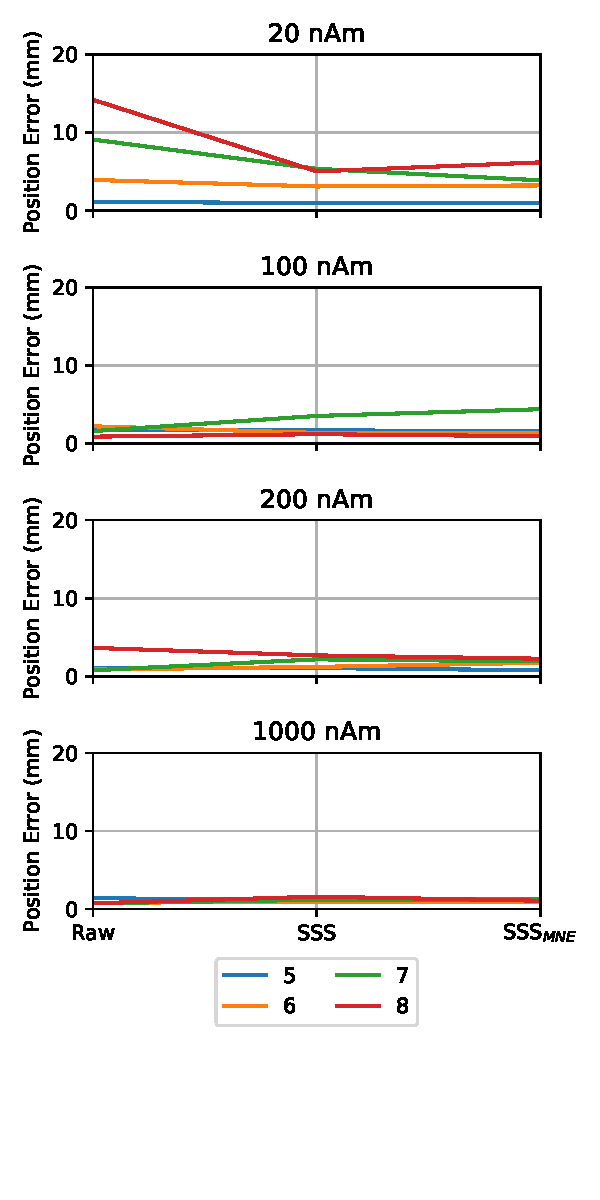
\includegraphics[trim={1cm 2.5cm 1cm 1cm},width=\textwidth]{benchmark/phantom_errors_dipfit_loc_error}
            \caption{\label{fig:dipfit_pos}}
        \end{subfigure}
		\hspace{35pt}
        \begin{subfigure}[b]{0.28\textwidth}  
            \centering 
            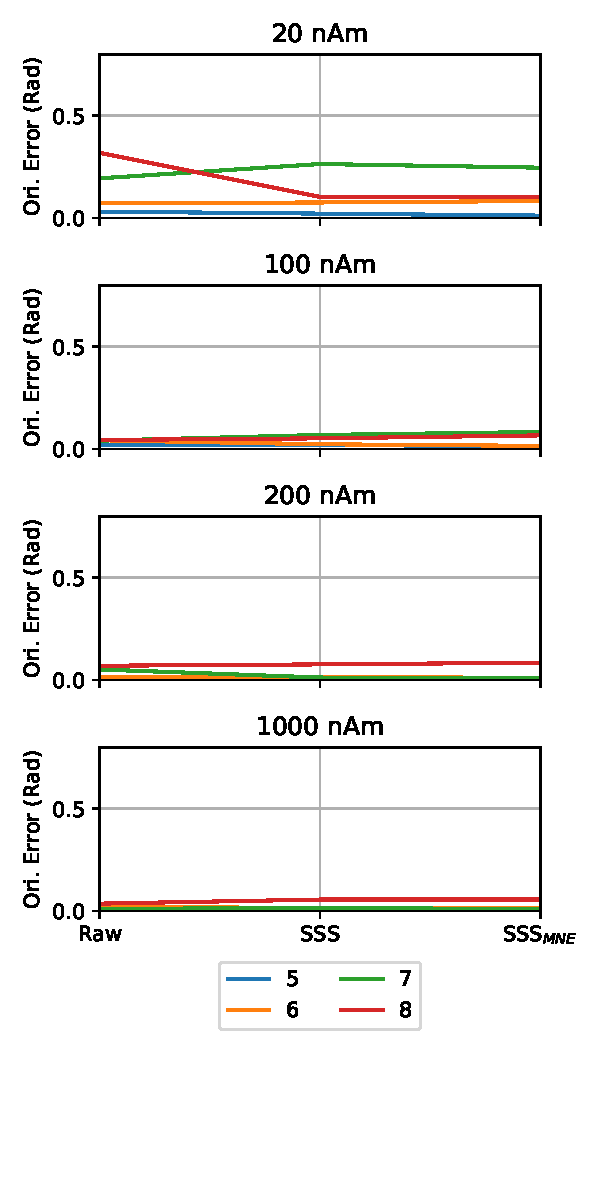
\includegraphics[trim={1cm 2.5cm 1cm 1cm},width=\textwidth]{benchmark/phantom_errors_dipfit_ori_error}
            \caption{\label{fig:dipfit_ori}}
        \end{subfigure}
		\hspace{35pt}
        \begin{subfigure}[b]{0.28\textwidth}   
            \centering 
            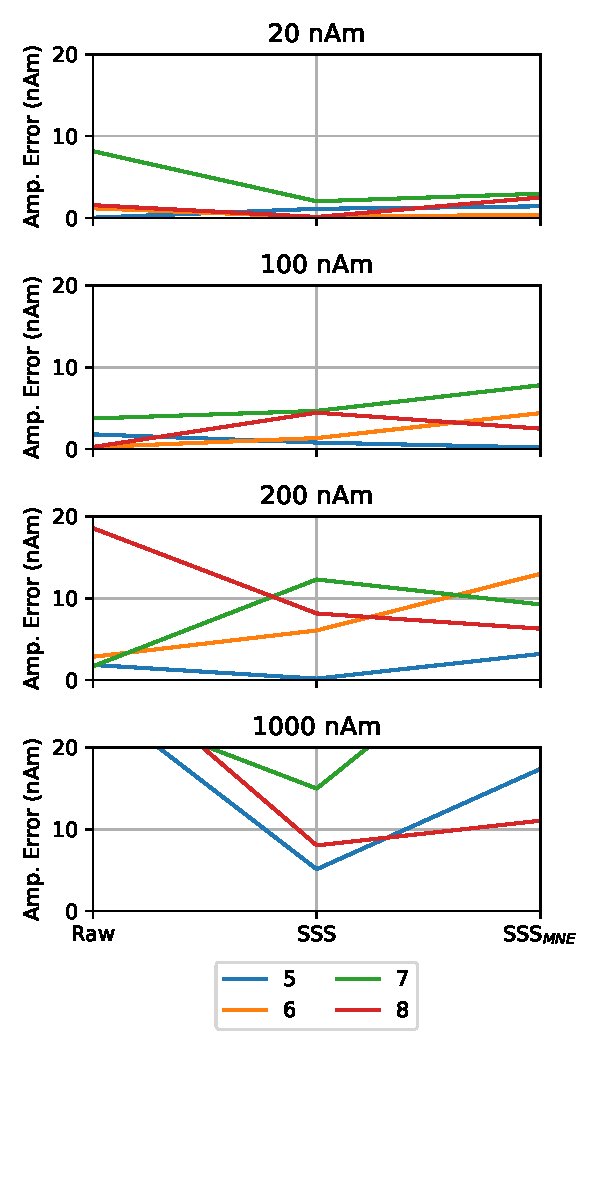
\includegraphics[trim={1cm 2.5cm 1cm 1cm},width=\textwidth]{benchmark/phantom_errors_dipfit_amp_error}
            \caption{\label{fig:dipfit_amp}}
        \end{subfigure}

		\caption{The dipole fit errors on localization (mm), orientation (Rad), and amplitude (nAm) using 4 dipoles (5-8) having different depth in the phantom.\label{fig:dipfit_errors}}
\end{sidewaysfigure}

Dipole fitting approach is very suitable to localize the neuronal activity when a small number of \ac{ECD}s can describe the data. In this dataset \ref{data:used_data}, each dipole is recorded alone. The errors in orientations and amplitude are in Figure \ref{fig:dipfit_ori}-\ref{fig:dipfit_amp}.

RAP-MUSIC is an approach based on MUSIC technique which also perform very well when few ECDs are involved, especially when it is a dataset recording only one dipole in a row. It can be seen as very competitive to dipole fitting in Figure \ref{fig:music_pos}-\ref{fig:music_ori}-\ref{fig:music_amp} showing the errors in position, orientation, and amplitude respectively. However, for deep source (dipole 8) combined with very low SNR (20nAm) the red curve is outside of the box meaning a location error bigger than 20mm. This is an issue with the signal subspace estimation, where the rank of the data covariance is not being well estimated.

%\subsection*{MUSIC}
\begin{sidewaysfigure}[ht]
        \centering
        \begin{subfigure}[b]{0.28\textwidth}
            \centering
            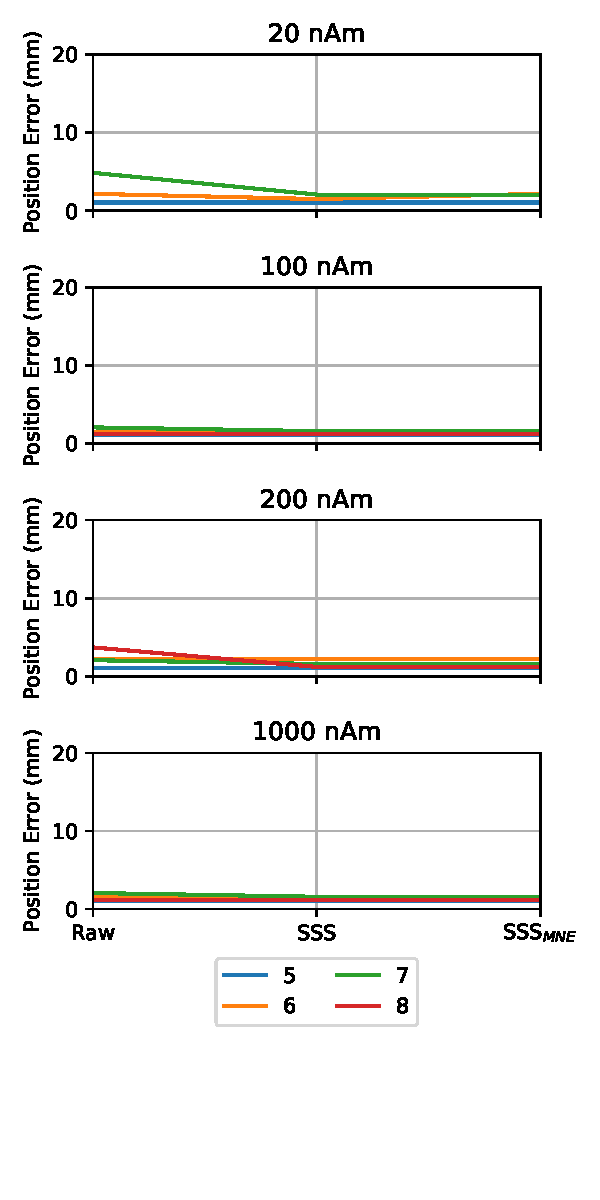
\includegraphics[trim={1cm 2.5cm 1cm 1cm},width=\textwidth]{benchmark/phantom_errors_music_loc_error}
            \caption{\label{fig:music_pos}}
        \end{subfigure}
		\hspace{35pt}
        \begin{subfigure}[b]{0.28\textwidth}  
            \centering 
            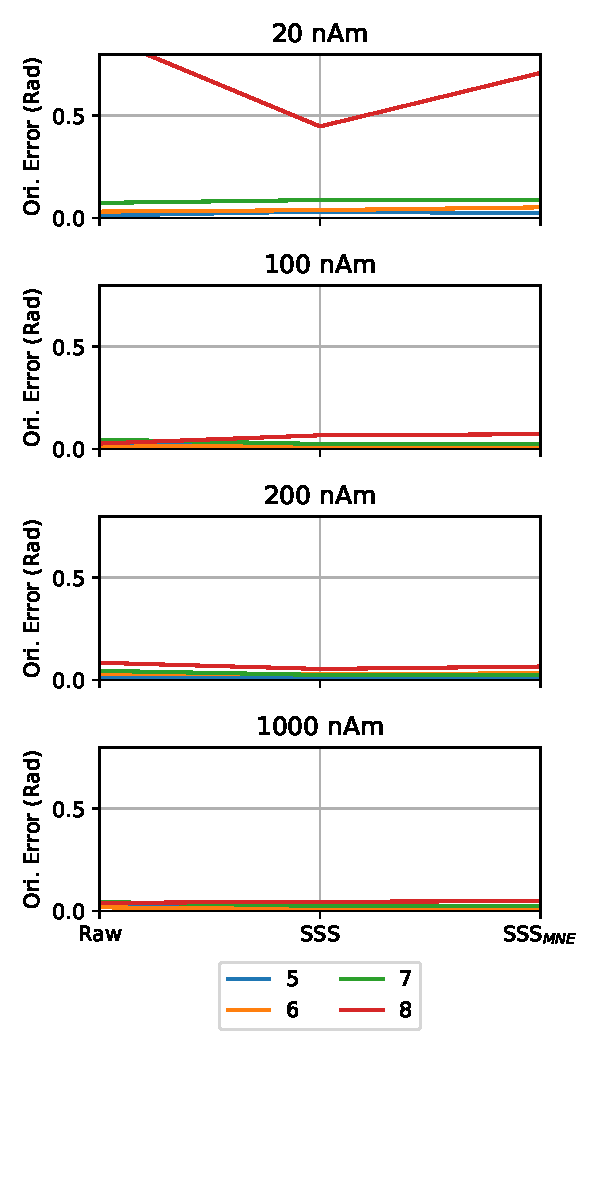
\includegraphics[trim={1cm 2.5cm 1cm 1cm},width=\textwidth]{benchmark/phantom_errors_music_ori_error}
            \caption{\label{fig:music_ori}}
        \end{subfigure}
		\hspace{35pt}
        \begin{subfigure}[b]{0.28\textwidth}   
            \centering 
            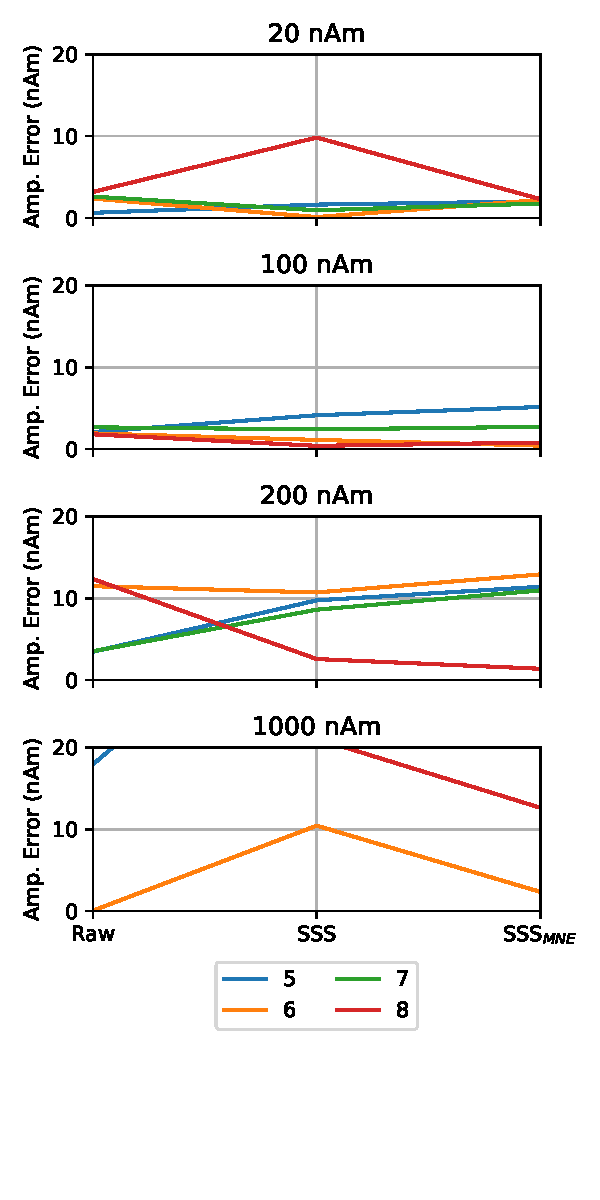
\includegraphics[trim={1cm 2.5cm 1cm 1cm},width=\textwidth]{benchmark/phantom_errors_music_amp_error}
            \caption{\label{fig:music_amp}}
        \end{subfigure}

		\caption{The MUSIC errors on localization (mm), orientation (Rad), and amplitude (nAm) using 4 dipoles (5-8) having different depth in the phantom.\label{fig:music_errors}}
\end{sidewaysfigure}


%\subsection*{Gamma map}
\begin{sidewaysfigure}[ht]
        \centering
%        \vspace{10pt}
        \begin{subfigure}[b]{0.28\textwidth}
            \centering
            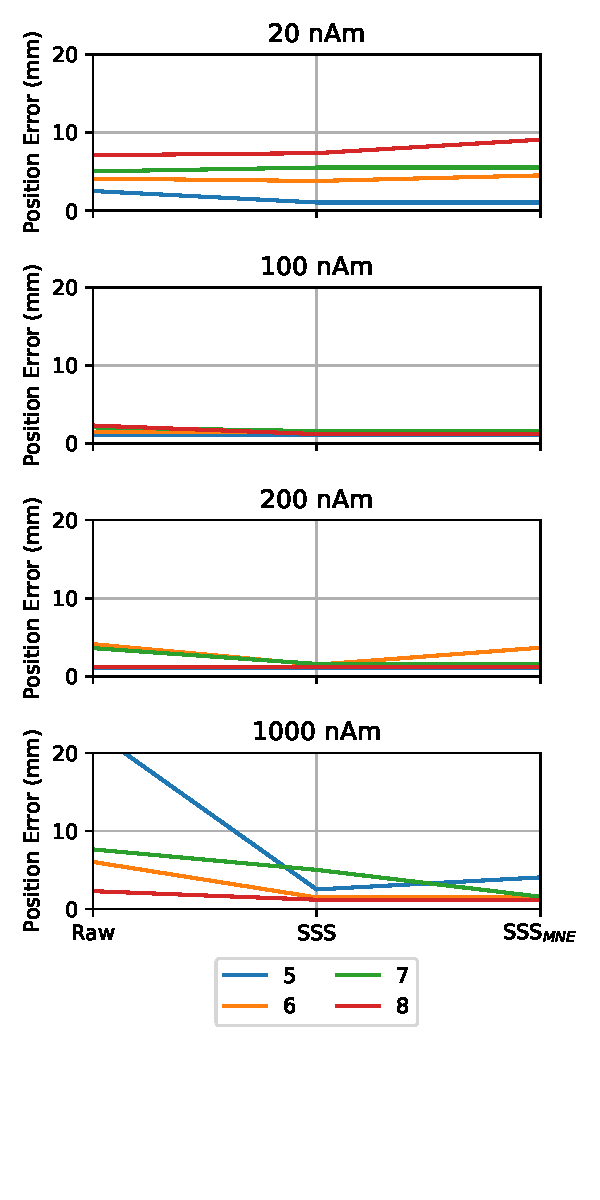
\includegraphics[trim={1cm 2.5cm 1cm 1cm},width=\textwidth]{benchmark/phantom_errors_gamma_map_loc_error}
%            \caption{pos}
            \label{fig:gmap_pos}
        \end{subfigure}
%        \hfill
		\hspace{35pt}
        \begin{subfigure}[b]{0.28\textwidth}  
            \centering 
            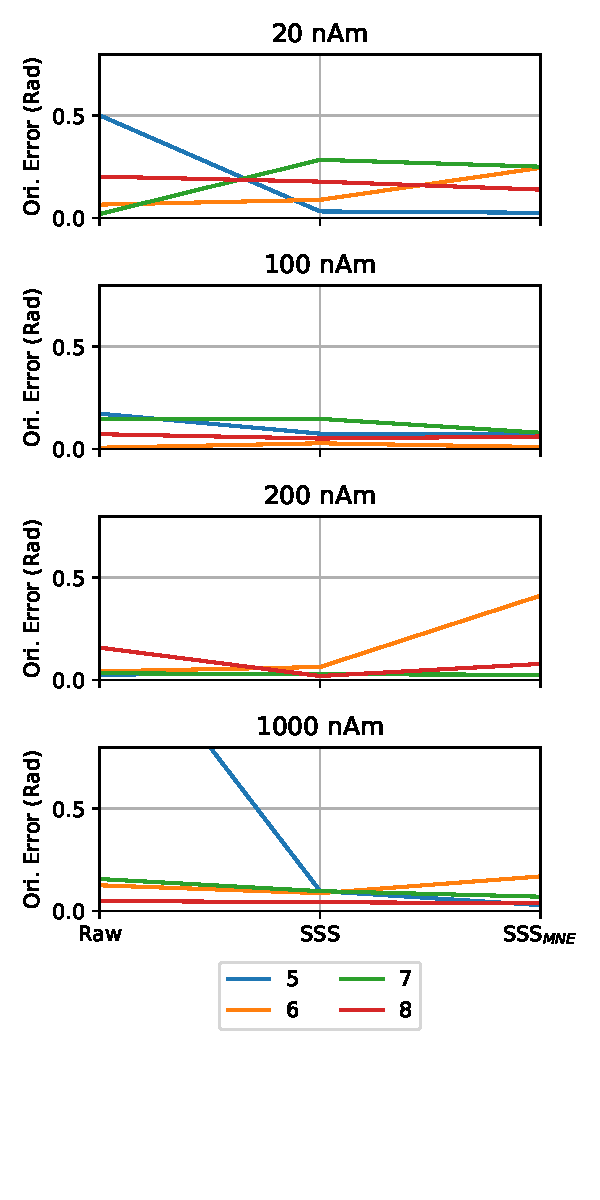
\includegraphics[trim={1cm 2.5cm 1cm 1cm},width=\textwidth]{benchmark/phantom_errors_gamma_map_ori_error}
%            \caption{ori}
            \label{fig:gmap_ori}
        \end{subfigure}
%        \vskip\baselineskip
		\hspace{35pt}
        \begin{subfigure}[b]{0.28\textwidth}   
            \centering 
            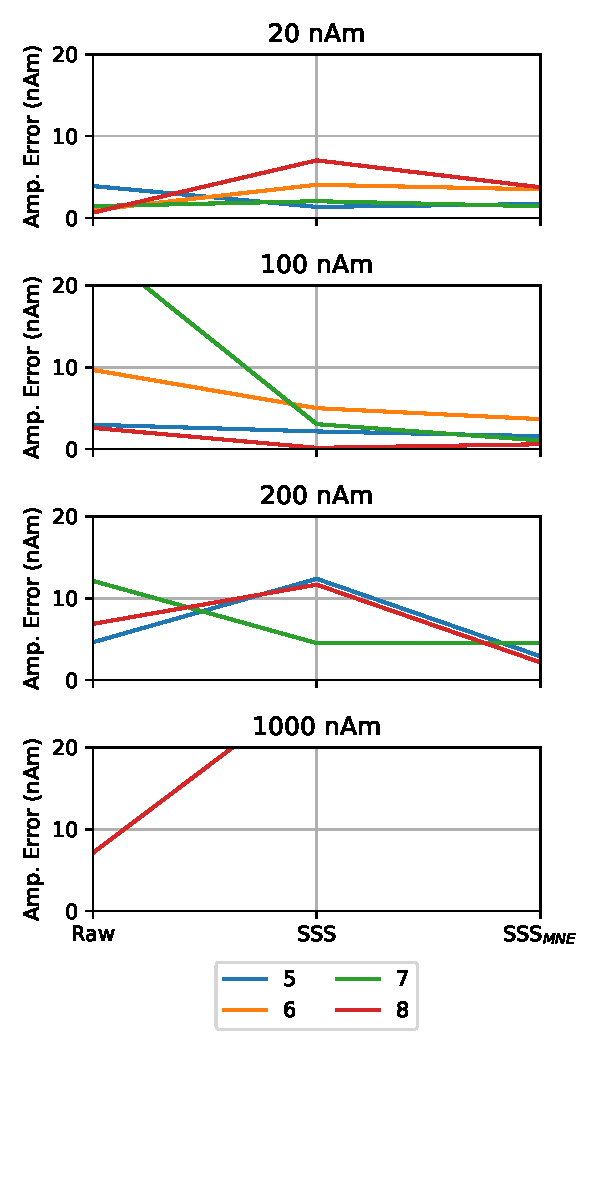
\includegraphics[trim={1cm 2.5cm 1cm 1cm},width=\textwidth]{benchmark/phantom_errors_gamma_map_amp_error}
%            \caption{amp}
            \label{fig:gmap_amp}
        \end{subfigure}

		\caption{The gamma map errors on localization (mm), orientation (Rad), and amplitude (nAm) using 4 dipoles (5-8) having different depth in the phantom.\label{fig:gmap_errors}}
\end{sidewaysfigure}


%\subsection*{Mixed norm (MxNE)}
\begin{sidewaysfigure}[ht]
        \centering
%        \vspace{10pt}
        \begin{subfigure}[b]{0.28\textwidth}
            \centering
            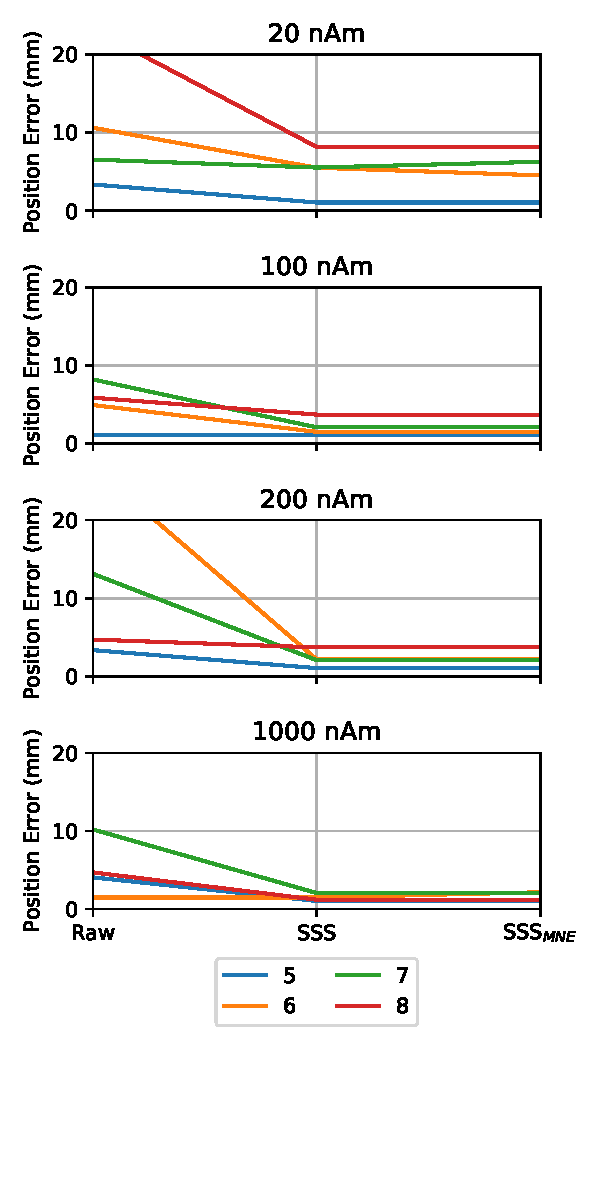
\includegraphics[trim={1cm 2.5cm 1cm 1cm},width=\textwidth]{benchmark/phantom_errors_MxNE_loc_error}
%            \caption{pos}
            \label{fig:mxne_pos}
        \end{subfigure}
%        \hfill
		\hspace{35pt}
        \begin{subfigure}[b]{0.28\textwidth}  
            \centering 
            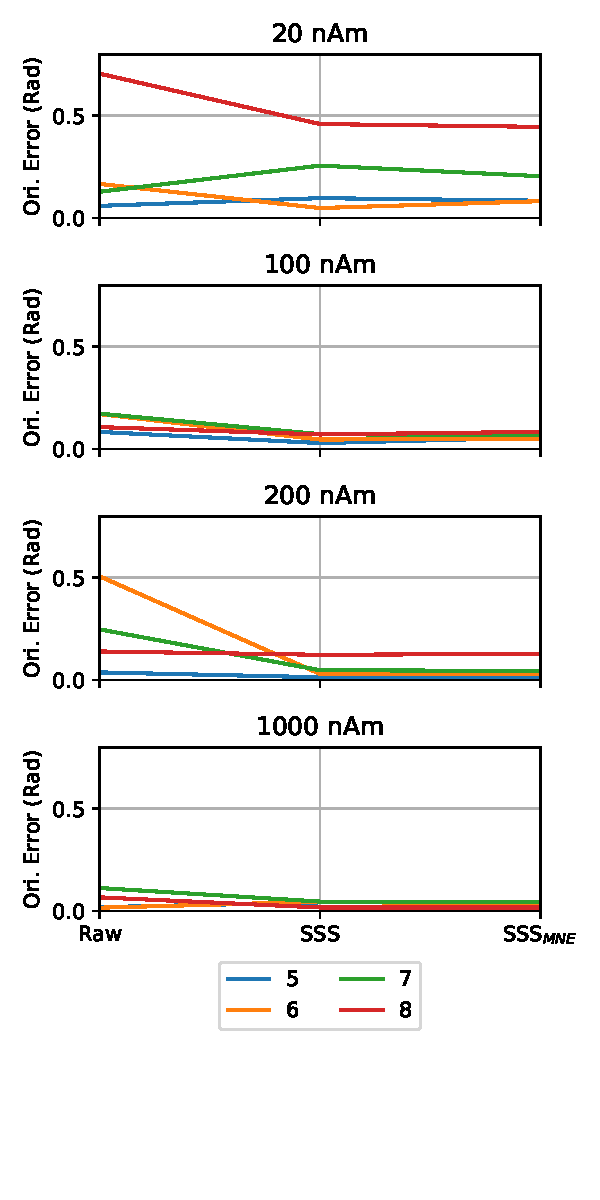
\includegraphics[trim={1cm 2.5cm 1cm 1cm},width=\textwidth]{benchmark/phantom_errors_MxNE_ori_error}
%            \caption{ori}
            \label{fig:mxne_ori}
        \end{subfigure}
%        \vskip\baselineskip
		\hspace{35pt}
        \begin{subfigure}[b]{0.28\textwidth}   
            \centering 
            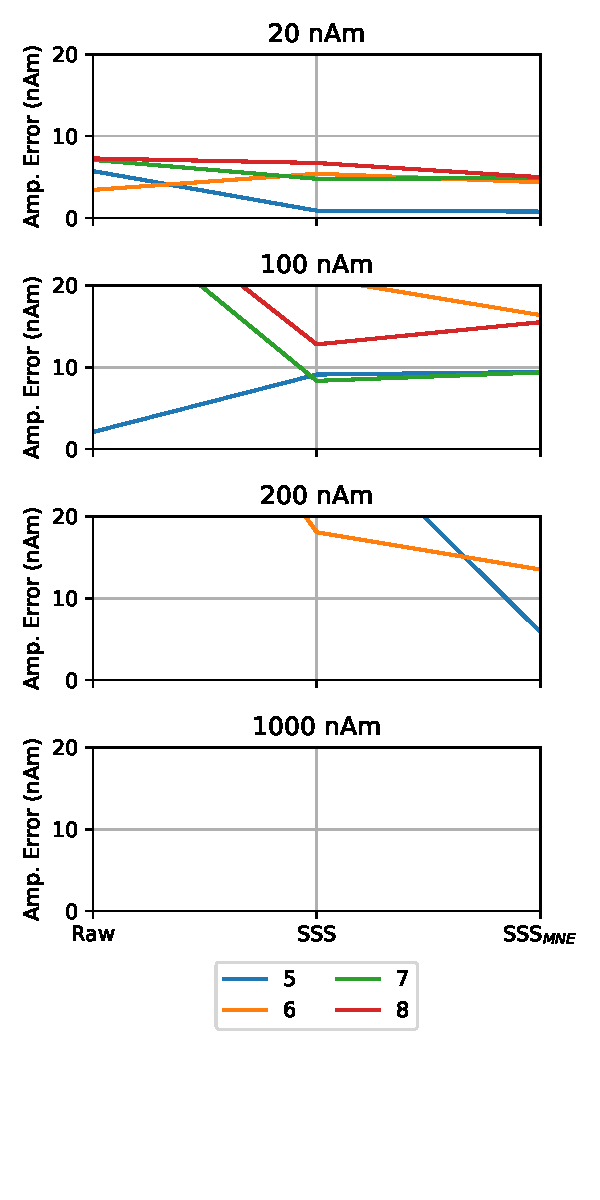
\includegraphics[trim={1cm 2.5cm 1cm 1cm},width=\textwidth]{benchmark/phantom_errors_MxNE_amp_error}
%            \caption{amp}
            \label{fig:mxne_amp}
        \end{subfigure}

		\caption{The mixed norm (MxNE) errors on localization (mm), orientation (Rad), and amplitude (nAm) using 4 dipoles (5-8) having different depth in the phantom.\label{fig:gmap_errors}}
\end{sidewaysfigure}

%\subsection*{Time-Frequency mixed-norm (TF-MxNE)}
\begin{sidewaysfigure}[ht]
        \centering
%        \vspace{10pt}
        \begin{subfigure}[b]{0.28\textwidth}
            \centering
            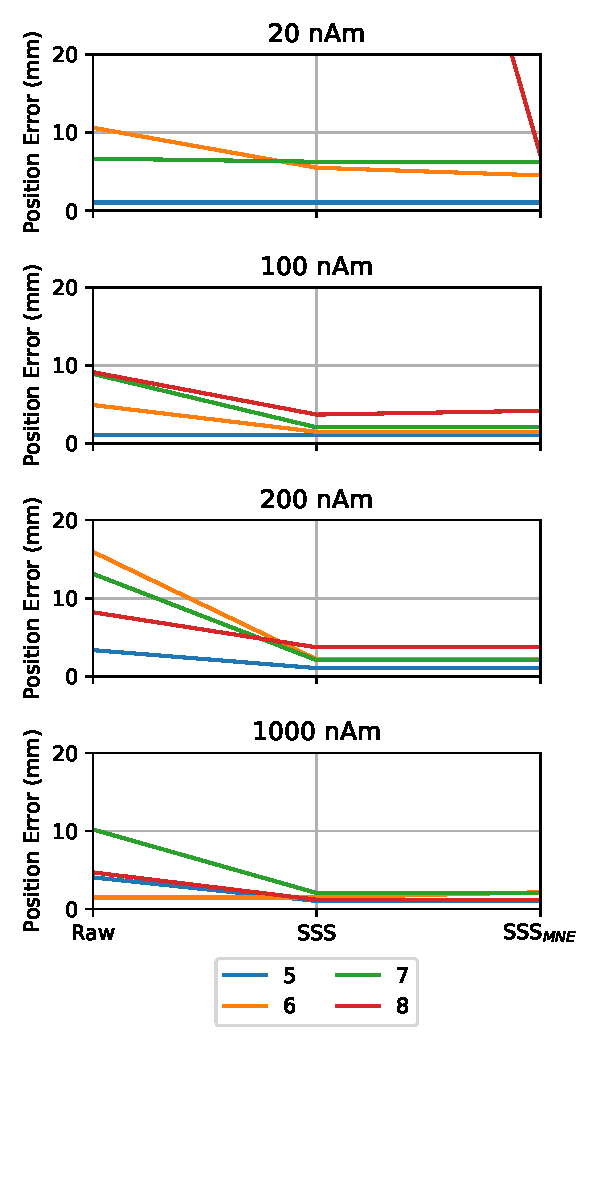
\includegraphics[trim={1cm 2.5cm 1cm 1cm},width=\textwidth]{benchmark/phantom_errors_TF-MxNE_loc_error}
%            \caption{pos}
            \label{fig:tfmxne_pos}
        \end{subfigure}
%        \hfill
		\hspace{35pt}
        \begin{subfigure}[b]{0.28\textwidth}  
            \centering 
            \includegraphics[trim={1cm 2.5cm 1cm 1cm},width=\textwidth]{benchmark/phantom_errors_TF-MxNE_ori_error}
%            \caption{ori}
            \label{fig:tfmxne_ori}
        \end{subfigure}
%        \vskip\baselineskip
		\hspace{35pt}
        \begin{subfigure}[b]{0.28\textwidth}   
            \centering 
            \includegraphics[trim={1cm 2.5cm 1cm 1cm},width=\textwidth]{benchmark/phantom_errors_TF-MxNE_amp_error}
%            \caption{amp}
            \label{fig:tfmxne_amp}
        \end{subfigure}

		\caption{The time-frequency mixed-norm (TF-MxNE) errors on localization (mm), orientation (Rad), and amplitude (nAm) using 4 dipoles (5-8) having different depth in the phantom.\label{fig:tfmxne_errors}}
\end{sidewaysfigure}

$\gamma$-map which is a Bayesian formulation to the MEG/EEG inverse problem is performing less well than dipole fitting or RAP-MUSIC for very high and very low SNR. For SNRs in range of realistic data, its location error is majored by 5mm depending on the depth of the studied dipole. $\gamma$-map is doing worse for amplitude=1000nAm compared to 100nAm or 200nAm because it overestimates the noise when estimating the hyperparameter $\gamma$.

For MxNE and TF-MxNE, the errors shown in Figure~\ref{fig:mxne_pos}-\ref{fig:tfmxne_pos} respectively demonstrate an improvement more the SNR is high.

\subsection{Critical comparison of these MEG/EEG source localization}
Figure \ref{all_solvers_loc_error} shows all solvers in the same plot to compare both errors in location and orientation with maxfilter as preprocessing. We keep the same scale for y-axis to not go beyond 20 mm of location error and not beyond 1 Rad of orientation error. The left plot of location error shows firstly (RAP) MUSIC as being very sensitive the SNR (comparing 20nAm to 1000nAm). Then MNE and dSPM as the methods giving the worst results for this dataset. One important argument is the fact that the study is biased as we know that the simulated phantom data is focal/sparse, while MNE and dSPM are not sparse methods. We always take the peak of amplitude and displays the best dipole for each method. sLORETA in the other hand is not a sparse method either, however, it performs much better than MNE or dSPM. The "center" of the pattern estimated with sLORETA is then closer to the exact dipole location compared to the center of dSPM or MNE. TF-MxNE is not the best method for this study as it is a spatio-temporal approach when having a specific waveforms in the data which is not the case here.

\begin{sidewaysfigure}[ht]
        \centering
%        \vspace{10pt}
        \begin{subfigure}[b]{0.47\textwidth}
            \centering
            \includegraphics[trim={1cm 2.5cm 1cm 1cm},width=\textwidth]{benchmark/phantom_errors_all_solvers_maxfilter_True_loc_error}
%            \caption{pos}
            \label{fig:all_solvers_loc_error}
        \end{subfigure}
%        \hfill
		\hspace{25pt}
        \begin{subfigure}[b]{0.47\textwidth}  
            \centering 
            \includegraphics[trim={1cm 2.5cm 1cm 1cm},width=\textwidth]{benchmark/phantom_errors_all_solvers_maxfilter_True_ori_error}
%            \caption{ori}
            \label{fig:all_solvers_ori_error}
        \end{subfigure}

		\caption{Comparison of the position and the orientation error between most of the solvers for 4 different dipoles.\label{all_solvers_loc_error}}
\end{sidewaysfigure}

The orientation error is comparable to the location error, where dipole fitting, MUSIC, $\gamma$-map, MxNE and irMxNE keeps being the best performing methods. Dipole fitting is unbeatable when simulating with only one dipole. We could not sum up dipoles to make the simulation even harder, because their locations is nearly the same except the depth is different. When summing up this type of dipole, they still have the same pattern in the sensor space, which makes the source localization impossible.

\begin{figure}
	\includegraphics[width=\textwidth]{benchmark/phantom_errors_all_solvers_maxfilter_True_amp_error}
	\caption{Comparison of amplitude error between most of the solvers for 4 different dipoles.\label{all_solvers_amp_error}}
\end{figure}

Figure~\ref{all_solvers_amp_error} shows the errors in amplitude, the most important point in this figure is to see the difference between the convex MxNE and the non-convex irMxNE in terms of amplitude bias. All dipoles basically improve their amplitude estimate when using the non-convex method (irMxNE). For some cases, irMxNE amplitude estimate is even better than dipole fitting one.


\section{Conclusion \& Perspectives}
In this chapter, the main motivation was to present some results on various source localization techniques applied to phantom data. Being able to examine "real" datasets with ground-truth is a big privilege to test the big list of existing methods for solving the MEG/EEG inverse problem.

Here we presented some of them, focusing on the approaches defined in this thesis. The conclusion would be that the dipole fitting is the most competitive and unbeatable method when having a focal dataset with only one dipole. Unfortunately here, we could not present phantom dataset with two or more dipoles in the same recording, which would make the source localization more challenging.

A further work would be to investigate this aspect of multiple dipoles. The idea would be to confirm a better performance of convex and non-convex solvers (Variational or Bayesian formulation) compared to dipole fitting or MUSIC.
% Chapter 5

\chapter{Decoding visual motion from MEG}
\label{chapter:decoding}
\section{Introduction - Context}
\section{Experimental design \& Participants}
\section{MEG pre-processing \& source localization}
\section{MEG decoding}
\section{Results \& Discussion}
\section{Conclusion}

\frontmatter
% Chapter 5

\chapter{Conclusion \& Perspectives}
\label{chapter:conclusion}

This thesis demonstrated various ways to solve the MEG/EEG source localization problem. It tackles specific challenges faced by current state-of-the-art techniques, and tries to improve them point by point:
\begin{itemize}
\item Promoting structured sparsity in the TF domain has been proved to suitable for reconstructing non-stationary sources, although it needs to fix some parameters related to the Gabor transform, which are involved in the TF resolution. The first improvement proposed in this thesis was to tackle the choice of these parameters, which can be very detrimental for the analysis of brain waves with variable TF characteristics. It provides a new technique based on a multi-scale TF mixed norm allowing us to more accurately localize the source estimated in space and time (see Chapter~\ref{chapter:multiscale}).

\item The formulation of the MEG/EEG inverse problem has been mostly written as a penalized regression, meaning that it needs to introduce a prior knowledge as a regularization term into the objective function. This results in adding a hyperparameter to the model which needs to be tuned. This thesis tackles this second challenge in two ways, both reformulating the problem as done in the Bayesian community. The Bayesian formulation allows to hierarchically add hyperparameters that are alternatively estimated with the main parameters of the model (the sources). The two main advantages are: the direct estimation of the hyperparameters, and the ability to use sampling in order to investigate the uncertainty of these solvers. These two points were presented in Chapter~\ref{chapter:bayesian}.

\item An important step after developing any new technique is to validate it with a comparison with the other existing methods. This has for a long been a hard step as it is always hard to develop good and realistic simulations, where to apply the new techniques. For this aim, several studies have been investigating phantom dataset, which is a dataset of a mimic phantom head replicating a realistic environment. Chapter~\ref{chapter:benchmark} shows a comparison of the solvers presented in this thesis on phantom datasets.
\end{itemize}

This thesis was based on a long research line started by my supervisor Alexandre Gramfort, and then his former PhD Student Daniel Strohmeier, and was meant to improve several parts of the MEG/EEG source localization issues encountered so far. The points cited before were mainly the ones developed in this thesis, however several non-trivial ones remain open questions for further work to make best use of the available neuroimaging data:
\begin{itemize}
\item Although we found a way to solve the problem of source localization in the TF domain when having a mixture of brain signals in the data, it is still a non-trivial task to set the parameters of the multi-scale dictionary. As presented before, another possible way is to learn models that are good enough to capture the rich frequency content, and the morphology of the brain signal. The dictionary learning research line has given pretty nice results so far on electrophisiological signals~\cite{jas2017learning,jost2006motif,brockmeier2016learning,hitziger2017adaptive}, which makes the technique completely autonomous and data-driven.

\item The spatio-temporal techniques presented in this thesis are designed for the analysis of averaged evoked responses to ensure a descent SNR. Future work can be directed on how to make these techniques applicable on single trial data. A possible idea is to localize each trial separately by imposing an additional constraint onto the model, such as the active set must be consistent over all trials~\cite{strohmeier2012meg,strohmeier2012biomag}.

\item While invoking new constraints onto the model, another line of future work can be on the optimization side for solving the MEG/EEG inverse problem. In machine learning, various papers have been investigating mathematical and computational challenges to better tackle the inverse problem in general. One possible direction for the MEG/EEG inverse problem is to improve the computational complexity, because the proposed approaches need to be competitive in terms of running time. This results in research lines such as how to fasten the algorithms; a practical example which was used in this thesis is the use of an active set. A more sophisticated approach would be to apply screening rules, \textit{i.e.} find in advance the involved sources in order to compute the solution only for them, and avoid spending time on computing sources which will be inactive at the end~\cite{fercoq-etal:2015,massias2017safe,massiasgap,ndiaye2016gap,ndiaye2017efficient}.

\item The proposed method in the TF domain still lacks an automatic model selection criterion to set the two regularization hyperparameters (one over space, the second over time). Chapter~\ref{chapter:bayesian} presented a way to automatically set the hyperparameter for the mixed norm (MxNE) approach, which has only one regularization parameter over space. A further work can rewrite the problem for TF-MxNE, or investigate other model selection criteria.

\item The novel methods and some of state-of-the-art approaches have been tested using three phantom datasets. A future work would be to investigate more in depth this validation to compare their capabilities with a more sophisticated data, \textit{i.e.}, two or more dipoles in a row, instead of only one dipole as presented here.
\end{itemize} 


%----------------------------------------------------------------------------------------
%	THESIS CONTENT - APPENDICES
%----------------------------------------------------------------------------------------

%\appendix % Cue to tell LaTeX that the following "chapters" are Appendices

% Include the appendices of the thesis as separate files from the Appendices folder
% Uncomment the lines as you write the Appendices

%% Appendix A

\chapter{Appendix Title Here} % Main appendix title

\label{AppendixA} % For referencing this appendix elsewhere, use \ref{AppendixA}

Write your Appendix content here.
%\include{Appendices/AppendixB}
%\include{Appendices/AppendixC}

%----------------------------------------------------------------------------------------
%	BIBLIOGRAPHY
%----------------------------------------------------------------------------------------

\clearpage

\printbibliography[heading=bibintoc]

%----------------------------------------------------------------------------------------

\end{document}  
